% !TeX program = xelatex
\documentclass[11pt,a4paper,oneside]{article}
\usepackage[margin=25mm,headheight=15pt]{geometry}
\usepackage[T1]{fontenc}
\usepackage{lmodern}
\usepackage{amsmath,amssymb,amsthm,mathtools,bm,mathrsfs}
\usepackage{booktabs,longtable,array,graphicx,calc}
\usepackage{textcomp,etoolbox}
\AtBeginEnvironment{longtable}{\small}
\allowdisplaybreaks[2]
\AtBeginDocument{%
  \apptocmd{\normalsize}{%
  \setlength{\abovedisplayskip}{7pt plus 2pt minus 3pt}%
  \setlength{\belowdisplayskip}{7pt plus 2pt minus 3pt}%
  \setlength{\abovedisplayshortskip}{0pt plus 2pt}%
  \setlength{\belowdisplayshortskip}{5pt plus 2pt minus 2pt}%
  }{}{}%
  \normalsize
}
\providecommand{\real}[1]{#1}
\providecommand{\pandocbounded}[1]{#1}
\usepackage{xcolor,enumitem,fancyhdr}
\usepackage[unicode,colorlinks=true,linkcolor=blue!45!black,citecolor=blue!45!black,urlcolor=blue!45!black]{hyperref}
\usepackage{bookmark}
\setcounter{tocdepth}{1}
\setcounter{secnumdepth}{2}
\theoremstyle{plain}
\newtheorem{theorem}{Theorem}[section]
\newtheorem{proposition}[theorem]{Proposition}
\newtheorem{lemma}[theorem]{Lemma}
\newtheorem{corollary}[theorem]{Corollary}
\theoremstyle{definition}
\newtheorem{definition}[theorem]{Definition}
\newtheorem{example}[theorem]{Example}
\newtheorem{problem}[theorem]{Problem}
\theoremstyle{remark}
\newtheorem{remark}[theorem]{Remark}
\newcommand{\Q}{\mathbb Q}
\newcommand{\C}{\mathbb C}
\newcommand{\Z}{\mathbb Z}
\newcommand{\Gm}{\mathbb G_m}
\newcommand{\Gr}{\operatorname{Gr}}
\newcommand{\Ext}{\operatorname{Ext}}
\newcommand{\End}{\operatorname{End}}
\newcommand{\Hom}{\operatorname{Hom}}
\newcommand{\rank}{\operatorname{rank}}
\newcommand{\im}{\operatorname{im}}
\newcommand{\id}{\operatorname{id}}
\newcommand{\Res}{\operatorname{Res}}
\newcommand{\dR}{\mathrm{dR}}
\newcommand{\tightlist}{\setlength{\itemsep}{0pt}\setlength{\parskip}{0pt}}
\setlength{\emergencystretch}{3em}
\pagestyle{fancy}
\fancyhf{}
\fancyhead[L]{\small Visible Structures of Feynman Periods}
\fancyhead[R]{\small Research draft}
\fancyfoot[C]{\thepage}
\hypersetup{pdftitle={Visible Structures and Renormalization of Feynman Periods},pdfauthor={Yu Zhehao}}
\usepackage{tikz}
\usetikzlibrary{arrows.meta,positioning}
\numberwithin{equation}{section}
\newtheorem*{maintheorem}{Structural Theorem}
\setlist{itemsep=2pt,topsep=4pt}
\newcommand{\otherref}[2]{\href{#1.pdf}{#2}}
\title{Visible Structures and Renormalization\\of Feynman Periods}
\author{Yu Zhehao\\[4pt]\small School of Physics, Peking University}
\date{October 13, 2026}
\begin{document}\maketitle
\begin{abstract}
The geometry required by a Feynman integral depends on its boundary, integration chain and physical functional, as well as on its graph. We give a structural criterion in a geometric relative model. The residue image bounds the constituents outside a prescribed background, chain-compatible cuts provide lower bounds, and addition of a period carried by the background preserves all other simple constituents and their multiplicities. Anchored finite renormalization applies this stability to changes of scheme. When a differential operator annihilates the full relative residue class, its inhomogeneous term belongs to the period space of a fixed ambient object.

The four-propagator banana realizes the pure K3 part, the mass Kummer quotient, the regulator and the minimal framing. Its rank-eight description at a specified rational fiber is conditional on the explicitly stated geometric inputs and inherited finite certificates. Cuts, forest endpoint descent and the quadratically subtracted sunset connect the framework to the finite-mass two-loop MOM renormalization group, with ultraviolet coefficients $3$ and $-17/3$. An independent scalar scattering benchmark checks normalization, crossing and unitarity at the relevant orders. A complete classification for arbitrary graphs and narrow rigorous enclosures for the benchmark decimals remain open.
\end{abstract}
\noindent\textbf{Keywords:} Feynman periods; relative motives; physical visibility; K3 surfaces; renormalization; momentum subtraction.
\tableofcontents
\part{The structural framework}

\section{Introduction}\label{ch:intro}
\subsection{The geometry required by an integral}
A Feynman integral has many representations. They describe the same physical quantity, but may expose different geometric constituents. A maximal cut may reveal an elliptic curve or a K3 surface, while the full integral also involves boundary terms and extensions. Subtraction introduces periods at a reference point. The question is therefore more precise than whether a graph is elliptic: for specified masses, kinematics, numerator, physical chain and subtraction conditions, which geometric constituents must occur in the integral, and which survive the physical operations under consideration?

Motivic periods provide a natural language for this question. Brown's formal periods and minimal objects relate identities between integrals to morphisms of the objects that carry them\cite{brownperiods,browncosmic}. Bloch--Kreimer and Brown--Kreimer place renormalization in relative geometry and the forest formula\cite{bk2008,bk2011,bk2012}. The elliptic description of the sunset and the higher normal function of the three-loop banana show why the pure geometry and its mixed extensions must be studied together\cite{bv,bkv}. On the physical side, the six-loop MS calculation of Kompaniets--Panzer supplies precise reference values for local renormalization-group coefficients and critical exponents\cite{kp}. To pass from a geometric object to such observables, one must still specify a chain, a boundary and a scheme.

We develop a common structural criterion. Whenever the required geometric relative model is available, its residue sequence gives an upper bound on the geometry of the full period, and a chain-compatible cut gives a physical lower bound. Equality determines the visible constituents with their multiplicities. Adding a period carried by a prescribed background leaves the constituents outside that background unchanged. The finite scheme relation for anchored renormalization turns this algebraic statement into a protection theorem for physical amplitudes. The four-propagator banana provides an example in which the pure part, mass Kummer quotient, regulator and minimal framing are all retained. Forest endpoint descent, the quadratically subtracted sunset and finite-mass two-loop MOM give operational and physical realizations of the same criterion.

The paper has four parts. The first states and proves the criterion, using one-loop geometry and boundary elliptic constituents to clarify its meaning. The second follows the combinatorial description to the geometric banana object, its comparison data and its parameter derivatives. The third constructs the morphisms needed for cuts, contractions and subtractions. The fourth derives the two-loop MOM renormalization group and gives an independent scattering benchmark. Further graph families and longer operational calculations appear in the supplement to this paper.

\subsection{The structural theorem}
Write a formal period as $p=[E,\sigma,\lambda]$, where $E$ is an object of the specified category, $\sigma$ is its Betti chain and $\lambda$ is a de Rham functional. Let $R_\sigma$ be the smallest subobject containing the chain and $I_\lambda$ the largest subobject annihilated by the functional. Then
\[
 M(p)=R_\sigma/(R_\sigma\cap I_\lambda).
\]
This is the minimal object of the matrix coefficient. It retains both the chain and the functional, and need not coincide with the ambient object carrying the whole family of integrals.

\begin{maintheorem}[Visible constituents in a full relative model]
Work in characteristic zero, with rational coefficients and in one of the categories specified in Section~\ref{ch:unified}. Let a smooth family of divisors $Y_s\subset X$ meet a fixed normal-crossing boundary $B$ transversely, and suppose the physical period is carried by
\[
 M_s=H^n(X\setminus Y_s,B\setminus Y_s),\qquad E_s=M_s^\vee.
\]
Put $J=H^n(X,B)$ and $A_s=\operatorname{im}(M_s\xrightarrow{\rm res}H^{n-1}(Y_s,B\cap Y_s)(-1))$. Choose a Serre background $\mathcal S$ containing all constituents of $J^\vee$.
\begin{enumerate}[label=(\roman*),leftmargin=2em]
\item The physical constituents outside the background are controlled by $A_s^\vee$. If a tube morphism $f:C\to E_s$ in the specified category and a cut chain $\gamma$ satisfy $R_{f\gamma}\subset R_\sigma$, then every simple object $V$ outside the background satisfies
\[
 [M(C;\gamma,f^*\lambda):V]\leq[M(p):V]\leq[A_s^\vee:V].
\]
Equality of the bounds determines this multiplicity.
\item If $\ell$ is carried by an object of $\mathcal S$, then $\pi M(p+\ell)\simeq\pi M(p)$ in the Serre quotient. In particular, for the compatible MOM graph classes constructed here, scheme changes after a common anchoring preserve every simple constituent outside the strictly lower-loop background, with its multiplicity.
\item If $L\in k(S)[\partial_s]$ annihilates the full relative residue class $\operatorname{res}(\omega_s)$, then
\[
 L I(s)=\sum_j a_j(s)P_j,\qquad a_j\in k(S),
\]
where the $P_j$ are periods of the fixed ambient object $J$.
\end{enumerate}
Statements about a fixed Nori fiber require the corresponding morphisms in that category. Protection deduced from monodromy alone is initially a statement about the variation.
\end{maintheorem}

The proof has four steps: separation of the residue image from the ambient contribution, additive stability of the minimal framing, the injection supplied by a compatible cut, and a linear lifting argument for the connection. Section~\ref{ch:unified} gives the proofs. The lower-loop scheme relation for compatible MOM is constructed independently in Section~\ref{ch:finitemom}; the physical application is therefore not an assumption of the algebraic theorem.

The theorem first answers a question about constituents. A Serre quotient forgets extensions within the background. To recover the full period, one must also determine how the layers are joined. The banana makes this distinction concrete: its pure K3 part, mass logarithms and top chain form a filtered object. At $m=(1,2,4,8)$ and $s=-64$, over $\mathbb Q$, Sections~\ref{ch:core}--\ref{ch:fixed} give a minimal rank of eight using the finite certificate inputs stated there. Rank ten at a very general fiber of the four-parameter family and rank four at a very general equal-mass fiber are separate results; neither follows by extrapolation from this rational point.

A differential equation likewise records only part of the connection. An operator that kills the compact pure cut can leave a relative boundary source. The theorem confines that source to the fixed ambient object only when the full relative residue class is annihilated. This distinction governs our treatment of both Picard--Fuchs equations and renormalization derivatives.

\subsection{Relation to earlier work, dependencies and conventions}
\paragraph{Standard tools and their role here.}
The existence and exactness of the Serre quotient are standard homological algebra\cite{stacks}; the minimal object of a formal period is taken from Brown\cite{brownperiods}. The additive statement needed here further tracks the two kernels inside the object carrying the perturbation. This preserves \emph{multiplicities} outside the background. We connect this statement to scheme differences constructed from forests; the Serre quotient itself is not a new construction.

The mixed Hodge structure of one-loop integrals and their dilogarithmic background were studied by Bloch--Kreimer\cite{bkone}. The triangle and box in Section~\ref{ch:unified} start from this geometry, retain the arithmetic characters over the unsplit ground field, and place the physical chain, fixed ambient object and residue source in a single model. The elliptic curve of the sunrise and its differential equations for arbitrary masses have also been studied systematically\cite{abwsun,bkvsunset}. The serial-subdivision analysis in the supplement uses these endpoint objects. Its task is to establish relative descent, visible multiplicities separated by thresholds, and the selection of these constituents by numerators.

Brown--Kreimer developed parametric renormalization in terms of scales, angles and forests \cite{bk2011,bk2012}. For the graph classes and reference conditions specified below, our forest analysis supplies common auxiliary parameters, relative endpoint morphisms and a comparison with physical BPHZ rules. Power divergence is treated separately in the quadratically subtracted sunset. The two-loop MOM analysis then computes the physical functionals in a single finite-mass scheme. The MS results of Kompaniets--Panzer check the ultraviolet coefficients and the scheme comparison; they do not supply the finite-mass kernels\cite{kp}. These comparisons identify the role of each result. The examples alone establish neither a priority claim nor a complete classification for arbitrary graphs.

\begin{figure}[ht]
\centering
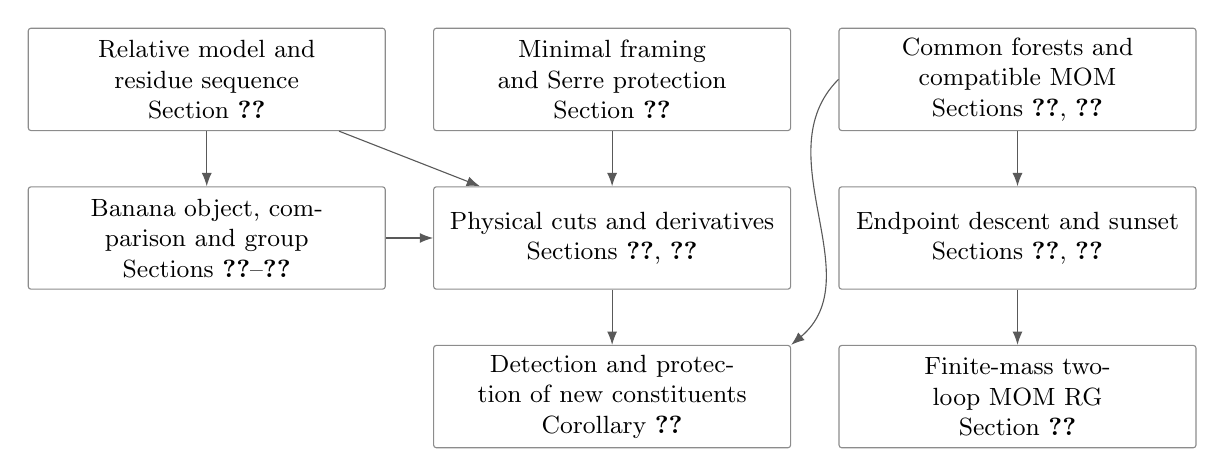
\begin{tikzpicture}[node distance=7mm and 6mm,box/.style={draw=black!45,rounded corners=1pt,align=center,font=\small,text width=43mm,minimum height=13mm},arr/.style={-Latex,draw=black!65}]
\node[box] (geo) {Relative model and residue sequence\\Section~\ref{ch:unified}};
\node[box,right=of geo] (alg) {Minimal framing and Serre protection\\Section~\ref{ch:unified}};
\node[box,right=of alg] (ren) {Common forests and compatible MOM\\Sections~\ref{ch:zero}, \ref{ch:finitemom}};
\node[box,below=of geo] (ban) {Banana object, comparison and group\\Sections~\ref{ch:core}--\ref{ch:fixed}};
\node[box,below=of alg] (cut) {Physical cuts and derivatives\\Sections~\ref{ch:connection}, \ref{ch:cut}};
\node[box,below=of ren] (sun) {Endpoint descent and sunset\\Sections~\ref{ch:descent}, \ref{ch:sunsetjet}};
\node[box,below=of cut] (protect) {Detection and protection of new constituents\\Corollary~\ref{unified:cor:prediction}};
\node[box,below=of sun] (rg) {Finite-mass two-loop MOM RG\\Section~\ref{ch:momrg}};
\draw[arr] (geo)--(ban);\draw[arr] (geo)--(cut);
\draw[arr] (alg)--(cut);\draw[arr] (cut)--(protect);
\draw[arr] (ren.west) to[out=225,in=40] (protect.north east);
\draw[arr] (ren)--(sun);\draw[arr] (sun)--(rg);
\draw[arr] (ban)--(cut);
\end{tikzpicture}
\caption{Principal proof dependencies. Arrows indicate inputs used. Certification at the fixed banana fiber and four-dimensional two-loop MOM form independent chains of examples. They share a structural method; the latter does not require the rank-eight mixed banana object.}
\label{fig:dependencies}
\end{figure}

\paragraph{Categories and normalization.}\label{sec:notation}
We retain the ground field $k\subset\mathbb C$ and its chosen embedding throughout, and use rational coefficients for motives. The weight of $\mathbb Q(j)$ is $-2j$, with standard Tate period $(2\pi i)^j$. Physical chains are written homologically. Geometric residues are usually written first in cohomology and then dualized. In families we use geometrically arising admissible variations of mixed Hodge structure and their subquotients; at fixed algebraic fibers we use Nori objects. Compatibility of the six operations and realizations is taken from the published results of Tubach\cite{tubach}, and the 1-motivic quotient from Ayoub--Barbieri-Viale\cite{abv}. Appendix~\ref{app:inputs} restates these foundational inputs and explains how they are used.

We do not assume that the numerical period map is injective. Vanishing at a single numerical point, vanishing identically as a function of the family parameter, vanishing as a formal period, and annihilation of a subobject by a functional require different arguments. The finite certificates for the specified banana fiber are listed as inputs. Ordinary decimals and rigorous intervals for the scattering benchmark are distinguished explicitly. A reader may begin with Section~\ref{ch:unified} and the banana example, then follow Figure~\ref{fig:dependencies} to the relevant operations.


\section{A unified structural framework}\label{ch:unified}
This section begins with minimal framings. We first prove stability under the addition of background periods, then place geometric residues and physical chains within a common system of upper and lower bounds. Finally, the connection turns these structural relations into inhomogeneous differential equations.

\begingroup
\providecommand{\Q}{\mathbb Q}\providecommand{\cC}{\mathcal C}
\providecommand{\cS}{\mathcal S}\providecommand{\dR}{\mathrm{dR}}
\providecommand{\rk}{\operatorname{rk}}\providecommand{\im}{\operatorname{im}}
\subsection{Framed objects in the specified category}
\subsubsection{Input and classification output}
The input is
\[
 \mathfrak P=(G,D,\nu,\mu,\kappa,N,\sigma,k,R,\mathcal O),
\]
consisting, respectively, of the graph, dimension, propagator powers, masses, kinematics, numerator, chain, base field, subtraction scheme, and observable.
The primary output is a framed object in the specified category, rather than a single ``MPL/elliptic/K3'' label determined solely by the edge list.

In the constructed rational Nori category or the explicitly specified realization category $\cC$, we use the homological convention:
$E$ carries the chain $\sigma\in E_B$, and the form defines a functional $\lambda\in E_{\dR}^{\vee}$.
The de Rham coefficients may lie in a number field $k$, but subobjects are still taken in the original category, retaining the descent conditions.
Write the period as $p=[E,\sigma,\lambda]$; this notation suppresses the duality with the cohomological convention. Define
\[
 R_\sigma=\bigcap_{\sigma\in J_B}J,\quad
 I_\lambda=\sum_{\lambda|J_{\dR}=0}J,\quad
 M(p)=R_\sigma/(R_\sigma\cap I_\lambda).
\]
Finite length and exactness of the realizations ensure existence. Independence of the presentation of the minimal matrix-coefficient object is a classical result
\cite[\S2.4]{brownperiods}, not a new definition or theorem of this paper.

A complete classification comprises three sets of data: simple constituents, weights, Hodge numbers, polarizations, and arithmetic descent;
the gluing between layers in the specified category and the compatibility relations among multiple layers; and the framing, together with the source, target, and actual morphism for each operation.
Listing only simple constituents misses Kummer and regulator data; listing only adjacent $\operatorname{Ext}^1$
classes need not determine an object with several layers. The precise output remains a filtered and framed object in the specified category, or an equivalent presentation whose validity has been proved.

\subsubsection{The levels of meaning in the structural table}
\begin{center}\small
\begin{tabular}{p{24mm}p{47mm}p{72mm}}
\toprule Name&Level of the valid conclusion&What the name alone does not imply\\\midrule
MPL&An iterated-integral representation with specified letters, paths, and endpoints&Values at arbitrary algebraic letters are MZVs\\
MZV&Constants with a specified normalization and their formal periods&All mixed Tate periods belong to this subclass\\
mixed Tate&All constituents of the object in the specified category are the corresponding Tate objects&Extensions split, or a specified MPL expression is automatic\\
Elliptic/higher genus&The $H^1$ of a curve and its visible constituents&Equal genus means the same object, or all factors are physically visible\\
K3&A specified transcendental $H^2$ and its gluing to the boundary&Every rank-six equation is K3, or the entire period has only pure layers\\
Higher-dimensional CY&Specified geometry, degree, and a cohomological certificate&Every differential equation of high order is CY\\
Kummer&Units and their extension classes in the specified category&Base fields, branches, and comparison data are unnecessary\\\bottomrule
\end{tabular}
\end{center}
For example, the Kummer extension associated with the mass unit $2$ and a specified MZV endpoint object have different arithmetic inputs.
This observation requires no assertion of the unknown algebraic independence of $\log2$ from any collection of ordinary numerical values.
The table specifies the meaning of the output; sufficient criteria must still come from the geometry itself.


\subsection{Additive stability under background periods}
\subsubsection{The background subcategory and the appropriate quotient}
Let $\cS\subset\cC$ be a Serre subcategory, that is, one closed under subobjects, quotients, and extensions.
Write $\pi:\cC\to\cC/\cS$ for the exact quotient functor, using the standard existence theorem
\cite[Tag 02MS]{stacks}. This quotient compares only the constituents lying beyond the background structure;
in general it is not a category of motives equipped with a fiber functor.

If the background contains the unit object, it cannot also be required to be a
``tensor ideal'' closed under tensoring with arbitrary ambient objects: $1\otimes E=E$ would force it to equal all of $\cC$.
Below we use the \emph{Serre closure} of a given background tensor subcategory, without this additional requirement.
In a finite-length category, this closure consists precisely of the objects all of whose simple constituents belong to the background list.

\begin{theorem}[Additive stability under background periods]\label{unified:thm:addition}
Let $p$ be a formal period in the specified category, let $\ell=[L,\tau,\eta]$ with $L\in\cS$,
and let $q=p+\ell$. Then
\begin{equation}\label{unified:eq:quotient}
 \pi M(q)\simeq\pi M(p).
\end{equation}
For every simple object $S$ not belonging to $\cS$,
\[
 [M(q):S]=[M(p):S].
\]
There is also a rank bound depending on the chosen carrier of the perturbation:
\[
 |\rk M(q)-\rk M(p)|\leq\rk L .
\]
Neither the complex values of $p,\ell$ nor injectivity of the period map is needed.
\end{theorem}
\begin{proof}
Choose the minimal framing $(\sigma,\lambda)$ of $P=M(p)$.
Thus $\sigma$ generates $P$, and $P$ has no nonzero subobject annihilated by $\lambda$.
On $P\oplus L$, the period $q$ is represented by the chain $(\sigma,\tau)$ and functional $(\lambda,\eta)$.
Let $R$ be the subobject generated by this chain, and let $I\subset R$ be the largest subobject annihilated by this functional.
Then $M(q)=R/I$.

The image of the projection $R\to P$ carries $\sigma$, so the projection is surjective. Its kernel $K$ is a subobject of $L$,
hence $K\in\cS$. On the other hand,
\[
 I\cap(P\oplus0)=0,
\]
since a nonzero intersection would be a subobject of $P$ in the specified category on which $\lambda$ vanishes, contradicting minimality.
The projection $I\to L$ is therefore injective, so $I\in\cS$. The two short exact sequences
\[
 0\to K\to R\to P\to0,\qquad
 0\to I\to R\to M(q)\to0
\]
become isomorphisms under $\pi$, proving \eqref{unified:eq:quotient}.
Additivity of constituent multiplicities gives
$[M(q):S]-[P:S]=[K:S]-[I:S]$;
for $S$ outside the background, the right-hand side is zero.
The rank difference is $\rk K-\rk I$, and both ranks lie between $0$ and $\rk L$, proving the rank bound.
All these are subquotients in the specified category, rather than objects guessed after adding numerical values.
\end{proof}

This conclusion is stronger than the assertion that ``the same tensor category is generated after adjoining the background'':
that assertion does not determine how many times a new simple factor occurs in an object, whereas the theorem preserves its exact multiplicity.
The background may represent lower-loop graphs, known boundary contributions, or other allowed structures,
but one must first prove that the perturbation is indeed carried by an object of that background in the specified category.

\subsubsection{Why mixed extensions must still be studied separately}
If $\cS$ consists of all objects whose constituents are Tate, both a nonsplit Kummer object and its split replacement map to zero.
For example, $p=\log^{\mathfrak m}2$ and $\ell=-p$ allow $q=0$:
both are zero in the quotient, although their original minimal objects differ.
Thus the quotient does not replace regulators, units, or the full coaction;
it answers precisely whether additive changes can remove new structure outside the background.
A complete classification must retain both these stable pure constituents and the gluing in the specified category.


\subsection{Protection of new constituents under anchored renormalization}
\subsubsection{The established graph class and the lower-loop background}
We work with the graph class established in this paper: positive-mass Euclidean $D=4$ graphs with unit propagator powers and at most logarithmic divergences,
using the constructed zero-momentum or compatible algebraic nonzero MOM reference schemes.
Let $a,b$ be two schemes, let $h_G=h>0$, and fix a common physical anchor $\kappa_*$:
\[
 p_a=\widehat\Phi_a^{\mathfrak m}(G;\kappa,\kappa_*)
 =\Phi_a^{\mathfrak m}(G;\kappa)-\Phi_a^{\mathfrak m}(G;\kappa_*).
\]
The current point, anchor, and reference data lie in the established positive-mass algebraic Euclidean range.
When the base field or algebraic normalization changes, the required arithmetic objects must be explicitly included in the background.

The theorem on finite scheme changes in the specified category in Section~\ref{ch:finitemom} gives
\begin{equation}\label{unified:eq:forest}
 p_b-p_a=\sum_{\varnothing\ne\gamma\subsetneq G}
 g_{ba}^{\mathfrak m}(\gamma)\,
 \widehat\Phi_a^{\mathfrak m}
 (G/\gamma;\pi_\gamma\kappa,\pi_\gamma\kappa_*).
\end{equation}
The subgraph may be a disconnected union allowed by the forest coproduct, and every factor comes from a carrier of strictly lower loop order in the specified category.
For the classical forest background see \cite{bk2012}; for the lift to periods in the specified category and the comparison with the cutoff physical integral, see Sections~\ref{ch:zero} and~\ref{ch:finitemom}.

Let $\mathcal B_{<G}$ be the full tensor subcategory generated by all strictly lower-loop carriers required for the transformations in this section,
including the finite closure under subgraphs and contractions, the reference points, and evaluations at the current point and anchor,
together with the required Tate factors. Let $\cS_{<G}$ be its Serre closure in the common ambient category.
``New geometry'' is always relative to this explicit background; it cannot be specified informally by loop order alone.

\begin{theorem}[Scheme invariance of new structure]\label{unified:thm:ren}
In the range specified above,
\[
 \pi_{<G}M(p_a)\simeq\pi_{<G}M(p_b).
\]
Every simple object $S$ outside the background has the same multiplicity in both objects.
If the entire lower-loop background is mixed Tate and the anchored minimal object in one scheme contains a non-Tate simple constituent,
then the other scheme still contains that constituent with the same multiplicity.
\end{theorem}
\begin{proof}
Each product in \eqref{unified:eq:forest} is carried by the tensor product of its carriers in the specified category,
and the finite sum is carried by the direct sum $L$ of these tensor products.
Thus $L\in\mathcal B_{<G}\subset\cS_{<G}$.
Apply Theorem~\ref{unified:thm:addition}.
If the lower-loop objects are all mixed Tate, their tensor products, subquotients, and extensions still have only Tate constituents,
so every non-Tate simple factor lies outside the background.
\end{proof}

This directly connects the structural table with physical operations: once geometry proves that a new pure factor enters the specified framing,
allowed changes of anchored scheme cannot turn it into background structure.
The argument neither evaluates the full integral nor misinterprets locality as the disappearance of all constants.

\subsubsection{The anchor condition and the distinction from physical summation}
The unanchored difference contains the whole-graph constant $g_{ba}(G)$,
which may involve reference periods of the same loop order and cannot be assigned to the lower-loop background.
Even a primitive graph satisfies
\[
 \Phi_b(G;\kappa)-\Phi_a(G;\kappa)
 =\Phi_0(G;\rho_a)-\Phi_0(G;\rho_b).
\]
A bubble vanishes at its own subtraction point, but may become strictly nonzero there after changing the reference point;
thus the minimal object at an isolated point can change from zero to nonzero.
Changing a physical numerator or the full sum of graphs is also distinct from changing the scheme:
such changes may produce genuine cancellation within the same new geometry, and the theorem does not rule this out.


\subsection{Geometric upper bounds and physical lower bounds}
\subsubsection{Upper bounds from finitely many operations in the specified category}
\begin{proposition}[Structural upper bound]\label{unified:prop:upper}
Given finitely many seed objects in the specified category, allow finite direct sums, tensor products, duals, Tate twists,
kernels, images, and cokernels of actual morphisms, and specified short exact sequences.
If their constituents belong to a background class closed under subquotients, tensor products, duals, and extensions,
then the constituents of every output and every physical minimal object remain in that class.
\end{proposition}
\begin{proof}
Multiplicities are additive in direct sums and exact sequences, and passing to subquotients only removes constituents.
Tensor products are exact on finite-length filtrations, with successive quotients given by tensor products of constituents.
Taking their constituents, and including duals and twists, proves the claim by induction.
The final physical minimization is itself passage to a subquotient.
\end{proof}
Extensions can still add regulator data and unipotent depth.
Cuts, contractions, and Gauss--Manin derivatives are not all endomorphisms of a fixed object:
new geometry requires its own object and comparison in the specified category, rather than an inference from formal resemblance.

\subsubsection{Chain-compatible cuts force lower bounds}
Suppose an actual tube morphism $f:C\to E$ already incorporates the correct Tate twist and orientation.
The cut functional is $f^*\lambda$, the cut chain is $\gamma$,
and its image generates $R_{f\gamma}$ in $E$.
\begin{proposition}[Physical protection of a cut]\label{unified:prop:lower}
If $R_{f\gamma}\subset R_\sigma$, there is an injection in the specified category
\[
 M([C,\gamma,f^*\lambda])\hookrightarrow M([E,\sigma,\lambda]).
\]
Hence every simple constituent of the cut minimal object occurs in the physical minimal object with at least the same multiplicity.
\end{proposition}
\begin{proof}
The framing relation in the specified category identifies the left-hand side with
$R_{f\gamma}/(R_{f\gamma}\cap I_\lambda)$,
which injects into $R_\sigma/(R_\sigma\cap I_\lambda)$ by the assumed inclusion.
\end{proof}
The condition is automatic when the original chain cyclically generates $E$.
Otherwise, a nonzero generalized cut may come from a direction not excited by the original chain, and certifies only the ambient geometry.
For a full physical sum, one must first form the total functional and then test the cut; interference cannot be ignored graph by graph.

\begin{corollary}[A certificate of non-eliminability without evaluating the full integral]\label{unified:cor:prediction}
Suppose a geometric upper bound and framing have been constructed, a cut satisfies the chain condition above,
the cut minimal object contains a simple factor $S$, and $S\notin\cS_{<G}$.
Then the physical output must contain $S$, and retains it in every anchored scheme covered by Theorem~\ref{unified:thm:ren}.
If the multiplicity of $S$ in the upper bound equals the lower bound supplied by the cut, that multiplicity is determined exactly.
\end{corollary}
\begin{proof}
Apply Proposition~\ref{unified:prop:lower} and Theorem~\ref{unified:thm:ren} in turn, then compare the integer multiplicities between the two bounds.
\end{proof}
This is the main criterion that can be used throughout the paper. Every premise requires evidence:
unproved chain generation or regulator nonvanishing cannot be hidden inside ``automatic compilation.''
The corresponding inputs for the specified banana fiber have independent proofs.
For general graphs, one may stop at an upper bound or a conditional lower bound, but the strength of the output must be stated.

\subsubsection{Verifying the chain condition by physical variation: families and fixed fibers}
Let $S$ be a connected smooth parameter curve, and let $\mathcal E$ be the already constructed variation
homologically dual to relative cohomology, with a rational Betti local system and an algebraic de Rham connection.
Below, subobjects are taken in a finite-length category of variations whose Betti realizations are local systems;
one may use geometrically arising admissible variations of mixed Hodge structure and their subquotients.
Results at the level of realizations do not assert the existence of unconstructed Nori morphisms over a family.
Fix a base point $s_*$, a chain $\sigma$, and a single-valued algebraic functional $\lambda$.
Write $R_\sigma^{\rm var}$ for the smallest subvariation containing $\sigma$,
and $I_\lambda^{\rm var}$ for the largest subvariation identically annihilated by $\lambda$.

\begin{theorem}[Cut protection from physical variation]\label{unified:thm:variation}
Suppose an actual tube morphism $f:\mathcal C\to\mathcal E$ and a path $\ell$ satisfy
\[
 (T_\ell-1)\sigma=c\,f_B\gamma,\qquad c\in\Q^\times.
\]
Then, in the category of variations,
\[
 M_{\rm var}(\mathcal C;\gamma,f^*\lambda)
 \hookrightarrow M_{\rm var}(\mathcal E;\sigma,\lambda).
\]
If the image of the actual tube morphism contains a subvariation $\mathcal A$ with irreducible Betti local system,
and $f_B\gamma\in\mathcal A_{s_*}$ is nonzero with $\lambda|_{\mathcal A}\not\equiv0$,
then $\mathcal A$ injects into the physical minimal variation.
\end{theorem}
\begin{proof}
The Betti fiber of $R_\sigma^{\rm var}$ is preserved by all monodromy, so it contains both $\sigma$
and $T_\ell\sigma$, and hence $f_B\gamma$. Minimality gives
$R_{f\gamma}^{\rm var}\subset R_\sigma^{\rm var}$; apply Proposition~\ref{unified:prop:lower}.
For the second assertion, the local system of $\mathcal A\cap R_\sigma^{\rm var}$ is nonzero,
so irreducibility forces this intersection to equal $\mathcal A$. Meanwhile,
$\mathcal A\cap I_\lambda^{\rm var}$ is either zero or the whole subvariation,
and the nonzero functional excludes the latter possibility.
\end{proof}
This settles one substantive condition on chain inclusion in a family, but does not remove the need to establish the tube comparison and intersection number.
If the variation is a sum of several cuts rather than a single tube period, one must first take the minimal object of the total cut;
the individual terms cannot each be treated as already protected.

\begin{proposition}[A differential-order lower bound without evaluating the full integral]\label{unified:prop:order}
Let $F$ be a physical period function, and suppose one of its variations equals a nonzero cut function $c\,g$.
If the solution space $W$ spanned by all analytic continuations of $g$ is irreducible and has dimension $r$,
then every scalar homogeneous operator with single-valued meromorphic coefficients satisfying $LF=0$ has
$\operatorname{ord}L\ge r$.
If $W$ is defined by a monic operator $L_{\rm cut}$ of order $r$ in $K[\partial_s]$,
then every such $L\in K[\partial_s]$ satisfies
\[
 L=A\,L_{\rm cut}.
\]
\end{proposition}
\begin{proof}
Analytic continuation commutes with operators having single-valued coefficients, so $L$ annihilates the variation of $F$ and all its continuations.
It therefore annihilates the entire $r$-dimensional space $W$; at an ordinary point, the local solution space of an equation of order $m$ has dimension at most $m$.
Right division of $L$ by $L_{\rm cut}$ leaves a remainder of order less than $r$ that still annihilates $W$, so the remainder must vanish.
\end{proof}
An irreducible cut local system and a nonzero algebraic functional usually supply the dimension $r$ here:
the kernel of the map from flat vectors to period functions is monodromy invariant, and irreducibility forces it to vanish.
If algebraic coefficients are allowed, irreducibility must persist on the corresponding finite cover;
this holds when the connected geometric monodromy group already acts irreducibly.

\textbf{The limitation at a fixed fiber.}
In general, $T_\ell$ is not a Hodge endomorphism of $(\mathcal E_{s_*},F^\bullet,W_\bullet)$.
Thus $M_{\rm var}$ in this theorem cannot be replaced by $M$ at an arbitrary specified point.
For example, for the established fixed banana fiber with $\operatorname{End}_{\rm Hdg}T=\Q$,
a nonscalar nodal reflection is not a morphism of the fixed Hodge structure.
Rank-eight minimality at the specified point $s=-64$ still rests on the original regulator and group arguments;
it is not reproved by this differential lower bound.
More generally, the accidental vanishing of a numerical period at one fiber does not erase the solution space of a nonzero function of the family.

\subsubsection{A geometric physical entry point at arbitrary loop order: the normal threshold of the two-dimensional banana}
Let $h\ge2$, $n=h-1$, $m_i>0$, and $\mu_i=m_i^2$.
Use the explicit positive-parameter normalization
\[
 I_h(s)=\int_{\alpha_i>0,\ \alpha_h=1}
 \frac{d\alpha_1\cdots d\alpha_n}
 {(\sum_i\mu_i\alpha_i)U_h-s\prod_i\alpha_i}.
\]
This omits the external $\pi,i$ factors from the momentum-space measure;
for $h=4$, the positive orientation agrees with the Euclidean parametric period used in this paper.
In this chart, set $y_i=\log(m_i\alpha_i/m_h)$ and $y_h=0$. Then
\[
 I_h(s)=\int_{\mathbb R^n}\frac{dy_1\cdots dy_n}{f(y)-s},
 \qquad
 f(y)=\Big(\sum_{i=1}^h m_i e^{y_i}\Big)
       \Big(\sum_{i=1}^h m_i e^{-y_i}\Big).
\]
Let $M=\sum_i m_i$ and $s_0=M^2$.

\begin{theorem}[Threshold nonvanishing of the positive physical chain]\label{unified:thm:threshold}
The function $I_h$ is holomorphic on $\mathbb C\setminus[s_0,\infty)$.
The function $f$ is strictly convex and proper, with unique minimum at $y=0$ and minimum value $s_0$.
For $t>s_0$, the positively oriented boundary-value difference is
\[
 I_h(t+i0)-I_h(t-i0)=2\pi i\,\rho_h(t),\qquad
 \rho_h(t)=\int_{\mathbb R^n}\delta(f(y)-t)\,dy>0.
\]
As $\varepsilon\downarrow0$,
\[
 \rho_h(s_0+\varepsilon)=
 \frac{\pi^{n/2}}
 {\Gamma(n/2)\,M^{(h-2)/2}\sqrt{\prod_i m_i}}\,
 \varepsilon^{(h-3)/2}\bigl(1+O(\varepsilon)\bigr).
 \tag{T}
\]
The local chain variation is a single tube over the normal Morse vanishing sphere, with orientation fixed by the formula above
and intersection number of absolute value one. In particular, the physical branch does excite this cut.
\end{theorem}
\begin{proof}
Expand
\[
 f=\sum_i m_i^2+2\sum_{i<j}m_i m_j\cosh(y_i-y_j).
\]
In any nonzero direction $v$ with $v_h=0$, the Hessian quadratic form is
$2\sum_{i<j}m_i m_j\cosh(y_i-y_j)(v_i-v_j)^2>0$.
All differences vanish simultaneously only at $y=0$, and Cauchy--Schwarz gives the minimum value.
If $R=\max_i y_i-\min_i y_i$, then
$f\ge m_{\min}^2e^R$ and $R\ge\|y\|_\infty$.
Thus $f$ is proper, and the integral has an exponentially integrable bound at infinity.
For any compact set of $s$ avoiding the cut, the denominator has a uniform relative lower bound.
Arbitrarily many $s$-derivatives may therefore be taken under the integral, proving holomorphicity.

Strict convexity implies that each compact level set with $t>s_0$ contains no critical point.
Push the positive measure forward using the coarea formula, then take the one-dimensional Cauchy boundary values of $1/(u-t\mp i0)$
to obtain the jump formula. The level set is nonempty and its density is everywhere positive, so $\rho_h(t)>0$.
This is a direct proof for the present parametric integral; it does not assume a multiloop Cutkosky theorem in arbitrary dimension.

At the minimum, put $m=(m_1,\ldots,m_n)^t$. Then
\[
 f-s_0=y^tAy+O(\|y\|^4),\quad
 A=M\,\operatorname{diag}(m_1,\ldots,m_n)-mm^t,
 \quad \det A=M^{h-2}\prod_{i=1}^h m_i.
\]
The matrix determinant lemma gives the last equality.
Real-analytic Morse coordinates reduce $f-s_0$ to $\|u\|^2$,
and the volume density at the origin is $(\det A)^{-1/2}$.
Spherical averaging removes every odd-degree term, so the leading term is
\[
 (\det A)^{-1/2}
 \int_{\mathbb R^n}\delta(\|u\|^2-\varepsilon)\,du
 =\frac{\pi^{n/2}\varepsilon^{n/2-1}}
 {\Gamma(n/2)\sqrt{\det A}},
\]
with relative error $O(\varepsilon)$, including when $n=1$.

Finally, take a small ball about the minimum. Outside it, $f-s_0$ has a positive lower bound,
so the exterior integral is holomorphic near $s_0$ and cannot contribute to this local variation.
Inside the ball, the real chain intersects the local cell dual to the Morse vanishing cell transversely exactly once.
Alternatively, bypassing the unique simple pole in the radial variable directly gives a single Cauchy tube.
Its positive residue density is exactly the one above, so the multiplicity is not an undetermined integer.
For the classical local-tube and Picard--Lefschetz interpretation, compare \cite[\S2.3]{muhlbauer}.
\end{proof}
The positive $y$-chart corresponds to the future-directed on-shell branch, and the light-cone and parametric cut varieties have already been identified.
This therefore establishes physical excitation at the normal threshold.
It neither computes every anomalous threshold or global contour nor completes all comparisons of momentum-space measures.

\begin{corollary}[From the threshold to an irreducible geometric core]\label{unified:cor:banana-threshold}
If the compact cut period of this normal vanishing sphere belongs to a pure local system of dimension $r$ whose irreducibility has been proved,
then a scalar homogeneous differential equation for $I_h$ has order at least $r$ and contains the corresponding cut operator as a right factor.
When the tube morphism of variations has been constructed in the specified category, the object protection of Theorem~\ref{unified:thm:variation} also follows.
\end{corollary}
\begin{proof}
Formula~(T) ensures that the cut function is nonzero, and irreducibility makes its continuations generate the entire pure core.
Apply Proposition~\ref{unified:prop:order} and Theorem~\ref{unified:thm:variation}.
\end{proof}
For $h=3$, an irreducible elliptic variation gives $r=2$;
for $h=4$ along the $m=(1,2,4,8)$ ray, the established pure monodromy group gives $r=6$.
Both conclusions are lower bounds for the physical function; they do not make the ranks of the full mixed objects or the homogeneous orders equal to $2,6$, respectively.
The same threshold formula holds for $h>4$, but the threshold exponent alone does not establish irreducibility of a CY core.


\subsection{Scope of the structural criteria}
The following table distinguishes full integrals, maximal cuts, and finite coefficient expansions, without conflating their ranks.
\begin{center}\small
\begin{longtable}{>{\raggedright\arraybackslash}p{29mm}>{\raggedright\arraybackslash}p{51mm}>{\raggedright\arraybackslash}p{61mm}}
\toprule Input class&Established conclusions&Current limitations\\\midrule\endfirsthead
\toprule Input class&Established conclusions&Current limitations\\\midrule\endhead
Unit-power scalar graphs with generically independent energy roots&
Necessary and sufficient dual-critical support criterion; parity compression of edge bundles&
Character support is not a motivic direct sum\\
Nondegenerate cycle-star graphs&
Geometric double covers, character hosts, all characters for the scalar integral, and numerator rules&
The three-layer boundary of the compact cut has been constructed; comparison of the full graph with the curve, the chain, and isogenous specializations require separate analysis\\
Positive-mass one-loop triangles/boxes&
Full mixed Artin--Tate carriers; ranks 7/8 in general position and a quadratic-character table&
The full parametric chain and algebraic source have been incorporated; carrier rank is not physical rank before minimization\\
Accepted Euler/MZV graph rules&
The finite Euler expansion and formal MZV comodule from the original v2&
An analytic graph identity does not automatically give an isomorphism of Nori minimal objects for the original higher-dimensional graph\\
Two-dimensional four-propagator banana&
Constructed relative object, K3, mass Kummer data, and regulator; minimal rank eight, coaction, and group at the specified point&
The specified point, a very general four-parameter point, and the equal-mass stratum are treated separately\\
Two-dimensional positive-mass banana for arbitrary $h$&
Unique pinch at the normal threshold, intersection number of absolute value one, and a nonzero leading cut term; an irreducible core gives a physical differential lower bound&
Irreducibility of higher-dimensional pure cores requires a separate proof; not all anomalous thresholds are covered\\
Residue-free relative curve periods in the specified category&
Endpoints give algebraic inhomogeneous sources; under cut protection, the minimal homogeneous order is $r$ or $r+1$&
Primitives, moving endpoints, and the comparison in the specified category are indispensable; motivic rank at a fixed point requires separate analysis\\
Positive-mass logarithmic graphs and compatible MOM&
Constructed forests and endpoints; preservation of new structure under scheme changes in this section&
General powers, IR divergences, and arbitrary schemes are excluded\\
Four-dimensional sunset and two-loop $\phi^4$&
Constructed two-point carrier and finite-order RG output in the same scheme&
These are physical examples; extending lists of low-order coefficients does not replace the overall classification\\
Single-coupling MS-type RG&
Invertibility between local coefficients and critical expansions, and preservation of structure, under the stated conditions&
The scheme and thermal-direction conditions remain essential; MOM masses cannot be substituted mechanically\\
Higher-dimensional CY and general mixed graphs&
Unified rules for geometric upper bounds, cut lower bounds, and extension checks&
No complete decision procedure yet covers arbitrary edge lists\\
Serially subdivided sunrise, in two dimensions with positive masses and zero internal momentum injection &
Descent of the full period in the specified category to a direct sum of endpoint sunrises; at most one elliptic constituent per endpoint &
For distinct masses and separated normal thresholds, each elliptic constituent not removed by the numerator occurs exactly once; at most one survives when equal masses coalesce. \otherref{feynman_periods_supplement_en}{Supplement S1.1}.\\
Four-edge two-loop three-point graph, allowing nonzero internal injection &
A rational pole surface and two elliptic boundary faces; non-AT semisimple rank four for the full relative carrier &
The single scalar functional contains exactly the two elliptic cores; each contraction numerator selects one. An explicit slice has homogeneous order at least four; absolute annihilation can leave an elliptic source. Sections~\ref{unified:sec:boundaryelliptic}--\ref{unified:sec:scalarboundary}.\\
Physical sums of graphs and threshold backgrounds&
Equality of the ranks of the full variation operator and its semisimple associated graded; geometric forest carriers extend across the chosen degeneration component.&
The rank of continued jumps gives multiplicities in the function core; multiplicities outside the background are protected by scheme comparison. A crossing combination of three graphs retains three elliptic channels, with non-AT rank 6--12. \otherref{feynman_periods_supplement_en}{Supplement S1.2}.\\
Three-path theta subdivision families with zero internal injection&
Relative Stokes descent in the specified category; each mass triple gives an elliptic carrier upper bound.&
Under threshold separation, every nonzero entry of the numerator grid contributes one elliptic core; the rank $2r_1r_2r_3$ can be unbounded. For the finite-skeleton bound and its hypotheses, see \otherref{feynman_periods_supplement_en}{Supplement S1.3}.\\
\bottomrule
\end{longtable}
\end{center}
Different entry points must be joined by comparisons in the specified category; the ambient object cannot replace the minimal physical object.
The table rests on the retained internal proofs and original material, which are not presented as externally peer-reviewed results.


\subsection{The residue image, a fixed ambient object, and inhomogeneous sources}
\label{unified:sec:pencil}
\subsubsection{The fixed ambient geometry is a required input}
The curve rules of Section~\ref{ch:graph} require the full period to have been identified as a relative curve period.
For a general graph for which this step is incomplete, one may work directly with its higher-dimensional parametric model.
Let $k\subset\mathbb C$ be a field of characteristic zero, let $X/k$ be smooth,
and let $B\subset X$ be a fixed simple normal crossings boundary.
The fixed pole locus has already been removed from $X$.
Let $Y_s\subset X$ be a family of smooth divisors over an algebraic parameter curve $S$,
transverse to every intersection stratum of $B$.
Shrink $S$ if necessary so that the relative cohomology groups in use form locally free objects with Gauss--Manin connection.
Both the relative form and the physical chain must belong to the following geometric model:
\[
 J=H^n(X,B),\qquad
 M_s=H^n(X\setminus Y_s,B\setminus Y_s),\qquad
 C_s=H^{n-1}(Y_s,B\cap Y_s)(-1).
\]
Here $M_s$ follows the cohomological convention, and the preceding minimal physical object is carried by $E_s=M_s^\vee$.
The object $J$ comes from fixed geometry; this does not make $J$ automatically Tate.
The class $\omega_s\in(M_s)_{\dR}$ is algebraic and relative,
$\sigma_s\in(M_s)_B^\vee$ is flat on a simply connected parameter open set,
and $I(s)=\langle\sigma_s,\omega_s\rangle$.
Terms arising from the moving physical boundary are already included in the relative Gauss--Manin connection.

\begin{theorem}[Exact separation of the residue image from the ambient background]\label{unified:thm:pencil-separation}
In the geometric model above, there is an exact segment compatible with the connections:
\begin{equation}\label{unified:eq:pencil-gysin}
 J\longrightarrow M_s\xrightarrow{\mathrm{res}}C_s
       \longrightarrow H^{n+1}(X,B).
\end{equation}
Let $K_s=\ker(\mathrm{res})$ and $A_s=\im(\mathrm{res})$.
Then $K_s$ is a quotient of $J$, $A_s$ is a subobject of $C_s$, and
\[
 0\longrightarrow K_s\longrightarrow M_s\longrightarrow A_s
 \longrightarrow0.
\]
At each specified algebraic fiber, take a Serre background $\cS$ containing every simple constituent of $J$. Then
\[
 \pi M_s\simeq\pi A_s.
\]
Thus the simple constituents of the full model outside this background, with their multiplicities, are exactly those of the residue image in the specified category.
For the physical minimal object, multiplicities outside the dual Serre background $\cS^\vee$ are at most the corresponding multiplicities in $A_s^\vee$;
if an actual cut and the physical framing additionally supply a lower bound attaining this upper bound, these multiplicities are determined exactly.
\end{theorem}
\begin{proof}
Write the localization triangle for $Y_s\subset X$. Codimension-one purity gives
$R\Gamma(Y_s)(-1)[-2]\to R\Gamma(X)\to
R\Gamma(X\setminus Y_s)\to$.
Write the same triangle on every intersection stratum of $B$.
Transverse base change makes these triangles compatible with restriction. Taking the finite intersection complex and the relative mapping fiber gives
\[
 R\Gamma(Y_s,B\cap Y_s)(-1)[-2]\longrightarrow
 R\Gamma(X,B)\longrightarrow
 R\Gamma(X\setminus Y_s,B\setminus Y_s)\longrightarrow.
\]
Taking cohomology in degree $n$ yields \eqref{unified:eq:pencil-gysin}.
The six operations in the specified category and their Nori realizations give fiberwise morphisms, while naturality of Gauss--Manin gives compatibility with the connections in the family.
No general ``category of Nori variations'' is additionally assumed to have been constructed.
Exactness makes $K_s$ a quotient of $J$; the Serre quotient annihilates $K_s$, giving the isomorphism.
After dualizing, $E_s$ is an extension of $A_s^\vee$ and $K_s^\vee$,
and the minimal physical object is a subquotient of $E_s$. Thus the multiplicity of each simple factor outside $\cS^\vee$ is bounded by the corresponding upper bound.
When the bound is attained, finite length gives the final assertion.
\end{proof}

This separates two easily confused issues: $C_s$ may be larger than the residue image $A_s$;
even when $A_s$ is completely known, the physical framing may see only part of it.
If $J$ is mixed Tate, all non-Tate simple constituents come from the \emph{relative} residue object $C_s$.
But $C_s$ itself still includes boundary data and is not automatically the compact pure cut core.
Physical variation in a family can give lower bounds at the level of connections or variations;
these cannot be called Nori lower bounds at a specified fiber without a comparison.

\subsubsection{Inhomogeneous sources need not be inferred from the full integral}
Take $K=k(S)$ with the derivation $\partial$ associated with a nonconstant local parameter,
and assume its constant field is $k$.
Fix a $k$-basis $e_1,\ldots,e_d$ of $J_{\dR}$, where $d=\dim J_{\dR}$.

\begin{theorem}[A fixed ambient source after annihilation of the residue class]\label{unified:thm:ambient-source}
Suppose $L\in K[\partial]$ satisfies
$L\,\mathrm{res}(\omega)=0$, where zero means vanishing of the de Rham class in the specified category.
Then there exist $a_j\in K$ such that
\begin{equation}\label{unified:eq:ambient-source}
 L I(s)=\sum_{j=1}^d a_j(s)P_j,\qquad
 P_j=\langle\tau,e_j\rangle,
\end{equation}
where $\tau$ is the image of $\sigma_s$ in the fixed pair $(X,B)$ and is independent of $s$.
Each $P_j$ is a period of the fixed ambient object $J$.
The same identity holds for the corresponding formal periods in the specified category,
with differentiation defined by the Gauss--Manin connection and fibers taken over $k$ or an explicitly stated extension.
In particular, this conclusion does not use injectivity of the numerical period map.
\end{theorem}
\begin{proof}
Residue commutes with the connection, so $L\omega\in(K_s)_{\dR}$.
By \eqref{unified:eq:pencil-gysin}, the linear surjection at the generic point
$J_{\dR}\otimes_k K\to(K_s)_{\dR}$ admits a lift over $K$ of this vector,
$\theta=\sum a_je_j$.
The class $\sigma_s$ maps into the relative homology of the fixed pair. The map is horizontal, so its image $\tau$ is flat and constant.
Hence
\[
 LI=\langle\sigma_s,L\omega_s\rangle
   =\langle\tau,\theta(s)\rangle=\sum_j a_j(s)P_j.
\]
The lift is not unique, but the difference of two lifts lies in the kernel of the map and pairs trivially with $\tau$.
The equalities above come, respectively, from the connection pairing, functoriality of an actual morphism, and linearity.
They therefore give an identity of formal periods, not merely equality of analytic numerical values.
\end{proof}

Computing the source is now a finite de Rham reduction and linear lifting problem,
which does not require first integrating $I$.
The theorem itself, however, supplies no terminating reduction algorithm for arbitrary graphs,
and does not automatically identify the $P_j$ as algebraic numbers, MZVs, lower-loop periods, or local counterterms.
The fixed structures that occur are still determined by $(X,B)$.

\begin{corollary}[A homogeneous-order upper bound without evaluating the fixed periods]\label{unified:cor:ambient-order}
Let $r=\operatorname{ord}L$ and
$q=\dim_k\operatorname{span}_k\{a_1,\ldots,a_d\}$.
There exists $L_0\in K[\partial]$ with $\operatorname{ord}L_0=q$
such that $L_0LI=0$. Thus the minimal homogeneous order satisfies
\[
 \operatorname{ord}_{\min}(I)\le r+q\le r+d.
\]
If the source vanishes, the bound $r$ applies directly.
\end{corollary}
\begin{proof}
For $q>0$, choose a $k$-basis $b_1,\ldots,b_q$ of the space spanned by the $a_j$.
The constant field of the differential field is exactly $k$, so their Wronskian is nonzero.
Insert the function to be acted on in the last column of the Wronskian and divide by the leading coefficient.
This gives a monic operator $L_0$ of order $q$ with coefficients in $K$, annihilating every $b_i$ and $a_j$.
Since the $P_j$ are constant under $\partial$, the operator $L_0$ annihilates the right-hand side of \eqref{unified:eq:ambient-source}.
For $q=0$, take $L_0=1$.
\end{proof}

This is an upper bound, not a formula for the minimal rank, and no independence of the $P_j$ is assumed.
A different lift may improve $q$.
If the source is a nonzero $a(s)\in K$, the first-order operator $\partial-a'/a$ suffices.
If the source is $P_1+sP_2$ and $P_1/P_2\in k$ has not been proved,
one cannot claim that its logarithmic derivative belongs to $k(s)$.
The operator $\partial^2$ still gives a valid annihilator without requiring such relations among the constants.
Extending the constant field to $\mathbb C$ and seeking an equation over the original arithmetic field $k$ are different problems.

\begin{corollary}[The two exact possibilities under physical protection]\label{unified:cor:ambient-exact}
If $L$ is also the minimal operator of an irreducible cut of dimension $r$ excited by a nonzero physical variation,
and the source in \eqref{unified:eq:ambient-source} belongs to $K$,
then the minimal homogeneous order of the full function is $r$ when the source vanishes,
and $r+1$ when the source is nonzero.
\end{corollary}
\begin{proof}
The preceding physical variation theorem makes $L$ a right factor of every operator annihilating $I$.
A zero source gives an upper bound of order $r$.
With a nonzero source, an operator of order $r$ could only be a nonzero function times $L$, and hence cannot annihilate $I$.
On the other hand, $(\partial-a'/a)L$ gives an upper bound of order $r+1$.
\end{proof}

\subsubsection{The distinction between the full relative residue and the pure-core equation}
A pure-core operator $L_{\rm pure}$ may annihilate the residue image only in a pure quotient of $C_s$.
Then $L_{\rm pure}\mathrm{res}(\omega)$ may remain nonzero in the boundary part of $C_s$,
and Theorem~\ref{unified:thm:ambient-source} does not apply directly to $L_{\rm pure}$.
One must first find an operator $L_{\rm bdry}$ for this boundary class in the specified category,
then apply the theorem to $L=L_{\rm bdry}L_{\rm pure}$.
This also explains why some full integrals retain parameter-dependent lower-sector sources after the maximal cut has been annihilated.

Similarly, an iterated maximal cut in momentum space and a single residue along a parametric hypersurface are not identical by definition.
The same $C_s$ can be used only after constructing the change of variables and comparing the tubes and relative chains.
The banana graph has a dedicated comparison in this paper; for a general cycle-star graph, a geometric model of its full sector must still be supplied.
The compact curve host and its genus cannot directly serve as the structural table for the full integral.

\subsubsection{Acceptance conditions for a graph-polynomial pencil}
On a one-parameter slice, if the second graph polynomial has the form $F_s=A-sB_0$,
one may first study the rational map $A/B_0$ and a resolution of the fixed boundary.
In characteristic zero, its indeterminacy can be resolved on a fixed space and bad fibers removed over a dense open set,
providing a geometric candidate for the fixed ambient model above.
This step does not automatically prove that the original physical chain avoids new poles, nor does it eliminate periods of exceptional faces.

Acceptance of a graph or sector requires four explicit inputs:
the fixed pair $(X,B)$ and all deleted fixed poles; transversality of the moving divisor and the bad parameter locus;
a relative de Rham representative of the original form; and the original physical chain, its boundary, and their comparison as parameters vary.
Once these are supplied, Theorem~\ref{unified:thm:pencil-separation} gives the structural upper bound,
Theorem~\ref{unified:thm:ambient-source} gives the source,
physical tube variation gives the lower bound, and the anchored forest theorem tracks scheme changes.
These derivations can then be combined directly.
Knowing only that $X$ is rational or has torus coordinates does not prove that $J$ is Tate after fixed graph hypersurfaces have been removed.

\subsubsection{Banana graphs: recovering the full function from the positive cut density}
Retain the preceding normalization for the two-dimensional positive-mass banana with $h$ propagators,
$s_0=(\sum_i m_i)^2$ and $I_h(s)=\int_{\mathbb R^{h-1}}(f(y)-s)^{-1}dy$.

\begin{proposition}[An unsubtracted dispersion representation for the full physical spectrum]\label{unified:prop:dispersion}
For $s\in\mathbb C\setminus[s_0,\infty)$,
\[
 I_h(s)=\int_{s_0}^{\infty}\frac{\rho_h(t)}{t-s}\,dt,
 \qquad
 \rho_h(t)=\int_{\mathbb R^{h-1}}\delta(f(y)-t)\,dy .
\]
Thus this full parametric function is determined by its positive physical spectral density, with no additional subtraction constant.
\end{proposition}
\begin{proof}
First take real $s<s_0$. Positivity permits Tonelli's theorem, and the coarea formula for the proper function $f$ decomposes
$\mathbb R^{h-1}$ into level sets, giving the equality directly.
The exponential tail bound established above ensures convergence of the left-hand side, hence also of the right-hand side.
For any compact set $K_0\subset\mathbb C\setminus[s_0,\infty)$,
fix a real $s_*<s_0$.
The ratio $(t-s_*)/|t-s|$ is uniformly bounded for $t\ge s_0,s\in K_0$,
so the right-hand side is dominated by a constant multiple of the integrable function $\rho_h(t)/(t-s_*)$
and is therefore holomorphic. The left-hand side is also holomorphic, so the identity theorem proves the claim.
\end{proof}
Here the integration ranges over different cut fibers throughout the parameter interval.
Reconstruction of the function does not identify the full relative motive with a single pure cut fiber:
integration over the parameter retains mixed extensions.
The proof relies on this convergent two-dimensional positive-mass model and does not cover subtraction polynomials for divergent four-dimensional graphs.
Nor does this analytic identity replace a comparison in the specified category between general momentum-space and parametric formal periods;
the scope of this issue is explicitly distinguished in Brown's discussion \cite[\S10.2]{browncosmic}.

\subsubsection{A known complete example within the unified rules}
For the four-propagator banana with equal masses $m_i=1$, BKV give \cite[Theorem2.2.1]{bkv}
\begin{align*}
 L_3={}&s^2(s-4)(s-16)\partial^3
       +6s(s^2-15s+32)\partial^2\\
      &+(7s^2-68s+64)\partial+(s-4),
 &L_3I_4=-24 .
\end{align*}
Both the operator and the constant source are established results, not first computations of this paper.
The modular parametrization in that work identifies the pure solution space with the symmetric square of an elliptic representation of rank two.
On a finite modular cover, the monodromy contains a finite-index subgroup of the modular group.
The one-parameter closures of two opposite nontrivial unipotents generate $SL_2$,
and its three-dimensional symmetric-square representation is irreducible. Thus the pure connection is absolutely irreducible.
The normal-threshold proof above shows that the cut at $s=16$ is nonzero.
Right-factor protection and the nonzero constant source therefore give
\[
  \operatorname{ord}_{\mathbb C(s),\min}(I_4)=4,
  \qquad \partial L_3 I_4=0 .
\]
No homogeneous equation of order at most three can annihilate the full physical function.
This example connects the pure K3 core, physical excitation, the inhomogeneous source, and the order of the full function.
It does not imply order four for the unequal-mass family, nor does function order determine motivic rank at every algebraic fiber.
The rank-eight result at the specified unequal-mass point in this paper still rests on its independent relative-object and extension proofs.


\subsection{The accepted domain for full one-loop graphs: quadrics, arithmetic characters, and physical chains}
\label{unified:sec:oneloop}
This section supplies geometric inputs from full integrals beyond banana graphs for the preceding rules.
The Tate nature of one-loop graphs and their four-dimensional logarithm and dilogarithm expressions are classical;
in particular, Hodge dimensions for the triangle appear in Bloch--Kreimer \cite[\S7--10]{bkone},
and quadric recursion for even-dimensional polygons appears in Spradlin--Volovich \cite{svone}.
We derive these features again from the geometric parametric pair, retaining quadratic Artin characters over the original base field,
and incorporate the physical minimization, operational rules, and limitations of this section.
No unverified claim of originality is made for these integrations of existing ideas.

\subsubsection{From the physical integral to the full relative object}
Let $k\subset\mathbb R$ be a number field of characteristic zero, and suppose the positive squared masses $\mu_i$ and Euclidean invariants
$\kappa_{ij}=(r_i-r_j)^2$ belong to $k$. Define
\[
 U=\sum_{i=1}^N\alpha_i,\quad
 F=U\sum_i\mu_i\alpha_i+\sum_{i<j}\kappa_{ij}\alpha_i\alpha_j
   =\alpha^t C\alpha,
\]
where $C_{ii}=\mu_i$ and $2C_{ij}=\mu_i+\mu_j+\kappa_{ij}$.
Minkowski continuation uses $\kappa_{ij}=-s_{ij}$, with no further change in the sign of $F$.
Let $B$ be the union of the coordinate hyperplanes, $Q=V(F)$, and $H=V(U)$.

The positive Euclidean normalization in four dimensions with unit propagator powers is
\begin{equation}\label{unified:eq:onephysical}
 I_N=\int_{\mathbb R^4}\frac{d^4\ell}{\pi^2}
           \prod_i\frac1{(\ell+r_i)^2+\mu_i}
     =\Gamma(N-2)\int_{\sigma}
        \frac{U^{N-4}\Omega_{N-1}}{F^{N-2}},\qquad N\ge3.
\end{equation}
Here $\sigma$ is the positive projective simplex; on $U=1$, the orientation of $\Omega_{N-1}$ makes it a positive volume form.
In particular, the triangle and box are carried, respectively, by
\begin{align}\label{unified:eq:onepairs}
 M_3&=H^2\bigl(\mathbb P^2\setminus(Q\cup H),
             B\setminus(Q\cup H)\bigr),\notag\\
 M_4&=H^3\bigl(\mathbb P^3\setminus Q,B\setminus Q\bigr)
\end{align}
These are full parametric objects, not merely compact hosts for the maximal cuts.

\begin{proposition}[Geometric chain comparison and a general one-loop upper bound]\label{unified:prop:onecarrier}
At a positive-mass Euclidean point, \eqref{unified:eq:onephysical} is a convergent integral,
and the form and positive simplex give a Nori framing of the objects in \eqref{unified:eq:onepairs}.
More generally, a convergent one-loop scalar integral in even dimension $D=2d$, with integer powers $a_i\ge1$ and $A=\sum a_i>d$,
is carried by
\[
 H^{N-1}\bigl(\mathbb P^{N-1}\setminus(Q\cup H),
                    B\setminus(Q\cup H)\bigr)
\]
If the form has no pole along $H$, the hyperplane $H$ need not be removed.
This object becomes mixed Tate after a finite algebraic extension, and is mixed Artin--Tate over the original field.
Numerator functionals and parameter derivatives with the same pole locus introduce no new non-Artin--Tate simple constituents.
\end{proposition}
\begin{proof}
The Euclidean Schwinger integrand is nonnegative, so Tonelli's theorem permits completing the square and integrating over $\ell$ first.
The Gaussian integral gives $U^{-d}\exp(-F/U)$. Writing $\alpha_i=t x_i$ with $\sum x_i=1$,
the scale integration gives $\Gamma(A-d)$ and the projective form
\[
 \frac{\Gamma(A-d)}{\prod_i\Gamma(a_i)}
 \frac{\prod_i\alpha_i^{a_i-1}\,U^{A-2d}\Omega_{N-1}}{F^{A-d}}.
\]
On the closed simplex, $F\ge\min_i\mu_i>0$ and $U=1$;
the simplex and all its faces avoid the poles. The zero-scale endpoint is controlled by $A>d$,
and the infinite-scale endpoint by positive masses, so no boundary regularization remains to be certified.
The same Gaussian and scale calculation identifies the full physical integral with this parametric period.
It constructs a parametric Nori carrier, without asserting an already established global motivic isomorphism with the momentum-space object.

Every coordinate intersection stratum is a projective space, on which $Q$ remains a quadric and $H$ remains a hyperplane.
Choose a common finite extension splitting all these finitely many quadratic forms.
A smooth split projective quadric has an affine cell decomposition;
a degenerate quadric, after removal of its linear vertex, is an affine-space bundle over a nondegenerate quadric of lower dimension.
Thus the quadrics and their hyperplane sections are built from Tate objects.
Successively apply exactness to the closed-union intersection sequence for $Q\cup H$, localization for the open complement, and the finite complex of intersection strata of $B$.
This proves that the relative object becomes mixed Tate over the extension.
Over the original field, use restriction and trace for a finite Galois extension; division by the extension degree gives a direct-summand projection onto the original object.
Its constituents are therefore Tate twists of finite Artin representations, rather than merely diagonal in the Hodge realization.

Increasing the integer powers in a rational form changes only the functional. On a parameter open set of constant rank,
Gauss--Manin differentiation remains within the same relative connection.
Subquotients in the specified category introduce no simple factors absent from the ambient object, proving the last assertion.
\end{proof}

The chosen finite extension gives an upper bound, not a minimal radical field.
Being mixed Tate after splitting also does not imply being MZV: mass ratios, kinematic base points, branches, and extension classes remain relevant.
This proposition does not cover all $\varepsilon$-coefficients in dimensional regularization, arbitrary UV numerators, or IR limits at zero masses.

\subsubsection{The full arithmetic gradings of the triangle and box}
To obtain exact carrier ranks, assume general position: $Q$ is transverse to every coordinate stratum,
and, for the triangle, $Q$ is also transverse to $H$ and its coordinate intersections; the vertex masses are nonzero.
Write $\chi_d$ for the one-dimensional quadratic Artin character associated with the square class $d\in k^\times/k^{\times2}$;
when $d$ is a square, this is the unit character. For each coordinate edge $ij$, put
\begin{equation}\label{unified:eq:edgedisc}
 d_{ij}=(\mu_i+\mu_j+\kappa_{ij})^2-4\mu_i\mu_j .
\end{equation}
This is the discriminant of the two-point intersection of $Q$ with that edge.
For the triangle, also put
\[
 d_\infty=(\kappa_{12}-\kappa_{13}-\kappa_{23})^2
                          -4\kappa_{13}\kappa_{23}.
\]
Since $F|_H=\sum_{i<j}\kappa_{ij}\alpha_i\alpha_j$,
this is the two-point discriminant of $Q\cap H$, equivalently the square class of $-\det(F|_H)$.
For the box, let $d_Q=\det C$, the signed discriminant of the quaternary quadratic form.

\begin{theorem}[A directly readable structural table]\label{unified:thm:onegraded}
In general position as above, the weight gradings of the full relative objects are
\begin{align}\label{unified:eq:trianglegraded}
 \operatorname{Gr}^W_0M_3&=\Q(0),\notag\\
 \operatorname{Gr}^W_2M_3&=\Q(-1)^2\oplus
                 \bigoplus_{1\le i<j\le3}\chi_{d_{ij}}(-1),\notag\\
 \operatorname{Gr}^W_4M_3&=\chi_{d_\infty}(-2),
 \qquad \rk M_3=7;
\end{align}
and
\begin{align}\label{unified:eq:boxgraded}
 \operatorname{Gr}^W_0M_4&=\Q(0),\notag\\
 \operatorname{Gr}^W_2M_4&=\bigoplus_{1\le i<j\le4}\chi_{d_{ij}}(-1),\notag\\
 \operatorname{Gr}^W_4M_4&=\chi_{d_Q}(-2),
 \qquad \rk M_4=8.
\end{align}
All other weights vanish. The numbers 7 and 8 are the ranks of the displayed \emph{full carriers};
unless a specialized framing has been proved to generate the entire object, they are only upper bounds on the physical minimal rank.
\end{theorem}
\begin{proof}
Consider the triangle first. Let $V=\mathbb P^2\setminus(Q\cup H)=\mathbb A^2\setminus Q^\circ$.
The rational cohomology of the smooth projective conic $Q$ is $\Q(0)\oplus\Q(-1)$,
even if it has no $k$-rational point: the zero-cycle of a finite point can be divided by its degree.
Remove the two points $Q\cap H$ from $Q$. The residue exact sequence gives
\[
 H^0(Q^\circ)=\Q(0),\qquad H^1(Q^\circ)=\chi_{d_\infty}(-1).
\]
The Gysin sequence for the affine plane then gives
$H^1(V)=\Q(-1)$ and $H^2(V)=\chi_{d_\infty}(-2)$.

Each boundary component $B_i^\circ$ is an affine line with two points removed, so
\[
 H^1(B_i^\circ)=H^0(Q\cap B_i)(-1)
               =\Q(-1)\oplus\chi_{d_{jk}}(-1).
\]
The three components meet at the three undeleted vertices to form a triangular cycle.
Their normalization intersection complex gives the weight-zero part $\Q(0)$ of $H^1(B^\circ)$
and the weight-two part $\Q(-1)^3\oplus\bigoplus\chi_{d_{ij}}(-1)$;
moreover, $H^2(B^\circ)=0$.
The restriction map $H^1(V)\to H^1(B^\circ)$ is represented by $d\log F$,
whose residues at the two roots on each edge are both $+1$. Thus its image in the three trivial characters is a nonzero diagonal vector.
The map is injective and removes exactly one copy of $\Q(-1)$. The relative exact sequence
\[
 H^1(V)\longrightarrow H^1(B^\circ)\longrightarrow M_3
            \longrightarrow H^2(V)\longrightarrow0
\]
and strictness of the weight filtration give \eqref{unified:eq:trianglegraded}.

Now consider the box. Here $V=\mathbb P^3\setminus Q$, with $Q$ a smooth quadric surface.
After extending the field, its two rulings give two generators of $H^2(Q)$;
their sum is the hyperplane class, and their difference transforms by $\chi_{d_Q}$.
The Gysin pushforward is nonzero on the sum and zero on the difference.
Thus $H^1(V)=H^2(V)=0$ and $H^3(V)=\chi_{d_Q}(-2)$.

Each of the four boundary faces is $\mathbb P^2$ with a smooth conic removed,
with rational cohomology only in degree zero, $H^0=\Q$. The six intersection edges are copies of $\mathbb P^1$ with two points removed,
with $H^1=\chi_{d_{ij}}(-1)$; the four triple intersections are the undeleted vertices.
The $H^0$ row of the intersection complex is the complex of the tetrahedral boundary, contributing one $\Q(0)$ to $H^2$.
The six edge $H^1$ terms lie in total degree two and contribute six weight-two characters.
No other terms can enter or leave these positions, so $H^3(B\setminus Q)=0$ and
\[
 \operatorname{Gr}^W H^2(B\setminus Q)
   =\Q(0)\oplus\bigoplus_{i<j}\chi_{d_{ij}}(-1).
\]
The relative sequence $0\to H^2(B\setminus Q)\to M_4\to H^3(V)\to0$
gives \eqref{unified:eq:boxgraded}. All maps are induced by the geometry itself;
the decompositions are not inferred solely from Betti dimensions. Only the weight gradings are asserted, without forcing the extensions to split.
\end{proof}

This result requires no integration, only quadratic forms and finitely many discriminants of their restrictions.
When general position fails, the ranks 7 and 8 cannot simply be retained; the geometric intersection strata must be recalculated.
A vanishing discriminant first indicates degeneration of this model and does not automatically prove divergence of the chosen physical branch.
The seven-dimensional split Hodge result for the triangle is due to \cite[Proposition10.1]{bkone};
here arithmetic descent and the distinction from the minimal physical object are made explicit.

\subsubsection{Physical consequences, closure under operations, and the scope of the sources}
\begin{corollary}[Physical upper bounds in the accepted graph class]\label{unified:cor:oneoperations}
On a parameter domain of constant rank as in Theorem~\ref{unified:thm:onegraded}, the physical minimal objects of the full triangle and box
are mixed Artin--Tate; they contain no elliptic $H^1$, transcendental K3 core, or other non-Artin--Tate simple factor.
Along an algebraic parameter curve, their scalar homogeneous differential orders are at most 7 and 8, respectively.
After splitting the finite Artin characters above, the connection has a filtration of length at most three with trivial graded pieces,
and any product of three successive strictly filtration-lowering operators arising from the geometric unipotent action vanishes.

Geometric boundaries, residues/tubes, numerator functionals in the same ambient object, and parameter derivatives preserve this upper bound on constituents.
If a finite scheme change additionally has a mixed Artin--Tate carrier, the minimal object after the change remains in this class.
These conclusions guarantee neither that the entire carrier is physically visible nor that all extension classes are scheme invariant.
\end{corollary}
\begin{proof}
The physical minimal object is a subquotient of $M_N^\vee$, proving the first assertion.
In a rank-$r$ connection, $r+1$ successive derivatives are linearly dependent, giving the order bound.
The filtration with trivial graded pieces follows from \eqref{unified:eq:trianglegraded}--\eqref{unified:eq:boxgraded} and a finite radical cover.
A product of three strictly filtration-lowering operators passes beyond all the weights.
Geometric operations use exact sequences in the specified category and Tate twists;
changes of functional use subquotients, while finite scheme changes use direct-sum carriers and the additive comparison theorem of this section.
\end{proof}

\textbf{Contraction comparisons that must be distinguished.}
Setting $\alpha_e=0$ does give the quadratic polynomial $F|_{\alpha_e=0}$ of the contracted graph,
so the geometry on a parametric face remains quadratic.
But the face carrier of the box is $H^2(\mathbb P^2\setminus Q,\ldots)$,
whereas the four-dimensional triangle itself also requires removing $H$, and the form changes from $\Omega/F^2$ to $\Omega/(UF)$.
The latter is related to the former by restriction and an additional localization term on $H$.
This additional term is also Artin--Tate, but the two are not identical physical objects without a comparison.
Similarly, contracting a triangle to a four-dimensional bubble introduces an overall UV subtraction;
one must use the constructed subtraction carrier, rather than identify a boundary period directly with an unsubtracted amplitude.
What is proved here is therefore \emph{closure of the categorical upper bound under operations}, not unconditional interchangeability of cuts, contractions, and integration.

\textbf{Connection with the full parametric source.}
For the triangle, the preceding section applies with $X=\mathbb P^2\setminus H\simeq\mathbb A^2$,
whose fixed boundary consists of three affine lines forming a triangular cycle.
The lines and their intersection points have no higher cohomology, so
\[
 J_3=H^2(X,B\cap X)=\Q(0).
\]
For the box, take $X=\mathbb P^3$ with its four coordinate faces. Their intersection complex gives
$H^2(B)=\Q(-1)\oplus\Q(0)$,
and $H^2(X)=\Q(-1)$ maps isomorphically onto the first summand. Hence
\[
 J_4=H^3(X,B)=\Q(0).
\]
For both fixed ambient objects, the comparison value of the positive simplex is $1$ with the chosen orientation.
Thus, in these two \emph{full} models, every operator $L$ annihilating the \emph{relative residue class} in the specified category
gives an algebraic source $LI_N=a(s)\in k(s)$ on the chosen parameter curve.
This verifies the algebraic-source condition of the preceding section, rather than adding it as an assumption ``valid for all graphs.''
Annihilating only the rank-one character of highest weight is generally insufficient: logarithmic extensions remain in the boundary.

\textbf{The functional form of the triangle has a direct explanation.}
In the chart $U=1$, write $\alpha_1=x,\alpha_2=y,\alpha_3=1-x-y$. Then
\[
 I_3=\int_0^1dx\int_0^{1-x}\frac{dy}{a y^2+b(x)y+c(x)},
 \quad r^2=b(x)^2-4ac(x),\quad\deg_x(r^2)\le2.
\]
For generic $a\ne0$, a primitive with respect to $y$ is
\[
 \frac1r\log\frac{2ay+b-r}{2ay+b+r}.
\]
Evaluating at the two endpoints leaves only $\int(dx/r)\log R(x,r)$.
After a finite algebraic extension, a rational parametrization of the quadratic-root curve
turns this into a rational one-form times the logarithm of a rational function.
In a partial-fraction decomposition, higher-order poles are reduced by integration by parts; primitives for simple poles are expressed through
$\operatorname{Li}_2$, products of logarithms, and logarithms.
A constant denominator or $a=0$ is treated by direct linear integration on a generic open set, or by a limit without a pinch.
Starting with the continuous Euclidean branch and then continuing retains all $2\pi i$ branch constants.
This gives a sufficient criterion for a dilogarithmic expression of the triangle itself.
For the classical dilogarithmic result for the box, one may use \cite[\S8--9]{bkone};
the three weights 0, 2, and 4 alone do not imply the same parametrization formula for an arbitrary variation.

\subsubsection{Why Tate subgraphs do not imply a Tate full graph}
\begin{proposition}[Fiber structural tables are not closed under integration pushforward]\label{unified:prop:fiberwarning}
Even if every smooth fiber of an algebraic map becomes Tate after a finite field extension,
its total space may still contain a non-Tate pure core.
Thus listing the structures of subintegrals at fixed external data and taking their tensor products
cannot replace the variation and pushforward of the full graph.
\end{proposition}
\begin{proof}
Take $\lambda\ne0,1$ and the smooth projective curve
\[
 E_\lambda:\ y^2=x(x-1)(x-\lambda),\qquad
 \pi:E_\lambda\longrightarrow\mathbb P^1.
\]
The four branch points are $0,1,\lambda,\infty$.
Every unbranched fiber consists of only two points, with motive $\Q\oplus\chi_x$;
the motive of the reduction of each branched fiber is $\Q$.
Yet Riemann--Hurwitz gives $2g(E_\lambda)-2=2(-2)+4=0$, so $g=1$.
More precisely, let $j:V=\mathbb P^1\setminus\{0,1,\lambda,\infty\}\hookrightarrow\mathbb P^1$.
On $V$, one has $\pi_*\Q=\Q\oplus\mathcal L$,
where $\mathcal L$ has monodromy $-1$ at every branch point.
After extension, $\pi_*\Q=\Q\oplus j_*\mathcal L$, so
\[
 H^1(E_\lambda)=H^1(\mathbb P^1,j_*\mathcal L).
\]
There are no invariant vectors at any puncture, so $j_*=j_!$. The global groups $H^0,H^2$ both vanish,
and the Euler characteristic is $\chi_c(V)=-2$, so the right-hand side has dimension two.
It is a weight-one elliptic core, not a Tate tensor product of fixed two-point fibers.
\end{proof}

Here the radical varies with the next integration variable; fields splitting \emph{each fixed fiber}
cannot be treated as a common \emph{constant} field.
The splitting cover over the entire base is precisely $E_\lambda$ itself.
This explains why ``first integrating out a dilogarithmic subgraph'' does not automatically preserve the MPL class:
the next pushforward also detects the branching local system of the discriminant and its cohomology.
The corresponding structural prediction rule must output
\[
\begin{gathered}
 \text{fiber core}\quad+\quad\text{discriminant local system}\\
       {}+\quad\text{geometric pushforward from the base and boundary},
\end{gathered}
\]
rather than only a label for the fiber type.
Similarly, every proper loop subgraph of the two-dimensional three-propagator sunrise has at most one loop, and the cograph obtained by contracting that loop also has one loop,
but the full smooth parametric cubic has a genus-one core.
This does not contradict the lower-loop tensor rule for forests: the forest rule controls subtraction terms and scheme differences,
and never asserts that the unsubtracted full graph is the tensor product of a subgraph and its cograph.

This completes one class of geometric inputs: the physical chains, arithmetic characters, boundary sources, and operational upper bounds
for full one-loop integrals can all be given without evaluating the full integrals, while also identifying the additional geometry required at multiple loops.
Pushforward for general graphs and nonvanishing of their minimal framings remain further theoretical tasks,
not gaps that can be closed by increasing one-loop numerical precision.



\subsection{Elliptic cores carried by the boundary: nonzero momentum injection and geometric contraction}
\label{unified:sec:boundaryelliptic}
\subsubsection{An additional rule from absolute geometry to the full relative structure}
The divided-difference descent in \otherref{feynman_periods_supplement_en}{Supplement S1} requires zero external momentum at the internal vertex. We now allow nonzero momentum injection at that vertex,
so serial partial fractions are no longer used. The new input comes from boundary weights, rather than further evaluation of the integral.
We first give a rule for a class of three-dimensional parameter spaces, then realize its geometry and physical functionals on a four-edge two-loop graph.

At the level of variations, a graded constituent is called Artin--Tate (AT)
if it becomes a constant Tate variation after a finite \emph{algebraic} base change.
The full object may have extensions among these constituents. An algebraic branch with finite monodromy must not be mistaken for an elliptic core.
At fibers over a fixed number field, we instead use the corresponding Artin--Tate objects; these two levels cannot replace one another.

\begin{theorem}[Boundary structure rule for a rational pole surface]\label{unified:thm:boundaryweight}
Let $X$ be a smooth projective threefold with AT cohomology, and let $S\subset X$ be a smooth rational surface.
Alternatively, $S$ may be an SNC divisor consisting of smooth rational surfaces with rational double intersections and finite triple intersections.
Let $B=\bigcup B_i$ be an SNC divisor whose components $B_i$ are smooth rational surfaces.
A compatible resolution by blowups at finitely many points and along rational curves is allowed beforehand.
Assume $S+B$ is SNC. Write $C_\alpha$ for the normalizations of the positive-genus components of $B_i\cap S$,
and assume its other components are rational; all components of $B_i\cap B_j$ are rational, and triple intersections are finite.
Set
\[
 U=X\setminus S,\quad B^\circ=B\setminus S,\quad
 M=H^3(U,B^\circ;\Q),\quad V_\alpha=H^1(C_\alpha;\Q)(-1).
\]
Then $H^*(U)$ is AT, and in rational mixed Hodge structures one has
\begin{equation}\label{unified:eq:boundaryweight}
 \operatorname{Gr}^W_3 M\simeq\bigoplus_\alpha V_\alpha;
 \qquad\text{all other weight-graded pieces are AT.}
\end{equation}
The same geometric exact sequences give
$M\simeq\bigoplus_\alpha V_\alpha$ in the AT Serre quotient of the rational Nori objects in question.
This is neither a direct-sum splitting of the full mixed object nor an assertion that every framing sees the entire right-hand side.
On a smooth compatible parameter open set, the same conclusions hold at the level of variations.
\end{theorem}
\begin{proof}
The Gysin sequence for $X$ and $S$, or the weight spectral sequence over the intersection strata in the multicomponent case,
shows that all constituents of $H^*(U)$ are AT. Thus neither $H^2(U)$ nor $H^3(U)$ has weight three.
For a single smooth rational $S$, one can more specifically see that $H^2(U)$ is pure of weight two,
and $H^3(U)\hookrightarrow H^2(S)(-1)$ is pure of weight four;
these two additional purity assertions are not needed in the multicomponent case.
For each rational surface $B_i$, take the weight sequence for the complement of the curves.
The weight-three part of $H^2(B_i\setminus S)$ is exactly
$\bigoplus_{C_\alpha\subset B_i}H^1(C_\alpha)(-1)$;
curve intersections and rational components contribute only AT objects of even weight.
This follows from componentwise Gysin sequences and the Mayer--Vietoris sequences for intersection points,
so the union of the removed curves need not itself be smooth.

In the covering spectral sequence for $B^\circ$, double intersections are rational curves with finitely many points removed,
and triple intersections are finite sets of points. All their cohomology is AT, and in particular has no weight-three part.
Thus no possible differential from the $H^2$ of an individual face can remove its weight-three part,
giving $\operatorname{Gr}^W_3H^2(B^\circ)=\bigoplus V_\alpha$.
Now use the relative sequence in the specified category
\begin{equation}\label{unified:eq:boundaryrelative}
 H^2(U)\longrightarrow H^2(B^\circ)
 \overset{\delta}{\longrightarrow}M
 \longrightarrow H^3(U)\longrightarrow H^3(B^\circ).
\end{equation}
The ambient terms on either side have no weight three, so strictness of the weight filtration gives \eqref{unified:eq:boundaryweight}.
All other constituents are formed from kernels, quotients, and extensions of the AT terms above.

The Gysin, covering, and relative sequences used here all come from geometric pairs. Take these sequences first in the Nori category,
then pass to the AT Serre quotient: the ambient terms and all rational intersection strata vanish, giving the claimed isomorphism.
No unconstructed motivic morphism is inferred from an isomorphism of Hodge realizations.
In families, the finite algebraic monodromy of divisor classes on rational surfaces must be retained:
the $H^2$ of a smooth rational surface is generated by finitely many algebraic divisors, which can be defined after a finite extension at the generic point.
Shrinking the parameter open set so that they extend gives the required finite cover. Thus the AT assertion here
is supported by algebraic divisors, rather than inferred for an entire pushforward from arbitrary fiberwise Tate properties.
\end{proof}

\subsubsection{The four-edge two-loop three-point graph and the accepted open set}
The vertices are $A,B,C$. Parallel edges $x,y$ join $A,B$, each with mass $m>0$;
edge $u$ joins $A,C$ with mass $a>0$, and edge $v$ joins $C,B$ with mass $b>0$.
The three incoming momenta satisfy $p_A+p_B+p_C=0$. Put $s_i=p_i^2$,
and allow $p_C\ne0$. In complex two-dimensional kinematics, the three $s_i$ satisfy no additional polynomial Gram relation.
Define the positive-chain integral first in the real Euclidean region, then analytically continue it.

Spanning trees and two-forests directly give
\begin{align}
 U&=xy+(x+y)(u+v),\\
 M_0&=m^2(x+y)+a^2u+b^2v,\\
 F&=M_0U-s_Axyu-s_Bxyv-s_Cuv(x+y),\\
 I(s_A,s_B,s_C)&=\int_{\sigma_3}\frac{U\Omega_3}{F^2}.
 \label{unified:eq:injectedgraph}
\end{align}
Each two-dimensional loop momentum uses the normalization $d^2k/\pi$, so the factor here is $\Gamma(2)=1$.
The positive-mass Euclidean integral is both UV and IR convergent. This graph is known in the literature as the $(2,1,1)$ ice cream cone;
Doran--Harder--Vanhove have studied its absolute geometry and local systems
\cite[\S7.3, equations (120)--(121), Proposition7.6]{dhv2023}.
Their variables correspond to ours by $(y_1,y_2,x_1,z)=(u,v,x,y)$ and
$(p_1^2t,p_3^2t,p_2^2t)=(s_A,s_B,s_C)$.
Below we reprove the surface and \emph{relative boundary} results needed in this section;
the Tate result for the graph hypersurface is not presented as a new discovery.

Take the following nonempty Zariski open set: $a,b,m\ne0$;
\begin{equation}\label{unified:eq:injecteddiscriminant}
 \Delta_C=(a^2+b^2-s_C)^2-4a^2b^2\ne0;
\end{equation}
the two boundary-face cubics are smooth; the two nodes described below are ordinary, and the surface is smooth elsewhere;
and the resolved intersection strata have the normal crossings properties stated above.
These are acceptance conditions. Special parameters require a fresh analysis and do not automatically inherit the conclusions by continuity.

\begin{proposition}[A rational pole surface with two elliptic boundary faces]\label{unified:prop:injectedgeometry}
On this open set, $S_0=V(F)\subset\mathbf P^3$ has two ordinary double points,
and its smooth resolution is a rational surface. There is a common model $X$ obtained by blowups along rational curves and at finitely many points,
which separates the positive chain from the pole surface and satisfies the hypotheses of Theorem~\ref{unified:thm:boundaryweight}.
Its only positive-genus boundary components are
\begin{align}
 E_a(s_A):\ &(m^2x+m^2y+a^2u)\{xy+(x+y)u\}-s_Axyu=0,\\
 E_b(s_B):\ &(m^2x+m^2y+b^2v)\{xy+(x+y)v\}-s_Bxyv=0.
 \label{unified:eq:twofaceelliptics}
\end{align}
Consequently, this constructed full relative carrier $M$ satisfies
\begin{equation}\label{unified:eq:injectedcarrier}
 \operatorname{Gr}^W_3 M=H^1(E_a)(-1)\oplus H^1(E_b)(-1),
\end{equation}
with all other graded pieces AT, whereas $H^3(U)$, obtained by forgetting the boundary, is entirely AT.
\end{proposition}
\begin{proof}
The line $\ell=\{x=y=0\}$ lies on $S_0$. Along it, the gradient is
\[
 (F_x,F_y,F_u,F_v)=(d,d,0,0),\quad
 d=a^2u^2+(a^2+b^2-s_C)uv+b^2v^2.
\]
Condition~\eqref{unified:eq:injecteddiscriminant} ensures that $d$ has two distinct roots $P$.
Choose a local coordinate $w$ along the line at a root. The leading quadratic term is
\[
 d'(P)w(x+y)+A_Pxy+m^2(u+v)(x+y)^2,
 \qquad A_P=a^2u+b^2v-s_Au-s_Bv.
\]
When $d'(P)\ne0$ and $A_P\ne0$, this quadratic form is nondegenerate, so the point is an ordinary double point.
By Bertini, the parameter family is smooth away from its base locus, which consists of $\ell$ and finitely many points.
Apart from the four coordinate vertices, these finite points are roots of nonzero mass linear factors on coordinate edges,
or the point $[1:-1:0:0]$. A derivative along the edge or mass direction is nonzero, so they are smooth;
the four vertices are also smooth because $F$ has a nonzero linear term there.
The conditions $A_P\ne0$, smoothness of the boundary-face cubics, and the other stated conditions remove only proper algebraic closed subsets, proving that the accepted open set is nonempty.

Choose either node and, after a finite field extension, write it as $[1:0:0:0]$.
The cubic equation becomes $X_0Q_2(Y)+Q_3(Y)=0$.
Projection from this point to $\mathbf P^2_Y$ has the rational inverse
$Y\mapsto[-Q_3(Y):YQ_2(Y)]$ on $Q_2\ne0$.
Thus the surface and its smooth resolution are rational. This argument retains the possible finite arithmetic extension.

To handle the positive chain geometrically, one must first treat the entire line $\ell$, not merely resolve the two complex nodes.
Blow up $\ell$. In the chart $x=\rho\xi,y=\rho\eta$,
\[
 U=\rho(u+v)(\xi+\eta)+O(\rho^2),\qquad
 F=\rho d(u,v)(\xi+\eta)+O(\rho^2).
\]
The form $\Omega_3$ also contains a factor of $\rho$, so $U\Omega_3/F^2$
has no radial pole along the new exceptional face. The positive-chain directions $\xi,\eta\ge0$ satisfy $\xi+\eta>0$,
and $d>0$ for positive $u,v$ in the Euclidean region, so the chain is separated from the strict transform of the pole surface.
The exceptional face is a rational ruled surface. Its intersection with the strict transform consists of the section $\xi+\eta=0$
and the two fibers $d=0$. At their intersection points, the derivative of the strict-transform equation with respect to $\rho$
is $A_P\xi\eta\ne0$, so this blowup also resolves the two nodes.

When the remaining $x,y$ coordinate vertices are blown up, the radial orders of both $U,F$ are one,
while that of $\Omega_3$ is two. The pulled-back form therefore has order one, again with no exceptional pole.
Their exceptional surfaces meet the pole surface in lines, and the positive directions avoid them by the positive-mass leading terms.
Further blowups needed to make the full boundary normal crossings occur only at finitely many points on the pole locus and along the resulting
rational intersection lines, not along an entire smooth elliptic curve.
For example, at an intersection of the section and a fiber of the exceptional face, the local equations are $S:\rho+dh=0$ and $E:\rho=0$;
blowing up the point and then the rational intersection line gives an embedded resolution.
These subsequent centers lie on the pole locus. Taking its \emph{reduced total inverse image}
makes the new complement isomorphic to the previous $U$, so newly introduced pole faces are not incorrectly included in the integrable boundary.
The new pole components and their intersection strata are all rational, so the multicomponent version of the theorem applies.
All new surfaces and double-intersection curves are rational, and the cohomology of $X$ is AT.

The original boundary faces $v=0,u=0$ give, respectively, the smooth plane cubics in \eqref{unified:eq:twofaceelliptics}.
On the other two faces, for example $x=0$, the restriction is
\[
 F|_{x=0}=y\bigl[(u+v)(m^2y+a^2u+b^2v)-s_Cuv\bigr].
\]
It consists of a line and a conic; the face $y=0$ is analogous.
The blowups above modify the boundary-face curves only at finitely many points and preserve their $H^1$.
Theorem~\ref{unified:thm:boundaryweight} now gives \eqref{unified:eq:injectedcarrier}.
\end{proof}

A rational surface need not define a pure Tate object over every field of definition; finite Artin descent is retained here.
Nor does an AT absolute carrier imply that the entire scalar integral is MPL,
since the elliptic layer in \eqref{unified:eq:injectedcarrier} enters precisely through the relative boundary.
This conclusion concerns the geometric carrier; visibility for a single form is established by a separate framing comparison in Section~\ref{unified:sec:scalarboundary}.

\subsubsection{Actual morphisms from contracted boundary faces and the joint physical functional}
Let $B_v$ be the strict transform of the face $v=0$, and let $B_{\ne v}$ be the union of the remaining boundary components.
Use the superscript $\circ$ to indicate removal of the poles. Relative excision for the closed cover and the connecting morphism give
\begin{equation}\label{unified:eq:facemap}
\begin{split}
 H^2(B_v^\circ,B_v^\circ\cap B_{\ne v}^\circ)
 &\simeq H^2(B^\circ,B_{\ne v}^\circ)\\
 &\longrightarrow H^2(B^\circ)
 \overset\delta\longrightarrow M.
\end{split}
\end{equation}
Denote the composite by $\delta_v$, and define $\delta_u$ similarly.
This is a morphism from the full face object with its corners, not a direct embedding of the bare elliptic curve into the full integral.

\begin{theorem}[Exact constituents of the geometric boundary functionals]\label{unified:thm:jointsector}
On the accepted open set for \eqref{unified:eq:injectedgraph}, take the joint physical functional
\[
 \mathcal I=(I,\ I[D_v],\ I[D_u]),
\]
where $D_u,D_v$ are the corresponding Euclidean propagator denominators. Then
\begin{equation}\label{unified:eq:cancelledphysical}
 I[D_v]=S_{a^2}(s_A),\qquad I[D_u]=S_{b^2}(s_B).
\end{equation}
Both are realized through $\delta_v,\delta_u$ and the same positive relative chain.
For the minimal variation object of the joint functional, the non-AT semisimple constituents, recorded in the cohomological convention, are exactly
\[
 H^1(E_a(s_A))(-1)\oplus H^1(E_b(s_B))(-1),
\]
each with multiplicity one, giving non-AT semisimple rank four. For the single integral $I$, this section proves only that its non-AT constituents
form a subset of these two; Section~\ref{unified:sec:scalarboundary} proves visibility of both by an independent boundary-chain variation argument.
\end{theorem}
\begin{proof}
In Euclidean momentum variables, put $q=p_A-k-\ell$. We may take
\[
 D_u=q^2+a^2,\qquad D_v=(q+p_C)^2+b^2.
\]
After cancellation of $D_v$, the remaining three propagators form a sunrise with masses $(m,m,a)$ and external momentum $p_A$.
After cancellation of $D_u$, the identity $p_A+p_C=-p_B$ gives a sunrise with masses $(m,m,b)$
and external momentum $p_B$. Both integrals converge, and the common normalization gives \eqref{unified:eq:cancelledphysical}.
Their respective three-propagator Schwinger parametrizations also give the corresponding boundary-face forms directly,
without relying on a general momentum-space/parametric motivic isomorphism that has not been constructed.

The pairing formula for the connecting morphism and the chain boundary is
\[
 \langle\sigma_3,\delta_v\omega_a\rangle
   =\langle(\partial\sigma_3)_v,\omega_a\rangle,
\]
with the orientation sign of $\delta_v$ chosen so that the right-hand side is the positive sunrise parametric chain; the $u$-face is treated similarly.
The relative face object includes the other edges and exceptional boundaries, so no corners or filling terms are omitted.
The proof of Theorem~\ref{unified:thm:boundaryweight} also shows that, in weight three, $\delta_v,\delta_u$
identify the respective summands associated with $E_a,E_b$.

Regard $\omega,\delta_v\omega_a,\delta_u\omega_b$ as three functionals on the same relative carrier.
The joint minimal object is a subquotient of $M$, so \eqref{unified:eq:injectedcarrier} bounds each multiplicity by one.
The normal-threshold cuts of both physical sunrise functions are nonzero,
and the proof of nonconstant elliptic variation and irreducible monodromy in \otherref{feynman_periods_supplement_en}{Supplement S1} gives the full $H^1$ lower bound for each.
Over the independent parameters $s_A,s_B$, these variations are nonisomorphic:
a loop around $s_A=(a+2m)^2$ with generic $s_B,s_C$ fixed has nontrivial unipotent monodromy on the first,
and trivial monodromy on the second; exchanging $A,B$ gives the analogous statement. Both constituents must therefore occur, attaining the upper bound.
This uses variations and geometric physical face functionals; it does not assert nonisogeny at all specified algebraic fibers.
\end{proof}

The three functionals also allow further choices of observable.
If only $I[D_v]$ is retained, the $E_b$ direction does disappear from that functional, leaving only $E_a$;
retaining only $I[D_u]$ gives the opposite result. This supplies geometric numerator-selection and contraction rules with nonzero internal momentum injection,
without first finding special-function expressions for the three functions.
If local terms proved to be carried by AT objects are added, the additive Serre theorem continues to preserve the joint non-AT constituents.
It does not make arbitrary local counterterms automatically AT.

\subsubsection{Why an absolute differential equation may have an elliptic boundary source}
\begin{corollary}[Absolute annihilation is not full annihilation]\label{unified:cor:boundarysource}
Restrict the family above to a smooth algebraic parameter curve, and let $L$ be a differential operator with rational coefficients annihilating $[\omega]\in H^3_{\dR}(U)$.
Then a period carrier for $LI$ in the specified category is
\[
 K=\operatorname{coker}\{H^2(U)\longrightarrow H^2(B^\circ)\}.
\]
The non-AT constituents of $K$ are exactly the two elliptic boundary-face cores; the framing of $LI$ may see only part of them.
In particular, finite algebraic monodromy of the absolute carrier alone does not imply that $LI$ is an algebraic function.
\end{corollary}
\begin{proof}
The relative sequence \eqref{unified:eq:boundaryrelative} identifies $K$ with
the kernel of $M\to H^3(U)$, and is compatible with the Gauss--Manin connection.
Thus $L[\omega]$ belongs to $K$ in the relative de Rham realization,
and restricting the positive-chain functional to $K$ gives $LI$. Its constituents are determined by Theorem~\ref{unified:thm:boundaryweight}.
At the level of forms, if $L\omega=d\eta$, the identity in the relative cone is
$[(d\eta,0)]=[(0,-\eta|_{B^\circ})]$, displaying the boundary source explicitly.
The negative sign uses the relative differential $d(\alpha,\beta)=(d\alpha,\alpha|_B-d\beta)$;
changing the cone convention changes both the connecting morphism and the orientation sign, leaving the period itself unchanged.
\end{proof}

This corollary complements the earlier theorem on the full \emph{relative} residue:
annihilating only the absolute part may leave a non-Tate boundary source;
the established ambient-background conclusion applies only after annihilating the full relative residue image, including its boundary.
This also explains why an absolute Picard--Fuchs operator in the literature cannot directly be identified
with the minimal homogeneous operator of the full physical function. This section does not identify the cohomological map forgetting the boundary with all physical maximal cuts before they have been compared.

On returning to $p_C=0,s_A=s_B$, the family lies on a special geometric stratum, and the geometric Stokes formula of \otherref{feynman_periods_supplement_en}{Supplement S1} applies again.
Without checking the singular stratum and nearby cycles, minimality on this special stratum cannot prove minimality of the framing at general parameters.
The completed outputs of this section are the full carrier upper bound for general nonzero injection, the origin of the two boundary-face cores,
the actual contraction morphisms, the exact constituents of the joint functional, and the source carrier after absolute annihilation.
The next section uses a dedicated chain-variation argument to prove protection of both elliptic directions for the single scalar $I$;
the carrier constituents established here cannot by themselves replace that proof.



\subsection{From boundary cores to a single physical functional: rank-one variation protection}
\label{unified:sec:scalarboundary}
\subsubsection{A criterion upgrading a nonzero jump to a specified simple constituent}
The two elliptic boundary faces in the preceding section are constituents of the full carrier.
We now prove that, on the stated smooth parameter open set, the original scalar integral $I$ itself sees both,
without adding contraction numerators. The proof uses only local geometry and leading asymptotic terms,
without computing the full integral, connection matrices, or numerical monodromy.

We first formulate a reusable criterion in the homological convention.
Let $E$ be a finite-rank rational local system on a connected parameter open set,
equipped with a monodromy-invariant filtration $W$ whose associated graded is semisimple.
Let $V$ be a simple local system occurring in it exactly once.
Let $T$ be the monodromy of a specific loop, and put $N=T-1$.
The form $\lambda$ is a single-valued algebraic de Rham functional, $\sigma$ is a flat Betti germ,
and $f=\langle\lambda,\sigma\rangle$.
A subquotient $R/P$ carries this framing if $\sigma\in R$ and $\lambda|_P=0$;
all equalities here are understood in the appropriate realizations and on the parameter open set.

\begin{theorem}[Rank-one variation protection]\label{unified:thm:rankonevisibility}
Assume $\rk N=1$ on the entire $E$, and that $N$ induces a nonzero operator
on $V$ in some $\operatorname{Gr}^W_kE$.
If the jump of the function itself,
\[
 \Delta_T f=\langle\lambda,N\sigma\rangle
\]
is not identically zero, then every local-system subquotient $R/P$ carrying this framing contains $V$.
Consequently, every compatible minimal variation object in the specified category also retains $V$.
\end{theorem}
\begin{proof}
Write $\Gamma=\im N$. Since $N$ is nonzero on $V$,
we can choose a lift in $W_kE$ whose image under $N$ is nonzero in $\operatorname{Gr}_k^W$.
The entire image is one-dimensional, so
$\Gamma\subset W_kE$ and $\Gamma\cap W_{k-1}E=0$,
and its nonzero graded image lies in $V$.
The nonzero jump implies $N\sigma\ne0$, hence
$\Gamma\subset R$ and $\Gamma\not\subset P$.
Semisimplicity of the associated graded and simplicity of $V$ show that $\operatorname{Gr}_k^WR$ contains all of $V$.

Suppose, for a contradiction, that $R/P$ does not contain $V$. Passing to the associated graded for the induced filtrations still gives an exact sequence,
and $V$ has multiplicity one in $\operatorname{Gr}E$,
so $\operatorname{Gr}_k^WP$ must contain this $V$.
Choose $p\in P\cap W_kE$ whose graded image $v\in V$ satisfies $Nv\ne0$.
Monodromy preserves $P$, so $Np\in P$. Its graded image is nonzero,
so $Np$ generates $\Gamma$, contradicting $\Gamma\not\subset P$.
\end{proof}

The total rank-one condition in the criterion cannot be replaced by ``rank-one variation on $V$.''
For example, take the direct sum of an elliptic variation with nonzero degeneration monodromy and a logarithmic extension,
and apply a functional only to the latter. A nonzero jump remains, but the elliptic layer is entirely invisible.
The theorem also does not treat a parameter loop as an element of the Nori group of a fixed fiber:
it is first a statement about variations and the functions themselves.

\subsubsection{The total variation rank at an ordinary boundary double point}
Consider a relative pair $(U,B^\circ)$ in a smooth complex threefold,
where $U=X\setminus S$. Suppose that, around the parameter $\epsilon=0$, transversality fails at only one point,
between a smooth pole component $S$ and a smooth boundary component $B_v$.
No other boundary passes through that point, and the remainder of the compactified and resolved pair is locally trivial over the parameter disk.
Assume the transverse local model at the point is
\begin{equation}\label{unified:eq:boundarypinchmodel}
 S=\{w=0\},\qquad
 B_v=\{w=z_1^2+z_2^2+\epsilon\}.
\end{equation}
Multiplication by nonzero units and invertible analytic changes of parameter do not alter the conclusions below.

\begin{proposition}[Rank one for a boundary pinch]\label{unified:prop:boundaryrankone}
The variation of a local loop on $H_3(U,B^\circ;\Q)$ satisfies $\rk(T-1)\leq1$.
If it induces a nonzero Picard--Lefschetz variation on the $H^1$ constituent of the boundary curve,
then its total rank is exactly one.
\end{proposition}
\begin{proof}
Choose an adapted Milnor neighborhood $D$ and a fixed outer collar.
Monodromy of the pair can be taken to be the identity outside $D$ and along the outer collar.
After subdividing any relative chain, its difference under monodromy is supported in $D$,
so the global variation image factors through
the global image of $H_3(U_D,B_D^\circ;\Q)$.
This localization is excision for geometric chains, rather than an estimate only on the weight-graded pieces.

By \eqref{unified:eq:boundarypinchmodel}, $U_D$ retracts onto a circle,
so $H^2(U_D)=H^3(U_D)=0$.
Meanwhile, $B_D^\circ$ is a complex two-dimensional Milnor neighborhood with
$C_\epsilon=\{z_1^2+z_2^2+\epsilon=0\}$ removed.
The latter Milnor fiber retracts onto a circle. The local Gysin sequence and relative exact sequence successively give
\[
 H^2(B_D^\circ)\simeq H^1(C_\epsilon)(-1),\qquad
 H^3(U_D,B_D^\circ)\simeq H^2(B_D^\circ).
\]
Only the one-dimensionality of both spaces is needed here; the mixed Hodge structure of a local limit
is not being identified with the weight decomposition of a smooth global fiber.
Duality over the rationals and excision imply that the global variation has rank at most one.
If the global constituent of the boundary curve already has nonzero variation, the total variation is nonzero, hence has rank one.
For the ordinary elliptic node used in this section, the variation on the associated graded has square zero.
The one-dimensional total image projects nontrivially to that graded piece, so it has zero intersection with the lower filtration.
Applying $N$ again to the image line must therefore give zero: the total operator also satisfies $N^2=0$.
\end{proof}

For standard background on local tubes, variation, and intersection numbers, see \cite[\S2.3]{muhlbauer}.
The argument here additionally treats relative chains with boundary; it does not substitute a one-loop physical theorem for the present two-loop problem.
In the homological convention, $V_a=H^1(E_a)(-1)$ from the preceding section is replaced by its dual,
of weight $-3$. Below, geometric constituents are still stated in the cohomological notation $V_a,V_b$.

\subsubsection{A nonzero leading threshold term for the geometric positive chain}
Retain the four-edge graph of the preceding section, its positive masses $m,m,a,b$, and the normalization $d^2k/\pi$ per loop.
Take the section $x+y=1$ of the positive projective chain, and write $y=1-x$ and $z=x(1-x)$.
In the Euclidean region, the homogeneous change of variables gives
\begin{equation}\label{unified:eq:scalaricechart}
 I=\int_0^1dx\int_0^\infty du\int_0^\infty dv\,
       \frac{z+u+v}{F^2}.
\end{equation}
With the fixed positive-chain orientation, $dx\,du\,dv$ is a positive measure.
This formula follows directly from the homogeneous parametric form, with Gamma factor $\Gamma(2)=1$.
The polynomial decomposes exactly as
\begin{align}
 F&=F_a+vB(x,u)+b^2v^2,\label{unified:eq:scalariceexpand}\\
 F_a&=(m^2+a^2u)(z+u)-s_Azu,\nonumber\\
 B(x,u)&=m^2+(b^2-s_B)z+(a^2+b^2-s_C)u.\nonumber
\end{align}
Fix $s_B,s_C<0$, and put $h_a=a+2m$ and $\tau_a=h_a^2$.
At $s_A=\tau_a$, the function $F_a$ has exactly one zero in the positive domain:
\[
 x_0=\tfrac12,\qquad u_0=\frac{m}{2a},\qquad v_0=0.
\]
For example, when $z>0,u>0$,
$F_a/(zu)=m^2/u+m^2/z+a^2+a^2u/z-s_A$.
Minimizing first over $u$ and then over $z\leq1/4$ gives $\tau_a$ and the unique equality point.
Since $B>0$ and $b^2>0$, no other pole on the entire positive chain simultaneously reaches this threshold.

Let $\epsilon=\tau_a-s_A$, $\xi=x-\tfrac12$, and $\eta=u-u_0$.
At $v=0$, the exact expansion is
\begin{equation}\label{unified:eq:scalaricehessian}
 F_a=a^2\eta^2+\frac{m^2h_a}{a}\xi^2
       +4m(m+a)\eta\xi^2+\epsilon zu.
\end{equation}
Write
\begin{align}
 U_a&=\frac{h_a}{4a},&
 c_a&=\frac{m}{8a},&
 A_a&=\frac{m^2h_a}{a},\nonumber\\
 B_a&=m^2+\frac{b^2-s_B}{4}
             +\frac{m}{2a}(a^2+b^2-s_C)>0.\label{unified:eq:scalariceconstants}
\end{align}
Because $\partial_vF=B_a\ne0$, the pole surface remains smooth at the pinch point itself.
The nondegenerate tangential Hessian and the transverse parameter term $c_a\epsilon$
give \eqref{unified:eq:boundarypinchmodel} by analytic Morse coordinates with parameters.

\begin{proposition}[A nonzero jump without evaluating the full integral]\label{unified:prop:scalaricelog}
With the normalization above and on the branch continued from the positive Euclidean chain,
\begin{equation}\label{unified:eq:scalaricelog}
 I=-C_a\log\epsilon+O(1),\qquad
 C_a=\frac{\pi U_a}{B_a\sqrt{A_aa^2}}
     =\frac{\pi h_a}{4a B_a m\sqrt{a h_a}}>0
 \quad(\epsilon\longrightarrow0^+).
\end{equation}
The local singular part can be written as $H_a(\epsilon)\log\epsilon$,
where $H_a$ is analytic and $H_a(0)=-C_a$.
Thus the jump of the function after one counterclockwise circuit in $\epsilon$ is nonzero, with limit $-2\pi iC_a$.
Exchanging $(a,s_A,u)$ with $(b,s_B,v)$ gives a nonzero jump at the other normal threshold.
\end{proposition}
\begin{proof}
First restrict to a small positive half-neighborhood of the pinch point.
Since $\partial_vF\ne0$, use $w=F$ as a normal coordinate,
with lower endpoint $w=F_a$. Write the analytic density as
$J(x,u,w,\epsilon)=(U/\partial_vF)(x,u,v(w),\epsilon)$.
Normal integration of $J/w^2$ produces, from its constant term,
$J(x,u,0,\epsilon)/F_a$;
the remaining terms produce at most $\log F_a$ or analytic terms.
In the two tangential dimensions, the integral of $\log F_a$ has only subleading terms such as
$\epsilon\log\epsilon$, so it does not change the leading coefficient.
Likewise, density terms beyond $J(x_0,u_0,0,0)=U_a/B_a$ do not change that coefficient.

Now use analytic Morse coordinates for \eqref{unified:eq:scalaricehessian}.
The constant term of the tangential Jacobian is $1/\sqrt{A_aa^2}$,
and the critical value is $c_a\epsilon+O(\epsilon^2)$.
The radial integral
\[
 \int_{X^2+Y^2<r^2}
       \frac{dX\,dY}{c_a\epsilon+X^2+Y^2}
       =-\pi\log\epsilon+O(1)
\]
gives \eqref{unified:eq:scalaricelog}.
Expanding the analytic density term by term, odd angular terms integrate to zero,
while even terms have radial integrals consisting of analytic terms plus $\epsilon^j\log\epsilon$.
The subleading normal terms have the same property.
Shrinking the neighborhood makes the expansion uniformly convergent, so the logarithmic coefficient is analytic.
This also proves nontrivial monodromy, rather than inferring a branch solely from the real-axis $O(1)$ notation.

The rest of the chain does not meet the pole locus in the compactified blowup model constructed earlier,
and gives an analytic function on a sufficiently small parameter disk. Coordinate ends approaching infinity
are controlled together by the convergence and transversality properties of that model.
The local leading term therefore cannot be canceled by other pieces of the chain.
\end{proof}

The coefficient in \eqref{unified:eq:scalaricelog} requires only a local Hessian and a nonzero normal coefficient
from a spectator propagator. It is structural evidence about the function itself, not a numerical fit.
The orientation of the parameter loop has been fixed here; its sign is not directly identified with the Cutkosky convention
in every physical channel, which still requires the corresponding Minkowski-chain comparison.

\subsubsection{The exact elliptic constituents of the single scalar integral}
Take the connected smooth parameter open set accepted in the preceding section. At a general point of either normal threshold,
require that the resolved pair have no simultaneous degeneration other than the stated boundary-face pinch.
This geometric applicability condition is indispensable.
It can be satisfied in this family: after fixing $s_A=\tau_a$,
the parameters $s_B,s_C$ still provide a linear system, and Bertini excludes new singularities outside the base locus.
At the fixed boundary-face node on $v=0$,
$\partial_vF=B_a$ is strictly nonzero for negative $s_B,s_C$.
Resolve the original base line and coordinate vertices as in the preceding section,
then exclude finitely many algebraic bad conditions. The other boundary face is treated similarly.

\begin{theorem}[Minimal constituents of the single scalar integral with nonzero internal injection]\label{unified:thm:scalaricevisibility}
For this parameter family and its positive physical chain germ, the minimal variation object of the full scalar integral $I$,
recorded in the cohomological convention, has non-Artin--Tate semisimple constituents exactly
\begin{equation}\label{unified:eq:scalariceexact}
 \bigl(M_{\min}(I)_{\mathrm{nonAT}}\bigr)^{\mathrm{ss}}
       =H^1(E_a(s_A))(-1)\oplus H^1(E_b(s_B))(-1),
\end{equation}
each occurring once, with non-AT semisimple rank four.
This is a result for the single $I$, without adjoining $I[D_v]$ and $I[D_u]$.
\end{theorem}
\begin{proof}
The relative weight sequence of the preceding section gives the carrier upper bound: the only non-AT constituents are $V_a,V_b$,
each with multiplicity one. Both sunrise elliptic families are nonisotrivial,
and their geometric $H^1$ local systems are absolutely irreducible, as established by the elliptic monodromy argument in \otherref{feynman_periods_supplement_en}{Supplement S1}.
At a general point of $s_A=\tau_a$, the variation on $V_a$ from an ordinary one-node degeneration is nonzero,
whereas $V_b$ extends transversely. Thus the two are distinct as local systems over the full parameter space.

First choose a general point with $s_B,s_C<0$ and loop around $\tau_a$ in the $s_A$ direction.
Proposition~\ref{unified:prop:boundaryrankone} gives total variation rank one on the full homological carrier,
nonzero on $V_a^\vee$; Proposition~\ref{unified:prop:scalaricelog} gives a nonzero jump of $I$ itself.
Theorem~\ref{unified:thm:rankonevisibility} therefore forces every minimally framed subquotient to retain
$V_a^\vee$. Repeating the argument at the other normal threshold gives $V_b^\vee$.
These base points can be parallel-transported to the same germ within the same smooth parameter open set,
so both lower bounds belong to the same physical variation object.
Comparing with the multiplicity-one upper bound and dualizing gives \eqref{unified:eq:scalariceexact}.
\end{proof}

The ``rank four'' here is the rank of the non-AT semisimple layer; it cannot be restated as dimension exactly four for the full mixed object.
Tate layers and extensions can still increase the full minimal rank.
Likewise, the theorem does not claim that curves at any two fixed algebraic points are nonisogenous,
nor does it use parameter variation to exclude the accidental equality of an isolated numerical value with an MZV.
Combined with the numerator formulas of the preceding section, it gives an exact selection table within the same graph:
the scalar $I$ retains both constituents; the contraction numerator $D_v$ retains only $V_a$;
and $D_u$ retains only $V_b$. This describes how physical operations select structure,
rather than merely assigning labels to carriers.

\subsubsection{A homogeneous-order lower bound on an explicit one-parameter slice}
Take $\Lambda>0$ and $c<0$, and set
\begin{equation}\label{unified:eq:scalariceray}
 s_A=t,\qquad s_B=-t-\Lambda,\qquad s_C=c.
\end{equation}
For $-\Lambda<t<0$, all three invariants are negative and the positive parametric chain has no poles.
If a real Euclidean momentum starting point is required, one may take $t=-\Lambda/2$ and
$-2\Lambda<c<0$; the Gram condition permits such noncollinear momenta.
Other values of $t$ are reached by analytic continuation of this germ.
Choose generic $\Lambda,c$ so that the single-pinch condition holds at the normal thresholds above.
The rational function coefficient field $k(t)$ below contains the fixed masses and $\Lambda,c$;
when discussing arithmetic objects over number fields, take these constants to be algebraic as well.

\begin{corollary}[A differential-order obstruction without evaluating the full integral]\label{unified:cor:scalariceorder}
Along \eqref{unified:eq:scalariceray}, every nonzero homogeneous differential annihilator of $I(t)$
with rational coefficients has order at least four. This lower bound persists after a finite algebraic extension of the coefficient field.
\end{corollary}
\begin{proof}
The finite degeneration values of $E_a(t)$ lie in
\[
 D_a=\{0,a^2,(a-2m)^2,(a+2m)^2\}\subset[0,\infty),
\]
whereas the finite degeneration values of $E_b(-t-\Lambda)$ lie in
$-\Lambda-D_b\subset(-\infty,-\Lambda]$; the two sets are disjoint.
Both affine pullbacks of elliptic local systems remain nonisotrivial and absolutely irreducible,
and at a normal threshold only one has nontrivial monodromy.
At $t=\tau_a$ and $t=-\Lambda-\tau_b$,
the other channel parameter is negative, so both positive-chain jump proofs in this section apply.
Rank-one protection therefore makes the variation subquotient of this one-parameter scalar germ contain both rank-two factors.

More explicitly, map a flat chain $r$ to the function germ $\langle\lambda(t),r(t)\rangle$.
In the finite-rank local system generated by the monodromy orbit of $\sigma$,
the kernel consisting of identically zero functions is a monodromy-invariant subsystem.
To discuss relations among complex functions, one may complexify this finite-rank local system.
The two elliptic factors used here are absolutely irreducible, so the protection argument still applies.
Theorem~\ref{unified:thm:rankonevisibility} applies directly to this quotient,
without assuming that every functional relation comes from a motivic relation.
If $L$ is a homogeneous operator of order $r$, all continued germs lie in its $r$-dimensional local solution space,
so $r\geq2+2=4$.
A finite algebraic extension only replaces local unipotent monodromy by nonzero integer powers,
preserving total rank one and the nonzero jump; the connected geometric elliptic monodromy also remains irreducible.
\end{proof}

This section gives no upper bound of order four, so ``at least four'' cannot be replaced by ``exactly four.''
Its role is to use boundary type, ordinary pinches, and local positive chains
to upgrade the upper bound in the structural table to exact simple constituents without computing the full function.
After adding AT background terms carried by objects in the specified category, these non-AT constituents are also protected by the earlier additive comparison theorem.



\endgroup
\subsection{From criteria to examples}
The proofs above divide the task into two steps. First determine which constituents a carrier in the specified category permits; then prove which directions the physical chain and functional actually excite. Sometimes a nonzero variation at a normal threshold completes the second step, without requiring the full integral.

The one-loop and boundary-elliptic examples in this section test the framework at two levels. Positive-mass Euclidean one-loop integrals have Artin--Tate carriers under the stated integer-dimensional and convergence conditions; in general position, the four-dimensional triangle and box have carrier ranks seven and eight, respectively. These are ambient ranks, and the framing must still determine whether they are attained. The serially subdivided graphs in \otherref{feynman_periods_supplement_en}{Supplement S1} instead descend by a relative Stokes formula to finitely many sunrise endpoints. When the mass thresholds are separated, each distinct elliptic variation occurs once in the physical functional. Changing propagator numerators can remove some endpoint weights.

The boundary example demonstrates the importance of relative objects. A four-edge two-loop graph with nonzero internal momentum injection can have a rational pole surface while carrying elliptic cores on two boundary faces. Within the accepted open set, local rank-one variation of the entire relative carrier and the leading threshold term of the positive chain together prove that the single scalar integral sees two distinct elliptic variations. Rationality of the absolute surface is therefore insufficient to classify the full integral.

Physical summation requires a further multiplicity check. If several graphs share a threshold, one must compute the rank of the full jump of the total functional; checking a single leading coefficient cannot exclude higher-order logarithmic jumps. The supplement gives both such a criterion and a crossing-symmetric combination with three channels. These show how structural upper bounds, threshold protection, and physical summation work together, and when only an interval of multiplicities can be obtained.

\part{Core examples}


\section{Energy characters and covering geometry}\label{ch:graph}

\begingroup

This section studies combinatorial support for generic independent energies. Its conclusions first concern rational functions; comparison of this support with geometric period objects is a separate question. For the graph-theoretic background on dual-critical graphs, see \cite{dualcritical}.

\subsection{Objects, inputs, and outputs}\label{sec:graph:1}

The graph \(G=(V,E)\) has \(n\geq1\) vertices, with edges numbered \(0,\ldots,m-1\) in input order; parallel edges and self-loops are allowed. The root variables \(\omega_e\) are independent, and the vertex energies \(p_v\) are independent subject only to \(\sum_vp_v=0\). We first define the convergent energy integral for positive real roots and real Euclidean energies, and then use its rational continuation. All propagators have power one, with no numerators or counterterms. Higher powers are discussed separately in the original manuscript and are not included in the algorithmic theorem here.

Let \(R_e\) change the sign of \(\omega_e\), and set

\begin{equation}
e_S=2^{-m}\sum_{\epsilon\in\{\pm1\}^{E}}
       \left(\prod_{e\in S}\epsilon_e\right)R_\epsilon,\qquad
 \mathcal V(G)=\{S\subset E:e_S\mathscr E_G\not\equiv0\}.
\end{equation}

Here ``not identically zero'' refers to a rational function. Some characters may vanish after imposing fixed external energies, mass relations, or other physical constraints. Generic support bounds the support after specialization from above; it does not guarantee nonvanishing at every point.

Write \(\delta(A)\) for the cut edges, \(W(A)=\sum_{\delta(A)}\omega_e\), and \(p(A)=\sum_{v\in A}p_v\). We fix the following normalization of the energy kernel:

\begin{equation}
\mathscr E_G=
 \frac1{\prod_e2\omega_e}
 \sum_{\pi\in S_n}\prod_{j=1}^{n-1}
 \frac1{W(A_{\pi,j})+ip(A_{\pi,j})}.                 \label{eq:graph:1}
\end{equation}

For a single-vertex graph, the empty product is one. A self-loop contributes only \(1/(2\omega_e)\), so every nonzero character must contain all self-loops.

The program accepts the JSON fields n and edges, and rejects disconnected graphs, invalid endpoints, and requests exceeding the specified resource limits. The default vertex limit is 12, with a total parity-mask/subset-state budget of \(2^{22}\); this does not mean that every graph on twelve vertices is accepted. Rejection on budget grounds means neither mathematically empty support nor undecidability. The output contains the edge bundles, the forced self-loop labels, every retained parity graph, complete bit tables of reachable subsets, a good ordering when one exists, the total support size, and the factorized polynomial counting characters by the number of deleted edges.


\subsection{The support theorem and its proof by poles}\label{sec:graph:2}

A loopless multigraph \(H\) is dual-critical if it admits an ordering \(v_1,\ldots,v_n\) such that, for each \(j>1\), the number of edges joining the vertex to earlier vertices is odd, counted with multiplicity. The single-vertex graph with no edges satisfies this definition. The terminology, good orderings, and odd-cut recursion are established graph theory; see Király--Kisfaludi-Bak \cite{dualcritical}, pp.~1--3. The existence of a vertex of odd degree alone is not sufficient.

\begin{theorem}[Character support for generic energies]

\label{thm:graph:1} In the generic parameter range specified above,

\begin{equation}
e_S\mathscr E_G\not\equiv0
 \quad\Longleftrightarrow\quad G\setminus S\text{ is dual-critical}.       \label{eq:graph:2}
\end{equation}

The right-hand side is false if any self-loop remains.

\end{theorem}

\subsubsection{The residue formula}\label{sec:graph:2.1}

Let \(V=A\sqcup B\), with both induced subgraphs connected, and put \(C=\delta(A)\) and \(u=W(C)+ip(A)\). On \(u=0\), set

\begin{equation}
\widetilde p_v=
 \begin{cases}
 p_v-i\sum_{e\in C:e\ni v}\omega_e,&v\in A,\\
 p_v+i\sum_{e\in C:e\ni v}\omega_e,&v\in B.
 \end{cases}
\end{equation}

Energy is conserved separately on each side. In this normalization, the residue is the coefficient of \(u^{-1}\), without a factor of \(2\pi i\):

\begin{equation}
\operatorname{Res}_{u=0}\mathscr E_G
 =\left(\prod_{e\in C}(2\omega_e)^{-1}\right)
   \mathscr E_{G[A]}(\widetilde p_A)
   \mathscr E_{G[B]}(\widetilde p_B).                         \label{eq:graph:3}
\end{equation}

In the ordering formula, the orderings producing this pole place A before B. After removing this denominator, the prefix denominators on the two sides are precisely those of \eqref{eq:graph:1} at the shifted energies. Sign changes of internal roots commute with these shifts. For the roots on crossing edges, only changing none of the signs or changing all of them can produce the same generic hyperplane. The term with all signs changed places B before A and acquires an additional minus sign from the denominator. Hence

\begin{equation}
\operatorname{Res}_{u=0}(e_S\mathscr E_G)=
 \frac{1+(-1)^{|C|+|S\cap C|+1}}{2^{|C|}}
 \left(\prod_{e\in C}(2\omega_e)^{-1}\right)
 (e_{S\cap E(A)}\mathscr E_{G[A]})
 (e_{S\cap E(B)}\mathscr E_{G[B]}).                         \label{eq:graph:4}
\end{equation}

All subgraph energies are evaluated at \(\widetilde p\). The coefficient is nonzero exactly when \(|C\setminus S|\) is odd.

\subsubsection{Cancellation of spurious poles with disconnected sides: a rational bridge-limit proof}\label{sec:graph:2.2}

We supplement the original manuscript's weak exponential regularization argument so that a distributional limit does not stand in for a rational identity. For a graph H with \(c>1\) components, define its formal kernel by the same finite sum over orderings in \eqref{eq:graph:1}, imposing only total conservation of the vertex energies. Join the components into a tree with \(c-1\) bridges, each with root \(\eta\), to obtain a connected graph \(H_\eta\).

At generic component energies, each denominator in the ordering formula has a nonzero limit at \(\eta=0\), so

\begin{equation}
\mathscr E_H^{\rm formal}
 =\lim_{\eta\to0}(2\eta)^{c-1}\mathscr E_{H_\eta}.          \label{eq:graph:5}
\end{equation}

On the other hand, each new edge is a bridge. Its energy is fixed by the sum \(P_b\) of external energies on one side, and it creates no new cycle. Successively factoring the original energy integral along the bridges gives

\begin{equation}
\mathscr E_{H_\eta}
 =\prod_b(P_b^2+\eta^2)^{-1}
   \prod_\alpha\mathscr E_{H_\alpha}(p^\alpha).
\end{equation}

The energies \(p^\alpha\) are obtained by injecting the bridge energies at their attachment vertices; they satisfy conservation separately and are independent of \(\eta\). At generic \(P_b\ne0\), multiplication by \((2\eta)^{c-1}\) gives a zero limit. Thus the formal kernel vanishes identically. This is a limit of finite rational functions and requires no interchange of time integrals that fail to converge absolutely. Applying this conclusion to one side of \eqref{eq:graph:3} shows that the candidate residue for a disconnected partition vanishes.

\subsubsection{Induction}\label{sec:graph:2.3}

For sufficiency, let \(H=G\setminus S\) be dual-critical and take the last vertex v in a good ordering. Then \(H-v\) is still dual-critical, and the number of retained crossing edges is odd. In particular, \(G-v\) is connected. Both the coefficient in \eqref{eq:graph:4} and the subgraph projections, by induction, are nonzero. The conserved subgraph energies remain independent parameters on the pole hyperplane, so the residue is nonzero.

For necessity, when \(n>1\), the only candidate poles of \eqref{eq:graph:1} in the independent external energies are linear, with order at most one along each generic hyperplane. If all residues vanish, the projection is a polynomial in these external energies. Along a generic direction \(p\mapsto\lambda p\), however, every ordering term is \(O(\lambda^{-(n-1)})\), so that polynomial must vanish identically. A nonzero projection therefore has a nonzero residue. Its pole may involve signed roots; since the projection is an eigenvector under every root sign change, the pole can be moved to the standard pole of \eqref{eq:graph:4}. Section~\ref{sec:graph:2.2} excludes disconnected sides. Equation~\eqref{eq:graph:4} and induction then give two dual-critical induced subgraphs with an odd number of retained crossing edges. The odd-cut recursive characterization in \cite{dualcritical}, Theorem~3, shows that H is dual-critical. The single-vertex case starts the induction. This completes the proof.

The proof determines which terms vanish identically. Finite-field certificates serve only as additional checks of the implementation and of nonvanishing at a particular specialization.


\subsection{Parallel-edge compression and exact counting}\label{sec:graph:3}

Let q be the number of self-loops, and let \(B_1,\ldots,B_b\) be the nonempty bundles of edges with the same unordered pair of endpoints, with multiplicities \(r_j\ge1\). Thus \(\sum_jr_j=m-q\). For a deletion character S, define

\begin{equation}
p_j=|B_j\setminus S|\bmod2.
\end{equation}

Let \(H_p\) have an edge at the jth pair of endpoints exactly when \(p_j=1\).

\begin{theorem}[Compressed output]

\label{thm:graph:2} S belongs to the support exactly when it contains every self-loop and \(H_p\) is dual-critical. Consequently,

\begin{equation}
|\mathcal V(G)|=2^{m-q-b}
    \#\{p\in\{0,1\}^b:H_p\text{ dual-critical}\},             \label{eq:graph:6}
\end{equation}

and the generating function by deletion degree is

\begin{equation}
\sum_{S\in\mathcal V(G)}z^{|S|}
 =z^q\sum_{p:H_p\ {\rm dual\mbox{-}critical}}
   \prod_{j=1}^b
   \frac{(1+z)^{r_j}+(-1)^{r_j-p_j}(1-z)^{r_j}}2.           \label{eq:graph:7}
\end{equation}

\end{theorem}

\begin{proof}

For any fixed vertex ordering, the parity of the number of edges to earlier vertices depends only on the parities of the retained multiplicities in the corresponding bundles. This is also the invariance under deletion of parallel-edge pairs in \cite{dualcritical}, Proposition~4. The first assertion follows from Theorem~\ref{thm:graph:1}. For fixed \(p_j\), the deleted subset within the bundle must satisfy \(|S\cap B_j|\equiv r_j-p_j\pmod2\), giving exactly \(2^{r_j-1}\) choices. The bundles are independent and all self-loops are forced, yielding \eqref{eq:graph:6}. The even/odd binomial filter gives \eqref{eq:graph:7}.

\end{proof}

Equation~\eqref{eq:graph:6} counts each character once, without multiplicity from potentially nonunique good orderings. The proof does not assert that parallel edges leave the value or geometry of the energy kernel unchanged.

For example, a banana with m parallel edges requires only two parity graphs. The branch with an odd number of retained edges is accepted, giving support size \(2^{m-1}\). For \(m=100\), this is \(633825300114114700748351602688\). An explicit list of all characters cannot have output length polynomial in m.


\subsection{Decision recurrence and complexity}\label{sec:graph:4}

For each \(H_p\), set \(D[\varnothing]=0\) and \(D[\{v\}]=1\), and otherwise use

\begin{equation}
D[A]=\bigvee_{v\in A}
   \bigl(D[A\setminus\{v\}]
     \land(\deg_{H_p}(v,A\setminus\{v\})\equiv1\bmod2)\bigr). \label{eq:graph:8}
\end{equation}

Correctness follows immediately by deleting the last vertex or adding it in reverse. Each step decreases the subset size, so the procedure terminates; recording the last vertex reconstructs a good ordering. A rejection certificate consists of the complete recurrence bit table. Independent verification can also enumerate all orderings.

In a computation model where a vertex mask fits in one machine word, each parity graph requires \(O(n2^n+b)\) graph operations, and the complete compressed output requires

\begin{equation}
O(m+b\log b+2^b(n2^n+b)).
\end{equation}

Keeping only the current graph requires \(O(m+2^n+n)\) working space. The current program also retains every certificate, so its space and output size include \(O(2^b(2^n+bn))\) bits, together with polynomial overhead for labels and counts. Reachability bit tables are byte-packed to avoid summing successively growing large integers. Arbitrary-precision integer counting and numerical root computations cannot be counted as machine-word operations at no additional cost; the bit complexity is nevertheless bounded by

\begin{equation}
2^{O(n^2)}\operatorname{poly}(m,n),
\end{equation}

because \(b\le n(n-1)/2\). The compressed problem is therefore FPT in the number of vertices n. \textbf{No FPT claim is made for loop number, treewidth, or any other parameter}, nor is the same complexity claimed for an explicit list of the full support.

The default budget checks \(2^{n+b}\) before enumeration begins. Exceeding the limit raises an explicit error rather than returning a spurious ``empty support.'' Compressed queries also check that character labels are unique and in range. Since the graph input contains neither masses nor momenta, it cannot guarantee the support after specialization.



\subsection{Multiquadratic covers of conic-star graphs}
The original conic-star manuscript supplies an infinite graph family with explicit propagator support. Take $k+1$ loop variables, with central loop $0$ and leaf loops $1,\ldots,k$. Each loop has exactly three propagators depending only on its own loop momentum, together with $k$ shared propagators depending on $(0,i)$, respectively. The loop number is $k+1$ and the number of internal edges is $4k+3$. Checking this certificate through a spanning tree and its fundamental-cycle matrix recognizes the class without first knowing the integral and then naming the graph family.

On the finite algebraic cover of kinematic space needed to rationalize the triple cuts, each loop first becomes a rational conic, while the shared propagators give relations of bidegree $(2,2)$. Thus the maximal-cut function field has the form
\begin{equation}
 k(C)=k(z)(\sqrt{\Delta_1(z)},\ldots,\sqrt{\Delta_k(z)}),
 \qquad\deg\Delta_i\le4.
\end{equation}
The following genus calculation assumes that the quartic discriminants are squarefree, pairwise share no roots, and have independent square classes. The covering group is $(\Z/2)^k$, and each nonzero character $S$ corresponds to
\begin{equation}
 C_S:\quad y_S^2=\prod_{i\in S}\Delta_i(z).
\end{equation}
The character projections are defined by the geometric covering-group action, so this particular geometry does give a cohomological decomposition. This construction differs from the abstract character projections for sign changes in the energy kernel; the two can be identified only after constructing a comparison between the actions.

\begin{proposition}[Genus of the generic cover]
Under these assumptions, $g(C_S)=2|S|-1$, and
\begin{equation}
 g(C)=\sum_{S\ne\varnothing}g(C_S)=1+2^k(k-1).
\end{equation}
\end{proposition}
\begin{proof}
The map $C_S\to\mathbf P^1$ has $4|S|$ branch points, and the even polynomial degree leaves infinity unramified. Riemann--Hurwitz gives $2g(C_S)-2=-4+4|S|$. All nontrivial characters together account for $H^1(C)$; summing with $\sum_S|S|=k2^{k-1}$ gives the second formula. Alternatively, apply Riemann--Hurwitz directly to the cover of degree $2^k$: the inertia group at each branch point has order two.
\end{proof}

The canonical form of the scalar maximal cut selects only the full-product character, whose ambient curve is
\begin{equation}
 Y^2=\prod_{i=1}^k\Delta_i(z),\qquad
 \omega=c\,\frac{z^{k-1}\,dz}{Y},\qquad g=2k-1.
\end{equation}
Thus the genus of the entire cover is not the minimal geometric rank of the scalar functional. Numerators can change the selected character; shared roots, square-class dependencies, and ramification at infinity change the branch count after normalization. An algorithm or theoretical rule must first handle these degenerations rather than apply the generic formula directly at special points.

The original conic-star manuscript also gives parameter-dominance and generic-monodromy arguments with sufficiently independent off-shell external sources, asserting geometric monodromy $\mathrm{Sp}_{4k-2}$ and a generically absolutely simple Jacobian for the selected hyperelliptic part. We retain this as a family-level result from that manuscript. Incorporating it into the common motivic category, a fixed four-point physical slice, and the complete uncut amplitude each requires a separate proof. It does not imply that every kinematic specialization retains the same group.


\subsection{Polarization obstructions and logical gaps}
Polarizations impose constraints on the bilinear forms, weights, and signatures of candidate geometric subquotients. If none of the available subquotients of a local model satisfies the polarization requirements of the target K3, that model cannot carry the asserted pure K3 kernel. This rules out a proposed comparison, rather than every possible representation of the full integral.

The original mass-chamber manuscript discusses an obstruction between a local eight-dimensional cube model and a six-dimensional polarized K3 subquotient. Its conclusion depends on the specific local model, pairing, and category of admissible subquotients. Accordingly, this survey does not present ``there is no six-dimensional subquotient in dimension eight'' as a general assertion of linear algebra. Further work on the unified manuscript must list these hypotheses individually and provide either a comparison with the geometric pair or a counterexample. The pure K3 kernel rigorously used in the main text comes from the boundary Chow projector and the relative long exact sequence, independently of that local candidate model.


\endgroup

\begingroup
\providecommand{\Q}{\mathbb Q}\providecommand{\cC}{\mathcal C}
\providecommand{\cS}{\mathcal S}\providecommand{\dR}{\mathrm{dR}}
\providecommand{\rk}{\operatorname{rk}}\providecommand{\im}{\operatorname{im}}
\subsection{From edge lists to geometry: structural rules for conic-star graphs}
\subsubsection{A terminating procedure at the graph level}
The original \nolinkurl{conic_star_classification} defines a recognizable class at arbitrary loop number:
in an integral fundamental-cycle basis, there is a central loop and $k$ leaf loops, each with exactly three private edges,
together with $k$ edges shared by the center and the respective leaves; $L=k+1$ and $E=4k+3$.
Enumerating spanning trees and checking fundamental-cycle supports gives a finite recognition procedure complete for this definition.
At most $\binom{E}{V-1}$ candidate trees are tested, each by finitely many graph operations;
no polynomial classification of arbitrary graphs is claimed.

Differences between the three private cut equations on each loop give two linear equations.
When these have rank two and the remaining conic is smooth with two distinct points at infinity,
an explicit finite algebraic extension permits the parametrization $\ell_j=v_j+a_jt_j+b_j/t_j$.
Setting the central parameter to $t_0=z$, the shared cuts give
\[
 F_i=A_i(z)t_i^2+B_i(z)t_i+C_i(z),\quad
 \deg A_i,\deg B_i,\deg C_i\leq2,
\]
\[
 y_i=2A_it_i+B_i,\quad y_i^2=\Delta_i(z)=B_i^2-4A_iC_i,\quad
 \deg\Delta_i\leq4.
\]
This follows from propagator support, without presupposing an elliptic answer from the graph's name.
The rank, discriminant, and square-class conditions are explicit exact algebraic hypotheses.

\subsubsection{Decomposition of the compact cut and numerator selection}
First consider the generic parameter stratum where the square classes are independent and the quartics are squarefree with pairwise disjoint roots.
The compactified cover $C$ has group $H=(\mathbb Z/2)^k$, with
$C_S:y_S^2=\prod_{i\in S}\Delta_i$.

\begin{proposition}[Curve kernels and framing selection]\label{unified:prop:star}
Algebraic correspondences give
\[
 H^1(C)\simeq\bigoplus_{\varnothing\ne S\subset[k]}H^1(C_S),
 \quad g(C_S)=2|S|-1,\quad g(C)=1+2^k(k-1).
\]
The unit-numerator scalar maximal cut selects only the full character:
\[
 \omega_{\rm sc}=c\,z^{k-1}dz/(y_1\cdots y_k),\quad c\ne0.
\]
Its compact ambient curve has genus $2k-1$. If $N=\sum_U n_U(z)y_U$,
then $n_Uy_U\omega_{\rm sc}$ belongs to the complementary character $[k]\setminus U$.
\end{proposition}
\begin{proof}
The group idempotent $e_S=2^{-k}\sum_h\chi_S(h)h$ is a rational linear combination of graphs of algebraic automorphisms.
For the quotient map to $C_S$, the composite of pullback and trace is multiplication by the covering degree. After dividing by this degree,
the image is the character-$S$ part; the trivial-character part $H^1(\mathbb P^1)$ vanishes.
Riemann--Hurwitz applied to the $4|S|$ branch points gives the genus, and summing gives the total genus.
The shared residues divide $dt_i/t_i$ by $F_i/(zt_i)$, giving $\pm z/y_i$;
multiplication by the central factor $dz/z$ yields the scalar form.
The numerator rule follows from $y_U/(y_1\cdots y_k)=1/y_{[k]\setminus U}$.
On the generic stratum, this scalar form is nonzero and holomorphic.
\end{proof}
Decomposition by group idempotents on curves is a standard construction \cite{KR};
for related earlier work on maximal-cut genera, see \cite{HHMZ}.
This section incorporates the propagator and residue proofs from the original manuscript and makes no priority claim for the classical formulas.

\subsubsection{The ambient curve need not give the minimal object}
If the selected $H^1(C_S)$ are simple and pairwise nonisomorphic in the category under consideration,
the minimal pure object is exactly the direct sum of factors on which both the chain projection and the functional are nonzero.
Indeed, subobjects of a direct sum of pairwise nonisomorphic simple objects decompose factor by factor. The chain closure first selects the nonzero chain components,
and the functional then removes the components on which it vanishes. Only under these conditions does one obtain an exact classification, rather than a genus bound.

These conditions can be proved in sufficiently generic parameter families using dominant variation of branch points and monodromy groups.
The original argument uses the full set of independent off-shell external sources and does not apply to every specified physical slice.
We do not reprove its generic-monodromy theorem from the genus alone.
At special isogeny points, different characters can become isomorphic objects, allowing cancellation of framings:
in two copies of the same simple object $A$, the framings $(v,v)$ and $(\lambda,-\lambda)$ give a zero period.
Nonvanishing in each copy does not ensure visibility of the sum; multiplicities of isomorphic factors require separate treatment.

When branch points collide, first remove square-class dependencies over an algebraically closed constant field, obtaining rank $r$.
Each nonzero geometric class $v$ has
\[
 b(v)=\#\{p:\sum_i v_i\operatorname{ord}_p\Delta_i=1\bmod2\},
 \qquad g_v=b(v)/2-1 ,
\]
where infinity is included. A nonzero geometric class on $\mathbb P^1$ has at least two branch points;
a nonsquare constant gives only an arithmetic twist and must not yield geometric genus $-1$.
Over the original field, one can weight irreducible factors by their degrees while retaining the constant field and connected components.
Removing square factors still leaves poles in the differential, so relative boundary extensions must be recorded separately.
When the coefficient field is a number field, the factorization and binary linear algebra steps terminate in finite time.
This is not a decision algorithm for all isogenies of a specified Jacobian or for general motives.

\subsubsection{Adding the relative boundary beyond the pure kernel}
Once a curve kernel has been identified, the following construction gives its geometric mixed object and prevents the compact genus from being mistaken for the complete period.
Let $C/k$ be a smooth geometrically connected projective curve, and let $D,B$ be disjoint finite reduced sets of points, with
$U=C\setminus D$, $d=\#D(\bar k)$, and $b=\#B(\bar k)$.
All points have algebraic definitions; only finite field extensions are made when necessary.

\begin{proposition}[Three weight levels of the relative curve object]\label{unified:prop:curve-boundary}
The geometric homological object $E=H_1(U,B)$ has only the following weight-graded pieces:
\[
 \begin{split}
 \operatorname{Gr}_{-2}^W E
   &=\operatorname{coker}\{\Q(1)\to H_0(D)(1)\},\\
 \operatorname{Gr}_{-1}^W E&=H_1(C),\\
 \operatorname{Gr}_{0}^W E
   &=\ker\{H_0(B)\to\Q(0)\}.
 \end{split}
\]
The corresponding term is zero when $D$ or $B$ is empty. Their dimensions are
\[
 \max(d-1,0),\quad 2g(C),\quad\max(b-1,0).
\]
Over the original field, the endpoint terms are Artin objects and their Tate twists; they become direct sums of Tate objects only after all points split.
\end{proposition}
\begin{proof}
Localization for a smooth curve with points removed and its homological dual give
\[
 H_2(C)\longrightarrow H_0(D)(1)\longrightarrow
 H_1(U)\longrightarrow H_1(C)\longrightarrow0,
\]
The first map is diagonal in the basis of geometric points.
The relative homology exact sequence gives
\[
 0\longrightarrow H_1(U)\longrightarrow H_1(U,B)
 \longrightarrow H_0(B)\longrightarrow H_0(U).
\]
Since $H_0(U)=\Q(0)$, purity of the terms and strictness for weights give the stated graded pieces.
These maps first arise from geometric pairs; the Hodge realization is used only to read off their weights.
The existence of an extension is not inferred from an abstract graded matrix.
\end{proof}
Thus, within \emph{this specific curve model that has been constructed},
open chains and poles do not create new compact $H^1$ factors, but can add
Abel--Jacobi extensions, extensions from differentials of the third kind, and endpoint Kummer extensions.
Their divisor classes, support points, and paths determine the gluing; the numbers $b,d,g$ alone do not determine these extensions.
If a given graph also requires higher-dimensional integration, other sectors, or renormalization boundaries,
this proposition cannot compress all of them into this curve object.

\subsubsection{Endpoints determine the inhomogeneous source: an exact rule for differential order}
Over a parameter curve $S$, consider the above smooth projective family of curves with disjoint finite flat $B,D$.
Remove finitely many bad points, and then pass to a finite cover on which the points split into algebraic sections.
Write $K$ for the function field and $\partial$ for its derivation.
Let $\lambda\in H^1_{\dR}(U,B)$ be a geometric relative form,
all of whose residues at $D$ vanish.
The relative class may contain necessary endpoint components; moving endpoints must not be held fixed during differentiation.

Let $V\subset H^1_{\dR}(U,B)$ be the residue kernel.
Dualizing the two exact sequences above gives an exact sequence with connection
\[
 0\longrightarrow H^0_{\dR}(B)/K
 \xrightarrow{j}V\longrightarrow H^1_{\dR}(C)\longrightarrow0.
 \tag{C}
\]
When $B$ is empty, the left term is zero.
We normalize the pairing with $j(h)$ as $\sum_i n_i h(B_i)$,
where $\partial\gamma=\sum_i n_i[B_i]$; in the usual mapping cone, $j(h)$ is represented by $(0,-h)$.
Let $\bar\lambda$ be the image of $\lambda$ in $H^1_{\dR}(C)$,
let $r$ be the dimension of the cyclic connection module generated by $\bar\lambda$,
and let $L_{\rm pure}\in K[\partial]$ be the corresponding monic operator of order $r$.

\begin{theorem}[Endpoint source and an upper bound of one additional order]\label{unified:thm:endpoint}
For every flat relative chain $\gamma$, the function $F=\langle\gamma,\lambda\rangle$ satisfies
\[
 L_{\rm pure}F=a(s),\qquad
 a(s)=\sum_i n_i h_i(s)\in K,\qquad
 L_{\rm pure}\lambda=j(h).
\]
If $a=0$, the homogeneous order is at most $r$; if $a\ne0$, then
\[
 \bigl(\partial-a'/a\bigr)L_{\rm pure}F=0,
 \qquad \operatorname{ord}\le r+1.
 \tag{E}
\]
Here $a$ is determined by relative de Rham reduction and evaluation at the algebraic endpoints,
without first computing the complete integral $F$.
\end{theorem}
\begin{proof}
The class $\bar\lambda$ satisfies $L_{\rm pure}\bar\lambda=0$.
Since (C) is an exact sequence with connection, $L_{\rm pure}\lambda$ lies in the image of $j$.
After the points split, $H^0(B)$ is $K^b$ with the trivial connection,
and its pairing with a flat zero-chain is an algebraic function in $K$.
Compatibility of the pairing with the Gauss--Manin connection gives the inhomogeneous equation.
Applying $\partial-a'/a$ to $a$ gives (E).
Adding the same constant to all $h_i$ does not change the result, since $\sum_i n_i=0$.
\end{proof}
If a reduction is represented by an exact form $df$ on the fiber, its endpoint contribution is
$f(B_{\rm end})-f(B_{\rm start})$;
general moving endpoints also contribute relative Cartan corrections, all determined by the geometric connection.
Using only exactness on the compact curve and setting these endpoint terms to zero would incorrectly lower the order.
When residues are nonzero, there is also a Tate quotient from differentials of the third kind,
whose connection must first be treated; the theorem does not automatically cover this case.

\begin{corollary}[Exact order from cuts and endpoints]\label{unified:cor:exact-order}
If the $r$-dimensional pure connection containing $\bar\lambda$ is irreducible,
and the physical variation satisfies the $r$-dimensional cut-protection hypothesis of Proposition~\ref{unified:prop:order},
then the minimal homogeneous order of $F$ is exactly
\[
 \begin{cases}
 r,&a=0,\\
 r+1,&a\ne0.
 \end{cases}
\]
\end{corollary}
\begin{proof}
Cut protection gives the lower bound $r$. If $a=0$, the upper bound gives equality.
If $a\ne0$ and an annihilating operator of order $r$ existed, the right-divisibility statement in Proposition~\ref{unified:prop:order}
would make it a nonzero scalar multiple of $L_{\rm pure}$,
contradicting $L_{\rm pure}F=a\ne0$. Equation (E) supplies the remaining upper bound.
\end{proof}
For a generic conic-star scalar cut, the form is a nonzero holomorphic form on the compact full-character curve $C_{[k]}$.
If its pure connection has been proved irreducible on the parameter curve in use, then $r=4k-2$.
A geometric closed-chain period has zero source; for a geometric open-chain representation satisfying cut protection,
the homogeneous order is exactly $4k-2$ or $4k-1$.
This is an \emph{exact rule conditional on a geometric curve representation and the physical-chain hypotheses}.
Until a comparison of the complete Feynman integral with this relative curve has been constructed,
it applies only to cuts or to curve subsectors already identified.
The same statement applies to closed and open elliptic Abelian integrals with $r=2$.
These differential orders are not the minimal Nori ranks at arbitrary specified algebraic points.


\endgroup


\section{Relative objects, extensions, and minimality for the banana}\label{ch:core}

\begingroup

The four-propagator banana illustrates how the pure kernel, boundary, and physical chain together determine the complete integral. We first construct the geometric relative object, then compute its graded pieces and extensions, and finally use the framing to determine the minimal subquotient. The finite inputs required at the specified fiber are collected in Section~\ref{ch:comparison} and Appendix~\ref{app:inputs}.

\subsection{Objects, parameters, and main results}\label{sec:core:1}

Let k be a field of characteristic zero with a specified real embedding, and work in the category of Nori motives with rational coefficients. Fix

\begin{equation}
\mu_i=m_i^2>0\quad(1\leq i\leq4),\qquad s<0,
\end{equation}

and set

\begin{equation}
U_G=abc+abd+acd+bcd,\qquad
 M=\mu_1a+\mu_2b+\mu_3c+\mu_4d,\qquad
 F_s=M U_G-sabcd.                                      \label{eq:core:1.1}
\end{equation}

The physical quantity considered here is the parametric integral with the overall momentum-integration normalization removed:

\begin{equation}
I(s)=\int_{\sigma_+}\frac{\Omega_{\mathbb P^3}}{F_s},
 \qquad \sigma_+=\{[a:b:c:d]:a,b,c,d\geq0\}.             \label{eq:core:1.2}
\end{equation}

The differential form and chain carry compatible orientations for which the Euclidean integral is positive.

Write \(\mathbb T=\mathbb P^3\setminus\{abcd=0\}\) and \(U_s=\{F_s=0\}\cap\mathbb T\). Let \(X_s\) be the minimal resolution of the corresponding nodal quartic surface, and let D be its twenty rational boundary curves. Denote by \(H_{\rm res}\) the pure factor in the specified category obtained from \(H^2(X_s)\) by removing the sixteen-dimensional space spanned by the boundary divisors. We do not yet identify it with the full transcendental factor, which additionally requires \(\rho(X_s)=16\). Set

\begin{equation}
A=H_{\rm res}(3),\qquad B=\mathbb Q(1),\qquad
 \kappa=\dim_{\mathbb Q}\langle[\mu_1/\mu_4],
 [\mu_2/\mu_4],[\mu_3/\mu_4]\rangle\subset k^\times\otimes\mathbb Q.
                                                               \label{eq:core:1.3}
\end{equation}

\begin{theorem}[The geometric object and comparison]

\label{thm:core:A} The model above gives the effective object \(E_{\rm env}=H^3_{\rm N}(\mathbb T,U_s)(3)\) of rank fifteen. Its maximal 1-motivic quotient is

\begin{equation}
K_{\rm bd}=\left[\mathbb Z\longrightarrow\mathbb G_m^8,\quad
 1\longmapsto(\mu_1/\mu_4,\mu_2/\mu_4,\mu_3/\mu_4,1,1,1,1,1)\right]_{\mathbb Q},
                                                               \label{eq:core:1.4}
\end{equation}

Its kernel is isomorphic to A in the specified category. Pulling back the smallest subtorus generated by this point gives

\begin{equation}
0\subset A\subset N\subset E=E_{\rm act},\qquad
 \operatorname{Gr}^W E=(A,B^\kappa,\mathbf1),\qquad
 \operatorname{rank}E=7+\kappa.                           \label{eq:core:1.5}
\end{equation}

The positive physical chain belongs to \(E_B\), and the physical functional belongs to \(F^3E_{\rm dR}^{\vee}\). Each boundary direction of the lower extension equals the projected Nori regulator of the corresponding higher Chow cycle. Here the homological cocharacter basis of the 1-motive is the negative of the residue basis; Section~\ref{sec:core:4} fixes this sign.

\end{theorem}

\begin{theorem}[Minimization and the unipotent group]

\label{thm:core:B} Under the three-step extension hypotheses in Section~\ref{sec:core:6}, let \(n=\dim A>1\) and \(D_A=\operatorname{End}(A)\). Suppose the lower extension has \(D_A\)-rank \(r>0\), and its space of rational relations has dimension d. Then

\begin{equation}
\dim R_uG(E)=nr+\kappa+n,\qquad
 \operatorname{End}(E)=\mathbb Q.                         \label{eq:core:1.6}
\end{equation}

For a chain nonzero in the top graded piece and a physical Hodge functional nonzero on A, the minimal object is \(\bar E=E/\widetilde B_0\), where \(\widetilde B_0\simeq B^d\) is the unique Tate lift of the relation directions of the lower extension. In particular,

\begin{equation}
\operatorname{rank}\bar E=n+\kappa+1-d,
 \qquad 1\longrightarrow\mathbb V(B^d)
 \longrightarrow G(E)\longrightarrow G(\bar E)\longrightarrow1. \label{eq:core:1.7}
\end{equation}

The kernel lies in the center of the unipotent radical; conjugation in the full group still acts through the Tate character. Indecomposability and minimality of the framing are therefore distinct conditions.

\end{theorem}

\begin{theorem}[Regimes of applicability for the banana]

\label{thm:core:C}

\begin{itemize}
\tightlist
\item
  For \(m=(1,2,4,8),s=-64,k=\mathbb Q\), using the geometric and certification inputs listed in Section~\ref{ch:comparison}, one has \(\kappa=r=1,d=0\). The minimal rank of the physical formal period is eight. The Hodge and Nori unipotent radicals both have dimension thirteen, and their graded groups are \(SO(q)\times\mathbb G_m\) and \(O(q)\times\mathbb G_m\), respectively.
\item
  At a very general positive-mass Euclidean point of the four-parameter family, \(\kappa=r=3,d=0\). The minimal rank is ten, both unipotent radicals have dimension twenty-seven, and both groups have dimension forty-three. The determinant component of the Nori group is not uniformly determined here.
\item
  At a very general Euclidean point of the equal-mass one-parameter family, removing three additional algebraic directions gives a minimal object of rank four, an extension of the top graded piece by a pure kernel of rank three. Its depth is one. The Hodge and Nori groups are both semidirect products of a three-dimensional vector group with the orthogonal similitude group in dimension three, of total dimension seven; see Section~\ref{sec:core:8.1}.
\end{itemize}

``Very general'' means outside countably many proper analytic conditions; it does not guarantee the conclusion at a given algebraic point. Throughout, we discuss formal period objects and their groups, without asserting algebraic independence of their complex numerical values.

\end{theorem}


\subsection{The positive chain, effectivity, and relative duality}\label{sec:core:2}

For a permutation p, take Hepp-sector coordinates

\begin{equation}
\alpha_{p_0}=1,\quad\alpha_{p_1}=t_1,\quad
 \alpha_{p_2}=t_1t_2,\quad\alpha_{p_3}=t_1t_2t_3,
 \qquad 0\leq t_i\leq1.
\end{equation}

Write \(q=t_1t_2t_3\) and \(V=1+t_3+t_2t_3+q\). Direct substitution gives

\begin{equation}
F_s=t_1^2t_2\,(M_pV-sq),\qquad
 \Omega_{\mathbb P^3}=t_1^2t_2\,dt_1dt_2dt_3,
 \qquad M_pV-sq\geq\mu_{p_0}>0.                        \label{eq:core:2.1}
\end{equation}

Thus the form extends and is integrable on all twenty-four sectors, and the positive chain avoids the strict transform of the graph hypersurface. The same estimate gives

\begin{equation}
0<I(s)\leq6\sum_{i=1}^4\mu_i^{-1}.       \label{eq:core:2.2}
\end{equation}

This proves geometric convergence and positivity without first computing the integral numerically.

Successively resolving the coordinate vertices, coordinate lines, and additional edge nodes, followed by a boundary resolution, gives a smooth projective threefold P on which the union of X and Y is a normal crossings divisor. Here X is the graph-hypersurface side, Y is the coordinate-boundary side, and \(Z=X\cap Y\). The resolution preserves \(P\setminus Y\simeq\mathbb T\) and \(X\setminus Z\simeq U_s\). The order of the local form along a blowup center is \(c- 1- m\): an ordinary node gives \(3- 1- 2=0\), and an edge line gives \(2- 1- 1=0\). Together with \eqref{eq:core:2.1}, this yields the relative classes of the physical chain and functional.

The essential point is to construct an isomorphism in the specified category, beyond an isomorphism of Hodge spaces:

\begin{equation}
H^3_{\rm N}(P\setminus Y,X\setminus Z)(3)
       \simeq H^{\rm N}_3(P\setminus X,Y\setminus Z).   \label{eq:core:2.3}
\end{equation}

On a local normal crossings product, the natural exchange morphism interchanging the two open-extension operations becomes an isomorphism under Betti realization. The Nori six-functor formalism provides this morphism and Verdier duality. Faithful exact Betti realization makes its cone zero, so \eqref{eq:core:2.3} is an isomorphism in the specified category. The right-hand side is an effective relative homology object. This justifies applying the theorem on 1-motivic quotients of effective Nori motives, rather than inferring effectivity from the apparent Tate twist on the left.

For the topological form of this standard relative duality, see Bloch--Kerr--Vanhove, Section~6.1; compatibility with the six operations in the specified category is supplied by Tubach, Theorem~6.5 and Corollary~6.8. \cite{bkv,tubach} We use the exchange morphism in the normal crossings model above and the conservativity of Betti realization.


\subsection{Weights and the geometric pure kernel from the boundary complex}\label{sec:core:3}

The Hessian coordinates

\begin{equation}
y_i=\mu_i\alpha_i\ (i\leq4),\qquad y_5=-M,\qquad
 \sum_{i=1}^5y_i=0
\end{equation}

put the quartic surface in the form

\begin{equation}
\sum_{i=1}^5\lambda_i\prod_{j\ne i}y_j=0,
 \qquad (\lambda_1,\ldots,\lambda_5)=(\mu_1,\ldots,\mu_4,s).
                                                               \label{eq:core:3.1}
\end{equation}

Its boundary consists of twenty rational curves \(V_i,E_{ij},C_{ij},F_i\). Each has self-intersection \(- 2\); the nonzero transverse intersections are

\begin{equation}
C_{ij}\cdot V_i=C_{ij}\cdot V_j=C_{ij}\cdot E_{ij}=1,
 \qquad E_{ij}\cdot F_k=E_{ij}\cdot F_l=1,
 \quad\{k,l\}=\{1,2,3,4\}\setminus\{i,j\}.             \label{eq:core:3.2}
\end{equation}

The dual graph \(\Gamma \) is connected, with twenty vertices and thirty edges, so \(b_1(\Gamma)=11\). The principal divisors of the four units a/d, b/d, c/d, and M/d give four independent relations. Using \eqref{eq:core:3.2}, choose sixteen boundary classes with nondegenerate pairing of determinant \(- 48\). These facts show that the span of the boundary classes has rank exactly sixteen, rather than merely determining its Gram rank.

In the Gysin complex of the normal crossings boundary, the odd cohomology of the curves vanishes, giving

\begin{equation}
0\longrightarrow H_{\rm res}\longrightarrow H^2(U_s)
 \longrightarrow H_1(\Gamma,\mathbb Q)(-2)\longrightarrow0,
 \qquad \dim H^2(U_s)=6+11=17.                          \label{eq:core:3.3}
\end{equation}

The double-residue matrix Z of \(H^2(\mathbb T)=\mathbb Q(-2)^3\) contains an identity submatrix on three specified flags, so this group injects into the right-hand term of \eqref{eq:core:3.3}. Moreover, \(H^3(U_s)=0\), since \(U_s\) is a smooth affine surface. The relative long exact sequence gives

\begin{equation}
0\to N_{\rm env}\to E_{\rm env}\to\mathbf1\to0,
 \qquad 0\to A\to N_{\rm env}\to B^8\to0.              \label{eq:core:3.4}
\end{equation}

To identify A as a motive in the specified category, take the sixteen boundary classes \(D_i\) above, their Gram matrix G, and a degree-one zero-cycle with rational coefficients. The boundary projector

\begin{equation}
\pi_D=\sum_{i,j}(G^{-1})_{ij}[D_i\times D_j]
\end{equation}

satisfies \(\pi_D^2=\pi_D\), since the composition coefficients are \(G^{-1}GG^{-1}\). Removing the degree-zero, degree-four, and boundary projectors gives \(\pi_{\rm res}\), which cuts out \(H_{\rm res}\) in the Nori realization. This factor maps into \eqref{eq:core:3.4} by restriction to \(U_s\) followed by the relative connecting morphism. Restriction kills only the boundary classes, while the kernel of the connecting morphism comes from \(H^2(\mathbb T)\), pure of weight four, and has zero intersection with the pure weight-two factor. This is therefore a monomorphism in the specified category, rather than a Hodge isomorphism inferred afterwards.

The ambient weight-graded ranks are 6, 8, and 1, at weights \(- 4\), \(- 2\), and 0, respectively. The pure kernel has Hodge types

\begin{equation}
(-1,-3),\quad(-2,-2)^4,\quad(-3,-1).
\end{equation}

Hence the filtration dimensions of the active object are

\begin{equation}
(\dim F^0,\dim F^{-1},\dim F^{-2},\dim F^{-3})
                  =(1,\kappa+2,\kappa+6,\kappa+7).       \label{eq:core:3.5}
\end{equation}

These conclusions come from the same geometric complex; the phrase ``relative cohomology'' alone cannot imply a prescribed three-step filtration. The full relative complex also has cohomology in other degrees, for example \(H^2(\mathbb T,U_s)=\mathbb Q(-1)\).


\subsection{The mass Kummer quotient and the active object carrying the physical chain}\label{sec:core:4}

By \eqref{eq:core:2.3} and Ayoub--Barbieri-Viale, Theorem~8.12, \(E_{\mathrm{env}}\) has a maximal 1-motivic quotient in the specified category. The kernel of its Hodge realization is exactly the weight-\(- 4\) part of \eqref{eq:core:3.4}. The object A constructed in the preceding section maps into this kernel; both have rank six, so this is an isomorphism in the specified category. The point defining the 1-motive remains to be determined: rank and Hodge type alone do not give \eqref{eq:core:1.4}.

Take the ordered symbol

\begin{equation}
\xi=\{a/d,b/d,c/d\}\in H^3_{\mathcal M}(U_s,\mathbb Q(3)).
\end{equation}

Localize twice along the twenty curves and their intersection points. The contributions from vertex--line and edge--line flags vanish by the Steinberg relation. The values on the remaining twelve E--F flags are all of the form \([\mu_i]-[\mu_j]\). For example,

\begin{equation}
E_{12}\to F_3:[\mu_1]-[\mu_2],\qquad
 E_{12}\to F_4:-[\mu_1]+[\mu_2].                         \label{eq:core:4.1}
\end{equation}

These values lie in the graph cycle space \(\ker\partial\). After quotienting by the three-dimensional image of Z, the mass matrix has rank three. Complete its first three independent mass columns to an eight-dimensional residue basis P; the coordinates are

\begin{equation}
\bigl([\mu_1/\mu_4],[\mu_2/\mu_4],[\mu_3/\mu_4],0^5\bigr).
                                                               \label{eq:core:4.2}
\end{equation}

We must connect localization of the symbol to the relative object. The cup product of the three ordered units gives the top graded piece \(\mathbf1\to R\Gamma(\mathbb T)(3)[3]\); restrict to \(U_s\) and take the homotopy fiber. Since \(H^3(U_s)=0\), its zeroth cohomology is an extension of the top piece by \(H^2(U_s)(3)\). Quotienting further by the three-dimensional part from \(H^2(\mathbb T)(3)\) gives exactly \(E_{\mathrm{env}}\). Pushing this construction out to each double-residue coordinate gives the Kummer extension represented by \eqref{eq:core:4.2}. This chain of morphisms in the specified category also explains why logarithmic values alone cannot establish the motivic comparison.

With \(\nu=e_F-e_B\) in the residue basis P, the Kummer coordinates are the positive logarithms \(\log(\mu_i/\mu_4)\). The corresponding convention for the homological 1-motive \([\mathbb Z\to\mathbb G_m,1\mapsto u]\) gives \(-\log u\), so its cocharacter basis is \(- P\). In this basis one obtains \eqref{eq:core:1.4}. The complete flag data of the mass matrix are retained among the geometric inputs listed in Appendix~\ref{app:inputs}.

The smallest subtorus generated by the three units has dimension \(\kappa \). After pushout to the complementary quotient, the 1-motive extension splits; the splitting is unique because \(\operatorname{Hom}(\mathbf1,B)=0\). Pulling back this active 1-motive gives E, with

\begin{equation}
E_{\rm env}/E\simeq B^{8-\kappa}.    \label{eq:core:4.3}
\end{equation}

All boundary curves and intersection points split over k; \eqref{eq:core:4.3} does not exclude Artin twists merely on the basis of Hodge types. Complex conjugation acts by \(- 1\) on this Tate quotient and by +1 on the positive real chain. The physical chain therefore has zero image in the quotient and indeed belongs to E.


\subsection{The lower extension as a projected regulator}\label{sec:core:5}

For a graph cycle \(c=(c_e)\in H_1(\Gamma,\mathbb Q)\), choose on each rational curve \(D_i\) a rational function \(f_i\) such that

\begin{equation}
\operatorname{div}(f_i)=-\sum_e\partial_{i,e}c_e\,p_e.
                                                               \label{eq:core:5.1}
\end{equation}

The graph-cycle condition makes the divisor on the right have degree zero, and every such divisor on a rational curve is realized by a function. After clearing denominators, the coefficients from the two sides of every intersection point cancel, so

\begin{equation}
Z_c=\sum_i(D_i,f_i)\in CH^2(X_s,1)_{\mathbb Q}. 
                                                               \label{eq:core:5.2}
\end{equation}

Changing the multiplicative constants in \(f_i\) adds decomposable classes given by boundary divisors times units; these vanish under \(\pi_{\rm res}\).

\begin{proposition}

\label{thm:core:5.1} Let \(\eta\in\operatorname{Ext}^1(B^8,A)\) be the lower class in \eqref{eq:core:3.4}. With the residue convention P, its pullback along the boundary direction c satisfies

\begin{equation}
(c^*\eta)(-1)
                 =r_{{\rm N},{\rm res}}(Z_c)
       \quad\text{in }\operatorname{Ext}^1_{\rm N}
                  (\mathbf1,H_{\rm res}(2)).             \label{eq:core:5.3}
\end{equation}

Here c is first taken modulo Z, or represented compatibly with that quotient.

\end{proposition}

\begin{proof}

Set \(\mathcal S=R\Gamma_D(X_s)(2)[3]\). Mayer--Vietoris with supports and purity give \(H^0\mathcal S=H_1(\Gamma,\mathbb Q)\); adjacent degrees still contain Tate terms from the curves and surface, so the entire complex cannot be discarded. Equation~\eqref{eq:core:5.1} gives \(\alpha_c:\mathbf1\to\mathcal S\) in the motivic complex with supports. The morphism forgetting supports, followed by the Chow projector, gives

\begin{equation}
g:\mathcal S\longrightarrow H_{\rm res}(2)[1].
\end{equation}

The object \(H^0\operatorname{Fib}(g)\) is an extension of the graph cycle space by \(H_{\rm res}(2)\). The localization triangle gives a morphism to it from \(H^2(U_s)(2)\), equal to the identity on both ends and hence an isomorphism. Pullback along \(\alpha_c\) gives the extension class represented by the composite \(g\alpha_c\). Forgetting supports sends the supported class to \eqref{eq:core:5.2}, so this same composite is its projected regulator. Finally, quotienting by the three degree-two cup products on the torus and applying the Tate twist gives \eqref{eq:core:5.3}.

\end{proof}

This comparison uses morphisms with supports in the specified category and requires no lifting of motivic morphisms from arbitrary Hodge extensions. It also gives three Tate direct summands arising from cup products of global units. These belong to the ambient object and must not be confused with the indecomposability of the active object below.

Since \(F^0N=0\), the element 1 in the top graded piece has a unique Hodge lift \(e_F\in F^0E\). If \(e_B\) is a rational lift, then

\begin{equation}
\nu_E=[e_F-e_B]\in N_{\mathbb C}/N_{\mathbb Q}
       =\operatorname{Ext}^1_{\rm MHS}(\mathbf1,N).
\end{equation}

Its projection to \(B^\kappa_{\mathbb C}/B^\kappa_{\mathbb Q}\) is the Kummer class already computed, but freedom remains in the pure-kernel direction. With N and this boundary class fixed, and assuming a lift exists, the lift classes form a torsor under \(\operatorname{Ext}^1_{\rm MHS}(\mathbf1,A)\). This follows from \(\operatorname{Hom}(1,B)=0\) and the long exact Ext sequence. This Hodge description does not automatically supply a motivic origin for every lift. The geometric object E selects one lift. Taking \(e_B=\sigma\), the physical Hodge functional annihilates \(e_F\), so \(I=-\langle\omega,\nu_E\rangle\).

The adjacent extensions \(\eta\in\operatorname{Ext}^1(B^\kappa,A)\) and \(\xi\in\operatorname{Ext}^1(\mathbf1,B^\kappa)\) arise from the object E in the specified category, so \(\eta\circ\xi=0\): E already lifts \(\xi \) to an extension by N. This zero product neither determines all comparison entries of the lift nor asserts the vanishing of every Ext\textsuperscript{2}.


\subsection{Groups of three-step extensions: distinguishing two ranks}\label{sec:core:6}

We work in a neutral Tannakian category over the rationals. Assume that A is simple with \(\dim A=n>1\), that B is invertible, that the three blocks have weights \(- 4\), \(- 2\), and 0, that the group R generated by the graded object is reductive, and that \(S=A\otimes B^{-1}\) is not isomorphic to B. Assume that the \(\kappa \) upper extension classes \(\xi _i\) are rationally independent. Set

\begin{equation}
D_A=\operatorname{End}(A),\quad
 r=\dim_{D_A}\langle\eta_1,\ldots,\eta_\kappa\rangle,
 \quad V_0=\ker\bigl[L_\eta:\mathbb Q^\kappa\to
             \operatorname{Ext}^1(B,A)\bigr],\quad d=\dim V_0.  \label{eq:core:6.1}
\end{equation}

The division ring acts on Ext by pushout, with coefficients on the left. In what follows, assume \(r>0\).

The weight filtration is defined by subobjects in the original category, and the graded group has a central weight cocharacter acting with these weights. The Nori and Hodge realizations used here satisfy this condition. Section~\ref{sec:core:7} additionally uses a compatible strict Hodge realization. All minimization takes place in the original rational category; after extending the de Rham coefficient field, arbitrary new invariant subspaces cannot be treated as subobjects already descended to that category.

Choose a Levi factor and a compatible splitting. The lower unipotent image is \(X\subset S^\kappa\). For \(a_i\in D_A\), one has

\begin{equation}
\sum_i a_i\eta_i=0
        \quad\Longleftrightarrow\quad
       \left.\sum_i a_ix_i\right|_X=0.                   \label{eq:core:6.2}
\end{equation}

The forward implication follows from a split extension. Conversely, the unipotent action on the corresponding pushout extension vanishes, so the representation descends to the reductive graded group and is therefore semisimple and split. Since R is reductive and S is simple, X is a direct sum of copies of S; the annihilating relations in \eqref{eq:core:6.2} determine its multiplicity to be exactly r. Thus \(X\simeq S^r\) and \(\dim X=nr\). Similarly, the full upper image is \(Y=B^\kappa\).

Since S and B are nonisomorphic, there is no diagonal coupling between X and Y, so their joint image is \(X\oplus Y\). The commutator of strictly triangular matrices is

\begin{equation}
[(x,y,z),(x',y',z')]=(0,0,xy'-x'y).                     \label{eq:core:6.3}
\end{equation}

Since X is nonzero and Y is the entire middle layer, the evaluation image \(X\otimes Y\to A\) is nonzero. Simplicity of A forces this image to be all of A. The unipotent group in the specified category is therefore

\begin{equation}
U=\left\{\begin{pmatrix}I_A&x&z\\0&I_\kappa&y\\0&0&1\end{pmatrix}
           :x\in X,\ y\in B^\kappa,\ z\in A\right\}.    \label{eq:core:6.4}
\end{equation}

In particular,

\begin{equation}
\dim U=nr+\kappa+n,\qquad [U,U]=A,\qquad
 Z(U)=A\oplus(B\otimes V_0).                            \label{eq:core:6.5}
\end{equation}

The x-block of a central element must commute with every y, forcing \(x=0\). Its y-block must be annihilated by all of X; the rational relations in \eqref{eq:core:6.2} identify this subspace with \(B\otimes V_{0}\).

The unipotent group is maximal exactly when \(r=\kappa \). If \(D_A=\mathbb Q\), this is equivalent to \(d=0\), but the conditions are not interchangeable in general. For example, a nonzero \(\eta \) and \(\alpha\eta\), with \(\alpha\in D_A\setminus\mathbb Q\), are rationally independent but span only one dimension over \(D_A\). This example illustrates the distinction between the two ranks; it makes no additional assertion that an arbitrary specified geometric three-step extension exists.

For the general Tannakian framework of mixed extensions, compare Eskandari. \cite{eskandari} The adjacent-image and commutator arguments above establish equality of the groups under explicit hypotheses; the mere formal availability of these matrices is not used as a proof.


\subsection{The invisible center and the minimal quotient: further theoretical consequences}\label{sec:core:7}

Retain the hypotheses of Section~\ref{sec:core:6}. Let \(\sigma \in E_B\) be nonzero in the top graded piece, and let \(\omega\in F^3E_{\rm dR}^\vee\) satisfy \(\omega|A\ne0\). These conditions in different realizations are compared through subobjects in the specified category; Betti and de Rham vectors are not arbitrarily identified in a common basis.

In this section, \(\bar E\) denotes the minimal object on the homological side. The minimal cohomological object in the usual formal-period notation is \(\bar E^\vee\), of the same rank.

\begin{theorem}

\label{thm:core:7.1} All conclusions of Theorem~\ref{thm:core:B} hold. Moreover,

\begin{equation}
\operatorname{End}(\bar E)=\mathbb Q,\qquad
 \dim U(\bar E)=nr+(\kappa-d)+n.                         \label{eq:core:7.1}
\end{equation}

Minimization removes only the \(B\otimes V_{0}\) directions in the unipotent center, preserving the pure kernel A, the commutator \([U,U]=A\), and the lower \(D_A\)-rank r.

\end{theorem}

\begin{proof}

First, \(\eta|_{B\otimes V_0}=0\), so \(B\otimes V_{0}\) has a section into N. The difference of two sections lies in \(\operatorname{Hom}(B\otimes V_0,A)=0\), making the section unique; denote its image by \(\widetilde B_0\). Its Hodge type is \((- 1,- 1)\), so \(\omega \) annihilates it.

Second, \(\sigma \) generates all of E. Indeed, all z-translations in \eqref{eq:core:6.4}, acting on \(\sigma \) with nonzero top component, generate A. All y-translations then generate \(B^\kappa \) modulo A, and retaining the top component gives E. Once the group has been identified for \(r>0\), this generation statement no longer requires numerical positivity.

Let \(J\subset E\) be annihilated by \(\omega \). If \(J\cap A\ne 0\), simplicity of A gives \(A\subset J\), contradicting \(\omega|A\ne0\). If J is nonzero in the top graded piece, the same generation argument gives \(J=E\), again a contradiction. Thus \(J\subset N\) and \(J\cap A=0\). Its image B' in \(B^\kappa \) splits the lower extension along B', so \(B'\subset B\otimes V_{0}\). Uniqueness of the lift gives \(J\subset\widetilde B_0\). Conversely, this Tate lift is annihilated by \(\omega \), so it is precisely the maximal invisible subobject. The minimal object carrying the matrix coefficient is therefore \(\bar E=E/\widetilde B_0\), yielding the rank formula.

Choose a rational complement \(V=V_0\oplus V_1\) in V. Since X annihilates V\textsubscript{0}, the quotient retains x and z in full, while y is replaced by its image in \(B\otimes V_{1}\). Because \(r>0\), one has \(\dim V_1=\kappa-d>0\); the graded object of the quotient still contains both A and B, and its graded representation remains faithful to the original R. The kernel of \(G(E)\to G(\bar E)\) therefore has no additional reductive part and consists exactly of the matrices

\begin{equation}
\begin{pmatrix}I_A&0&0\\0&I_\kappa&y_0\\0&0&1\end{pmatrix},
                 \qquad y_0\in B\otimes V_0.             \label{eq:core:7.2}
\end{equation}

This is a central subgroup of U. Since conjugation on the block from the top to the middle layer has character B, it is generally not central in the full group G. This proves \eqref{eq:core:1.7} and the group-dimension formula in \eqref{eq:core:7.1}. The complement is used to display the matrices; the kernel and quotient themselves are canonically determined by \(\widetilde B_0\).

Finally, we prove \(\operatorname{End}(E)=\mathbb Q\); maximality of X is not needed. Commutation with the weight torus in the chosen Levi factor makes every endomorphism of the form \(\operatorname{diag}(a,h,\lambda )\). Commutation with all z gives \(a=\lambda I_A\), and commutation with all y gives \(h=\lambda I_\kappa \). Hence only scalars remain. The quotient still satisfies \(r>0\) and retains the full central and upper blocks, so the same argument gives \(\operatorname{End}(\bar E)=\mathbb Q\).

\end{proof}

\begin{corollary}

\label{thm:core:7.2} If \(d>0\), then \(\widetilde B_0\subset E\) is a nonzero invisible subobject but cannot be a direct summand: otherwise there would be a nontrivial idempotent, contradicting \(\operatorname{End}(E)=\mathbb Q\). Thus the absence of a direct-sum decomposition does not suffice to establish physical minimality.

\end{corollary}

\begin{corollary}

\label{thm:core:7.3} These physical formal periods still have unipotent depth exactly two on the minimal object; \(r=\kappa \) is not required. Indeed, every composite of three strictly layer-lowering actions vanishes. On the other hand, the sum of the images of all X is A: it is a nonzero R-subrepresentation and A is simple. Thus, for nonzero \(\alpha=\omega|A\), there exist \(x\in X\) and \(y\in B^\kappa \) such that \(\alpha xy\ne 0\). In the dual representation, acting first by x and then by y gives a nonzero top dual coordinate. Since \(\sigma \) generates E, the corresponding formal coefficient does not vanish, giving depth at least two. Quotienting by \(\widetilde B_0\) does not change this composite because all of X annihilates that subobject.

Thus unipotent depth two, \(\operatorname{End}(E)=\mathbb Q\), the rank of the minimal object, and maximality of U are four properties that must be assessed separately.

\end{corollary}

\subsubsection{Two outcomes when the lower extension splits completely}\label{sec:core:7.4}

If \(r=0\) in the category under consideration, \(\operatorname{Hom}(B,A)=0\) makes the lower splitting \(N=A\oplus B^\kappa \) unique. Quotienting by the unique lift of B gives Z and a canonical top-to-bottom class \(\zeta \); at the same time, \(E=Z\times _{1}K\). If \(\zeta \ne 0\), simplicity gives \(U(E)=A\oplus B^\kappa \). The z- and y-actions of the full group make \(\sigma \) generate E, the maximal invisible part is exactly \(B^\kappa \), and the minimal object Z has rank n+1 and depth one. E still has only scalar endomorphisms.

If \(\zeta =0\), then \(E=A\oplus K\), and the physical F\textsuperscript{3} functional annihilates K. In the physical framing with \(I>0\), the A-component of the chain is nonzero, so the minimal object is A, of rank n and depth zero; \(\operatorname{End}(E)=\operatorname{End}(A)\times Q\). Depth zero means that a pure object carries the period, not that its value is algebraic. The case \(\kappa =0\) is also treated by these two alternatives for \(\zeta \); Theorem~\ref{thm:core:7.1}, which assumes \(r>0\), does not apply.

There is a further detail concerning the group kernel: when \(\kappa >0\), removing all copies of B may lose a root of the Tate character. Set \(T_{0}=\operatorname{ker}[G(A\oplus B)\to G(A)]\). The kernel of the map to the group of the minimal object is then an extension of T\textsubscript{0} by the vector group \(B^\kappa \), a semidirect product after choosing a Levi factor. The polarization \(A\otimes A\to B^{4}\) guarantees only \(T_{0}\subset \mu _{4}\). For the six-dimensional graded form \((H,t)=(t^{2}g,t)\), with \(g\in SO\) or O, this kernel is in fact \(\mu _{4}\). When \(r>0\), at least one copy of B remains, so Theorem~\ref{thm:core:7.1} has no such additional finite kernel.

\subsubsection{Descent of additional divisor directions in the specified category}\label{sec:core:7.5}

For a fiber with a Picard-rank jump, take a full NS divisor basis over a finite Galois extension and its nondegenerate Gram matrix \(G_{\mathrm{NS}}\), and construct \(\sum_{i,j}(G_{\mathrm{NS}}^{-1})_{ij}[D_i\times D_j]\). Since a K3 surface has \(Pic^{0}=0\), this correspondence is Galois invariant. Corestriction divided by the extension degree gives a projector over k. Restriction is injective on rational Chow groups, so the projector identity also descends.

Set \(\pi _{\mathrm{alg}}=\pi _{\mathrm{NS}}- \pi _D\) and \(\pi _T=\pi _{2}- \pi _{\mathrm{NS}}\). The boundary space is nondegenerate and contained in NS, so the two projectors are orthogonal. They give a decomposition \(H_{\mathrm{res}}(3)=T(X)(3)\oplus C_{\mathrm{alg}}\) in the specified category, where \(\dim C_{\mathrm{alg}}=\rho - 16\). The object \(C_{\mathrm{alg}}\) is an Artin representation twisted by Q(2), and need not split over k into Tate summands. Its dual is entirely of type (2,2), so the physical F\textsuperscript{3} form annihilates it.

The quotient \(E_T=E/C_{\mathrm{alg}}\) in the specified category preserves the same physical matrix coefficient and has simple pure kernel T(X)(3), of rank \(n=22- \rho \). Projecting \(\eta \) to this pure kernel allows Sections~\ref{sec:core:6}--\ref{sec:core:7.4} to be applied. This construction resolves the theoretical identification and descent of the pure kernel; it does not automatically compute \(\rho \) or the regulator at an arbitrary fiber.


\subsection{Very general nonvanishing and rank ten by a theoretical argument}\label{sec:core:8}

For now, regard \(\rho(X_s)=16\) as a conclusion to be established. The four independent Hessian parameters give a four-dimensional K3 period domain. Applicability of local Torelli can be checked concretely in this family. The ten nodes have fixed projective positions. If a first-order abstract deformation is trivial, \(H^1(\mathcal O_X)=0\) makes the extension of the polarization line bundle unique, and its four sections recover the quartic surface. Rigidity of the exceptional \((- 2)\)-curves over the nodes forces the induced projective transformation to fix the nodes. The four points \([e_i-e_5]\), together with the remaining nodes, force this transformation to be scalar. The five monomials in \eqref{eq:core:3.1} are independent, leaving only simultaneous scaling of the parameters. Thus the Kodaira--Spencer map for the four effective parameters is injective. See also Section~\ref{ch:deriv} for local Torelli and verification of the moduli parameters of this family.

The type IV domain also has dimension four, so the period image is locally open. The condition that a nonzero rational vector become an additional (1,1)-class defines a proper hyperplane. The condition that a nonscalar rational operator preserve the holomorphic period line is likewise a proper analytic condition: if it contained an open set, the nondegenerate irreducible quadric would lie in a finite union of proper eigenspaces, a contradiction. Excluding the countable union gives \(\rho=16\) and \(\operatorname{End}_{\rm Hdg}T=\mathbb Q\).

In affine coordinates \(\alpha=(a,b,c,1)\), set

\begin{equation}
f=(\textstyle\sum_i\mu_i\alpha_i)(\sum_i\alpha_i^{-1}),
 \quad\omega=\operatorname{Res}\frac{d\log a\wedge d\log b\wedge d\log c}{f-s},
 \quad\beta_i=-s\frac{\mu_i\alpha_i}{M}\omega.
\end{equation}

After quotienting by cup products from \(H^2(\mathbb T)\), a geometric Cartan calculation gives the identities in the lower object

\begin{equation}
\sum_i\beta_i=-s\omega,\qquad
             \nabla_s\beta_i=\mu_i\nabla_{\mu_i}\omega. \label{eq:core:8.1}
\end{equation}

The class \(\beta _i\) is the Hodge lift of the ith mass-residue direction. For nonzero \(c\in\mathbb Q^3\), set \(\beta_c=\sum_{i=1}^3c_i\beta_i\). If its lower extension had a flat rational Hodge section q on an open parameter set, the one-dimensionality of \(F^2\) in the pure layer would force \(q=\beta _c+h\omega \). Differentiating along s and reducing modulo \(F^2\), equation~\eqref{eq:core:8.1} would require the mass direction \((c_1\mu_1,c_2\mu_2,c_3\mu_3,0,0)\) to be dependent on the s-direction and simultaneous scaling in the period tangent space. The local Torelli argument above excludes this.

Thus no nonzero rational c can split on a nonempty open set. In a simply connected marked chart, there are only countably many rational flat lifts, and the condition that each be a Hodge section is proper analytic. Taking the countable union over c, lifts, and charts shows that the three lower extensions are rationally independent at a very general point. Together with \(\operatorname{End}_{\mathrm{Hdg}} T=Q\), this also makes their \(D_A\)-rank three.

Independence of the upper classes follows separately by excluding the countably many proper relation hypersurfaces \(\prod_i(\mu_i/\mu_4)^{a_i}=1\). A proper complex analytic condition cannot contain a real open set of positive-mass Euclidean parameters, since holomorphic uniqueness would then make it hold identically on a complex open set. Hence, on the same very general set of real parameters, \(\kappa =r=3\) and \(d=0\); Theorem~\ref{thm:core:B} gives U of dimension 27 and minimal rank ten.

Zarhin's theorem on K3 groups \cite{zarhin} gives Hodge group SO(q) for the pure weight-zero structure \(S=T(1)\). The Tate character is independent of this semisimple group, so the graded group is \(SO(q)\times \mathbb G_m\), of dimension 16. The Nori group lies between the Hodge lower bound and the polarization upper bound. Both unipotent radicals are already maximal, and both groups have dimension 43. This does not determine the determinant component over every base field, nor does it compute the full absolute comparison matrix of rank ten.

\subsubsection{The equal-mass subfamily: minimal rank four, depth one, and a seven-dimensional group}\label{sec:core:8.1}

After normalizing \(\mu _i=1\), one has \(t=s/m^{2}<0\) and active Kummer rank \(\kappa =0\). The Verrill family in BKV, Section~3.2, has generic Picard number nineteen and a nineteen-dimensional local subsystem of divisor classes. \cite{bkv} Combining this established geometric input with Section~\ref{sec:core:7.5} gives the following quotient of the original active object of rank seven:

\begin{equation}
0\to T(X_t)(3)\to Z_t\to\mathbf1\to0,
                    \qquad \operatorname{rank}Z_t=4.
\end{equation}

On the locally flat quotient by divisor classes, the unique top Hodge lift satisfies \(\nabla _t e_F=\delta \omega _t\). The nonzero holomorphic two-form survives removal of the NS part, so \(e_F\) is not flat on any nonempty open set. For each rational flat lift q, the points where it equals \(e_F\) form a discrete set. There are countably many lifts and charts, so Hodge splitting can occur only on a countable exceptional set. Outside it, \(\zeta _H\ne 0\), and hence \(\zeta _N\ne 0\); Section~\ref{sec:core:7.4} gives minimal rank four and depth one. This very general conclusion is not applied to arbitrary specified algebraic t.

For a rank-three K3 transcendental structure, \(\operatorname{End}_{\mathrm{Hdg}}\) can only be Q. Zarhin's classification by totally real and CM fields \cite{zarhin} excludes CM fields of odd degree. For a totally real cubic field, each eigenspace is one-dimensional and cannot contain the independent H\textsuperscript{20} and H\textsuperscript{02} for the same real embedding. The pure Hodge group therefore contains SO\textsubscript{3}; together with the weight scalars, it is GO\textsubscript{3}. In dimension three, for \(H^{\mathsf t}qH=\lambda q\), setting \(c=detH/\lambda \) and \(g=c^{-1}H\) gives \(GO(q)=\mathbb G_m\times SO(q)\), a connected group of dimension four.

The cup-product polarization in the specified category gives the same upper bound for the Nori group, so its pure group is also GO\textsubscript{3}. Nonvanishing of \(\zeta _H\) makes both unipotent kernels equal to the full three-dimensional \(T(X_t)(3)\). Thus, after choosing a Levi factor,

\begin{equation}
G_H(Z_t)=G_N(Z_t)=\mathbb V(A_T)\rtimes GO(q),
                    \qquad\dim G=7.
\end{equation}

Its Hodge filtration dimensions are (1,2,3,4), and the comparison block \((P_A,f\);0,1) has structure formula \(\Delta f=P_A\otimes z+f\otimes 1\). This conclusion neither computes a new absolute period matrix nor restores a mass-logarithm middle layer that is absent here. The external input from the family geometry remains subject to the very general parameter conditions stated above.



\endgroup

\begingroup
\providecommand{\Q}{\mathbb Q}
\providecommand{\C}{\mathbb C}
\providecommand{\dR}{\mathrm{dR}}
\providecommand{\id}{\operatorname{id}}
\providecommand{\im}{\operatorname{im}}
\providecommand{\End}{\operatorname{End}}
\providecommand{\Hom}{\operatorname{Hom}}
\providecommand{\Vis}{\operatorname{Vis}}
\providecommand{\soc}{\operatorname{soc}}
\providecommand{\head}{\operatorname{head}}
\providecommand{\rank}{\operatorname{rank}}
\subsection{Head and socle: distinct questions of protection and minimality}
\subsubsection{Single-source protection constrains only nonzero quotients}
In a finite-length category, $\head R$ denotes the maximal semisimple quotient,
and $\soc R$ the sum of all simple subobjects. For a fixed finite object, one may pass to its finite-dimensional representation algebra,
where both exist.

\begin{proposition}[A categorical head criterion for a single source]\label{ops:prop:head}
Let $R=R_\sigma$, and let $S$ be simple.
Every nonzero quotient retaining $\sigma$ contains $S$ as a composition factor
if and only if every simple factor of $\head R$ is isomorphic to $S$.
\end{proposition}
\begin{proof}
The image of $\sigma$ in a nonzero quotient cannot vanish: otherwise the kernel of the quotient map would carry $\sigma$,
contradicting $R=R_\sigma$. A nonzero finite-length quotient has a simple quotient,
which is also a simple quotient of $R$. Thus the single-type condition on the head implies protection.
If the head contains $S'\not\simeq S$, projection onto $S'$ gives a nonzero quotient containing no $S$.
\end{proof}

The quantifier here ranges over all quotients in the specified category; it has not been proved that every such quotient is realized by an allowed physical numerator.
Thus this is a sufficient protection criterion and a necessary condition under the stated \emph{logical quantification},
not an unconditional necessary-and-sufficient classification for every specified family of physical functionals.

\subsubsection{Simple subobjects detect whether the functionals retain the full object}
\begin{proposition}[Detection by the socle]\label{ops:prop:socle}
Let $R=R_\Sigma$. Minimization removes no further subobject, that is,
$\Vis(R;\Sigma,\Omega)=R$, if and only if no nonzero simple subobject
$S\subset R$ is annihilated by every functional.
In particular, if $\soc R=A$ is simple, then
\begin{equation}\label{ops:eq:socle}
 \Vis(R;\Sigma,\Omega)=R
 \quad\Longleftrightarrow\quad \Omega|A_{\dR}\ne0.
\end{equation}
\end{proposition}
\begin{proof}
Every nonzero invisible subobject in a finite-length category contains a simple subobject.
Conversely, an annihilated simple subobject already lies in the maximal invisible kernel.
If the socle is simple, every nonzero subobject contains $A$, so \eqref{ops:eq:socle} follows immediately.
\end{proof}

In a nonsemisimple object, a simple pure kernel can lie in the socle while the top Tate quotient lies in the head.
Then ``a functional is nonzero'' and ``its restriction to the pure kernel is nonzero'' have very different strengths.
This distinction is central to the banana application below.


\subsection{All subobjects of the specified banana object}
\subsubsection{Established geometric inputs and scope}
This section uses the geometric homological object $E$ supplied by the existing proof manuscript, over $\Q$,
at fixed $m=(1,2,4,8)$ and $s=-64$. It has a filtration in the specified category
\begin{equation}\label{ops:eq:banana}
 0\subset A\subset N\subset E,
 \qquad \dim A=6,\quad N/A=B=\Q(1),\quad E/N=\mathbf1.
\end{equation}
Here $A$ is the simple K3 transcendental object with the corresponding twist.
The existing proofs of nonvanishing of the adjacent extensions and the group argument in the specified category give the full unipotent radical
\begin{equation}\label{ops:eq:U}
 U=\left\{
 \begin{pmatrix}I_A&x&z\\0&1&y\\0&0&1\end{pmatrix}
 :x\in\Hom(B,A),\ y\in B,\ z\in A\right\}.
\end{equation}
This formula is displayed in a Levi splitting; the objects $A,N,E$ themselves are independent of that splitting.
The pure graded action on $A$ is irreducible. The proof below requires only these inputs,
with no new Frobenius, period, or path computations and no new determination of the component of the fixed pure group.

For extension nonvanishing at the specified point and the fixed pure-group inputs, see Section~\ref{ch:comparison}; the full unipotent radical is supplied by Theorem~\ref{thm:core:B}.
The following classification does not apply to a general three-step object without \eqref{ops:eq:U} or simplicity of the pure kernel.

\begin{theorem}[All subobjects in the specified category]\label{ops:thm:uniserial}
The subobjects of $E$ in the specified category are exactly
\begin{equation}\label{ops:eq:chain}
                        0,\ A,\ N,\ E.
\end{equation}
Consequently, $\soc E=A$ and $\head E=\mathbf1$.
\end{theorem}
\begin{proof}
Let $J\subset E$ be nonzero, and examine its Betti realization in the splitting of \eqref{ops:eq:U}.
If $J$ is nonzero in the top graded piece, choose $v=(a,b,c)\in J_B$ with $c\ne0$.
Group elements varying only $z$ give $(u_z-1)v=(cz,0,0)$, hence $A_B\subset J_B$.
Varying only $y$ gives $(u_y-1)v=(0,cy,0)$, so the entire middle $B$ direction also lies in $J_B$.
Thus $N_B\subset J_B$; adding the original vector with nonzero top component gives $J=E$.

If the top component vanishes but $J$ is nonzero in $N/A$, choose $v=(a,b,0)$ with $b\ne0$.
Using all $x$ gives $(u_x-1)v=(xb,0,0)$, hence $A_B\subset J_B$;
adding the middle-layer vector gives $J=N$.
Finally, if $J\subset A$, simplicity of the pure kernel gives $J=A$.
Faithful exact realization reflects these inclusions back into the specified category, where all four candidates already exist.
\end{proof}

This proof does not identify indecomposability with simplicity.
The object $E$ has nontrivial subobjects $A,N$, but no additional direct-summand projector.
By \eqref{ops:eq:chain} and nonsplitting of the extensions, a nonzero motivic endomorphism must preserve all layers;
the established group action further gives $\End(E)=\Q$.


\subsection{Complete classification of paired framings and numerator selection}
\subsubsection{The chain closure and the kernel of the functional}
For every $\sigma\in E_B$, Theorem~\ref{ops:thm:uniserial} immediately gives
\begin{equation}\label{ops:eq:Rlevels}
 R_\sigma=
 \begin{cases}
 0,&\sigma=0,\\
 A,&0\ne\sigma\in A_B,\\
 N,&\sigma\in N_B\setminus A_B,\\
 E,&\sigma\notin N_B.
 \end{cases}
\end{equation}
For every $\lambda\in E_{\dR}^{\vee}$, one has
\begin{equation}\label{ops:eq:Ilevels}
 I_\lambda=
 \begin{cases}
 0,&\lambda|A_{\dR}\ne0,\\
 A,&\lambda|A_{\dR}=0,\ \lambda|N_{\dR}\ne0,\\
 N,&\lambda|N_{\dR}=0,\ \lambda\ne0,\\
 E,&\lambda=0.
 \end{cases}
\end{equation}
Here nonvanishing means exact nonvanishing of a vector or restriction map, not a nonzero decimal evaluation.

\begin{theorem}[Minimal objects for all paired framings]\label{ops:thm:allframes}
Write $K=E/A$, the nonsplit mass Kummer object of rank two.
The following table gives the complete classification for nonzero inputs; ranks appear in parentheses.
\begin{center}
\small
\begin{tabular}{c|cccc}
\toprule
Categorical chain closure&$\lambda|A\ne0$
 &$\lambda|A=0,\lambda|N\ne0$
 &$\lambda|N=0,\lambda\ne0$&$\lambda=0$\\
\midrule
$A$&$A\ (6)$&$0$&$0$&$0$\\
$N$&$N\ (7)$&$B\ (1)$&$0$&$0$\\
$E$&$E\ (8)$&$K\ (2)$&$\mathbf1\ (1)$&$0$\\
\bottomrule
\end{tabular}
\end{center}
Every entry is a minimal object in the specified category; in the usual formal-period notation, take its dual.
\end{theorem}
\begin{proof}
Substitute \eqref{ops:eq:Rlevels} and \eqref{ops:eq:Ilevels} into
$R_\sigma/(R_\sigma\cap I_\lambda)$.
The object identifications use $N/A=B$, $E/A=K$, and $E/N=\mathbf1$, respectively.
No unidentified subobjects remain, so the table gives both upper bounds and minimality.
\end{proof}

\subsubsection{Exact rank strata for the fixed physical chain}
The coordinate of the original positive physical chain $\sigma_{\mathrm{phys}}$ in $E/N$ has been normalized to $1$,
so its categorical closure is $E$.
We now fix this chain and allow only the de Rham functional on this object to vary.
\begin{corollary}[Four strata for the fixed chain]\label{ops:cor:numerators}
Let $V$ be a finite-dimensional $\Q$-space representing allowed numerator classes already mapped into the same object,
and let the linear map $L:V\to E_{\dR}^{\vee}$ give their functionals.
Define
\begin{equation}\label{ops:eq:exceptional}
 Z_A=\ker(\operatorname{res}_A L),\qquad
 Z_N=\ker(\operatorname{res}_N L),\qquad Z_E=\ker L.
\end{equation}
Then $Z_E\subset Z_N\subset Z_A\subset V$, and
\begin{equation}\label{ops:eq:rankstrata}
 \rank\Vis(E;\sigma_{\mathrm{phys}},L(v))=
 \begin{cases}
 8,&v\notin Z_A,\\
 2,&v\in Z_A\setminus Z_N,\\
 1,&v\in Z_N\setminus Z_E,\\
 0,&v\in Z_E.
 \end{cases}
\end{equation}
Some strata may be empty. This classification requires no prior computation of any complete integral.
\end{corollary}
\begin{proof}
Apply the last row of Theorem~\ref{ops:thm:allframes}.
Each exceptional set is the kernel of a restriction map, hence a rational linear subspace.
If the allowed functionals form the whole space $E_{\dR}^{\vee}$, then
$\dim Z_A=2,\dim Z_N=1,\dim Z_E=0$;
for a physically specified subspace, one takes only the inverse images of these spaces and cannot assume that the maps are surjective.
\end{proof}

The corollary assumes that the numerators already define classes on \emph{the same relative object}.
If a numerator adds a polar divisor, requires an additional sector, or changes the boundary and chain, the object must first be enlarged or reconstructed.
In particular, polynomial degree alone does not automatically place an arbitrary numerator in this eight-dimensional space.
Cancellation in linear combinations of numerators is already recorded exactly by the kernel of $L$;
a value that happens to vanish after integration does not imply $v\in Z_E$.

\subsubsection{Why visibility of the K3 forces retention of the mixed extensions}
When the original chain is retained, $\lambda|A\ne0$ not only protects the simple K3 factor
but also makes the entire object $E$ minimal, because every nonzero subobject contains $A$.
One cannot first quotient out the middle layer and retain a pure K3 quotient carrying the same original chain;
there is no such quotient in \eqref{ops:eq:chain}.

In contrast, the maximal cut replaces the chain by a nonzero vector in $A_B$ and uses the corresponding nonzero pure functional.
The first row of Theorem~\ref{ops:thm:allframes} gives the pure object of rank six.
A lower-layer period with chain in $N_B\setminus A_B$ can instead have rank seven.
Thus the distinction between $6$, $7$, and $8$ depends on the full pair of framings and cannot be reduced to the presence of a K3 surface in the ambient geometry.

At the same time, $\head E=\mathbf1$ shows that nonvanishing of an otherwise unspecified functional
forces only the top simple type in the motivic category; it does not by itself force a K3 constituent.
The top-quotient functional $E\to\mathbf1$ already gives a nonzero counterexample containing no K3.
The protection theorem still applies when the original cut-monodromy module has head of K3 type.
That involves a different object, a different collection of chains, and a different category of actions, so there is no contradiction.


\subsection{Unipotent depth and geometric cut witnesses}
\subsubsection{Depths of the three nonzero strata}
\begin{proposition}\label{ops:prop:depth}
For a fixed chain nonzero in the top graded piece, the three nonzero strata in \eqref{ops:eq:rankstrata} have
formal-period unipotent depths $2,1,0$, respectively.
\end{proposition}
\begin{proof}
On $E$, the operator $u-1$ is strictly upper triangular, so every product of three such factors vanishes.
When $\lambda|A\ne0$, choose $x,y$ so that $\lambda(xy\sigma_{\mathrm{top}})\ne0$.
This is possible because $\sigma_{\mathrm{top}}\ne0$ and
the evaluation map $\Hom(B,A)\otimes B\to A$ is surjective.
Thus a twofold unipotent variation is nonzero, and the depth is exactly two.
The calculation works in any trivialization of the comparison torsor, so it is a statement about the formal coaction.

On the quotient $K=E/A$, only $y$ remains in the unipotent action, and all twofold variations vanish.
The functional is nonzero on $B$ and the chain has nonzero top component, so a onefold variation is nonzero and the depth is one.
After further quotienting to $\mathbf1$, the unipotent action is trivial and the depth is zero.
\end{proof}

Depth is not a label for numerical transcendence. The pure K3 object of rank six also has depth zero,
as does a rank-one Tate period. Depth measures the unipotent directions in extensions;
the type of the pure kernel must be recorded separately. Nor do we infer from depth two that the function is an MPL of length two.

\subsubsection{Geometric cuts detect nonvanishing on the pure kernel}
\begin{proposition}[A sufficient geometric cut witness]\label{ops:prop:cutwitness}
Suppose a morphism $f:C\to E$ in the specified category has image exactly $A$,
and let $\gamma\in C_B$ be a geometric cut chain.
If $\langle f^*\lambda,\gamma\rangle\ne0$,
then $\lambda|A\ne0$.
If the original chain is nonzero in $E/N$, the minimal object of the original framing is the full object $E$.
\end{proposition}
\begin{proof}
If $\lambda|A=0$, then $f^*\lambda=0$, so all such cut periods vanish, a contradiction.
Now apply Theorem~\ref{ops:thm:allframes}.
Inferring formal or vector nonvanishing from a \emph{nonzero} numerical value requires no period conjecture;
the problematic inference is the reverse one, treating a zero numerical value as a formal zero.
\end{proof}

One must prove that the image of $f$ is the pure kernel; nonvanishing of a positive phase-space integral alone does not establish this.
If the cut object also contains a visible boundary term, its nonvanishing could come entirely from that boundary.
Moreover, a function that is not identically zero on a parameter domain need not be nonzero at every specified algebraic point.
To apply Proposition~\ref{ops:prop:cutwitness} at a specified point, one must supply a witness at that point
or prove $\lambda|A\ne0$ directly by algebraic de Rham restriction.

For the original physical functional already specified here, this restriction is nonzero by the established comparison between the holomorphic form and the pure kernel;
no additional numerical period computation is needed for this proposition. A new numerator must still be accompanied by its class in the specified category and its restriction.


\endgroup


\section{Absolute comparison, the vanishing-sphere lattice, and the fixed pure group}\label{ch:comparison}\label{ch:lattice}\label{ch:fixed}\label{ch:coaction}

\begingroup


\subsection{The mathematical role of the comparison matrix}
The pure Gauss--Manin equation determines horizontal transport; an absolute comparison matrix also requires genuine Betti cycles, a de Rham frame, and their normalization. Without geometric initial data, right multiplication of a fundamental solution matrix by any constant matrix still gives a solution of the same system. Recovering the differential equation, certifying global monodromy, and identifying absolute periods are therefore distinct steps.

Fix $m=(1,2,4,8)$. The finite nodal values of the pure polarized system are $1,9,25,49,81,121,169,225$, and there is a unipotent degeneration at zero. Prescribed paths in the upper half-plane transport the vanishing spheres to a common base point. Local reflections cannot be multiplied directly to compute traces at that base point: they must first be transported in the same frame or conjugated simultaneously. The point at zero is resonant, so the uncorrected original residue cannot simply be exponentiated.

The existing certificates implement this procedure using exact rational centers, Frobenius residuals, and segmentwise enclosures. The paper requires the resulting mathematical bounds, rather than execution logs. If $P$ is an approximate horizontal solution and $\mathcal R=P'-AP$, the true error satisfies the variation-of-constants formula. A proved bound on the propagation norm controls the integral term, with initial-data and rounding errors included. Matrix inversion additionally requires a residual bound strictly below one to establish invertibility; a numerical inverse alone does not suffice.


\subsection{Bare residues, Morse spheres, and Tate normalization}
On the projective torus chart, set
\begin{equation}
 \omega_s^{\mathrm{abs}}=\Res_{f=s}
 \frac{d\log a\wedge d\log b\wedge d\log c}{f-s},\qquad
 f=M\left(\frac1a+\frac1b+\frac1c+1\right).
\end{equation}
The nondegenerate quadratic leading term near a node determines the leading scale of the vanishing-sphere period. The square-root branch, sphere orientation, and Poincaré residue convention must all be fixed. The existing Morse calibration gives, in the corresponding normalization,
\begin{equation}
 \rho=512\sqrt2\,\pi(1+i),\qquad
 P_D^{\mathsf t}K_DP_D=8\pi^2Q_6.
\end{equation}
Thus, under the standard Tate convention used here, the geometric algebraic cup product is $-2$ times the published pairing matrix. The final pure dual entry in the frame must accordingly be multiplied by $-1/2$. Omitting this adjustment produces a scale error in both the physical functional and the comparison determinant.

The certified bare-residue six-cycle matrix $P_6$ uses an explicit rational de Rham frame and has a uniform error below $2^{-85}$ at $s=-64$. The original six cycles form a rational basis spanning an index-two sublattice. Once saturation is proved below, right multiplication by the appropriate rational change-of-basis matrix gives the period matrix for a full integral Betti basis, with errors below $2^{-84}$ and, in the standard integral basis, $2^{-81}$, respectively. The conclusion for the pure integral basis does not automatically provide a full integral basis for the mixed object.


\subsection{The obstruction to a real splitting of the lower extension}
Let $V_c$ be the untwisted seven-dimensional lower object. In addition to the pure periods, the $\beta$ periods in the mass direction must be specified. The geometric vanishing spheres contract to zero at the nodes, providing the mixed initial data; integration along the existing pure solutions produces the mixed entries. This zero initial value is a geometric fact and cannot be replaced by a convenient integration constant.

Under the assumption of a real Hodge splitting, the relevant pure and mixed periods satisfy a real linear compatibility relation. For three specified spheres, the determinant of the three-by-three matrix formed from $\operatorname{Re}p,\operatorname{Im}p,\operatorname{Im}b$ must vanish. On the corresponding cycles at the nodes $1,9,25$, the existing certificate gives
\begin{equation}
 8.77<\det\begin{pmatrix}
 \Re p_1&\Im p_1&\Im b_1\\
 \Re p_2&\Im p_2&\Im b_2\\
 \Re p_3&\Im p_3&\Im b_3
 \end{pmatrix}<8.78,
\end{equation}
with error below $1.2\cdot10^{-27}$. Here $p_i,b_i$ are defined in the established geometric frame; any change of normalization must be accompanied by the corresponding change in the criterion. This obstruction proves that the real Hodge extension of the specified fiber is nonzero. A splitting of the extension in the Nori category would induce a splitting of its Hodge realization, so the Nori extension is also nonzero. The converse does not hold in general.

This evidence is independent of the nonvanishing of the upper Kummer extension supplied by $\log2\ne0$. Together they provide the inputs to the three-step extension theorem, yielding $r=\kappa=1,d=0$, physical minimal rank eight, and a thirteen-dimensional unipotent radical. Computing only the upper mass logarithm does not establish minimality of the full mixed object.


\subsection{The sixth mixed period and the boundary Tate column}
The sixth sphere is $\delta_6=T_0\delta_1$. Its pure periods follow from the pure $T_0$ action, but its mixed period must also include the increment of the integral class around zero. In terms of the existing row of local primitives $j_*$ and the frame $W$, the full formula has the form
\begin{equation}
 b_6=b_1+j_*W^{-1}(v_6-v_1)
\end{equation}
and uses the analytic normalization at zero and the full mixed connection. Applying the pure matrix to an assembled vector alone does not give this formula.

The seventh, boundary column is supplied by a small integral torus whose double residue is $+1$: its pure column vanishes and its $\beta$ period is $(2\pi i)^2$. Together with the six pure cycles, this determines the full $P_7$. The existing $49$-entry comparison matrix has error below $2^{-85}$, and the sixth $\beta$ entry has error below $2^{-88}$. This matrix is the rational Betti comparison for $V_c$; the physical lower object is $N=V_c(3)$.


\subsection{Top relative membranes, the physical chain, and the eight-dimensional comparison}
The geometric Cartan formulas for the top layer are
\begin{equation}
 \nabla_s e=\delta\omega,\qquad
 \mu_i\nabla_{\mu_i}e=\delta\beta_i.
\end{equation}
The zero initial values supplied by contraction of the six relative vanishing membranes fix the top comparison in the pure-kernel directions. The boundary torus is first corrected for its ambient image and then filled compatibly with real conjugation. This fixes the sign of the Kummer entry:
\begin{equation}
 q_7=-2(2\pi i)^2\log2.
\end{equation}
Marking the positive physical chain also requires avoidance of the membrane supports and ordered three-torus intersection numbers. Its chain coordinates cannot be inferred from numerical positivity alone.

Write $z=2\pi i$. With the verified global sign for relative duality, the full comparison is
\begin{equation}
 C_E=z^{-3}P_8^{\mathsf t},\qquad C_M=C_E^{-\mathsf t}=z^3P_8^{-1},
 \qquad M=E^\vee.
\end{equation}
The $64$ entries of $P_8$ have certified errors below $2^{-85}$ in an explicit rational basis. If $\nu=e_F-\sigma$, the geometric pairing $C_{\mathrm{geom}}(\omega,w)=-2$ gives
\begin{equation}
 I=-2\nu_w,\qquad I^{\mathfrak m}=2(C_M^{\mathfrak m})_{8,6},\qquad
 \Delta I^{\mathfrak m}=2\sum_{j=1}^8(C_M^{\mathfrak m})_{8,j}\otimes(g_M)_{j,6}.
\end{equation}
The last identity is the actual eight-term coaction in the chosen frame; it does not assert that each term is a graph cut without additional markings. The specified Euclidean integral satisfies
\begin{equation}
 0.73554702266148<I(-64)<0.73554702266149.
\end{equation}
A complete comparison does not imply that all entries have closed expressions in classical special functions, or that a full mixed integral Betti basis has been certified. The comparison here takes geometric membranes, real fillings, and the sign of relative duality as inputs; their sources and uses are listed in Appendix~\ref{app:inputs}.



\endgroup

\subsection*{The vanishing-sphere lattice}

\begingroup

Throughout this section, fix $m=(1,2,4,8),s=-64$. The certified Gram matrix of the six cycles is displayed below. The first five cycles come from the nodes $1,9,25,49,81$, and the sixth is $T_0\delta_1$.
\begin{equation}Q_6=\begin{pmatrix}
-2&-2&-2&4&-2&-2\\-2&-2&0&2&0&-4\\-2&0&-2&2&0&-4\\
4&2&2&-2&0&8\\-2&0&0&0&-2&-4\\-2&-4&-4&8&-4&-2
\end{pmatrix}.\label{eq:gram}\end{equation}
Set $R_i=T_i-I$. The Picard--Lefschetz formula gives
\begin{equation}\operatorname{tr}(R_iR_j)=q_{ij}^2,\qquad
\operatorname{tr}(R_iR_jR_k)=q_{ij}q_{jk}q_{ki}.\end{equation}
The fifteen pair traces, in lexicographic order, are
\begin{equation}(4,4,16,4,4,0,4,0,16,4,0,16,0,64,16).\end{equation}
The six triple traces, in the order $(124),(126),(134),(136),(146),(156)$, are
\begin{equation}(-16,-16,-16,-16,-64,-16).\end{equation}
Topology first establishes integrality; intervals with rigorous error at most $2^{-69}$ then uniquely identify these integers. Set $A_0=T_0-I$. The identity $A_0^2=0$ and orthogonality imply $A_0^*=-A_0$, and hence $q_{16}=\delta_1^2=-2$. The orientation of the sixth sphere is therefore not an independent arbitrary choice.

The matrix has rank six, signature $(2,4)$, and determinant $192$. The established geometric proof for the full transcendental lattice gives
\begin{equation}T\simeq U\oplus U(2)\oplus A_2(-2),\qquad |\det T|=48.\end{equation}
Thus $L=\sum\Z\delta_i$ satisfies $[T:L]^2=192/48=4$. We prove below that the unique class giving the geometric saturation is $w=(\delta_1+\delta_2+\delta_3+\delta_4)/2$. The input concerning the full $T$ depends on the Hessian lattice and a primitivity proof; it does not follow from rank and determinant alone\cite{dvgeemen}.


\subsection{An invariant of the discriminant form on two-torsion}\label{sec:lattice:2}

For a nondegenerate even integral lattice K, write

\begin{equation}
A_K=K^\vee/K,\qquad
 q_K(\bar x)=(x,x)\pmod{2\mathbb Z}.
\end{equation}

Consider the property

\begin{equation}
\mathcal P(K):\quad q_K(A_K[2])\subset\mathbb Z/2\mathbb Z.       \label{eq:lattice:2}
\end{equation}

This requires only that the values of the quadratic form on two-torsion be integers modulo 2; it does not require integrality of the values on the entire discriminant group. In particular, the three-primary part in this example is outside the assertion.

Property \eqref{eq:lattice:2} is invariant under integral lattice isomorphisms. After choosing a Gram matrix G, every two-torsion element is uniquely represented by \(\varepsilon/2\) modulo K, where \(\varepsilon\in\{0,1\}^{\operatorname{rk}K}\), and satisfies

\begin{equation}
G\varepsilon\equiv0\pmod2,\qquad
 q_K(\varepsilon/2)=\frac{\varepsilon^{\mathsf t}G\varepsilon}{4}
                      \pmod{2\mathbb Z}.                         \label{eq:lattice:3}
\end{equation}

The property can therefore be decided by at most \(2^{\operatorname{rk}K}\) checks in integer arithmetic, without numerical computation or a search for lattice isomorphisms.

\begin{lemma}

\(\mathcal P(T_{\rm std})\) holds.

\end{lemma}

\begin{proof}

U is unimodular and has no nonzero discriminant classes. The Gram matrix of U(2) is \(\left(\begin{smallmatrix}0&2\\2&0\end{smallmatrix}\right)\), so \(q((a,b)/2)=ab\) is an integer. The Gram matrix of \(A_2(-2)\) is \(\left(\begin{smallmatrix}-4&2\\2&-4\end{smallmatrix}\right)\); all its two-torsion classes are represented by \((c,d)/2\), with quadratic value

\begin{equation}
-c^2+cd-d^2
\end{equation}

also integral. Taking the direct sum gives \eqref{eq:lattice:2}. Its two-torsion subgroup has 16 elements.

\end{proof}


\subsection{Exhausting all index-two completions}\label{sec:lattice:3}

Since \([T:L]=2\), we have \(2T\subset L\). Every possible T therefore has the form

\begin{equation}
K_v=L+\mathbb Z(v/2),\qquad
 0\ne v\in\{0,1\}^6.                                           \label{eq:lattice:4}
\end{equation}

Integrality of the pairing and evenness are equivalent, respectively, to

\begin{equation}
Q_6v\equiv0\pmod2,\qquad v^{\mathsf t}Q_6v\equiv0\pmod8.         \label{eq:lattice:5}
\end{equation}

The first condition holds automatically because all entries of \(Q_6\) are even. Of the sixty-three nonzero vectors v, exactly eleven satisfy the second condition.

For each v, let \(p(v)\) be its first nonzero coordinate. Let the basis matrix \(B_v\) be the identity matrix with column p(v) replaced by v/2, and set \(G_v=B_v^{\mathsf t}Q_6B_v\). Each \(\varepsilon=e_j\) below is expressed in this particular \(B_v\) basis; it is not half of the jth cycle in the original six-cycle basis.

{\def\LTcaptype{none} % do not increment counter
\begin{longtable}[]{@{}
  >{\raggedright\arraybackslash}p{(\linewidth - 6\tabcolsep) * \real{0.2500}}
  >{\raggedright\arraybackslash}p{(\linewidth - 6\tabcolsep) * \real{0.2500}}
  >{\raggedright\arraybackslash}p{(\linewidth - 6\tabcolsep) * \real{0.2500}}
  >{\raggedright\arraybackslash}p{(\linewidth - 6\tabcolsep) * \real{0.2500}}@{}}
\toprule\noalign{}
\begin{minipage}[b]{\linewidth}\raggedright
v (six coordinates concatenated)
\end{minipage} & \begin{minipage}[b]{\linewidth}\raggedright
Discriminant-class witness \(\varepsilon\)
\end{minipage} & \begin{minipage}[b]{\linewidth}\raggedright
\(G_v\varepsilon\) modulo 2
\end{minipage} & \begin{minipage}[b]{\linewidth}\raggedright
\(q_{K_v}(\varepsilon/2)\) modulo 2
\end{minipage} \\
\midrule\noalign{}
\endhead
\bottomrule\noalign{}
\endlastfoot
001100 & \(e_6\) & 0 & 3/2 \\
010100 & \(e_6\) & 0 & 3/2 \\
011011 & \(e_4\) & 0 & 3/2 \\
011101 & \(e_5\) & 0 & 3/2 \\
011110 & \(e_6\) & 0 & 3/2 \\
100001 & \(e_6\) & 0 & 3/2 \\
100010 & \(e_5\) & 0 & 3/2 \\
100111 & \(e_6\) & 0 & 3/2 \\
101000 & \(e_3\) & 0 & 3/2 \\
110000 & \(e_2\) & 0 & 3/2 \\
111100 & No obstruction; all 16 two-torsion values are integral & --- & 0 or 1 \\
\end{longtable}
}

The first ten rows violate \(\mathcal P(T)\), so none can be the geometric T. The geometric completion necessarily exists; hence the sole remaining vector, \(v=(1,1,1,1,0,0)\), gives its class. This proves the asserted marking of the half-cycle in the geometric saturation.

The calculation also shows that each excluded candidate has 8 nonintegral two-torsion values; only the single witness in the table is needed for the proof. All eleven candidates have determinant 48, confirming that the determinant alone cannot distinguish them.


\subsection{The marked integral lattice and its standard basis}\label{sec:lattice:4}

In the integral basis \(\mathcal B\), the geometric Gram matrix is

\begin{equation}
G=
\begin{pmatrix}
0&-1&-1&3&-1&-1\\
-1&-2&0&2&0&-4\\
-1&0&-2&2&0&-4\\
3&2&2&-2&0&8\\
-1&0&0&0&-2&-4\\
-1&-4&-4&8&-4&-2
\end{pmatrix}.                                                   \label{eq:lattice:6}
\end{equation}

Take

\begin{equation}
R=\begin{pmatrix}
1&1&4&4&6&4\\
0&-1&1&-1&-1&-1\\
0&0&-2&-1&-2&-2\\
0&0&-1&-1&-2&-1\\
0&0&0&0&-1&1\\
0&0&-2&-1&-2&-1
\end{pmatrix}.
\end{equation}

Exact computation gives

\begin{equation}
\det R=1,\qquad
 R^{\mathsf t}GR=
 \begin{pmatrix}0&1\\1&0\end{pmatrix}
 \oplus\begin{pmatrix}0&2\\2&0\end{pmatrix}
 \oplus\begin{pmatrix}-4&2\\2&-4\end{pmatrix}.                       \label{eq:lattice:7}
\end{equation}

Once the geometric input basis has been identified as integral, the exact identity \eqref{eq:lattice:7} shows that \(\mathcal B R\) is the standard integral basis with the prescribed geometric cycle marking.

This step establishes membership of integral homology classes and an integral basis. It does not separately exhibit an embedded surface representing w, nor is such a representative needed to verify the integral lattice identity.



\endgroup

\subsection*{Groups of the fixed fiber}

\begingroup

Throughout this section, fix $X=X_{(1,2,4,8),-64}/\Q$ and use $\rho=16$, the absolute comparison, and regulator nonvanishing from the certified inputs listed in Section~\ref{app:inputs}. We distinguish throughout between groups of a fixed fiber and groups of a parameter family, and retain the base field $\Q$ in every conclusion.

\subsection{Finite input for the fixed fiber}\label{sec:fixed:1}

We use the good-reduction input listed in Appendix~\ref{app:inputs}: the prime \(p=11\) is of good reduction, and the geometric Picard number is 16. The residual six-dimensional Frobenius polynomial is

\begin{equation}
P(Z)=Z^6+10Z^5+55Z^4-484Z^3+6655Z^2+146410Z+1771561.             \label{eq:fixed:3}
\end{equation}

The previously obtained finite-field point counts are \(288,16568,1794960\), with residual power traces \((-10,-10,2102)\). These counts and Newton's identities yield the polynomial of the pure factor considered below.

Modulo 5, P satisfies the full degree-six Rabin irreducibility criterion and is therefore irreducible over \(\mathbb Q\). The coefficients of the normalization \(11^{-6}P(11Z)\) are not all integers, so P has no root equal to 11 times a root of unity. Moreover,

\begin{equation}
P(Z)\equiv Z^5(Z-1)\pmod {11},\qquad P'(1)\equiv1\pmod {11}.     \label{eq:fixed:4}
\end{equation}

Thus P has exactly one unit root in \(\overline{\mathbb Q}_{11}\). Here ``unit root'' means an \textbf{11-adic unit root}, not a root of unity of finite order. We call it a p-adic unit eigenvalue below to avoid confusion.

The geometric six cycles form a rational basis. Although their lattice is not saturated,

\begin{equation}
\det q\equiv\det Q_6=192\equiv3
 \quad\text{in }\mathbb Q^\times/\mathbb Q^{\times2}.             \label{eq:fixed:5}
\end{equation}

Index two changes the discriminant only by a square factor and does not affect \eqref{eq:fixed:5}.


\subsection{Excluding real multiplication}\label{sec:fixed:2}

Let \(F=\operatorname{End}_{\rm Hdg}T\). The standard theorem for Hodge structures of K3 type states that F is either totally real or CM, that the adjoint involution for the polarization is respectively the identity or complex conjugation, and that \([F:\mathbb Q]\mid6\). We use \href{https://www.imo.universite-paris-saclay.fr/~francois.charles/Picard.pdf}{Zarhin's theorem as stated in Charles, §2.2}.

First, we show that \(\dim_FT\ge3\) when F is totally real, so that cubic fields are not overlooked.

\begin{itemize}
\tightlist
\item
  If \(\dim_FT=1\), the complex eigenspace corresponding to the distinguished embedding is one-dimensional, but must contain both \(H^{2,0}\) and \(H^{0,2}\), a contradiction.
\item
  If \(\dim_FT=2\), write the polarization as the trace of a binary symmetric form over F, and diagonalize it over F as \(\langle a,b\rangle\). This binary form is definite at every real embedding: positive definite at the distinguished embedding and negative definite at all others. The matrix
\end{itemize}

\begin{equation}
J=\begin{pmatrix}0&-b\\a&0\end{pmatrix},\qquad J^2=-ab
\end{equation}

preserves the two complex isotropic lines at the distinguished embedding, namely \(H^{2,0}\) and \(H^{0,2}\); all other embeddings contribute only type (1,1). Hence J is a rational Hodge endomorphism. Since \(-ab\) is totally negative, J does not belong to the totally real scalar field F, a contradiction.

The only possible nontrivial totally real F is therefore quadratic, with \(\dim_FT=3\) odd. At \(p=11\), Charles's Theorem 1(2) gives

\begin{equation}
\rho(X_{\overline{\mathbb F}_{11}})\ge16+2=18,
\end{equation}

contradicting the certified value 16. The theorem's hypothesis that the characteristic be at least 5 is satisfied. This argument uses the fixed good reduction, rather than specialization of very general parameters.

The contradiction can also be understood through the group formulation of his Lemma 16: a power of normalized Frobenius belongs to a special orthogonal group in three dimensions over F and must have eigenvalue 1. This would give P an eigenvalue equal to 11 times a root of unity, contradicting Section~\ref{sec:fixed:1}.

Thus, if F is totally real, it must be \(\mathbb Q\).


\subsection{\texorpdfstring{Every CM candidate contains \(\mathbb Q(\sqrt{-3})\)}{Every CM candidate contains \textbackslash mathbb Q(\textbackslash sqrt\{-3\})}}\label{sec:fixed:3}

If F is CM, its degree can only be 2 or 6. The possibility of a non-Galois degree-six field requires care: one cannot assume without proof that every CM field contains an imaginary quadratic subfield.

\href{https://wwwuser.gwdguser.de/~jjahnel/Arbeiten/Komponentengruppe_v4f.pdf}{Elsenhans--Jahnel, Theorem 7.5} proves that, if the Hodge conjecture holds for \(X\times X\), the compositum KF of the base field K and the endomorphism field is normal over K. The proof of Theorem 7.7 in the same paper explicitly invokes the known validity of this Hodge conjecture in the CM case. Here, as in its §5.1, CM means that the endomorphism field is CM and does not require \(\dim_FT=1\).

We apply this known result only in the CM case currently being considered for contradiction. Since \(X/\mathbb Q\), F is Galois over \(\mathbb Q\). A Galois CM field of degree 6 has central complex conjugation, so its Galois group of order six cannot be \(S_3\), whose center is trivial; it must be \(C_6\). Its subgroup of order three fixes an imaginary quadratic field \(K_0\). In degree 2, simply take \(K_0=F\).

Write \(K_0=\mathbb Q(\sqrt{-d})\), where d is a positive square-free integer. The space T is three-dimensional over \(K_0\), and the adjoint involution on \(K_0\) is complex conjugation; hence the polarization is the trace of a Hermitian form. This Hermitian form can be diagonalized over \(K_0\), with all three diagonal coefficients \(h_j\) in \(\mathbb Q^\times\). For each \(K_0\)-basis vector and its \(\sqrt{-d}\) multiple, the corresponding two-by-two block of the trace form is

\begin{equation}
\begin{pmatrix}2h_j&0\\0&2dh_j\end{pmatrix}.
\end{equation}

Consequently,

\begin{equation}
\det q=2^6d^3(h_1h_2h_3)^2\equiv d
          \pmod{\mathbb Q^{\times2}}.
\end{equation}

Together with \eqref{eq:fixed:5}, this gives \(d=3\). Every remaining CM candidate therefore contains

\begin{equation}
K_0=\mathbb Q(\sqrt{-3}).              \label{eq:fixed:6}
\end{equation}

This quadratic field is determined by the discriminant of the polarization, not conjectured from a numerical period.


\subsection{An auxiliary 29-adic eigenline excludes all CM candidates}\label{sec:fixed:4}

\subsubsection{Lemma: all positive integral powers of the roots of P remain distinct}\label{ux5f15ux7406p-ux7684ux4efbux610fux6b63ux6574ux6570ux5e42ux8c31ux90fdux65e0ux91cdux590d}

Let \(\alpha\ne\beta\) be roots of P. If \(\alpha/\beta\) were a root of unity of finite order, irreducibility of P would provide a \(\mathbb Q\)-automorphism of its splitting field taking \(\alpha\) to the unique 11-adic unit eigenvalue of Section~\ref{sec:fixed:1}. It would take \(\beta\) to another root with the same 11-adic valuation, also a unit root. Uniqueness would force the two roots to coincide, a contradiction.

Thus the ratio of any two distinct roots is not a root of unity of finite order. In particular, for every \(n\ge1\), all the \(\alpha^n\) are distinct. This argument addresses the need to pass first to a finite power of Frobenius; checking that P itself has no repeated roots would not suffice.

\subsubsection{A one-dimensional 29-adic invariant space}\label{sec:fixed:29}

Direct computation modulo 29 gives

\begin{equation}
P(Z)\equiv(Z-1)(Z-5)(Z^4-13Z^3+Z^2-7Z-4)\pmod {29},            \label{eq:fixed:7}
\end{equation}

and \(P'(1)\equiv1\). Hensel's lemma gives a root \(\lambda\in\mathbb Q_{29}\). Equation \eqref{eq:fixed:3} is the characteristic polynomial of geometric Frobenius \(\Phi\) at \(p=11\) on the untwisted \(T_{29}\). Hence \(\Phi\) has a one-dimensional \(\mathbb Q_{29}\)-eigenspace. The preceding lemma ensures that this space remains exactly one-dimensional as an eigenspace for every \(\Phi^n\).

Hodge endomorphisms of a K3 surface have compatible 29-adic realizations commuting with a finite-index subgroup of the Galois group; we use the account of absolute Hodge realizations on page 6 of Charles, §2.2. There is therefore an n such that \(\Phi^n\) commutes with \(F\otimes\mathbb Q_{29}\). If \eqref{eq:fixed:6} held, its one-dimensional eigenline would be a unital module over

\begin{equation}
K_0\otimes\mathbb Q_{29}=\mathbb Q_{29}(\sqrt{-3})
\end{equation}

However,

\begin{equation}
(-3)^{14}\equiv-1\pmod {29},
\end{equation}

so this is a quadratic field extension and cannot act unitally on a one-dimensional \(\mathbb Q_{29}\)-space. This is a contradiction.

Here 29 is used only as the coefficient prime \(\ell\). This step requires neither good reduction of X at 29 nor any new point count at 29. The good-reduction Frobenius remains the certified one at \(p=11\).

Excluding real multiplication and CM yields

\begin{equation}
\operatorname{End}_{\rm Hdg}T=\mathbb Q.
                                                                    \label{eq:fixed:8}
\end{equation}


\subsection{The fixed Hodge group}\label{sec:fixed:5}

Zarhin's description of K3 groups, in weight-zero form, gives

\begin{equation}
G_H(S)=SO(q).                           \label{eq:fixed:9}
\end{equation}

One may use Charles's K3 Mumford--Tate theorem and the connected-group formulation of Lemma 16: when \(E=\)\(\mathbb Q\), the identity component of the centralizer is SO. The Mumford--Tate group is connected, so notation such as GO/O without an indicated identity component cannot be mechanically copied as a disconnected Hodge group.

We have \(A=S\otimes B^{2}\). The group SO of S is connected and semisimple, while the group of B is \(\mathbb G_m\). They have no nontrivial common algebraic group quotient, so

\begin{equation}
G_H(S\oplus B)=SO(q)\times\mathbb G_m.
\end{equation}

Returning to the $A,B$ frame gives $R_H\simeq SO(q)\times\Gm$. This is a result at the fixed point and does not use the geometric group of the ray.


\subsection{The comparison determinant detects the other component of the Nori group}\label{sec:fixed:6}

The Hodge realization and the cup product on the geometric pure kernel first give the bounds

\begin{equation}
SO(q)\times\mathbb G_m
   \subseteq R_N
   \subseteq O(q)\times\mathbb G_m.                               \label{eq:fixed:10}
\end{equation}

The two extremes differ only by the determinant sign. It is therefore enough to decide whether the one-dimensional object

\begin{equation}
D=\det S
\end{equation}

is the unit object in the category. The cup product gives \(D^{\otimes2}\simeq\mathbb Q(0)\) in the Nori category.

Write P for the pure period matrix in the existing rational Betti basis of six cycles and the bare-residue B de Rham frame. With \(z=2\pi i\), the comparison matrix of S is \(C_S=z^{-1}P^{\mathsf t}\), so the comparison coefficient of D is

\begin{equation}
c_D=\det(P)/z^6.
\end{equation}

The geometric calibration of Section~\ref{ch:comparison} gives

\begin{equation}
P^{\mathsf t}K_BP=8\pi^2Q_6.
\end{equation}

Independent exact algebra at \(s=- 64\) gives

\begin{equation}
\det K_B=\frac{353067798239177216000}{3},
\end{equation}

and hence

\begin{equation}
\boxed{c_D^2=\frac{64\det Q_6}{\det K_B}
        =\frac9{86198192929486625}
        =\frac9{85^2\cdot11930545734185}.}                        \label{eq:fixed:11}
\end{equation}

Here

\begin{equation}
11930545734185=5\cdot13\cdot29\cdot37\cdot73\cdot89\cdot113\cdot233
\end{equation}

is square-free. Thus \(c_D\notin\mathbb Q\).

If D were the unit object in the Nori category over the base field \(\mathbb Q\), the comparison coefficient between any rational Betti and de Rham bases would lie in \(\mathbb Q^\times\), contradicting \eqref{eq:fixed:11}. This uses only the implication that an object isomorphic to the unit in the category must have rational comparison. It uses neither the conjectural injectivity of the period map nor an inference of a motivic isomorphism from general numerical relations.

The determinant character is therefore nontrivial on \(R_N\). Since it takes values in \(\mu_2\), the full right-hand side of \eqref{eq:fixed:10} is attained:

\begin{equation}
R_N=O(q)\times\mathbb G_m.              \label{eq:fixed:12}
\end{equation}

Likewise, \(G_{\rm N,\mathbb Q}(S)=O(q)\).

The base field is essential: this is the Nori group over \(\mathbb Q\), and no claim is made that the same nontrivial component survives every extension of the base field. Equation \eqref{eq:fixed:11} gives a nontrivial quadratic comparison character, but we do not infer from period values alone that D is isomorphic to a specified Artin object.


\subsection{The full fixed active group and coaction relations}\label{sec:fixed:7}

Section~\ref{ch:core} established that the unipotent kernel of the fixed active object E is

\begin{equation}
U=\left\{\begin{pmatrix}I_6&u&w\\0&1&v\\0&0&1\end{pmatrix}\right\},
 \qquad \dim U=13.
\end{equation}

It also proved that the actual group is the full inverse image of its graded group in the weight parabolic. Substituting the graded group just identified and choosing a rational splitting of the weight filtration gives

\begin{equation}
\boxed{
 G_{\rm N,\mathbb Q}(E)=
 \left\{\begin{pmatrix}t^2g&u&w\\0&t&v\\0&0&1\end{pmatrix}:
     g\in O(q),\ t\ne0,\ u,w\in\mathbb Q^6,\ v\in\mathbb Q\right\}.
 }                                                               \label{eq:fixed:13}
\end{equation}

Equation \eqref{eq:fixed:13} is interpreted over arbitrary \(\mathbb Q\)-algebras as a group scheme. The Hodge group is obtained by imposing \(\det g=1\). Under suitable splittings, these groups are the semidirect products of U with \(O(q)\times\mathbb G_m\) and \(SO(q)\times\mathbb G_m\), respectively. Both have dimension \(13+15+1=29\); the Nori group has two components and the Hodge group one.

\textbf{A reminder about bases.} For the original six cycles, q is \(Q_6\); in the dual cohomological Betti basis, q is \(Q_6^{-1}\). The two are related by the rational cup-product isomorphism. The de Rham group must use the geometric de Rham cup product, rather than substituting \(Q_6\) directly. In the original B frame, it is

\begin{equation}
q_{\rm dR}=-2K_B^{-1}.
\end{equation}

On the physical \(A=T(3)\), the Tate target is \(B^4\), so all relations for the pure coaction block H and Tate block t can be written as

\begin{equation}
H^{\mathsf t}q_{\rm dR}H=t^4q_{\rm dR},
                  \qquad t\ne0.                                \label{eq:fixed:14}
\end{equation}

The fixed pure relations are the orthogonal similitude relations. One must not additionally impose \(\det H=t^{12}\), which would incorrectly remove the other Nori component. This determinant equality is imposed only for the Hodge group.

Equation \eqref{eq:fixed:14}, together with unrestricted u, v, w and the existing coproduct induced by matrix multiplication, gives the full Hopf-algebra description of the active object in the category. For the physical dual object, we still take \(C_M=C_E^{-\mathsf t}\), and the established formulas

\begin{equation}
I^{\mathfrak m}=2(C_M^{\mathfrak m})_{8,6},\qquad
 \Delta I^{\mathfrak m}
 =2\sum_{j=1}^8(C_M^{\mathfrak m})_{8,j}
       \otimes(g_{E,\rm dR}^{-\mathsf t})_{j,6}
\end{equation}

remain unchanged. Their acting group has now been identified for the specified fiber and base field. This does not establish algebraic independence of the complex period values or turn numerical enclosures into closed expressions in special functions.



\endgroup



\begingroup

This section discusses the coaction on the objects already constructed in the category. A permitted block form and equality with the actual group are different assertions; the preceding section establishes the latter through extension images and commutators.

\subsection{Formal coaction, visible subquotients, and unipotent depth}\label{sec:coaction:9}

For general observation data \(\Sigma\subset E_B\), \(\Omega\subset E_{\rm dR}^\vee\), the canonical object is

\begin{equation}
R_\Sigma=\bigcap_{\Sigma\subset J_B}J,\qquad
 I_\Omega=\sum_{\Omega|J_{\rm dR}=0}J,\qquad
 V_{\Sigma,\Omega}=R_\Sigma/(R_\Sigma\cap I_\Omega).     \label{eq:coaction:9.1}
\end{equation}

The intersection and sum are taken over subobjects in the category, and finite length ensures their existence. Adding chains while fixing the functionals gives an injection; adding functionals while fixing the chains gives a surjection in the opposite direction. These two changes cannot be combined into an unproved chain of inclusions. The minimal object for a single observation belongs to standard matrix-coefficient theory; we use the formal-period convention of Brown, §2.4.\cite{brownperiods}

Choose the comparison matrix \(C_E\) of the object and fix the right coaction by \(\Delta C_E=C_Eg_E\). In the maximal unipotent case, after splitting,

\begin{equation}
g_E=\begin{pmatrix}H&X&z\\0&tI_\kappa&y\\0&0&1\end{pmatrix},
 \qquad H=t^2g,\quad g\in R_{\rm pure}.
\end{equation}

If the corresponding blocks of the comparison matrix are \(P_A,p,f;\ 0,\tau I,q;\ 0,0,1\), then

\begin{equation}
\Delta p=P_A\otimes X+p\otimes t,\qquad
 \Delta q=\tau\otimes y+q\otimes1,\qquad
 \Delta f=P_A\otimes z+p\otimes y+f\otimes1.              \label{eq:coaction:9.2}
\end{equation}

These are formulas for the object in the category. A single combination whose numerical evaluation vanishes does not automatically supply a submotive that may be quotiented out here. The actual matrix relations must be written in the corresponding de Rham frame; the integral Betti Gram matrix cannot be used directly as the de Rham pairing.

Define the standard coradical filtration by

\begin{equation}
C_{-1}E=0,\qquad C_iE/C_{i-1}E=(E/C_{i-1}E)^U.
\end{equation}

A direct calculation from \eqref{eq:core:6.4} gives, in the general case \(r>0\),

\begin{equation}
C_0E=A\oplus\widetilde B_0,\quad C_1E=N,\quad C_2E=E.
                                                               \label{eq:coaction:9.3}
\end{equation}

For the minimal quotient, \(C_0\bar E=A,C_1\bar E=\bar N,C_2\bar E=\bar E\), exactly matching the three weight steps. This correspondence follows from the actual action and is not a general rule for mixed objects: for a split object, \(C_0\) is the whole object.

For this minimal quotient, put \(M=\bar E^\vee\). When \(r>0\), we have \(C_0M=\mathbf1,C_1M=\operatorname{Ann}(A),C_2M=M\). Since \(\sigma \) generates E, the coefficient map \(M_{\rm dR}\to\mathcal P^{\mathfrak m}\) is injective: on the comparison torsor, an identically vanishing coefficient annihilates the entire group orbit of \(\sigma \), and hence all of E. Thus \(\omega|A\ne0\) gives

\begin{equation}
I^{\mathfrak m}\in C_2\setminus C_1. 
                                                               \label{eq:coaction:9.4}
\end{equation}

This also yields the corresponding descent in the Tate directions through the filtration. The orbit-dimension formulas below additionally assume that U for the original object is maximal and that \(d=0\). The maximal U acts on \(\omega=(\alpha,\beta,\gamma)\) by

\begin{equation}
(\alpha,\ \beta-\alpha X,\ \gamma-\beta y+\alpha Xy-\alpha z).
\end{equation}

Hence the span of the unipotent orbit has dimension \(\kappa +2\), and that of the full group orbit has dimension \(6+\kappa +1\): these are 3 and 8 at the specified point, and 5 and 10 at a very general rank-ten point. The pure K3 representation remains an essential part of the coaction; depth two is not a criterion for membership in a polylogarithmic category.

By \(\operatorname{End}(E)=\mathbb Q\) from Section~\ref{sec:core:7}, any finite sign-change group acting on the fixed active object can act only by scalars. The generic-energy kernel of the four-edge banana has eight nonzero characters, so these cannot simultaneously define eight motivic direct-sum projectors on this fixed E. Any parameter cover, larger object, or correspondence between fibers requires a separate construction; the combinatorial support theorem itself does not provide one.



\endgroup




\section{Multiparameter connections and physical derivatives}\label{ch:connection}\label{ch:deriv}

\begingroup


\subsection{The frame and pairing of the pure connection}
The differential system along a single mass ray cannot replace the Gauss--Manin connection on the full parameter space. Take four independent parameters $x_i=\mu_i/s$, and denote the rational six-element frame of the pure layer by $\mathbf e$. Then
\begin{equation}
 \nabla\mathbf e=\sum_{i=1}^4 A_i(x)\mathbf e\,dx_i.
\end{equation}
The connection matrices must satisfy both the curvature identities and compatibility with the polarization:
\begin{equation}
 \partial_iA_j-\partial_jA_i+[A_i,A_j]=0,\qquad
 \partial_iK=A_i^{\mathsf t}K+KA_i,
\end{equation}
where the pairing convention is that for horizontal solution columns. If frame columns are used instead, both transposes and signs must be changed accordingly. The existing full four-parameter pure system was recovered from the original rational data. After clearing denominators, every entry of the curvature and pairing identities was independently checked, together with agreement with the restriction to the ray. Flatness in all directions and one calibrated base point extend the identity that the geometric cup product is $-2$ times the published pairing to the connected smooth family.

These identities establish compatibility within the same geometric frame. They do not automatically determine absolute period initial data on other fibers or identify the geometric monodromy group with the motivic group of a fixed fiber. Inclusion of the group of the specified ray, together with the polarization bound for the full family, yields the orthogonal-group conclusion for the pure geometric closure over the full parameter space. The argument remains a statement about the family.


\subsection{Three mass directions and the geometric rank-ten object}
Let $\beta_i$ be the Hodge lifts of the three mass boundary directions in the geometric construction. Pullback along the three-coordinate mass 1-motive gives a rank-ten object with untwisted graded ranks $6,3,1$. Its Hodge filtration has dimensions $1,5,9,10$. With the sign convention $\nu=e_F-e_B$, the top connection is
\begin{equation}
 \nabla e=-\Omega\,d\log x_4+
 \sum_{i=1}^3\beta_i\,d\log(x_i/x_4).
\end{equation}
The couplings between the mass lifts are determined by the geometric Cartan formulas, residues, integration by parts on the torus, and the pairing constraints on the pure layer. The linear system establishing uniqueness within the space of fully symmetric three-tensors has nonzero determinant, removing the indeterminacy that remains if the couplings are inferred from flatness alone. All $600$ curvature entries of the resulting four $10\times10$ matrices vanish identically after clearing denominators. This finite verification checks the inputs to the theoretical derivation; it does not replace the geometric pullback of the 1-motive.

The three mass-ratio units are independent in the function field. On restriction to the mass ray $m=(1,2,4,8)$, they are all generated by $2$, and the active direction is
\begin{equation}
 \beta_c=3\beta_1+2\beta_2+\beta_3.
\end{equation}
Thus the rank-ten ambient object in the family is compatible with the rank-eight minimal active object at this point. The single $\log2$ direction at the fixed point cannot simply be extended to a rank-eight connection over the full family.


\subsection{The different ranks of pure systems, mixed systems, and scalar equations}
The minimal differential order of a scalar function depends on the chosen parameter direction, generating section, and field of constants. If the pure differential module is absolutely irreducible, any nonzero section generates the whole module under covariant differentiation, so the minimal homogeneous Picard--Fuchs order of a pure period equals the pure rank. The full relative object, however, also contains source terms and boundary comparison data. A pure sixth-order equation does not imply that the full physical object is only six-dimensional.

Likewise, a drop in differential order along a special parameter curve may result from additional algebraic classes, degeneration of extensions, invisibility to the chosen functional, or a parameter direction that does not generate the full module. These possibilities must be distinguished individually. The multiparameter flat connection, the minimal formal period of a fixed fiber, and the scalar equation in one parameter are three related but distinct invariants.

A full absolute comparison for the rank-ten object is not claimed as a result of this paper. Its construction would require three genuine boundary Betti columns, corrections for their ambient images, real fillings, and the mixed monodromy increment of the sixth sphere. Appending zeros to $P_8$ supplies none of these geometric data. The more immediate question is to use the known connection for a theoretical classification of structures and operations.




\endgroup



\begingroup
\providecommand{\Q}{\mathbb Q}
\providecommand{\C}{\mathbb C}
\providecommand{\dR}{\mathrm{dR}}
\providecommand{\Ann}{\operatorname{Ann}}
\providecommand{\Gr}{\operatorname{Gr}}
\providecommand{\Res}{\operatorname{Res}}
\providecommand{\rk}{\operatorname{rk}}
\providecommand{\cE}{\mathcal E}
\providecommand{\cM}{\mathcal M}
\subsection{Geometric objects, parameters, and the questions to be answered}
\subsubsection{Differentiate in the full family before restricting to the special active object}
Set $\mu_i=m_i^2$. We study the two-dimensional banana with four propagators, each to unit power, in the positive-mass Euclidean region $\mu_i>0$, $s<0$.
On $T=(\mathbb G_m)^3$, take $\alpha=(a,b,c,1)$ and set
\begin{equation}\label{deriv:eq:raw}
 N=\sum_{i=1}^4\alpha_i^{-1},\quad M_\mu=\sum_{i=1}^4\mu_i\alpha_i,
 \quad P=M_\mu N-s,\quad
 \eta=d\log a\wedge d\log b\wedge d\log c.
\end{equation}
The integral has already been fixed in this project without any additional momentum-measure factors:
\begin{equation}\label{deriv:eq:I}
 I(s,\mu)=\int_{\sigma_{\rm phys}}\frac{\eta}{P}.
\end{equation}
The positive real chain carries the prescribed positive orientation; its boundary is treated using the existing compactification and relative duality model.
Under simultaneous scaling of the squared masses and $s$, the integral $I$ is homogeneous of degree $-1$.

Introduce four dimensionless parameters and derivatives:
\begin{equation}\label{deriv:eq:dimensionless}
 x_i=\mu_i/s,\quad D_i=x_i\partial_{x_i},\quad
 \Theta=\sum_iD_i,\quad
 F=\Bigl(\sum_i x_i\alpha_i\Bigr)N-1.
\end{equation}
Write $U_x=\{F=0\}$ and
\begin{equation}\label{deriv:eq:J}
 J(x)=sI(s,\mu)=\int_{\sigma_{\rm phys}}\eta/F,\qquad
 \Omega=\Res_{U_x}\eta/F.
\end{equation}
Here $J$ differs from the original positive integral $I$ by a factor of $s$; in the Euclidean region, $J<0$.
This normalization facilitates use of the four-parameter geometry and must be retained when comparing signs or physical numerical values.

We work below on the marked open set admitting a smooth resolution.
Take the mass subobject of the existing geometric relative object, temporarily written in \emph{untwisted} notation as
\begin{equation}\label{deriv:eq:mass}
 0\subset K\subset W_4\cE\subset\cE,
 \quad \Gr^W_2\cE=K,\quad
 \Gr^W_4\cE=\Q(-2)^3,\quad
 \Gr^W_6\cE=\Q(-3).
\end{equation}
Here $K$ is the rank-six pure variation of K3 type orthogonal to the boundary, with Hodge numbers $(1,4,1)$.
The homological object for the physical direction is $\cE(3)$, and its dual object of functionals is
\begin{equation}\label{deriv:eq:M}
 \cM=\cE(3)^\vee.
\end{equation}
The Hodge indices of these two objects must not be interchanged.
We regard vectors in $\cM_{\dR}$ as linear functionals on $\cE(3)_{\dR}$.
Once a de Rham Tate generator is fixed, the values of these functionals can be written in the untwisted geometric frame.

The specified rational point is
\begin{equation}\label{deriv:eq:point}
 m=(1,2,4,8),\quad s=-64,\quad
 x_* =(-1/64,-1/16,-1/4,-1).
\end{equation}
Its geometric rank-eight active object $E_*$ embeds in $\cE_{x_*}(3)$ and contains the original physical chain.
Restriction to $E_*$ is made only after differentiation and passage to the fiber; we do not assume that it is stable under the connection in every mass direction.

\subsubsection{Existing inputs used here}
The geometric object and the following connection come from the project's drafts on the four-parameter mixed connection and the top relative comparison
(the filenames are listed at the end):
\begin{equation}\label{deriv:eq:beta}
 \beta_i=-x_i\alpha_iN\Omega,\quad
 \sum_i\beta_i=-\Omega,\quad e=(\eta,0),\quad
 \nabla_{D_i}e=\beta_i.
\end{equation}
The notation for the injection in the relative connection is suppressed here. Set
\begin{equation}\label{deriv:eq:C}
 V_i=\nabla_{D_i}\Omega,\qquad
 C_{ij}=\nabla_{D_j}\beta_i\in F^1K.
\end{equation}
The geometric Cartan formulas, flatness of residues, and flatness of the connection give
\begin{equation}\label{deriv:eq:sum}
 C_{ij}=C_{ji},\qquad \sum_j C_{ij}=-V_i.
\end{equation}
We use only these structural identities, without recomputing the large rational connection matrices entry by entry.
The untwisted Hodge filtration is
\begin{align}\label{deriv:eq:filterE}
 F^3\cE&=\langle e\rangle,&
 F^2\cE&=\langle\Omega,\beta_1,\beta_2,\beta_3,e\rangle,\nonumber\\
 F^1\cE&=\langle\Omega,V_1,V_2,V_3,V_4,\beta_1,\beta_2,\beta_3,e\rangle,&
 F^0\cE&=\cE.
\end{align}
Consequently,
\begin{equation}\label{deriv:eq:dualHodge}
 F^p\cM=\Ann(F^{4-p}\cE),\qquad
 (\dim F^3,\dim F^2,\dim F^1,\dim F^0)\cM=(1,5,9,10).
\end{equation}
The physical form gives $\lambda\in F^3\cM$, whose pure restriction, with the established relative duality sign, is
\begin{equation}\label{deriv:eq:lambda}
 \lambda|K=-q(\Omega,-),
\end{equation}
where $q$ is the geometric cup product; the existing normalization proof gives $q=-2\langle-,-\rangle_{\rm pub}$.
We retain this sign throughout the section, without recalibration.


\subsection{Derivatives are functionals in the same geometric ambient object}
\begin{lemma}[Parameter derivatives and relative classes]\label{deriv:lem:actual}
In a sufficiently small positive-mass Euclidean parameter neighborhood, \eqref{deriv:eq:I} can be differentiated with respect to the parameters to every order.
The resulting classes are Gauss--Manin derivatives in the existing relative geometric family. After restriction to $E_*$ at the fixed point, they give rational de Rham functionals on that geometric object.
The first-order unreduced forms are
\begin{equation}\label{deriv:eq:derforms}
 \partial_s(\eta/P)=\eta/P^2,\qquad
 \partial_{\mu_i}(\eta/P)=-\alpha_iN\eta/P^2.
\end{equation}
\end{lemma}
\begin{proof}
On a compact parameter neighborhood, all $\mu_i$ and $-s$ have a common strictly positive lower bound $c$.
On the positive real chain, $P=M_\mu N+|s|$, so
\[
 1/P\le 1/c,\qquad \alpha_iN/P\le1/\mu_i\le1/c.
\]
Since $P$ is affine in $s$ and the $\mu_i$, every finite-order mixed partial derivative of $1/P$ is $1/P$ times a constant and a product of the already bounded ratios $1/P$ and $\alpha_iN/P$.
The form $\eta$ is independent of these parameters, so finite linear combinations of derivatives of $\eta/P$ are $\eta/P$ times finite sums of such products.
Moreover, $P$ is uniformly comparable throughout the neighborhood to $P_0$ at a fixed parameter value.
The already established convergence of the original integral therefore supplies an integrable dominating function, permitting differentiation under the integral sign.

Geometrically, differentiation only raises the pole order along the same polar hypersurface and introduces no new support.
In the established smooth family of relative pairs, transport the chain by a local topological trivialization. The algebraic de Rham derivative is then precisely the Gauss--Manin derivative.
If a compactification chart requires a boundary cochain, the representative is completed using the relative connection; a divergent integration-by-parts calculation with omitted boundary terms cannot serve as a proof.
The positive real chain crosses no pole in this Euclidean neighborhood, and its marked boundary is transported with it, so it is a flat section of the corresponding local system.
Thus $D J=\langle\nabla_D\lambda,\sigma_{\rm phys}\rangle$.

Finally, at a rational base point, the algebraic connection along a rational tangent vector gives a rational realization vector.
The dual of the embedding $E_*\hookrightarrow\cE_{x_*}(3)$ in the category is surjective on realizations, so every such derivative restricts to the same $E_*$.
This step does not require a horizontal rank-eight subbundle over a four-parameter neighborhood.
\end{proof}

The full integral family obtained by changing propagator powers often contains other sectors.
This lemma concerns only the classes obtained by the explicit parameter derivatives above and their linear combinations; it does not automatically place arbitrary numerators or dimension shifts in $E_*$.
Likewise, covariant differentiation is not a motivic endomorphism of a fixed fiber, so it does not conflict with the preceding supplement's conclusion that $\operatorname{End}(E_*)=\Q$.


\subsection{Local Torelli and the five-dimensional first-order space}
\subsubsection{Why the four parameters are genuine moduli parameters}
To give the subsequent rank conclusions a geometric foundation, we recall the project's proof of injectivity in the parameter directions.
The Sylvester coordinates satisfy $\sum_{i=1}^5y_i=0$, and the nodal quartic is written as
\begin{equation}\label{deriv:eq:Sylvester}
 Q_\ell=\sum_{i=1}^5\ell_i\prod_{j\ne i}y_j,
 \qquad [\ell]=[\mu_1:\mu_2:\mu_3:\mu_4:s].
\end{equation}
On the open set with only the ten marked nodes, these nodes are always $[e_i-e_j]$.
If a first-order parameter deformation is trivial on the abstract K3 surface, $H^1(\mathcal O)=0$ gives a unique trivialization of the hyperplane line bundle, and its four sections induce a first-order projective transformation of the original model.
Each exceptional $(-2)$-curve has no first-order motion, since its normal bundle is $\mathcal O_{\mathbb P^1}(-2)$.
The projective transformation must therefore fix all ten nodes.
Fixing the four points $[e_i-e_5]$ forces the linear matrix to be diagonal, and fixing $[e_1-e_j]$ forces all four diagonal entries to be equal; the transformation is zero in $\operatorname{PGL}_4$.
The five coefficient monomials are linearly independent on $\sum y_i=0$: this can be checked by evaluating, for each i, where $y_i=0$ and all other coordinates are nonzero.
Thus common scaling is the only trivial direction.

This proves injectivity of the Kodaira--Spencer map of the parameter family.
Local Torelli for K3 surfaces identifies this map with the differential of the period line\cite[Chapter 6, Proposition 2.8]{huybrechts}.
Hence
\begin{equation}\label{deriv:eq:KS}
 \Omega,V_1,V_2,V_3,V_4\ \text{form a basis of }F^1K\text{}.
\end{equation}
This assertion concerns the marked open set and does not assume the absence of finite automorphisms on the coarse moduli space.
Smoothness and pure rank six at the specified point were established by the earlier geometric proof and are not recomputed here.

\subsubsection{The polarization and derivative spaces}
Set
\begin{equation}\label{deriv:eq:Y}
 Y_{ij}=q(V_i,V_j),\qquad Y=(Y_{ij})_{1\le i,j\le4}.
\end{equation}
Hodge type and flatness give $q(\Omega,\Omega)=q(\Omega,V_i)=0$.
We have $F^1K=\Omega^\perp$, and the radical of its pairing is exactly $\Q\Omega$; thus \eqref{deriv:eq:KS} implies that $Y$ is invertible.
No computation of the ten rational-function values of $Y$ is needed here.

\begin{definition}
Over the local ring of algebraic functions, let $\mathcal J^r\subset\cM_{\dR}$ be the submodule generated by all
$\nabla_{D_{i_1}}\cdots\nabla_{D_{i_j}}\lambda$, $0\le j\le r$.
Coefficients may be rational functions regular at the point under consideration.
This is the filtration by \emph{order of parameter derivatives}, not by the order of a chosen ordinary differential equation in one parameter.
\end{definition}

Griffiths transversality gives
\begin{equation}\label{deriv:eq:upper}
 \mathcal J^r\subset F^{3-r}\cM\qquad(0\le r\le3).
\end{equation}
The dual connection, horizontality of the pure subvariation, and \eqref{deriv:eq:lambda} give
\begin{equation}\label{deriv:eq:first}
 (\nabla_{D_i}\lambda)|K=-q(V_i,-).
\end{equation}
By \eqref{deriv:eq:KS}, the restrictions of $\lambda$ and its four first derivatives to the pure part are already linearly independent.
Combining this with the dimension bound in \eqref{deriv:eq:dualHodge} gives
\begin{equation}\label{deriv:eq:jet1}
 \mathcal J^0=F^3\cM,\qquad\mathcal J^1=F^2\cM.
\end{equation}


\subsection{Second derivatives supply exactly the three missing mass directions}
\subsubsection{Only four independent quadratic forms are needed}
Write $\lambda_i=\nabla_{D_i}\lambda$ and $\lambda_{ij}=\nabla_{D_j}\lambda_i$.
Since the $D_i$ commute and the connection is flat, $\lambda_{ij}=\lambda_{ji}$.
Define the symmetric matrices
\begin{equation}\label{deriv:eq:T}
 (T_r)_{ij}=q(V_i,C_{rj}),\qquad r=1,2,3.
\end{equation}
Their symmetry also follows directly from the functional identities below.

\begin{lemma}[Four quotient coordinates of the second-order functionals]\label{deriv:lem:second}
Modulo $F^2\cM$, the space $F^1\cM$ has coordinates given by evaluation on $\Omega,\beta_1,\beta_2,\beta_3$.
In these coordinates,
\begin{equation}\label{deriv:eq:eval2}
 \lambda_{ij}(\Omega)=Y_{ij},\qquad
 \lambda_{ij}(\beta_r)=(T_r)_{ij},\qquad
 \lambda_{ij}(e)=0.
\end{equation}
\end{lemma}
\begin{proof}
The pure restriction is $\lambda_{ij}|K=-q(\nabla_{D_j}V_i,-)$.
Differentiating $q(V_i,\Omega)=0$ gives the first identity.
Since $\lambda_i\in F^2\cM$, it annihilates every $\beta_r$, so
\[
 \lambda_{ij}(\beta_r)=-\lambda_i(C_{rj})=q(V_i,C_{rj}).
\]
The last identity follows from $\lambda_{ij}\in F^1\cM=\Ann(e)$.
The quotient has dimension $9-5=4$, and \eqref{deriv:eq:filterE} shows that these four test classes provide all its coordinates.
\end{proof}

\begin{lemma}[Independence without entrywise computation]\label{deriv:lem:independent}
The four symmetric quadratic forms $Y,T_1,T_2,T_3$ are linearly independent.
\end{lemma}
\begin{proof}
Suppose $aY+\sum_{r=1}^3b_rT_r=0$, and set $b_4=0$.
Summing over the second index $j$ and using \eqref{deriv:eq:sum} gives
\[
 \sum_j(T_r)_{ij}
 =q\Bigl(V_i,\sum_jC_{rj}\Bigr)=-Y_{ir}.
\]
Thus, for every $i$,
\[
 a\sum_jY_{ij}-\sum_rb_rY_{ir}=0,
 \quad\text{that is,}\quad Y(a\mathbf1-b)=0.
\]
Invertibility of $Y$ gives $b=a\mathbf1$; its fourth component $b_4=0$ forces $a=0$, and then every $b_r=0$.
The proof uses no substitution of connection coefficients, period initial data, or numerical approximations.
\end{proof}

\begin{proposition}[Second-order generation of the Hodge filtration]\label{deriv:prop:jet2}
On the open set above, $\mathcal J^2=F^1\cM$ has rank nine.
\end{proposition}
\begin{proof}
Lemma~\ref{deriv:lem:independent} shows that the quotient coordinates \eqref{deriv:eq:eval2} of the symmetric second derivatives span a four-dimensional space.
The first-order space is already $F^2\cM$, so the second-order space contains all of $F^1\cM$. The reverse inclusion follows from the bound \eqref{deriv:eq:upper}.
\end{proof}

This also shows that the pure restrictions of the second derivatives span the full rank-six $K^\vee$.
Second order recovers more than the pure K3 part: the three additional quotient directions are the geometric mass Kummer directions.
Knowledge of the pure Picard--Fuchs system alone does not automatically recover these three directions.


\endgroup
\subsection{Higher-order functionals and the specified fiber}
Once second derivatives supply the mass directions, further differentiation extracts the unit direction. The explicit operators are constructed by finite Gauss--Manin reduction and linear algebra, without first evaluating the integral. Third-order generation, the signs of the mass logarithms, and the construction of the second-order operators are given in \otherref{feynman_periods_supplement_en}{Supplementary Material S4}.

To restrict to the specified rank-eight active object, one must first differentiate in the full family and then restrict the functionals. Differentiation along the special mass ray is not equivalent to deleting all transverse directions beforehand. The supplementary material retains the full proofs of the Hodge filtration at the specified point, first-order protection, and the earliest annihilation order. At every order, these derivatives remain functionals on the same object in the category; the rank generated by differentiation and the minimal rank of the physical formal period are determined by the connection and the double framing, respectively.

\part{Operations and renormalization}



\section{Cuts, the residue filtration, and maximal cuts}\label{ch:cut}

\begingroup

We first construct residue morphisms in the category using a normal-crossing model, and then compare the framings of cut periods with those of the original period. For the classical background on residues and variation, see \cite{muhlbauer}. The dimension and intersection-number hypotheses of its one-loop Cutkosky theorem do not provide an unconditional proof for the multiloop models considered here.

\subsection{The residue morphism for a smooth divisor}\label{sec:cut:2}

Let X/k be smooth, let \(D\subset X\) be a smooth divisor, and let \(B\subset X\) be a smooth closed boundary or a simple normal-crossing boundary. Assume that D meets every intersection stratum of B transversely and is not a component of B. Set

\begin{equation}
V=X\setminus D,\quad B_V=B\cap V,\quad B_D=B\cap D.
\end{equation}

The boundary may also be empty. Write the relative complex as \(R\Gamma(X,B)=\operatorname{Fib}(R\Gamma X\to R\Gamma B)\).

\begin{proposition}

\label{thm:cut:2.1} There is a morphism in the Nori category and an exact segment

\begin{equation}
H^n(X,B)\longrightarrow H^n(V,B_V)
 \xrightarrow{\ r_D\ }H^{n-1}(D,B_D)(-1)
 \longrightarrow H^{n+1}(X,B).                         \label{eq:cut:2.1}
\end{equation}

In particular, the residue image is both a quotient of the original relative object and a subobject of the target cut object, but the residue map need be neither surjective nor injective.

\end{proposition}

\begin{proof}

Apply the localization triangle and purity in codimension one to \(D\subset X\):

\begin{equation}
R\Gamma(D)(-1)[-2]\to R\Gamma(X)\to R\Gamma(V)\to.
\end{equation}

Write the same triangle for \(B_D\subset B\) and connect the two by transverse base change. Taking relative fibers gives

\begin{equation}
R\Gamma(D,B_D)(-1)[-2]\to R\Gamma(X,B)
 \to R\Gamma(V,B_V)\to R\Gamma(D,B_D)(-1)[-1].         \label{eq:cut:2.2}
\end{equation}

If B has several normal-crossing components, perform this construction termwise on the \v{C}ech complex of their finite intersections and then take the total complex. Transversality ensures compatibility of purity at each term. Taking nth cohomology gives \eqref{eq:cut:2.1}. All arrows are first constructed in the category with the six operations and then passed to Nori cohomology; they are not inferred from Betti matrices.

\end{proof}

In local coordinates where D is defined by \(z=0\), a closed logarithmic form can be written as

\begin{equation}
\omega=\frac{dz}{z}\wedge\alpha+\beta,
 \qquad\operatorname{res}_D\omega=\alpha|_D.           \label{eq:cut:2.3}
\end{equation}

Relative forms and their boundary components use the same mapping-cone convention. Formula \eqref{eq:cut:2.3} is the bare algebraic residue, without division by \(2\pi i\); the Tate twist in \eqref{eq:cut:2.1} supplies the comparison normalization. With a positively oriented small circle as the normal orientation, the topological tube map satisfies

\begin{equation}
\int_{\operatorname{Tub}_D\gamma}\omega
       =2\pi i\int_\gamma\operatorname{res}_D\omega.   \label{eq:cut:2.4}
\end{equation}

In the relative setting, the boundary of the tube must lie in \(B_V\); a transverse tubular neighborhood provides this. Formula \eqref{eq:cut:2.4} also follows directly from Cauchy's integral formula on each small circle and the relative Stokes formula. The bare-residue formula and the morphism with its Tate twist must be used together. Omitting the Tate line does not leave the comparison matrix unchanged.


\subsection{Minimal objects of cut periods: the markings required for equality}\label{sec:cut:4}

Fix C, and put \(F_C=N_C^\vee \), \(\tau _C=r_C^\vee :F_C\to E\). Take a rational Betti chain \(\gamma \in (F_C)_B\) and the original functional \(\omega \in E_{\mathrm{dR}}^\vee \). Write \(\omega _C=\tau _C^\ast \omega \), with the Tate line already included in \(F_C\). The formal periods then satisfy the relation induced by a morphism in the category:

\begin{equation}
[F_C,\gamma,\omega_C]^{\mathfrak m}
       =[E,\tau_C\gamma,\omega]^{\mathfrak m}.         \label{eq:cut:4.1}
\end{equation}

In bare-integral notation, \eqref{eq:cut:4.1} is precisely \otherref{feynman_periods_supplement_en}{(Supplementary Material S5.3)}; the factor \(2\pi i\) on the right must be retained.

\begin{theorem}

\label{thm:cut:4.1} With the canonical minimal objects of \otherref{feynman_periods_supplement_en}{Supplementary Material S2}, there is an isomorphism

\begin{equation}
\operatorname{Vis}(F_C;\gamma,\omega_C)
     \simeq\operatorname{Vis}(E;\tau_C\gamma,\omega).  \label{eq:cut:4.2}
\end{equation}

If the original physical chain \(\sigma \) satisfies \(R_{\tau _C\gamma }\subset R_\sigma \), the minimal homological object of the cut naturally injects into the original physical minimal object. This holds, in particular, when \(\sigma \) generates E.

\end{theorem}

\begin{proof}

The map \(\tau _C\) sends the minimal subobject generated by \(\gamma \) surjectively onto the minimal subobject generated by \(\tau _C\gamma \). Its kernel is annihilated by the pulled-back functional, and the image of any other annihilated subobject is still annihilated by \(\omega \). Conversely, pulling back the largest invisible subobject of the target gives the isomorphism between the two minimal quotients. If \(R_{\tau _C\gamma }\subset R_\sigma \), both use the same largest invisible subobject \(I_\omega \) of E, so

\begin{equation}
R_{\tau _C\gamma }/(R_{\tau _C\gamma }\cap I_\omega)
       \hookrightarrow R_\sigma/(R_\sigma\cap I_\omega).
\end{equation}

\end{proof}

If all rational chains for all r-fold cuts are allowed simultaneously, the generated object is exactly \(T_r\): finite-dimensional Betti bases span the respective \(F_C\), and the sum of their images is precisely the object in \otherref{feynman_periods_supplement_en}{(Supplementary Material S5.4)}. Thus, for a fixed functional,

\begin{equation}
\mathcal V_r=T_r/(T_r\cap I_\omega),\qquad
 \mathcal V_{r+1}\hookrightarrow\mathcal V_r.          \label{eq:cut:4.3}
\end{equation}

This is the cut filtration in the category after applying the physical functional. If \(\sigma \) is not a cyclic generator, neither \(\mathcal V_0\) nor all the \(\mathcal V_r\) may be identified directly with the minimal object of \(\sigma \); only the portions lying in \(R_\sigma \) are then controlled by it.

Equation \eqref{eq:cut:4.1} is compatible with the canonical coaction, since matrix-coefficient relations are already quotiented by morphisms in the category. It does not imply that ``all graph cuts form a basis for the second coaction factor.'' That assertion additionally requires completeness, linear independence, dual pairings, and proofs concerning convergence or renormalization boundaries.


\subsection{Monodromy variation and residue morphisms must be distinguished}\label{sec:cut:5}

In a constructed analytic family, let \(T_\ell \) be the rational Betti monodromy at a fixed base point. If local topology has established

\begin{equation}
(T_\ell-1)\sigma=\sum_C a_C\operatorname{Tub}_C\gamma_C,
 \qquad a_C\in\mathbb Q,                              \label{eq:cut:5.1}
\end{equation}

then linearity of integration and \otherref{feynman_periods_supplement_en}{(Supplementary Material S5.3)} give directly

\begin{equation}
\operatorname{Disc}_\ell I
     =\sum_C a_C(2\pi i)^{|C|}
                      \int_{\gamma_C}\operatorname{res}_C\omega.
                                                               \label{eq:cut:5.2}
\end{equation}

The coefficients \(a_C\) include the geometric intersection numbers and the path and orientation data; they are not assumed to be 1. At an ordinary simple pinch, local vanishing homology supplies such a representation. A positive-energy \(\delta _+\) representation, however, also requires identification of the geometric real branch, the positive-energy choice, and the pinching of the original chain. Neither geometric complexity nor the Landau equations alone supplies these markings. Contributions from infinity, renormalization boundaries, and nonisolated pinches are not automatically excluded by \eqref{eq:cut:5.2}.

The scope of the citation must be stated precisely: Theorem 41 of \cite{muhlbauer}, with that paper's compactification conventions, explicitly assumes odd D and retains the intersection number N. It cannot be used directly as an unconditional Cutkosky proof for the two-dimensional multiloop case considered here.

\begin{proposition}

\label{thm:cut:5.1} A monodromy matrix at a fixed fiber is not, in general, a Hodge or Nori endomorphism of that fiber.

\end{proposition}

\begin{proof}

For the pure T of the specified banana fiber, Section~\ref{ch:fixed} proved \(\operatorname{End}_{\mathrm{Hdg}}(T)=\mathbb Q\). A nontrivial Picard--Lefschetz reflection at a node has a one-dimensional \(- 1\)-eigenspace and a five-dimensional +1-eigenspace. It is therefore not scalar and cannot belong to \(\operatorname{End}_{\mathrm{Hdg}}(T)\). If it came from a Nori endomorphism, its Hodge realization would also be an endomorphism, a contradiction.

\end{proof}

Thus \eqref{eq:cut:5.1} is an equality of Betti vectors. Either side may serve as a chain marking of a formal period, but \(T_\ell - 1\) cannot be promoted without proof to a morphism or an idempotent projector in the fixed motive. Variation morphisms for nearby or vanishing cycles belong to categories of families or degenerations, with sources and targets different from those in the fixed-fiber assertion.


\subsection{The maximal cut of a two-dimensional banana is an explicit algebraic variety}\label{sec:cut:6}

Take a banana graph with h internal lines and loop number \(h- 1\), with two-dimensional Minkowski form \(q^{2}=(q^{0})^{2}- (q^{1})^{2}\). Over the complex numbers, introduce light-cone coordinates

\begin{equation}
x_i=q_i^0+q_i^1,\quad y_i=q_i^0-q_i^1,
 \quad x_iy_i=\mu_i\ne0,
 \quad\sum_i x_i=p^+,\quad\sum_i y_i=p^-.
\end{equation}

Assume \(s=p^+p^-\ne 0\). The complex cut variety with all propagators on shell is

\begin{equation}
Z_h=\{(x_i)\in\mathbb G_m^h:
             \sum_i x_i=p^+,\ \sum_i\mu_i/x_i=p^-\}.   \label{eq:cut:6.1}
\end{equation}

Its complex dimension at smooth points is \(h- 2\).

\begin{proposition}

\label{thm:cut:6.1} The variety \(Z_h\) is isomorphic to the following hypersurface in the projective torus:

\begin{equation}
\Big(\sum_i x_i\Big)\Big(\sum_i\mu_i/x_i\Big)=s,
 \quad[x_1:\cdots:x_h]\in\mathbb P^{h-1},\quad\prod x_i\ne0.
                                                               \label{eq:cut:6.2}
\end{equation}

Under \(x_i=\mu _i\alpha _i\), this is precisely the combination of the first and second Symanzik polynomials for the two-dimensional banana:

\begin{equation}
F_h=\Big(\sum_i\mu_i\alpha_i\Big)
               \Big(\sum_i\prod_{j\ne i}\alpha_j\Big)
                      -s\prod_i\alpha_i=0.             \label{eq:cut:6.3}
\end{equation}

\end{proposition}

\begin{proof}

Equation \eqref{eq:cut:6.1} clearly implies \eqref{eq:cut:6.2}. Conversely, for any projective point satisfying \eqref{eq:cut:6.2}, the condition \(s\ne 0\) ensures \(\sum x_i\ne 0\). The unique scaling \(p^+/(\sum x_i)\) normalizes the sum to \(p^+\), and the second sum is then \(s/p^+=p^-\). These are mutually inverse algebraic maps. Substitute \(x_i=\mu _i\alpha _i\) and multiply by \(\prod_i x_i\); cancellation of the common factor \(\prod_i \mu_i\) gives \eqref{eq:cut:6.3}.

\end{proof}

Thus \(h=2\) generically gives two points; \(h=3\) generically gives a smooth plane cubic, of genus one by adjunction; and \(h=4\) gives the quartic K3 model of this paper, whose resolution is \(X_s\). Smoothness for \(h=3\) can be checked directly: at a boundary vertex, one partial derivative is the nonzero \(\mu _i\), and at any other boundary point at least one partial derivative is again nonzero; in the torus, critical values are excluded. At \(s=0\), the cubic equation degenerates into a line times a conic, and every irreducible component of its normalization has genus zero. Thus a fixed edge list does not have a single ``cut-curve genus'' across all kinematics. For \(h=4\), the cut is not even a curve.

On the positive real physical branch, \(x_i>0\) is equivalent to the on-shell \(q_i\) being future-directed, and

\begin{equation}
s=\Big(\sum_i x_i\Big)\Big(\sum_i\mu_i/x_i\Big)
          \geq\Big(\sum_i\sqrt{\mu_i}\Big)^2.          \label{eq:cut:6.4}
\end{equation}

This is the Cauchy--Schwarz inequality, with equality if and only if \(x_i\propto\sqrt{\mu_i}\). Hence, below threshold, s admits no real maximal cut with positive energy, although the complex cut variety still exists. In particular, a complex K3 period at \(s=- 64\) cannot be called a positive phase-space integral at that Euclidean point; relating the two also requires a choice of analytic continuation path.


\subsection{The four-propagator maximal-cut form: an exact identity in bare normalization}\label{sec:cut:7}

Now take \(h=4\) and use the first three internal lines as independent momenta. Put \(u_i=q_i^+\), \(v_i=q_i^-\) for \(i=1,2,3\), and define

\begin{equation}
d_i=u_iv_i-\mu_i\quad(i\leq3),\qquad
 d_4=(p^+-u_1-u_2-u_3)(p^--v_1-v_2-v_3)-\mu_4.
\end{equation}

Take the ordered bare six-form

\begin{equation}
\Theta=\frac{du_1\wedge dv_1\wedge du_2\wedge dv_2
                          \wedge du_3\wedge dv_3}
                         {d_1d_2d_3d_4}.              \label{eq:cut:7.1}
\end{equation}

Throughout this section, residues are taken in the order \(d_1,d_2,d_3,d_4\).

\begin{theorem}

\label{thm:cut:7.1} On the smooth maximal cut, under the isomorphism of Proposition~\ref{thm:cut:6.1},

\begin{equation}
\boxed{\operatorname{res}_{d_4}\operatorname{res}_{d_3}
 \operatorname{res}_{d_2}\operatorname{res}_{d_1}\Theta
       =\operatorname{Res}_{F_4=0}
                     \frac{\Omega_{\mathbb P^3,\alpha}}{F_4}
       =-\omega_s^{\rm abs}.}
                                                               \label{eq:cut:7.2}
\end{equation}

Here \(\omega _s^{\mathrm{abs}}\) uses exactly the convention \(d\log (\alpha _{1}/\alpha _{4})\wedge d\log (\alpha _{2}/\alpha _{4})\wedge d\log (\alpha _{3}/\alpha _{4})\) of Section~\ref{ch:comparison}. The standard \(\Omega \) defined below equals \(- d\alpha _{1}\wedge d\alpha _{2}\wedge d\alpha _{3}\) on the chart \(\alpha _{4}=1\), giving the explicit minus sign in this identity. The orientation difference between these two bare forms must not be silently absorbed into the existing period certificates.

\end{theorem}

\begin{proof}

We have \(du_i\wedge dv_i=du_i\wedge dd_i/u_i\). Moving \((dd_1,dd_2,dd_3)\) before all the du factors requires \(1+2+3=6\) transpositions, so the first three residues give

\begin{equation}
\frac{du_1\wedge du_2\wedge du_3}{u_1u_2u_3H},\quad
 H=x_4\Big(p^- -\sum_{i=1}^3\mu_i/u_i\Big)-\mu_4,
 \quad x_4=p^+-u_1-u_2-u_3.                           \label{eq:cut:7.3}
\end{equation}

On the chart \(\sum x_i=p^+\), set \(f=(\sum x_i)(\sum \mu _i/x_i)\). Direct algebra gives

\begin{equation}
H=-\frac{x_4}{p^+}(f-s),\qquad
 \Omega_x=\sum_{i=1}^4(-1)^{i-1}x_i
             dx_1\wedge\cdots\widehat{dx_i}\cdots\wedge dx_4
            =-p^+du_1\wedge du_2\wedge du_3.           \label{eq:cut:7.4}
\end{equation}

Thus \eqref{eq:cut:7.3} is \(\Omega _x/[(\prod_i x_i)(f- s)]\). The final residue can be computed using either H or \(f- s\) as a local equation; multiplication by an invertible function does not change the resulting Poincaré residue. The linear substitution \(x_i=\mu _i\alpha _i\) multiplies both the numerator \(\Omega _x\) and the denominator \((\prod_i x_i)(f- s)\) by \(\prod_i \mu_i\). Finally, on the chart \(\alpha _{4}=1\), we have \(\Omega _\alpha /\prod_i \alpha_i=- d\log \alpha _{1}\wedge d\log \alpha _{2}\wedge d\log \alpha _{3}\), giving \eqref{eq:cut:7.2} and its minus sign relative to the original absolute frame.

\end{proof}

For the actual Lorentz measure, we also have

\begin{equation}
\bigwedge_{i=1}^3(dq_i^0\wedge dq_i^1)
       =-\tfrac18\bigwedge_{i=1}^3(du_i\wedge dv_i).  \label{eq:cut:7.5}
\end{equation}

Together with \eqref{eq:cut:7.2}, this shows that the fourfold bare residue of the ordered Lorentz measure is \(+\omega _s^{\mathrm{abs}}/8\). No propagator factors of i, per-loop \(2\pi \) factors, or intersection numbers have been absorbed. For the bare light-cone measure \eqref{eq:cut:7.1}, the factor in the fourfold tube formula is exactly \((2\pi i)^{4}\); other amplitude conventions require a separate substitution of \eqref{eq:cut:7.5} and their measure definitions. The existing Morse-sphere orientations, \(P_6\), \(P_7\), \(P_8\), and the sign of the physical I are all retained.

For the cohomological Tate accounting, the residue target of the unnormalized six-dimensional momentum object is \(H^{2}(U_s)(- 4)\). If each loop is normalized by one Tate period, an overall twist (3) gives the target \(H^{2}(U_s)(- 1)\). Its pure transcendental part \(T(X_s)(- 1)\) is identified by the cup product with

\begin{equation}
T(X_s)(3)^\vee=A_T^\vee.            \label{eq:cut:7.6}
\end{equation}

This explains the compatibility of the weights of the pure kernel. This section, however, constructs only the isomorphism of maximal-cut varieties and forms. It does not thereby claim a global isomorphism between the full momentum-space relative object and the parameter-space relative object; that would require additional work on infinity, relative chains, and pushforwards.


\subsection{What maximal cuts establish and what they do not recover}\label{sec:cut:8}

The holomorphic K3 two-form comes from \(H^{2}(X_s)\) and pairs trivially with every algebraic divisor. Hence the cohomological functional in \eqref{eq:cut:7.2} factors through the geometric pure transcendental factor \(T(X_s)\), without treating the whole mixed \(H^{2}(U_s)\) as pure.

If the chosen cut cycle is nonzero in the dual of T, simplicity of T implies that the minimal pure object of this formal period is T, with the Tate twist required by \eqref{eq:cut:7.6}. At the specified \(\rho=16\) fiber it has rank six; at a very general equal-mass \(\rho=19\) fiber it has rank three. Both have unipotent depth zero. The established nonvanishing of the geometric vanishing spheres supplies the required chain input in the specified example, without repeating the transport.

This is compatible with rank eight and depth two for the original physical period, and with rank four and depth one at a very general equal-mass point. The maximal cut sees only the pure kernel; it does not automatically recover the mass Kummer extensions, the top relative extension, or their comparison constants. The same pure K3 model can support different extensions. An exact geometric identification of the residue image does not mean that the maximal cut uniquely reconstructs the full mixed coaction.

There is also a consequence requiring no new differential calculation. Let P be a one-parameter pure Gauss--Manin differential module of rank r with absolutely irreducible geometric monodromy, and let \(\omega \ne 0\) be an algebraic section. All covariant derivatives of \(\omega \) then generate P: otherwise the proper differential submodule they generate would give a proper monodromy-invariant subsystem. The corresponding pure periods satisfy a scalar Picard--Fuchs equation of order r. Every nonzero period germ has minimal homogeneous equation of order exactly r over k(s): if an equation of lower order existed, all its monodromy branches would still solve that equation, whereas irreducibility forces those branches to span an r-dimensional space, contradicting the dimension of the solution space of an equation of lower order.

Applied to the specified mass ray with certified geometric closure \(O(Q_6)\), this gives minimal homogeneous Picard--Fuchs order six for every nonzero pure maximal-cut period. It uses the existing monodromy irreducibility and requires no regeneration of the sixth-order operator. It also does not directly identify the one-parameter differential order of the full mixed physical integral with its motivic rank.



\endgroup
\subsection{The filtration for several divisors}
For a simple normal-crossing divisor, individual residues are iterated over the intersection strata to give a multiple-residue complex. The ordering of the divisors fixes the signs, and the filtration should be defined on this compatible complex and its images in the category. The full construction and framing conditions are given in \otherref{feynman_periods_supplement_en}{Supplementary Material S5}. Even when a maximal cut yields the pure kernel, lower residues and relative boundaries may still carry extensions. A maximal cut therefore generally does not suffice to recover the full comparison matrix.



\section{Subgraph Contraction and Forest Boundaries}\label{ch:contraction}

\begingroup

The geometric starting point for contraction is the leading normal term of the graph polynomials, rather than simply deleting a subgraph from an integral. For the classical theory of graph hypersurfaces and their boundaries, see \cite{bek,browncosmic,bbr}. This section distinguishes the face connecting morphism into a relative object from the pole residue out of a complement.

\subsection{Data and the role of classical results}\label{sec:contraction:1}

Let \(k\subset C\) be a field of characteristic zero, and let G be a connected graph with N internal edges and loop number h. Each vertex carries an external momentum \(p_v\), with \(\sum p_v=0\); each edge has squared mass \(\mu _e\). We first work in the Euclidean region with positive masses, then extend the rational identities to their domains of definition. Fix positive integer propagator powers \(a_e\), and write \(a_H=\sum _{e\in H}a_e\). Self-loops and parallel edges are allowed. External momenta are added at a contracted vertex, and the masses of surviving edges remain unchanged.

We use the complementary-tree convention

\begin{equation}
U_G=\sum_{T\text{ spanning tree}}\prod_{e\notin T}\alpha_e,\qquad
 F_G=\Phi_G+U_G\sum_e\mu_e\alpha_e,\qquad
 \Phi_G=\sum_{T_1\sqcup T_2}(\sum_{v\in T_1}p_v)^2
                                  \prod_{e\notin T_1\sqcup T_2}\alpha_e.       \label{eq:contraction:1}
\end{equation}

Two-forests are counted without multiplicity from exchanging their two components. Here F is the full second Symanzik polynomial, corresponding to Brown's Xi, rather than the momentum-only Phi used there.

The classical sources should be explicit: the boundary factorization of U after blowup is due to Bloch--Esnault--Kreimer \cite[Proposition 3.5]{bek}; massive UV/IR factorizations and geometric boundary-face relations are treated by Brown \cite[Proposition 2.2, Theorems 2.7, 6.5, 7.8]{browncosmic}. We give direct arguments adapted to the powers, minimal framing, and RG interface used here, without claiming these classical factorizations as new. Bergbauer--Brunetti--Kreimer \cite{bbr} provide an earlier framework for nested sets and renormalization in position space; we do not identify their position-space model directly with the present parametric model.

Take a proper connected edge subgraph \(\gamma \), with \(r=|E_\gamma |\ge 2\), \(h_\gamma \ge 1\), and at least one edge in \(G/\gamma \). Initially assume

\begin{equation}
F_{G/\gamma}\not\equiv0.                  \label{eq:contraction:2}
\end{equation}

Condition \eqref{eq:contraction:2} holds automatically when all surviving edges have positive masses. It must be checked separately for massless or degenerate kinematics. The ``UV subgraph object'' below deliberately forgets the masses and external momenta of \(\gamma \), retaining only \(U_\gamma \); it must not be mistaken for the full motive of \(\gamma \) with its original physical data.


\subsection{Leading normal terms from spanning trees}\label{sec:contraction:2}

Set \(\alpha _e=t x_e\) on the edges of \(\gamma \), and \(\alpha _e=y_e\) on the remaining edges. Write \(I_\gamma =(\alpha _e:e\in \gamma )\). Then

\begin{equation}
U_G(tx,y)=t^{h_\gamma}\big(U_\gamma(x)U_{G/\gamma}(y)+tR_U(t,x,y)\big),
\end{equation}

\begin{equation}
F_G(tx,y)=t^{h_\gamma}\big(U_\gamma(x)F_{G/\gamma}(y)+tR_F(t,x,y)\big).       \label{eq:contraction:3}
\end{equation}

Here \(R_U\) and \(R_F\) are polynomials; the second identity does not contain \(F_\gamma \) as a leading UV factor.

\begin{proof}

For any spanning tree T, \(T\cap \gamma \) is a forest spanning the vertices of \(\gamma \). If it has c components, the degree in the edge variables of \(\gamma \) in the complementary-tree monomial is \(h_\gamma +c- 1\). The minimum degree is therefore \(h_\gamma \), attained precisely when \(T\cap \gamma \) is a spanning tree of \(\gamma \). Such trees T are in bijection with pairs of spanning trees \((T_\gamma ,T_{G/\gamma })\): take the inverse image and adjoin \(T_\gamma \); connectivity and the edge count ensure acyclicity. This proves the first identity and the bound on its remainder.

The same count applies to two-forests. When the degree is \(h_\gamma \), all of \(\gamma \) lies in one component. Contraction preserves the total external momentum of that component, so the corresponding two-forest of \(G/\gamma \) has the same weight. Thus the lowest term of Phi is \(U_\gamma  Phi_{G/\gamma }\). The mass sum splits as \(\sum _{e\notin \gamma }\mu _e y_e+t\sum _{e\in \gamma }\mu _e x_e\); the second term has an additional factor t, giving the second identity. The product \(U_\gamma  U_{G/\gamma }\) is nonzero, and \eqref{eq:contraction:2} ensures that the specified leading term of F is also nonzero.

\end{proof}

These are also identities in the \(I_\gamma -adic\) associated graded ring. Let \(L_\gamma ={\alpha _e=0:e\in \gamma }\subset P^{N- 1}\), and blow up \(\pi :X=Bl_{L_\gamma }P^{N- 1}\to P^{N- 1}\). Since \(N_{L/P}=O(1)^{\oplus r}\), the exceptional divisor is

\begin{equation}
E_\gamma\simeq P^{r-1}\times P^{N-r-1}.          \label{eq:contraction:4}
\end{equation}

Let Y be the union of the strict transforms of \(V(U_G F_G)\). Removing the powers of t in the total transforms in \eqref{eq:contraction:3} and restricting to E gives

\begin{equation}
E_\gamma\setminus Y
  \simeq\big(P^{r-1}\setminus V(U_\gamma)\big)
       \times\big(P^{N-r-1}\setminus V(U_{G/\gamma}F_{G/\gamma})\big).
                                                                    \label{eq:contraction:5}
\end{equation}

We use the reduced complement, so the multiplicity of \(U_\gamma \) in the total equation does not affect \eqref{eq:contraction:5}. Geometrically, the intersection of the strict transform with E is the projectivized normal cone of the corresponding hypersurface along L. This is not direct substitution of \(t=0\) into the original U and F, which would make both vanish.

If \eqref{eq:contraction:2} fails, \eqref{eq:contraction:3} gives only \(\operatorname{ord}_{I_\gamma }F_G\ge h_\gamma +1\); neither \eqref{eq:contraction:5} nor the order of F used below remains available. An explicit example is the massless one-loop two-point bubble, with \(U=\alpha _1+\alpha _2\) and \(F=q^{2}\alpha _1\alpha _2\), scaling \(\gamma ={1}\). Although \(h_\gamma =0\), the contracted graph \(G/\gamma \) is a scaleless self-loop with \(F_{G/\gamma }=0\), and F in fact vanishes to first order. This example shows that degenerate branches must be identified from the physical data. It illustrates only the failure of the leading term and does not satisfy the assumption \(r\ge 2\) imposed here for the exceptional divisor.


\subsection{The contraction face connecting morphism and the UV residue are distinct arrows}\label{sec:contraction:3}

Let \(\mathcal U=X\setminus Y\), and let B be the union in \(\mathcal U\) of the strict transforms of the coordinate hyperplanes, without counting E again as part of B. The variety X is smooth, and E meets the coordinate boundary with normal crossings; these properties persist after removing Y. Put \(E^\circ=E\cap \)\(\mathcal U\), \(B_E=B\cap E^\circ\), and \(n=N- 1\). For a single blowup, \eqref{eq:contraction:5}, together with its boundary, is the product pair

\begin{equation}
(E^\circ,B_E)=(V_\gamma\times V_c,
                    B_\gamma\times V_c\ \cup\ V_\gamma\times B_c),            \label{eq:contraction:6}
\end{equation}

where \(V_\gamma =P^{r- 1}\setminus V(U_\gamma )\), \(V_c=P^{N- r- 1}\setminus V(U_c F_c)\), and \(B_\gamma \), \(B_c\) are their respective coordinate boundaries. Define

\begin{equation}
M_\gamma^{UV}=H^{r-1}(V_\gamma,B_\gamma),\quad
 M_c=H^{N-r-1}(V_c,B_c),\quad
 M_G^{\mathrm{face}}=H^n(\mathcal U,B\cup E^\circ).                \label{eq:contraction:7}
\end{equation}

If further resolution is needed, one must use a constructed model whose restriction to E is compatible with the resolutions of both factors; arbitrary additional blowups cannot be assumed to preserve every framing. Brown's motic models provide a systematic choice \cite{browncosmic}. The geometric pair from a single blowup already suffices to construct the following arrows.

\begin{theorem}[Relative face connecting morphism]

\label{thm:contraction:3.1} The external product and the connecting morphism for the triple give actual Nori morphisms

\begin{equation}
M_\gamma^{UV}\otimes M_c
 \xrightarrow{\ \times\ }H^{n-1}(E^\circ,B_E)
 \xrightarrow{\ \partial_E\ }M_G^{\mathrm{face}}.                \label{eq:contraction:8}
\end{equation}

There is no Tate twist, and the composite need not be injective. We fix the sign of the connecting morphism so that its Betti dual extracts the positive product chain on the E-face. In a collar with positive normal coordinate \(t\ge 0\), the usual outward boundary orientation is opposite to this convention, so the overall sign of the connecting morphism must also be reversed. This choice preserves exactness. For a positive simplex chain \(\sigma _G\) whose lift avoids Y,

\begin{equation}
\langle\partial_E(\alpha\times\beta),\sigma_G\rangle
    =\langle\alpha,\sigma_\gamma\rangle
       \langle\beta,\sigma_c\rangle.                             \label{eq:contraction:9}
\end{equation}

If further boundary strata still meet Y, \eqref{eq:contraction:9} is used only after the required resolution has been completed and an actual relative chain obtained.

\end{theorem}

\begin{proof}

The fiber triangle for the triple \(B\subset B\cup E^\circ\subset \)\(\mathcal U\) gives

\begin{equation}
H^{n-1}(\mathcal U,B)\longrightarrow H^{n-1}(E^\circ,B_E)
 \xrightarrow{\partial_E}H^n(\mathcal U,B\cup E^\circ).            \label{eq:contraction:10}
\end{equation}

The middle term follows from relative Mayer--Vietoris/excision for a closed union. Composing with the relative external product gives \eqref{eq:contraction:8}, without identifying all of \(H^{n- 1}\) with a single Kunneth summand. With the sign convention above, the Betti dual of the connecting morphism takes the positive E-face of \(\sigma _G\). The positive real blowup records the ratios of the \(\gamma \)-parameters and the remaining parameters on this face, giving exactly \(\sigma _\gamma \times \sigma _c\). Relative Stokes yields \eqref{eq:contraction:9}. These steps are first performed on geometric pairs using the six operations, and Nori cohomology is then taken; \cite{tubach} ensures compatibility with Hodge realization.

\end{proof}

Equation \eqref{eq:contraction:10} also gives the precise limitation on visibility: if an external-product class is the restriction of a class in \(H^{n- 1}(\)\(\mathcal U\),B), the face connecting morphism kills it. Conversely, a nonzero right-hand side in \eqref{eq:contraction:9} ensures that the connecting class is nonzero. Even then, it may correspond to a de Rham class different from the original physical form: ``the full graph object contains this period'' does not imply that ``the specified amplitude functional must detect it.''

\begin{theorem}[Normal pole residue]

\label{thm:contraction:3.2} There is also an exact segment

\begin{equation}
H^n(\mathcal U,B)\longrightarrow
 H^n(\mathcal U\setminus E^\circ,B\setminus E^\circ)
 \xrightarrow{\operatorname{Res}_E}
 H^{n-1}(E^\circ,B_E)(-1)
 \xrightarrow{\operatorname{Gys}_E}H^{n+1}(\mathcal U,B).          \label{eq:contraction:11}
\end{equation}

It follows from codimension-one purity and relative localization, as proved in Section \ref{ch:cut}. Thus the residue image is exactly the Gysin kernel. The untwisted residue of the bare form satisfies

\begin{equation}
\int_{\operatorname{Tub}_E\tau}\omega
                     =2\pi i\int_\tau\operatorname{res}_E\omega.              \label{eq:contraction:12}
\end{equation}

The arrow \eqref{eq:contraction:8} enters the relative object from the face object; \eqref{eq:contraction:11} exits the complement with the face removed and carries the twist (-1). Their origins, directions, degrees, Tate factors, and physical chains differ. A divergent positive simplex cannot, solely by \eqref{eq:contraction:8}, be treated as an ordinary finite relative period in the complement of the face; regularization and subtraction must first be specified.

\end{theorem}


\subsection{Power counting and logarithmic boundary forms}\label{sec:contraction:4}

Take an even integer \(D_0\). After removing the overall Gamma and measure constants, the scalar projective form is

\begin{equation}
\omega_G(D)=\Big(\prod_e\alpha_e^{a_e-1}\Big)
       \frac{U_G^{A_G(D)}}{F_G^{B_G(D)}}\Omega_G,
 \quad A_G=a_G-(h_G+1)D/2,\quad B_G=a_G-h_GD/2.                  \label{eq:contraction:13}
\end{equation}

Use the standard \(\Omega _H=\sum _i(- 1)^{i- 1}\alpha _i d\alpha _1\wedge \)\ldots{}\(\wedge \), omitting \(d\alpha _i\wedge \)\ldots, with the subgraph and contracted graph inheriting the edge order; residues place the normal differential first. At \(D=D_0\) this is a rational form. Nonintegral variations of D serve only as analytic regularization and are not called ordinary Nori objects.

Put

\begin{equation}
d_\gamma=a_\gamma-D_0h_\gamma/2.        \label{eq:contraction:14}
\end{equation}

In a chart setting one nonzero coordinate of the contracted graph to 1, use a nonzero direction coordinate of \(\gamma \) to define t. The Jacobian is \(t^{r- 1}\); the monomial numerator contributes \(t^{a_\gamma - r}\), and the net denominator contribution from \eqref{eq:contraction:3} is \(t^{- D_0h_\gamma /2}\). Hence

\begin{equation}
\operatorname{ord}_{E_\gamma}\pi^*\omega_G(D_0)
                                  =d_\gamma-1.                 \label{eq:contraction:15}
\end{equation}

The equality holds at the generic point of E, assuming \eqref{eq:contraction:2}. Positive integer \(a_e\) ensure that the monomial numerator does not vanish at a generic direction; this does not exclude additional orders of vanishing on intersecting strata.

\begin{theorem}[Logarithmic contraction residue]

\label{thm:contraction:4.1} If \(d_\gamma =0\), then

\begin{equation}
\operatorname{res}_{E_\gamma}\pi^*\omega_G(D_0)
       =s_\gamma\eta_\gamma^{UV}\boxtimes\omega_{G/\gamma}(D_0),\qquad
 \eta_\gamma^{UV}=\frac{\prod_{e\in\gamma}x_e^{a_e-1}\Omega_\gamma}
                                      {U_\gamma^{D_0/2}}.        \label{eq:contraction:16}
\end{equation}

Here \(s_\gamma \) is the explicit orientation sign of the volume forms. Move the r edges of \(\gamma \) to the front, preserving the order within both blocks, and denote the sign of this permutation by \(sgn(\pi _\gamma )\). Then \(s_\gamma =(- 1)^r sgn(\pi _\gamma )\). With compatible positive-density conventions, this sign can be absorbed into the chain orientation as well; the form alone cannot be changed.

\end{theorem}

\begin{proof}

By \eqref{eq:contraction:15}, the normal factor is dt/t. The net exponent of \(U_\gamma \) is \(A_G- B_G=- D_0/2\). Moreover, \(a_\gamma =D_0h_\gamma /2\) and \(h_G=h_\gamma +h_{G/\gamma }\) imply \(A_G=A_{G/\gamma }\) and \(B_G=B_{G/\gamma }\). In the chart with \(\gamma \) ordered first, \(\alpha _r=t\), \(x_r=1\), and \(\alpha _N=1\), a direct wedge calculation gives \(\pi^*\Omega _G=(- 1)^r t^{r- 1}dt\wedge \Omega _\gamma \wedge \Omega _c\). Restoring the original edge order contributes \(sgn(\pi _\gamma )\). This proves \eqref{eq:contraction:16}. The total homogeneous degree of \(\eta _\gamma \) is zero, so it is indeed a projective form in the \(\gamma \)-directions.

\end{proof}

If the UV direction integral of \(\gamma \) converges, define its formal period \(p_\gamma \). Its geometric pair, form, and positive chain are all independent of the original masses and external kinematics of \(\gamma \). Thus \eqref{eq:contraction:16} gives a constant arithmetic object multiplied by the contracted graph object. This realizes one source of locality: external kinematics are forgotten, while the arithmetic of \(p_\gamma \) need not be Tate. At the Tannakian level, a constant variation is not the same as a Tate object; vanishing external-momentum derivatives are not a criterion for being mixed Tate.

Numerators change the criterion. For a homogeneous rational form \(\Omega _G P/(U_G^u F_G^v)\), if the normal degree of P along \(\gamma \) is \(\nu _\gamma (P)\), its order at the generic point is

\begin{equation}
r-1+\nu_\gamma(P)-h_\gamma(u+v).                 \label{eq:contraction:17}
\end{equation}

Its leading term \(P_0\) is generally a sum involving direction and contraction variables, rather than a single product. It therefore gives only a sum of tensor channels and may annihilate the candidate residue in \eqref{eq:contraction:16}. The product statement for the unit scalar numerator does not extend unchanged to arbitrary numerators or Ward projections.


\subsection{Which normal jet determines the pole?}\label{sec:contraction:5}

Let \(D=D_0- 2\epsilon \). First fix a compact region of directions avoiding all other singular faces, or assume that effective subtractions have already been made on those faces. A normal integral can then be written as

\begin{equation}
J(\epsilon)=\int_0^1 t^{d_\gamma-1+h_\gamma\epsilon}
                                A(t,\epsilon)\,dt,             \label{eq:contraction:18}
\end{equation}

where A is sufficiently smooth at \(t=0\), analytic at \(\epsilon =0\), and has the required uniformly integrable remainders. The factors \(\Gamma (B_G)\), additional regularization factors, and poles from other scales have not yet been included.

If \(d_\gamma =0\), subtracting and adding \(A(0,\epsilon )\) immediately gives

\begin{equation}
J(\epsilon)=\frac{A(0,\epsilon)}{h_\gamma\epsilon}
      +\int_0^1 t^{-1+h_\gamma\epsilon}(A(t,\epsilon)-A(0,\epsilon))dt,
 \qquad\operatorname{Res}_{\epsilon=0}J=A(0,0)/h_\gamma.          \label{eq:contraction:19}
\end{equation}

In the logarithmic case, the leading normal-cone term is sufficient. However, \textbf{this is only the pole of the bare integral at the specified normal endpoint}; the counterterm has an additional minus sign under the convention \(C=- K\), and the Gamma poles of the full graph, forests, and physical sums must be combined separately according to the chosen scheme.

If \(d_\gamma =- k<0\), expand \(A=\sum _{j=0}^k A_j(\epsilon )t^j+t^{k+1}\widetilde A\). Termwise integration gives

\begin{equation}
J(\epsilon)=\sum_{j=0}^k\frac{A_j(\epsilon)}{h_\gamma\epsilon+j-k}
                  +H(\epsilon),\qquad
 \operatorname{Res}_{\epsilon=0}J=A_k(0)/h_\gamma.                \label{eq:contraction:20}
\end{equation}

Here H is analytic at \(\epsilon =0\). The leading term \(A_0\) controls the strongest power divergence with a cutoff, whereas the residue at \(\epsilon =0\) is determined by the kth normal jet. For example, if \(A=1+c t\) and \(d_\gamma =- 1\), then \(J=(h_\gamma \epsilon - 1)^{-1}+c/(h_\gamma \epsilon )\): the same leading term can produce different MS poles. This directly disproves the claim that ``the normal cone alone determines all counterterms.''

Equation \eqref{eq:contraction:20} is expressed in Schwinger scale coordinates and is not directly an external-momentum Taylor operator. Comparing the two in a specified field theory also requires numerators, local operator insertions, and IR control; k cannot simply be read as an order of differentiation in external momenta. For the general regularization \(a_e(\epsilon )=a_e+\epsilon r_e\), the denominator \(h_\gamma \) is replaced by \(h_\gamma +\sum _{e\in \gamma }r_e\). If this vanishes, that \(\epsilon \)-direction does not regulate the endpoint at all.


\subsection{Multiscale factorization for compatible forests}\label{sec:contraction:6}

We impose an explicit sufficient compatibility condition: the finite set \(\mathscr F\) consists of proper connected subgraphs, and any two members either have nested edge sets or have disjoint vertex sets. For each \(H\in \)\(\mathscr F\)\(\cup {G}\), let child(H) be its maximal proper submembers, and define

\begin{equation}
H^\circ=H/\bigcup_{K\in child(H)}K.      \label{eq:contraction:21}
\end{equation}

Require each H° to have at least one edge and the root G° to satisfy \(F_{G^\circ}\ne 0\). Vertex-disjointness ensures additivity of the children's loop numbers. It can be weakened only after proving the corresponding rank additivity; edge-disjointness alone does not suffice for the proof below.

Choose a marked edge \(e_H\) in each H°. Put

\begin{equation}
\alpha_e=u_e\prod_{\substack{\gamma\in\mathscr F\\e\in\gamma}}t_\gamma,
                  \qquad u_{e_H}=1.                             \label{eq:contraction:22}
\end{equation}

The root marking fixes the projective scale. The marking at each level first defines that level's scale relative to its parent, so \eqref{eq:contraction:22} is invertible on the chart where all marked coordinates are nonzero; \(t_\gamma =0\) is the boundary of the corresponding iterated blowup chart. The Jacobian factor of the volume form is \(\prod _\gamma  t_\gamma ^{|E_\gamma |- 1}\), as can be computed successively from the outermost to the innermost level. All edges of nested children contribute to the outer exponent.

\begin{theorem}

\label{thm:contraction:6.1} After extracting the normal monomial and evaluating at \(t_\gamma =0\) for every \(\gamma \), one obtains

\begin{equation}
U_G=\Big(\prod_\gamma t_\gamma^{h_\gamma}\Big)
       \left(\prod_{H\in\mathscr F\cup\{G\}}U_{H^\circ}+R\right),
\end{equation}

\begin{equation}
F_G=\Big(\prod_\gamma t_\gamma^{h_\gamma}\Big)
       \left(F_{G^\circ}\prod_{\gamma\in\mathscr F}U_{\gamma^\circ}
                                                       +R'\right),          \label{eq:contraction:23}
\end{equation}

where R and R' belong to the ideal generated by all \(t_\gamma \). If every \(d_\gamma =0\), then

\begin{equation}
\operatorname{res}_{\mathscr F}\pi^*\omega_G(D_0)
        =s_{\mathscr F}\mathop{\boxtimes}_{\gamma\in\mathscr F}\eta_{\gamma^\circ}^{UV}
                                                \boxtimes\omega_{G^\circ}.
                                                                    \label{eq:contraction:24}
\end{equation}

Here \(s_F\) is the product of the orientation signs in \eqref{eq:contraction:16} for the chosen elimination order and the Koszul signs needed to place the normal differentials in a common order. The orders of both normal differentials and factors are fixed; the sign change from interchanging normal directions is retained.

\end{theorem}

\begin{proof}

Spanning trees at the innermost level can first be chosen independently in vertex-disjoint children. Their union is a forest. After contraction, choose a spanning tree in the parent quotient and lift it; repeating this procedure produces a tree simultaneously adapted to all members. Conversely, each adapted tree uniquely recovers these quotient trees. For each \(\gamma \), a tree not adapted to that member has degree at least \(h_\gamma +1\) in the \(\gamma \)-variables of its complementary-tree monomial, while every tree has degree at least \(h_\gamma \). Thus \(\prod t_\gamma ^{h_\gamma }\) can be factored out simultaneously, and the constant term is exactly the product of the U-polynomials of the quotients. Using two-forests at the root, retaining external momenta and surviving masses, gives the formula for F; the internal masses of children enter the remainder at each step. This argument also shows that the leading term is independent of the chosen linear extension of the inclusion order.

Loop number and a are additive under contraction. The conditions \(d_\gamma =0\) for all members imply that each nonroot quotient \(\gamma ^\circ\) is still logarithmic. Substituting \eqref{eq:contraction:23} and the Jacobian into \eqref{eq:contraction:13} gives \(dt_\gamma /t_\gamma \) in each normal direction, exponent \(- D_0/2\) on each nonroot U, and the root's own exponents from \eqref{eq:contraction:13}. This proves \eqref{eq:contraction:24}.

\end{proof}

On a single product chart where the multiscale function \(A(t,\epsilon )\) is analytic and the remaining integral is uniformly integrable, \eqref{eq:contraction:24} also gives

\begin{equation}
[\epsilon^{-|\mathscr F|}]\int\prod_{\gamma\in\mathscr F}
                t_\gamma^{h_\gamma\epsilon-1}A(t,\epsilon)\,dt
                       =\frac{A(0,0)}{\prod_{\gamma\in\mathscr F}h_\gamma}.
                                                                    \label{eq:contraction:25}
\end{equation}

Any remaining direction variables must still be integrated on the right. The proof applies \eqref{eq:contraction:19} repeatedly to each variable; a remainder containing at least one \(t_\gamma \) has at least one fewer normal pole. Equation \eqref{eq:contraction:25} omits the overall Gamma factor, other charts, other sectors, and their overlap multiplicities, so it is not a formula for the highest pole of the full graph before gluing.

\textbf{The highest residue does not determine the RG simple pole.} Two compatible scales already give a counterexample:

\begin{equation}
\int_0^1\!\int_0^1
 t_1^{h_1\epsilon-1}t_2^{h_2\epsilon-1}(1+c t_1)\,dt_1dt_2
 =\frac1{h_1h_2\epsilon^2}
                  +\frac{c}{h_2\epsilon(1+h_1\epsilon)}.         \label{eq:contraction:25a}
\end{equation}

The leading term at the deepest corner is 1 for every c, but the simple pole varies by \(c/h_2\). Even if all endpoints are logarithmic, data on shallower faces and integration over their remaining variables must be retained, as must their \(\epsilon \)-expansions in general. This rational-integral counterexample agrees with the algebraic example in \otherref{feynman_periods_supplement_en}{Supplementary Material S10}, where a finite term can contribute to a pole after insertion. It does not assert that every c comes from an actual Feynman graph; it rigorously rules out a formal derivation of all local RG coefficients from the leading product term of the deepest forest alone.


\subsection{Why overlapping subgraphs cannot give simultaneous independent residues}\label{sec:contraction:7}

Let A and C be incomparable edge sets, with coordinate centers \(L_A\) and \(L_C\). If \(A\cup C\ne E_G\), their intersection is \(L_{A\cup C}\). After first blowing up this intersection, the strict transforms of \(L_A\) and \(L_C\) are disjoint: their direction subspaces in the normal space to the intersection meet only at zero, and hence have no common projective point. The exceptional divisors produced by subsequently blowing up the two centers likewise have no common stratum. If \(A\cup C=E_G\), the original projective centers are already disjoint.

Thus a model containing the intersection center cannot be assigned a fictitious common double-residue face bearing these two original labels. For intersecting edge sets, this gives a concrete rule for handling overlaps. For transverse centers with disjoint edge sets, one may also blow up their intersection; the model then subdivides the simultaneous face into flag faces. Consequently, \textbf{boundary strata depend on the chosen building set: one cannot assert unconditionally that ``all Zimmermann forests are precisely all strata of a given model.''} Different subdivisions must be compared by geometric pullbacks, chain decompositions, and orientations.

For example, each of the three two-edge bubbles of the four-dimensional three-line sunset is logarithmically divergent, but their centers are three distinct coordinate points in P\textsuperscript{2}. After blowup, the three exceptional curves are pairwise disjoint. A local chart therefore contains at most one proper-bubble residue; the three contributions must be summed over different faces or regions, rather than multiplied as a common triple pole. The full graph also has a power divergence and an overall scale, so this does not assert that the full graph has only a simple \(\epsilon \)-pole.

On a resolved normal-crossing logarithmic chart, the local zeroth-order Taylor operators \(T_i A=A|_{t_i=0}\) commute, and

\begin{equation}
\prod_i(1-T_i)A=\sum_{S}(-1)^{|S|}\prod_{i\in S}T_i A          \label{eq:contraction:26}
\end{equation}

removes logarithmic nonintegrability at every corresponding endpoint. Higher powers require the finite-order Taylor operators specified in Section \ref{sec:contraction:5}. This local geometric inclusion--exclusion identity explains the origin of forest terms. Identifying it with a global physical BPHZ/MS scheme still requires global gluing, overlap multiplicities, comparison with external-momentum Taylor operators and local insertions, and IR treatment. Within its main position-space setting of at most logarithmic divergences, \cite{bbr} develops the corresponding scheme theory; without comparison, it cannot be imported as a theorem for all the parametric integrals considered here.


\subsection{A consistency corollary for the banana graphs considered here}\label{sec:contraction:8}

For a two-dimensional h-line banana with unit propagator powers and positive masses, any proper connected subgraph \(\gamma \) consisting of k edges satisfies \(h_\gamma =k- 1\) and \(a_\gamma =k\). Thus

\begin{equation}
d_\gamma=k-(k-1)=1.                \label{eq:contraction:27}
\end{equation}

The parametric form has order zero at the generic point of every such UV face, so \textbf{there is no logarithmic UV residue}. The full graph also satisfies \(a_G- D_0h_G/2=1\) and has no overall UV Gamma pole. In the four-line case, \eqref{eq:contraction:13} is exactly \(\Omega _G/F_G\); its K3 and established mixed periods arise from the full geometry and boundary extensions, rather than from UV poles.

Thus an empty UV selection does not imply that the original physical minimal object is Tate or zero. The pure K3 core and rank-eight minimality of the specified four-line object are established independent evidence; \eqref{eq:contraction:27} uses only loop number and normal power counting and does not recompute that evidence.

Conversely, if the \(p_\gamma \) of a logarithmic subgraph has already been proved to contain an arithmetic direction in its geometric formal period, \eqref{eq:contraction:16} shows only that this direction can occur along the corresponding contraction channel. The full forest and physical summation may still cancel it. Only after its nonvanishing in the complete local RG data of the prescribed MS type has been established does the inversion in \otherref{feynman_periods_supplement_en}{Supplementary Material S10} guarantee that it cannot vanish simultaneously in all critical coefficients. In connecting these three levels, each assertion of visibility requires its own actual map and nonvanishing condition.



\endgroup




\section{Primitive Subtraction and Common Forest Lifts}\label{ch:primitive}\label{ch:forest}

\begingroup

We first treat graphs without subdivergences and specify the physical subtraction order completely. Extensions to graphs with subdivergences are discussed in Sections \ref{ch:zero} and \ref{ch:finitemom}. For the background on parametric subtraction, see \cite{bk2008}; for Kummer period relations, see \cite{brownperiods}.

\subsection{Precise input and physical normalization}\label{sec:primitive:1}

We retain U, the full massive F, and the standard projective volume form \(\Omega \) from Section \ref{ch:contraction}. Let G be connected, with N internal edges and loop number \(h\ge 1\), and put \(n=N- 1\). Let \(D_0\) be a positive even integer and the propagator powers \(a_e\) positive integers. Assume

\begin{equation}
a_G=D_0h/2,\qquad
 d_S:=a_S-D_0h_S/2>0\quad(\varnothing\ne S\subsetneq E_G).       \label{eq:primitive:1}
\end{equation}

The number \(h_S\) is computed over all connected components of the edge subgraph; checking connected subgraphs alone is not sufficient. Equation \eqref{eq:primitive:1} is the strict UV primitivity condition used here. For \(N>1\), it excludes bridges and self-loops: deleting a bridge gives negative d, while the d-values for a self-loop and the remaining edges sum to zero and therefore cannot both be positive.

Both data sets \(\kappa \) and \(\kappa _0\) have positive squared masses \(\mu _e>0\) on every edge and conserved Euclidean external momenta, with coefficients in a fixed \(k\subset R\). On fibers over a number field or at algebraic parameter values, this gives Nori objects over k; for parameter families, first restrict to a smooth open set on which cohomology is locally constant. The data \(\kappa _0\) may coincide with \(\kappa \).

Take \(D=D_0- 2\epsilon \), with Euclidean momentum measure normalized by \(\pi ^{- D/2}\) per loop, provisionally omitting couplings, graph symmetry factors, and Minkowski factors of i. Set

\begin{equation}
c_a=\frac1{\prod_e\Gamma(a_e)}\in\mathbb Q_{>0},\qquad
 \eta=\frac{\prod_e\alpha_e^{a_e-1}\Omega_G}{U_G^{D_0/2}},\qquad
 p_G=c_a\int_\sigma\eta.                                        \label{eq:primitive:2}
\end{equation}

Orient \(\sigma \) so that the Schwinger density is positive. In the coordinates \(\sum \alpha =1\), ordered as \(\alpha _1,\)\ldots{}\(,\alpha _{N- 1}\), the pullback of the standard \(\Omega \) has sign \((- 1)^{N- 1}\), which must also be included in the chain orientation. The existing banana framework is unchanged.

Define the bare integral and subtraction by

\begin{equation}
I_\epsilon(\kappa)=c_a\,\mu_R^{2h\epsilon}\Gamma(h\epsilon)
 \int_\sigma\eta\,U_G^{(h+1)\epsilon}F_\kappa^{-h\epsilon},\qquad
 R_G(\kappa,\kappa_0)=\lim_{\epsilon\to0}
                   (I_\epsilon(\kappa)-I_\epsilon(\kappa_0)).      \label{eq:primitive:3}
\end{equation}

The subtraction order is explicitly the current point minus the reference point. Amplitudes in some references carry the opposite overall sign, so their logarithmic ratio cannot be substituted directly into \eqref{eq:primitive:3}.


\subsection{A uniform proof of convergence and passage to the subtraction limit}\label{sec:primitive:2}

Choose any Hepp sector, with edge order \(e_1,\)\ldots{}\(,e_N\) satisfying \(\alpha _{e_1}\le \)\ldots{}\(\le \alpha _{e_N}\). Set \(\alpha _{e_N}=1\) and

\begin{equation}
\alpha_{e_i}=t_i\cdots t_{N-1},\quad 0\le t_i\le1,\quad
 S_j=\{e_1,\ldots,e_j\}.                                        \label{eq:primitive:4}
\end{equation}

Kruskal's edge-by-edge forest extension gives a spanning tree whose restriction to every \(S_j\) is a maximal forest. Hence every complementary-tree monomial has \(t_j\)-degree at least \(h_{S_j}\), and one monomial attains this bound simultaneously for all j. Thus

\begin{equation}
U_G=\prod_{j=1}^{N-1}t_j^{h_{S_j}}\widehat U,
             1\le\widehat U\le\tau(G)\quad\hbox{on the real unit cube}.           \label{eq:primitive:5}
\end{equation}

The Jacobian and monomial numerator give

\begin{equation}
\eta=\pm\prod_jt_j^{d_{S_j}-1}\widehat U^{-D_0/2}\,dt_1\cdots dt_{N-1}.
                                                                    \label{eq:primitive:6}
\end{equation}

By \eqref{eq:primitive:1}, every exponent is nonnegative. Hence \(p_G\) is finite and positive.

Extend any two-forest to a spanning tree. Its complementary monomial is the complementary-tree monomial times one edge parameter. Thus Phi/U is bounded above on a chart where the largest \(\alpha \) equals 1. The mass term gives \(F_\kappa \ge \mu _{e_N}U\), so

\begin{equation}
F_\kappa=\prod_jt_j^{h_{S_j}}\widehat F_\kappa,\qquad
       0<c\le\widehat F_\kappa,\widehat F_{\kappa_0}\le C<\infty.             \label{eq:primitive:7}
\end{equation}

The constants can be chosen uniformly on any specified compact Euclidean parameter region with positive masses.

There is also a sector-independent comparison: positive masses ensure that the monomial support of F equals that of U times \(\sum \alpha \); the momentum two-forest terms introduce no new monomial types. The coefficients of \(F_\kappa \) and \(F_{\kappa 0}\) are therefore comparable term by term, and \(F_{\kappa 0}/F_\kappa \) has positive upper and lower bounds throughout the positive simplex.

\begin{theorem}

\label{thm:primitive:2.1} The limit in \eqref{eq:primitive:3} exists, and

\begin{equation}
R_G(\kappa,\kappa_0)=c_a\int_\sigma\eta
                            \log\frac{F_{\kappa_0}}{F_\kappa},
 \qquad \operatorname{Res}_{\epsilon=0}I_\epsilon=p_G/h.          \label{eq:primitive:8}
\end{equation}

\end{theorem}

\begin{proof}

Equations \eqref{eq:primitive:5}--\eqref{eq:primitive:7} change the regularized endpoint powers to \(d_{S_j}- 1+h_{S_j}\epsilon \). For sufficiently small \(|Re \epsilon |\), all integrals and any finite number of \(\epsilon \)-derivatives are dominated by integrable powers times finite powers of logarithms. Writing \(F_0=F_{\kappa 0}\), we have

\begin{equation}
\frac{F_\kappa^{-h\epsilon}-F_0^{-h\epsilon}}{h\epsilon}
                    \longrightarrow\log(F_0/F_\kappa).
\end{equation}

The logarithm of the ratio is bounded, and the remaining common factor satisfies the same domination estimate. Since \(h\epsilon \Gamma (h\epsilon )\to 1\), the first identity follows. Before subtraction, the simple pole of \(\Gamma (h\epsilon )\) gives the second identity.

\end{proof}

This supplies the endpoint control needed to interchange the limit and integral, beyond a formal cancellation of \(1/\epsilon \) inside the integral. Any common analytic regularization factor \(A(\epsilon )\), with \(A(0)=1\), leaves \(R_G\) unchanged, although it may change an individual finite part.


\subsection{A global model whose positive chain avoids the poles}\label{sec:primitive:3}

Let X be the standard sector subdivision model of \(P^{N- 1}\) along all nonempty coordinate centers, with normal-crossing coordinate boundary \(D_X\). Equivalently, use the smooth toric model of complete coordinate flags, whose positive sector charts are given by \eqref{eq:primitive:4}. For \(N=1\), X is a point. Let \(Y_U\), \(Y_F\), and \(Y_{F0}\) denote the corresponding nonboundary strict transforms, and put

\begin{equation}
V=X\setminus(Y_U\cup Y_F\cup Y_{F0}),\quad D=D_X\cap V,
                         r=F_0/F_\kappa.                         \label{eq:primitive:9}
\end{equation}

Equations \eqref{eq:primitive:5}--\eqref{eq:primitive:7} show that the lifted positive simplex \(\widetilde\sigma\) is a compact manifold with corners in V, with boundary in D. The orders of F and \(F_0\) agree on every coordinate divisor, so their normal monomials cancel and r is an algebraic unit on V. By \eqref{eq:primitive:6}, \(\eta \) extends to a regular n-form on V whose pullback to every component of D vanishes. These supply the positive chain and form required for the global construction, beyond sectorwise asymptotic notation.

The space V also removes F and \(F_0\) and may carry geometry beyond the UV period. The minimal object of \(p_G\) therefore does not determine the full structure of \(H^n(V,D)\). The UV period itself comes from the larger open space \(X\setminus Y_U\), which is independent of \(\kappa \) and \(\kappa _0\). Restriction to V is a geometric pullback and preserves the formal period relations for the specified \(\eta \) and \(\sigma \).


\subsection{A geometric relative object with separated endpoints}\label{sec:primitive:4}

If one directly uses (Gm,\{1,r\}), the two endpoints coincide at \(r=1\), and ordinary relative H\textsuperscript{1} drops from rank two to rank one. This is not a Kummer family preserving the markings and cannot be used for unconditional specialization to the diagonal.

Introduce an additional coordinate w solely to retain the endpoint markings:

\begin{equation}
Y=V\times\mathbb G_{m,z}\times\mathbb A^1_w,\qquad
 s_0(x)=(x,1,0),\quad s_1(x)=(x,r(x),1),
\end{equation}

\begin{equation}
B_R=(D\times\mathbb G_m\times\mathbb A^1)
                          \cup s_0(V)\cup s_1(V),\qquad
                M_R=H^{n+1}(Y,B_R).                              \label{eq:primitive:10}
\end{equation}

The two sections are always disjoint, including at \(r=1\). The boundary \(B_R\) need not have pure codimension one. General relative Nori cohomology permits such closed boundaries; it cannot be treated as a smooth divisor merely to apply a divisor residue.

Define

\begin{equation}
\Omega_R=c_a\,\operatorname{pr}_V^*\eta\wedge\frac{dz}{z},
\quad\Gamma_R(x,t)=(x,1+t(r(x)-1),t),\quad
 (x,t)\in\widetilde\sigma\times[0,1].                            \label{eq:primitive:11}
\end{equation}

Orient the chain with the base first and t last. Positivity \(r>0\) ensures \(z>0\), so \(\Gamma _R\) is compact and avoids \(z=0\). Its endpoints lie on \(s_0\) and \(s_1\), and its lateral boundary lies in the inverse image of D.

For a cohomological carrier \(H\), we use the order \([H,\omega,\sigma]^{\mathfrak m}\), with \(\omega\in H_{\mathrm{dR}}\) and \(\sigma\in H_B^\vee\). The homological convention instead writes \([E,\sigma,\lambda_\omega]^{\mathfrak m}\), with \(E=H^\vee\) and the form inducing the de Rham functional \(\lambda_\omega\in E_{\mathrm{dR}}^\vee\). The carriers \(M_R\) and \(M_{\rm ren}\) below are defined as cohomology objects, so their brackets use the cohomological order.

\begin{theorem}[Geometric subtraction period]

\label{thm:primitive:4.1} The form \(\Omega _R\) defines a de Rham class of \(M_R\), and \(\Gamma _R\) defines its rational Betti dual framing, with

\begin{equation}
R_G^{\mathfrak m}(\kappa,\kappa_0)
           =[M_R,[\Omega_R],[\Gamma_R]]^{\mathfrak m},\qquad
          \operatorname{per}R_G^{\mathfrak m}=R_G(\kappa,\kappa_0).           \label{eq:primitive:12}
\end{equation}

\end{theorem}

\begin{proof}

The form \(\Omega _R\) is closed. Its pullback to \(s_0\) vanishes, and its pullback to \(s_1\) is \(\eta \wedge d\log  r=0\), since V has dimension n; on the inverse image of D, \(\eta \) already vanishes. Taking the remaining components to be zero in the relative de Rham complex of the closed boundary union gives a geometric relative class. The chain conditions were verified in \eqref{eq:primitive:11}. In the pullback of dz/z, the base differential terms vanish upon wedging with \(\eta \), leaving

\begin{equation}
\Gamma_R^*\Omega_R=c_a\eta\wedge
                  \frac{r-1}{1+t(r-1)}dt.
\end{equation}

Integration in t gives exactly log r, so \eqref{eq:primitive:8} yields \eqref{eq:primitive:12}. The entire construction takes place on algebraic geometric pairs. The Nori/Hodge comparison uses the six operations in the specified categories \cite{tubach}; no motivic morphism is inferred from equality of numerical periods.

\end{proof}

Equation \eqref{eq:primitive:11} also expresses the subtracted amplitude as a convergent integral of a rational form. The additional coordinate w introduces no physical degree of freedom; it makes the endpoints disjoint algebraic sections.


\subsection{Kummer coefficients and the precise kernel and cokernel of pushforward}\label{sec:primitive:5}

Take relative endpoint cohomology along \(f:Y\to V\). The relative cohomology of the fiber \((\mathbb G_m\times A^{1},{(1,0),(r,1)})\) is nonzero only in degree one. This gives a rank-two Kummer coefficient object \(\mathcal K_r\), with

\begin{equation}
0\longrightarrow\mathbb Q(0)\longrightarrow\mathcal K_r
                      \longrightarrow\mathbb Q(-1)\longrightarrow0.       \label{eq:primitive:13}
\end{equation}

This is the sequence of a geometric relative family, rather than a matrix guessed from an extension class. Let \(e_0=[dw]\) and \(e_1=[dz/z]\) be the relative de Rham basis of the fiber. Choose the Betti chain \(\gamma _0\) to be the fiber segment in \eqref{eq:primitive:11}, and \(\gamma _1\) the positively oriented z-circle. On the positive real branch,

\begin{equation}
\left(\int_{\gamma_j}e_i\right)_{i,j=0,1}
       =\begin{pmatrix}1&0\\\log r&2\pi i\end{pmatrix},\qquad
 \nabla e_0=0,\quad \nabla e_1=d\log r\,e_0.                    \label{eq:primitive:14}
\end{equation}

Although \(e_0\) is exact in the absolute complex, it is not exact in the complex relative to the endpoints, because w takes the values 0 and 1 there. The Hodge filtration step F\textsuperscript{1} is generated by \(e_1\), and \(W_0\) by \(e_0\). When r is constant, \(d\log  r=0\) still allows a nontrivial arithmetic Kummer extension; the connection formula cannot replace the comparison entry log r.

Write \(H^j=H^j(V,D)\). Relative pushforward is compatible with the boundary mapping cone and gives

\begin{equation}
M_R\simeq H^n(V,D;\mathcal K_r).               \label{eq:primitive:15}
\end{equation}

This can be checked directly using the product projection of Y and the \v{C}ech complex of the two sections. The relative fiber complex is \(K_r[- 1]\); restriction to D gives the same construction, after which one takes the relative fiber. No unverified general nonproper base-change statement is used here.

Let \(\delta _j:H^j(-1)\to H^{j+1}\) be the connecting morphism induced by \eqref{eq:primitive:13}. Then

\begin{equation}
0\longrightarrow\operatorname{coker}\delta_{n-1}
       \longrightarrow M_R\longrightarrow\ker\delta_n\longrightarrow0.
                                                                    \label{eq:primitive:16}
\end{equation}

Equation \eqref{eq:primitive:16} can also be derived directly from geometric pairs, without coefficient-object notation. Let \(A=D\times \mathbb G_m\times A^{1}\) and \(C=s_0(V)\)\ensuremath{\coprod}\(s_1(V)\). The triple and Mayer--Vietoris for a closed union give

\begin{equation}
\cdots\to H^j(Y,A)\to H^j(C,C\cap A)
             \to H^{j+1}(Y,A\cup C)\to\cdots .
\end{equation}

Splitting the constant factor of Gm at \(z=1\), Kunneth gives \(H^j(Y,A)=H^j\oplus H^{j-1}(-1)\), while \(H^j(C,C\cap A)=H^j\oplus H^j\). Pullback by the two sections sends (a,b) to \((a,a+\delta _{j-1}b)\), where \(\delta \) is cup product of the class of \(r:V\to \mathbb G_m\) with b, with sign fixed by placing base forms first. Taking the cokernel at \(j=n\) and the kernel at n+1 gives \eqref{eq:primitive:16}. All external products, section pullbacks, and exact sequences used here are actual Nori morphisms.

This is the extension structure that must be retained, rather than an unconditional identification of \(M_R=H^n\otimes \) a fixed rank-two object. Its Betti connecting morphism is cup product with the topological Kummer class of r, corresponding to \(d\log  r\) in de Rham cohomology; arithmetic extension data remain in addition to the connecting morphism.

\begin{corollary}

\label{thm:primitive:5.1} Let \(b_n=\operatorname{dim} H^n_B\). Then

\begin{equation}
\dim(M_R)_B=2b_n-\operatorname{rank}\delta_{n-1}
                         -\operatorname{rank}\delta_n\le2b_n.               \label{eq:primitive:17}
\end{equation}

The simple constituents of \(M_R\) come from subquotients of \(H^n\) and \(H^n(-1)\). Hence, if \(H^n\) has been proved mixed Tate, then both \(M_R\) and the minimal object of the subtraction period are mixed Tate; the converse fails. This gives the precise kernel and cokernel description of the carrier and a sufficient criterion, without claiming that \(b_n\) or \(\delta _j\) can be computed from an edge list alone.

At \(r=1\), \(K_1\) splits in the category as \(Q(0)\oplus Q(-1)\): projection to (Gm,\{1\}) splits the Q(-1) factor, and projection to (A\textsuperscript{1},\{0,1\}) gives the Q(0) factor. The two sections remain distinct. More precisely, \(\Gamma _R\) is the pushforward of a relative chain in the algebraic subpair

\begin{equation}
(V\times\{1\}\times\mathbb A^1,
 D\times\{1\}\times\mathbb A^1\ \cup\ V\times\{1\}\times\{0,1\})
                       \longrightarrow(Y,B_R)
\end{equation}

and the de Rham pullback of \(\Omega _R\) along this morphism is identically zero. Thus the formal period relation itself gives \(R_G^m(\kappa _0,\kappa _0)=0\), without inferring vanishing of a formal period merely from a zero numerical integral. The object does not lose rank through coalescing endpoints.

\end{corollary}


\subsection{Changing the subtraction point gives a formal period identity}\label{sec:primitive:6}

Write \(\kappa_2=\kappa\) for the current data, and let \(\kappa _1\) be an additional reference point in the same positive-mass Euclidean domain over the fixed field k as \(\kappa _0\) and \(\kappa_2\). Then

\begin{equation}
R_G^{\mathfrak m}(\kappa_2,\kappa_0)
 =R_G^{\mathfrak m}(\kappa_2,\kappa_1)
                         +R_G^{\mathfrak m}(\kappa_1,\kappa_0).              \label{eq:primitive:18}
\end{equation}

\begin{proof}

On the common base obtained by removing the zero loci of all three F-polynomials, \(r_{20}=r_{10}r_{21}\). Use three sections marked by \(w=0\), 1, and 2, with respective z-values \(z=1\), \(r_{10}\), and \(r_{20}\). The first segment is \(1\to r_{10}\); the second is obtained from \(1\to r_{21}\) by the algebraic map \(z\mapsto r_{10}(x)z\), \(w\mapsto w+1\). This map pulls \(\eta \wedge d\log  z\) back to itself, since \(\eta \wedge d\log  r_{10}=0\). The sum of the two segments is relatively homologous to the positive path \(1\to r_{20}\) in the fiber strip \(z>0\), with lateral boundary in D. The geometric pair with three marked points and these geometric transformations give the formal period relation \eqref{eq:primitive:18}, without assuming injectivity of the period map.

\end{proof}

Reference \cite{brownperiods} gives analogous multiplicative relations for ordinary Kummer logarithms. Here the endpoint markings, the varying function r on the base, and the higher-degree form \(\eta \) are retained together. For fixed reference points \(\kappa _0\) and \(\kappa _1\), the difference in \eqref{eq:primitive:18} is independent of the variable external data \(\kappa _2\), precisely the finite constant change of subtraction for a primitive logarithmic graph.


\subsection{Kinematic derivatives and bounds on the differential system}\label{sec:primitive:7}

On a common smooth parameter open set, fix \(\kappa _0\); the form \(\eta \) comes from the unchanged U-geometry. The relative de Rham model of \eqref{eq:primitive:14} gives

\begin{equation}
\nabla_v[\Omega_R]=\iota\!\left[c_a\eta\,v\log r\right],\qquad
 vR_G=-c_a\int_\sigma\eta\,\frac{vF_\kappa}{F_\kappa},          \label{eq:primitive:19}
\end{equation}

where \(\iota:H^n(V,D)\to M_R\) comes from the Q(0) term in \eqref{eq:primitive:13}. The first identity is an equality of classes: applying the coefficient connection to \(\eta e_1\), with \(\eta \) horizontal in parameter directions, gives \(\eta (vlog r)e_0\) in the same relative complex. The second then takes the period over the geometric chain; the positive lower bounds of Section \ref{sec:primitive:2} justify differentiation under the integral.

The right-hand side of \eqref{eq:primitive:19} generally depends on kinematics and cannot be treated as a constant local UV projection. It removes one logarithmic layer while retaining the F-geometry.

\begin{theorem}[Order bound in one parameter]

\label{thm:primitive:7.1} Restrict to a smooth algebraic curve with parameter s, and let \(b_n\) be the rank of the family \(H^n(V,D)\). The subtraction period satisfies a homogeneous differential equation over k(s) of order at most \(b_n+1\).

\end{theorem}

\begin{proof}

The image \(\operatorname{im}\iota\) is a horizontal subobject containing every \(\nabla _s^j[\Omega _R]\), \(j\ge 1\). If the differential submodule generated by these derivatives has rank \(d\le b_n\), adjoining \([\Omega _R]\) gives a cyclic submodule of rank at most d+1; d+2 consecutive derivatives are necessarily linearly dependent. Taking periods against a horizontal Betti chain gives the result. Alternatively, first find an operator P of order \(\le d\) such that \(P(\partial_s R)=0\), then take \(P\partial _s\). The full integral R need not be evaluated beforehand.

\end{proof}

This is a precisely defined upper bound, not a claim that the minimal order equals \(b_n+1\), nor an algorithm for computing \(b_n\) for an arbitrary graph. It differs from the rank bound \eqref{eq:primitive:17} for the full relative object: the differential submodule generated by a framing can be much smaller than the entire motivic carrier.


\endgroup



\begingroup

\subsection{A residue criterion with a single auxiliary parameter}\label{sec:forest:1}

Let X be a smooth n-dimensional algebraic variety over k, with \(k\subset R\), and let \(D=\cup D_i\) have normal crossings. Let \(K\subset X(R)\) be a compact rational semialgebraic n-chain with boundary in D. Let \(\eta _j\) be finitely many rational n-forms with at most logarithmic poles along D and all other poles disjoint from K. Let \(r_j\) be algebraic units in a neighborhood of K, strictly positive on K. Removing these nonboundary poles and the zeros and poles of \(r_j\) from X leaves K unchanged.

Using a common variable u, put

\begin{equation}
\ell_u(r)=\frac{r-1}{1+u(r-1)},\qquad
 \Xi=\sum_j\eta_j\,\ell_u(r_j)\wedge du.                         \label{eq:forest:1}
\end{equation}

Remove the hypersurfaces \(1+u(r_j- 1)=0\) from \(X\times A^{1}_u\) to obtain Y. They avoid \(K\times [0,1]\), since the denominators satisfy \(1- u+ur_j>0\). Let B be the union of the intersections with Y of \((D\times A^{1})\) and the two endpoints \(u=0,1\).

For each irreducible \(D_i\), write, over its function field \(k(D_i)\),

\begin{equation}
\theta_{ij}=\operatorname{res}_{D_i}\eta_j,\qquad
 \bar r_{ij}=r_j|_{D_i}.
\end{equation}

Group the indices j by equal \(\bar r_{ij}\); equality means exact algebraic equality in the function field, rather than agreement at a numerical point.

\begin{theorem}[Necessary and sufficient condition for a common linear lift]

\label{thm:forest:1.1} The following conditions are equivalent:

\(1. \Xi \) has no pole along any component of \(D\times A^{1}\). 2. For every \(D_i\) and every occurring \(q\ne 1\),

\begin{equation}
\sum_{j:\bar r_{ij}=q}\theta_{ij}=0.          \label{eq:forest:2}
\end{equation}

The group \(q=1\) is not constrained by \eqref{eq:forest:2}. When the conditions hold,

\begin{equation}
M_{\rm ren}=H^{n+1}(Y,B),\qquad
 [M_{\rm ren},[\Xi],[K\times[0,1]]]^{\mathfrak m}                \label{eq:forest:3}
\end{equation}

is a geometric relative period whose value is the absolutely convergent combined integral

\begin{equation}
\int_K\sum_j\eta_j\log r_j.                                    \label{eq:forest:4}
\end{equation}

\end{theorem}

\begin{proof}

The residue of \(\Xi \) along \(D_i\) is

\begin{equation}
\left(\sum_j\theta_{ij}
       \frac{\bar r_{ij}-1}{1+u(\bar r_{ij}-1)}\right)\wedge du.   \label{eq:forest:5}
\end{equation}

The terms with \(q=1\) vanish. The others have the form \(1/(u+1/(q- 1))\), with distinct simple poles for distinct q. Comparing partial-fraction residues over \(k(D_i)(u)\), expression \eqref{eq:forest:5} vanishes identically if and only if \eqref{eq:forest:2} holds. This is a criterion in terms of rational identities and cannot be replaced by approximate numerical tests.

The form \(\Xi \) has at most logarithmic boundary poles. Locally, write it as f times \(dt_1\)\ldots{}\(dt_n du/(t_1\)\ldots{}\(t_s)\), with all other denominators units. Vanishing of each boundary residue implies that each \(t_i\) divides f; normal-crossing coordinates then imply that \(\Pi t_i\) divides f. Thus \(\Xi \) is regular at crossing corners as well as at the generic points of the faces.

The form \(\Xi \) is a top-degree regular form on Y, hence closed, and its pullback to each component of B vanishes. Since B is a normal-crossing closed union, the remaining components in the relative complex may be taken to be zero. The product \(K\times [0,1]\) is a geometric relative chain. Compactness, positive denominators, and regularity imply absolute convergence. Integrating first in u gives \(log r_j\), yielding \eqref{eq:forest:4}. Relative cohomology and comparison are defined by the geometric pair.

\end{proof}

This necessary and sufficient condition concerns the specified common linear lift \eqref{eq:forest:1}; it is not a universal criterion for all possible period representations. For example,

\begin{equation}
\frac{dt}{t}(2\log2-\log4)=0,
\end{equation}

but direct lifting gives

\begin{equation}
\frac{dt}{t}
 \left(\frac2{1+u}-\frac3{1+3u}\right)du,                        \label{eq:forest:6}
\end{equation}

whose residue at \(t=0\) is nonzero, so the double integral is not absolutely convergent. A zero integral after integrating in u does not prove regularity of the original rational lift. One must first change the representation using logarithm functional equations realized by actual morphisms, or use another auxiliary chain that preserves the boundary relations.


\endgroup
\subsection{A physical test of the common lift}
The auxiliary-parameter criterion above requires comparison of all forest terms in a single geometric model. For the two-loop dunce's cap, the subtraction conditions for the subgraph and the full graph are fixed separately. Common Schwinger parameters give the forest formula, and the positive chain defines the required relative period only after residues cancel on all coordinate faces and their intersections. Changing the subgraph subtraction point gives a difference equal to the subgraph's finite constant times the anchored period of the contracted graph. This explains how local counterterms can produce a nonlocal finite response.

The graph polynomials, common kernel, face-by-face checks, and proof of the product law for this example are given in \otherref{feynman_periods_supplement_en}{Supplementary Material S7}. The zero-momentum forests below extend the same construction to the stated class of graphs with at most logarithmic divergences; compatible nonzero reference points are treated separately in Section \ref{ch:finitemom}.



\section{Zero-Momentum Forests and Geometric Endpoint Descent}\label{ch:zero}\label{ch:descent}

\begingroup

The algebraic mechanism of the preparation map follows Brown--Kreimer \cite{bk2011}. For positive masses, Euclidean data, and graphs whose subgraphs are all at most logarithmically divergent, this section compares the common mass kernel, geometric relative periods, and unregularized BPHZ subtraction at zero momentum.

\subsection{Input, scheme, and conclusion}\label{sec:zero:1}

Fix a connected scalar graph G with totally ordered edge set E, unit propagator powers, \(D=4\), and \(N=|E|=2h_G>0\). Parallel edges are allowed. For every edge subset J, define

\begin{equation}
h_G(J)=b_1(G|J),\qquad d_G(J)=|J|-2h_G(J).
\end{equation}

Assume

\begin{equation}
d_G(J)\geq0\quad(J\subseteq E),\qquad d_G(E)=0.       \label{eq:zero:1}
\end{equation}

Thus there are no power UV subdivergences, and every subgraph requiring subtraction is logarithmic. Isolated vertices do not count as graphs with edges; the empty-edge graph is the unit.

Each squared edge mass \(\mu _e\) is strictly positive. External momenta are Euclidean and conserved. Write \(\Phi _G\) for the massless second Symanzik polynomial whose coefficients are the squared two-forest momenta; its coefficients are therefore nonnegative. Put

\begin{equation}
M_E=\sum_{e\in E}\mu_e\alpha_e,\qquad F_G=U_GM_E+\Phi_G.
\end{equation}

To obtain a motive over a number field at a fixed fiber, first take \(\mu \) and the external Gram data in a number field k with a specified real embedding; varying parameters can instead be treated in the corresponding algebraic family. The analytic convergence conclusions below remain valid for arbitrary real data, but do not thereby make the resulting value a numerical period over Q.

We use the following complete subtraction convention:

\begin{itemize}
\tightlist
\item
  Every subgraph counterterm uses the Taylor operator that evaluates all of its external momenta at zero, retaining the masses of the original edges;
\item
  The full graph is also subtracted at zero external momentum;
\item
  The Euclidean measure is normalized by \(\pi ^{-D/2}\) per loop, with couplings and graph symmetry factors included separately;
\item
  Contraction carries the sum of the original external momenta, and masses are inherited only by surviving original edges.
\end{itemize}

\begin{theorem}

\label{thm:zero:1} For a graph satisfying \eqref{eq:zero:1}, the above BPHZ amplitude with subtraction at zero external momentum has an explicit, absolutely convergent rational relative period representation

\begin{equation}
R_G(\kappa,0)=\int_{\widetilde\sigma_G\times[0,1]}\Xi_G,
 \qquad M_G^R=H^N(Y_G,B_G),                                  \label{eq:zero:2}
\end{equation}

where \(Y_G\), \(B_G\), and \(\Xi _G\) are constructed from the finite forest preparation map and graph polynomials. The form \(\Xi _G\) is regular along the full coordinate boundary and at every corner, and the positive chain avoids all other poles. Nested and overlapping logarithmic subgraphs are allowed; the full integral need not be evaluated first.

The conclusion establishes the existence of a geometric framing for the specified scheme and its physical comparison. It does not determine all pure factors, extensions, or the minimal rank of \(M_G^R\), nor does it settle arbitrary nonzero reference points, power divergences, IR divergences, or gauge theories.

\end{theorem}


\subsection{A mass kernel shared by all forests}\label{sec:zero:4}

For a term in \eqref{eq:zero:6}, define \(U_A\) as the product of the U-polynomials of the blocks of A, with \(U_1=1\); compute \(\Phi _B\) using the inherited external momenta. Since every left block has zero external momentum,

\begin{equation}
\sum_{\text{left block }a}F_a^0/U_a+F_B^0/U_B=M_E.                 \label{eq:zero:8}
\end{equation}

This is exactly the same linear polynomial for every forest term.

Multiply the squared external kinematic invariants by \(\tau \), with \(0\le \tau \le 1\), keeping the masses fixed. Then

\begin{equation}
q_B=\Phi_B/U_B,\qquad
 D_{A|B}(\tau)=U_BM_E+\tau\Phi_B,
\end{equation}

\begin{equation}
\Psi_\tau(A\otimes B)
  =\frac{\Omega_E}{U_A^2U_B^2}\,
              \frac{\Phi_B}{U_BM_E+\tau\Phi_B}
  =\frac{\Omega_E}{U_A^2U_B^2}\,
              \frac{q_B}{M_E+\tau q_B},                       \label{eq:zero:9}
\end{equation}

with the convention \(\Psi \tau (A\otimes 1)=0\). Each term has total homogeneous degree zero, so \eqref{eq:zero:9} is a projective \((N- 1)\)-form. Finally set

\begin{equation}
\Xi_G=-\Psi_\tau(\mathcal R(G))\wedge d\tau.                  \label{eq:zero:10}
\end{equation}

Formal integration in \(\tau \) over the interior gives

\begin{equation}
\sum_{A,B}c_{A,B}\frac{\Omega_E}{U_A^2U_B^2}
              \log\frac{M_E}{M_E+\Phi_B/U_B}.                 \label{eq:zero:11}
\end{equation}

Equation \eqref{eq:zero:10} is defined by combining forests before integration; individual terms of \eqref{eq:zero:11} that have not yet become convergent cannot be regarded as periods separately.

In general, \(\Psi \tau (1\otimes G)\) is not \(\Omega _E/U_G^{2}\). This additional identity from the abstract setting of the cited paper does not apply here. The cancellation below uses only vanishing on the right unit, vanishing on the UV unit, and geometric residue covariance; it does not purport to satisfy every input condition of that paper.


\endgroup
\subsection{Boundary control for the common kernel}
The zero-momentum forest theorem uses three facts: the graph class is closed under logarithmic subgraphs and contractions; the forest preparation map cancels the leading normal term on every logarithmic face; and Hepp-sector estimates control intersecting UV faces and the overall scale simultaneously. Positivity of the common kernel ensures that the positive chain avoids the poles. These facts give a geometric relative object and its comparison with the same BPHZ rule at zero external momentum. The complete face-by-face proof and radial integration are given in Appendix \ref{app:zero-proof}.

The endpoint descent below uses only this geometric object and common kernel, without enlarging the graph class. The central question is whether, after differentiation in external parameters, a rational primitive can be constructed on the same normal-crossing model and its two endpoints taken by an actual connecting morphism.



\begingroup
\providecommand{\Q}{\mathbb Q}
\providecommand{\dR}{\mathrm{dR}}
\providecommand{\Res}{\operatorname{Res}}
\providecommand{\im}{\operatorname{im}}
\providecommand{\rk}{\operatorname{rk}}
\providecommand{\cR}{\mathcal R}
\providecommand{\cH}{\mathcal H}
\subsection{Input, scheme, and the established common kernel}
\subsubsection{Graphs and physical data}
Let $G$ be connected, with ordered edge set $E$, $N=|E|=2h_G>0$, and put $n=N-1$.
For every edge subset $J$, require
\begin{equation}\label{descent:eq:power}
 d_G(J)=|J|-2b_1(G|J)\geq0.
\end{equation}
This excludes power UV subdivergences while allowing nested and overlapping logarithmic subgraphs.
All squared edge masses satisfy $\mu_e>0$, and the external data are conserved Euclidean momenta.
Use the Euclidean measure $\pi^{-D/2}$ per loop, with $D=4$; graph weights and couplings are included separately.
Every subgraph and the full graph are subtracted with all of their external momenta set to zero, retaining the original edge masses.
Fixed algebraic parameters belong to a number field $k$ with a specified real embedding.

Let $U$ be the first Symanzik polynomial and $\Phi$ the second polynomial without the mass term, with
\begin{equation}\label{descent:eq:mass}
 M=\sum_{e\in E}\mu_e\alpha_e,\qquad F_G=U_GM+\Phi_G.
\end{equation}
In the chosen Euclidean region, $\Phi$ is nonnegative.
Its momentum-invariant coefficients may first be treated as affine parameters and then restricted to the physical kinematic subspace; this does not assert that arbitrary coefficients can be realized by four-dimensional external momenta.

\subsubsection{The forest preparation map}
In the Hopf algebra of logarithmic graphs retaining edge labels, write $S_H$ for the antipode and
$\pi_+=\mathrm{id}-u\varepsilon$. Define
\begin{equation}\label{descent:eq:prep}
 \cR=(S_H\otimes\pi_+)\Delta_H,
 \qquad \cR(G)=\sum_{A,B}c_{A,B}A\otimes B,
 \qquad B\ne1.
\end{equation}
Here $A$ is a product of counterterm blocks, and $B$ is the root quotient graph carrying the external kinematics.
The edge sets in each term still partition the original $E$.
The preparation identity is
\begin{equation}\label{descent:eq:prepidentity}
 \mu_{13}\bigl(\Delta_H\otimes((\mathrm{id}\otimes\pi_+)\Delta_H)\bigr)\cR
 =1\otimes\cR.
\end{equation}
This is the classical forest cancellation mechanism \cite{bk2011}; the specific kernel and convergence proof for the present scheme have already been given in the project's zero-momentum forest manuscript.

Write
\begin{equation}\label{descent:eq:wq}
 w_{A,B}=\frac{\Omega_E}{U_A^2U_B^2},\qquad
 q_B=\frac{\Phi_B}{U_B},\qquad H_B(\tau)=M+\tau q_B.
\end{equation}
Since every left block has zero external momentum, all forest terms share the same $M$.
The established geometric relative form is
\begin{equation}\label{descent:eq:Xi}
 \Xi_G=-\sum_{A,B}c_{A,B}w_{A,B}
                     \frac{q_B}{H_B(\tau)}\wedge d\tau,
 \qquad 0\leq\tau\leq1,
\end{equation}
whose period over the positive chain is the BPHZ amplitude $R_G$ with subtraction at zero momentum.
Integrating $\tau$ in the positive interior gives
\begin{equation}\label{descent:eq:log}
 R_G=\int_{\widetilde\sigma_G}
       \sum_{A,B}c_{A,B}w_{A,B}\log\frac{M}{M+q_B}.
\end{equation}
Equation \eqref{descent:eq:log} always means \emph{combine the forests before integrating}; individual terms may diverge.
We do not separately assign formal periods to each divergent logarithmic term.

\subsubsection{Established boundary results and the new task of this section}
Let $X_G$ be the smooth toric model of projective space along all coordinate flags, and $D_X$ its coordinate boundary.
Every forest term has at most logarithmic poles along $D_X$.
On the normal face associated with a proper edge subset $I$, its residue factors as the external product of $\omega_{\rm UV}(I)$ and the corresponding contracted kernel; when the entire right block is contracted, $q_B$ acquires an additional power of the normal parameter.
Equation \eqref{descent:eq:prepidentity} makes each combined residue vanish separately, and normal-crossing divisibility gives regularity at every corner.
Positive masses and spanning-tree positivity ensure that the positive chain avoids nonboundary poles.

These established results prove the existence of \eqref{descent:eq:Xi}, but do not yet identify the geometric object from which its parameter derivatives arise.
We now construct this endpoint object and the actual morphism, proving in particular that the rational primitive used also satisfies forest cancellation.


\subsection{Constructing a rational primitive between the two endpoints}
Let $v$ be a constant-coefficient direction in the masses and affine kinematic parameters.
The graph polynomial $U$ is independent of these parameters, so $v(w_{A,B})=0$.
Define the degree-$n$ form
\begin{align}\label{descent:eq:Hprimitive}
 \mathcal A_v(\tau)
 &=\sum_{A,B}c_{A,B}w_{A,B}
       \left(\frac{vM}{M}-\frac{vH_B(\tau)}{H_B(\tau)}\right)\nonumber\\
 &=\sum_{A,B}c_{A,B}w_{A,B}
       \frac{\tau(q_BvM-Mvq_B)}{M H_B(\tau)}.
\end{align}
In the uncombined bracket, set $q_1=0$ when $B=1$.
The bracket therefore vanishes identically on the right unit, and
\begin{equation}\label{descent:eq:endpointzero}
 \mathcal A_v(0)=0,\qquad
 v\Xi_G=(\partial_\tau\mathcal A_v)\wedge d\tau
             =(-1)^n d_Y\mathcal A_v.
\end{equation}
The last equality uses the exterior differential along the parameter fiber: $\mathcal A_v$ is already a top-degree form in the $X_G$ directions.

\begin{remark}
If one takes only $-\sum c_{A,B}w_{A,B}vH_B/H_B$ as a primitive, it generally does not vanish on the right unit.
The forest preparation identity then cannot be applied directly to cancel poles on the additional faces introduced by counterterms.
Subtracting the initial endpoint value in \eqref{descent:eq:Hprimitive} is a normalization required by the geometric proof, rather than the omission of an arbitrarily disposable constant.
\end{remark}

\begin{lemma}[Cancellation on every boundary of the primitive]\label{descent:lem:cancel}
After removing the nonboundary zero loci of $M$, all $U$-blocks, and all $H_B(\tau)$, the form $\mathcal A_v(\tau)$ is regular along every coordinate face and at every normal-crossing corner.
This includes $\tau=0,1$ and remains true after any finite number of parameter derivatives.
\end{lemma}
\begin{proof}
Each individual $w_{A,B}$ has at most simple logarithmic poles.
After extracting the common normal monomial on a coordinate face, the residual factors of $M$ and $H_B$ are nonzero in a positive neighborhood. The additional factor in \eqref{descent:eq:Hprimitive} therefore creates no new negative normal order.

If $I_B\ne B$ and the face has a logarithmic residue, tree and two-forest factorization give
\[
 q_B\big|_I=q_{B/I_B},\qquad M\big|_I=M_{E\setminus I}.
\]
The parameter direction $v$ restricts accordingly to the surviving masses and kinematics.
The mass terms belonging to $I$, and their parameter derivatives, contain a normal factor and vanish on the face.
Thus the restriction of the bracket in \eqref{descent:eq:Hprimitive} is exactly the same bracket after contraction.
Since $\omega_{\rm UV}$ is independent of the differentiated parameters, the primitive has the same residue covariance as the original kernel.

If $I_B=B$, both $q_B$ and $vq_B$ have an extra normal factor, so the restricted bracket vanishes.
This is also expressed by the right-unit convention $q_1=0$.
Substituting the primitive kernel into \eqref{descent:eq:prepidentity} therefore makes every edge-labeled residue vanish separately.

In flag coordinates $t_1,\ldots,t_n$, the sum can be written as
$f(t,\tau)\,dt_1\cdots dt_n/(t_1\cdots t_n)$ with $f$ regular.
Vanishing of each residue means $t_j\mid f$.
The $t_j$ are distinct prime factors in the smooth normal-crossing coordinate ring, so $\prod_jt_j\mid f$.
The form is therefore regular at corners as well.

These identities hold over the algebraic parameter ring, before any numerical specialization.
Further parameter differentiation preserves vanishing at the initial endpoint and on the right unit, as well as residue covariance; it only increases powers of nonboundary denominators.
The same divisibility argument applies at every order.
\end{proof}

Define the endpoint form
\begin{equation}\label{descent:eq:Theta}
 \Theta_v=\mathcal A_v(1)
   =\sum_{A,B}c_{A,B}w_{A,B}
       \left(\frac{vM}{M}-\frac{v(M+q_B)}{M+q_B}\right).
\end{equation}
It is regular at every corner of the positive chain, and its definition contains no auxiliary parameter $\tau$.


\subsection{Geometric relative pairs and the connecting morphism}
\subsubsection{Common endpoint geometry}
Remove from $X_G$ the nonboundary zero loci of $U_A,U_B,M,M+q_B$ for all forest terms to obtain $V_G$; zero loci of rational functions mean strict transforms after clearing denominators.
Write $D_V=D_X\cap V_G$.
The same positive-mass lower bound ensures that $\widetilde\sigma_G$ and its boundary remain in this pair.
Put
\begin{align}\label{descent:eq:pairs}
 Y&=\{(x,\tau)\in V_G\times\mathbb A^1:
                         H_B(\tau)\ne0\text{ for every forest term}\},\nonumber\\
 D_Y&=Y\cap(D_V\times\mathbb A^1),\qquad
 E_i=V_G\times\{i\}\quad(i=0,1),\nonumber\\
 B&=D_Y\cup E_0\cup E_1,\qquad
 H_G=H^n(V_G,D_V),\qquad M_G=H^{n+1}(Y,B).
\end{align}
At the boundary, use the nonboundary equations obtained after extracting normal monomials.
Since the zero loci at both endpoints have been removed, $E_0,E_1$ are indeed two copies of the whole of $V_G$.
This is a common open refinement of the original zero-momentum forest model. Geometric restriction morphisms and the same positive chain preserve its formal period; no isomorphism between the larger and original carriers is asserted.

The connecting morphism for the triple $D_Y\subset B\subset Y$ and the endpoint decomposition give
\begin{equation}\label{descent:eq:connecting}
 H^n(B,D_Y)\simeq H_G\oplus H_G
       \longrightarrow M_G.
\end{equation}
Take the component from $E_1$, normalized according to the product-chain orientation, and denote it by $\iota:H_G\to M_G$.
It is an actual relative cohomology morphism and is horizontal on the common smooth parameter open set.
There is no Tate twist from a residue tube and no additional factor of $2\pi i$.

\subsubsection{Signs and relative Stokes}
To fix the sign in \eqref{descent:eq:connecting}, use the relative complex
\[
 C^j(Y,B)=\Omega_Y^j\oplus\Omega_B^{j-1},\qquad
 d(\alpha,\beta)=(d\alpha,i^*\alpha-d\beta),
\]
with chain pairing $\int_\Gamma\alpha-\int_{\partial\Gamma}\beta$.
The components of the union $B$ may be interpreted using a compatible relative or simplicial model.
For $\Gamma=\widetilde\sigma_G\times[0,1]$, the terminal face has sign $(-1)^n$ in $\partial\Gamma$.
Thus a local representative of $\iota[\theta]$ is
\begin{equation}\label{descent:eq:cone}
 \bigl[(0,(-1)^{n+1}\theta\text{ on }E_1)\bigr],
 \qquad
 \langle\iota[\theta],\Gamma\rangle
     =\langle[\theta],\widetilde\sigma_G\rangle.
\end{equation}
The endpoint form pulls back to zero on $D_V$; any required relative cochains are supplied in the same model.

Take $\eta_v=(-1)^n\mathcal A_v$.
Equation \eqref{descent:eq:endpointzero} gives $d\eta_v=v\Xi_G$.
Its restriction is zero on $E_0$ and $(-1)^n\Theta_v$ on $E_1$; it is also zero on $D_Y$, since it contains no $d\tau$ and is an $n$-form in the $X_G$ directions.
Subtracting the relative coboundary $d(\eta_v,0)$ gives
\begin{equation}\label{descent:eq:GM}
 \nabla_v[\Xi_G]=\iota[\Theta_v].
\end{equation}
This is an equality in the geometric relative complex; no motivic morphism is inferred from equality of numerical derivatives.


\subsection{Dimension reduction for derivatives of every positive order}
In a compact neighborhood of Euclidean parameters with strictly positive masses, the spanning-tree residual factors have a uniform positive lower bound, as do the residual factors of $M$ and $H_B(\tau)$.
The divisibility in Lemma \ref{descent:lem:cancel} holds in the parameter family.
Hence the combined form and its parameter derivatives of any prescribed finite order have uniformly bounded densities on finitely many closed flag cubes.
This allows successive differentiation inside the combined forest integral.
It does not permit separate integration of divergent terms before cancellation.

\begin{theorem}[Geometric endpoint descent]\label{descent:thm:descent}
For the graph class \eqref{descent:eq:power} and the zero-momentum scheme specified in this section, every parameter derivative of positive order is a geometric period of the endpoint object $H_G$.
On a common smooth parameter open set where cohomology has constant rank, \eqref{descent:eq:connecting} gives an actual horizontal morphism $\iota$ satisfying
\begin{equation}\label{descent:eq:descent}
 \nabla_v[\Xi_G]=\iota[\Theta_v],\qquad
 vR_G=\int_{\widetilde\sigma_G}\Theta_v.
\end{equation}
All higher covariant derivatives of positive order belong to $\im\iota$.
The bracket below uses the cohomological order $[H,\omega,\sigma]^{\mathfrak m}$; the homological order $[E,\sigma,\lambda]^{\mathfrak m}$ instead uses $E=H^\vee$, with the form inducing the de Rham functional $\lambda$.
At an algebraic parameter point, the formal period defined by this geometric differential framing satisfies
\begin{equation}\label{descent:eq:motivic}
 (vR_G)^{\mathfrak m}
     =[H_G,[\Theta_v],[\widetilde\sigma_G]]^{\mathfrak m}.
\end{equation}
Its minimal formal period object is therefore a subquotient of $H_G$.
\end{theorem}
\begin{proof}
Lemma \ref{descent:lem:cancel} guarantees boundary regularity of the primitive, making \eqref{descent:eq:GM} an equality of geometric relative classes.
The uniform bounds above justify differentiation of the integral, and \eqref{descent:eq:cone} supplies the positive chain and sign.
The comparison of the two formal periods comes from the same actual morphism and requires no injectivity of the general period map.
Under further differentiation, horizontality of $\iota$ keeps the resulting classes in its image.
The image in the specified category is a subobject, and the construction of the minimal matrix-coefficient object then gives the final assertion.
\end{proof}

Here a ``smooth parameter open set'' includes the necessary stratification of the algebraic pair: if collisions among the removed zero loci cause the cohomology rank to jump, a rank bound from nearby fibers cannot be transferred directly to that point.
The explicit rational forms and their convergent integrals may still make sense at suitable Euclidean boundary points; the assertions about connections and ranks apply only on the constant-rank open sets where they have been defined.

\subsubsection{Explicit kernels for all derivatives}
If $v_1,\ldots,v_r$ are constant-coefficient directions on the affine parameter space, with $r\geq1$, then $M$ and $H_B(1)$ are affine functions, so
\begin{align}\label{descent:eq:allorders}
 \Theta_{v_1\cdots v_r}
 ={}&(-1)^{r-1}(r-1)!\sum_{A,B}c_{A,B}w_{A,B}\nonumber\\[-2pt]
 &\quad\cdot\left[
 \frac{\prod_{j=1}^r v_jM}{M^r}
 -\frac{\prod_{j=1}^r v_j(M+q_B)}{(M+q_B)^r}
 \right].
\end{align}
Repeated directions are allowed. Along a nonlinear physical parameter curve, take linear combinations of these forms according to the chain rule; derivatives of the vector-field coefficients must be included.

For example, a mass multi-index $a=(a_e)$ with $|a|=r\geq1$ gives
\begin{equation}\label{descent:eq:massderivative}
 \partial_\mu^a R_G
 =(-1)^{r-1}(r-1)!\int_{\widetilde\sigma_G}
   \sum_{A,B}c_{A,B}w_{A,B}\alpha^a
       \left(M^{-r}-(M+q_B)^{-r}\right).
\end{equation}
A purely external kinematic direction $v$ gives
\begin{equation}\label{descent:eq:kinematic}
 vR_G=-\int_{\widetilde\sigma_G}
             \sum_{A,B}c_{A,B}w_{A,B}\frac{vq_B}{M+q_B}.
\end{equation}
All expressions still require the finite forest sum to be taken first.


\subsection{Bounds on the differential system before integration}
\begin{corollary}[Order bound on a curve]\label{descent:cor:ode}
Restrict the parameters to a smooth algebraic curve defined over $k$, with local function field denoted by $k(s)$.
Let the rank of the endpoint relative local system be $b=\dim(H_G)_B$.
The differential module generated by all positive-order $s$-derivatives of the amplitude has rank $d$ satisfying
\begin{equation}\label{descent:eq:rankbound}
 d\leq\rk(\im\iota)\leq b.
\end{equation}
The original amplitude satisfies a homogeneous linear differential equation over $k(s)$ of order at most $d+1\leq b+1$; its first derivative satisfies a homogeneous equation of order at most $d$.
\end{corollary}
\begin{proof}
Let $\omega=[\Xi_G]$, and let $\mathcal D_+$ be the $k(s)$-vector space generated by $\nabla_s^j\omega$, $j\geq1$.
It is stable under the connection and, by Theorem \ref{descent:thm:descent}, lies in $\im\iota$, proving \eqref{descent:eq:rankbound}.
Adjoining $\omega$ increases the dimension by at most one, so the resulting cyclic differential module has rank at most $d+1$.
Its consecutive derivatives must be linearly dependent within that dimension; pairing with a horizontal Betti chain gives the equation.
If $d=0$, the derivative vanishes identically, and the equation for the constant original amplitude is treated with the same convention.
\end{proof}

This is an upper bound controlled by endpoint geometry. It is neither an algorithm already computing $b$ for all graphs nor an assertion that the minimal order is exactly $b+1$.
The space of derivatives in several parameters also lies in the same endpoint image; its rank must still be determined geometrically.

\begin{proposition}[Arithmetic scope]\label{descent:prop:arithmetic}
Let $\mathcal C$ be a full tensor subcategory of the motivic category being used, closed under subquotients.
If $H_G\in\mathcal C$, then at every algebraic point the minimal object of the formal period of each positive-order parameter derivative belongs to $\mathcal C$.
In particular, a mixed Tate endpoint object is sufficient for these derivatives to have mixed Tate carriers.
\end{proposition}
\begin{proof}
Apply \eqref{descent:eq:motivic} and closure under subquotients directly. The proof does not depend on the numerical values of the derivatives.
\end{proof}

The converse fails: a particular functional or chain may fail to detect much of the endpoint object's structure.
Nor does this proposition automatically determine the full motivic type of the original amplitude from the types of the derivative carriers.
The additional horizontal quotient direction in the differential module can carry nontrivial \emph{constant arithmetic}; a one-dimensional differential module need not mean a one-dimensional fixed arithmetic object.
The primitive scale amplitude $-p_G\log\lambda$ has a parameter equation of order only two, yet the arithmetic coaction of $p_G$ must be retained in full, as the earlier example proves.


\subsection{How mass insertions pass through forest subtraction}
\subsubsection{Commutation with the inherited subtraction operator}
Write $\mathbf R_G$ for the prescribed zero-momentum forest operator of the original graph, including the overall zero-momentum subtraction, with the operators $t_\gamma$ applied in nested order.
Each $t_\gamma$ sets all external momenta of the subgraph to zero and retains every edge mass.
Thus, at the integrand level,
\begin{equation}\label{descent:eq:commute}
 [\partial_{\mu_e},t_\gamma]=0,\qquad
 \partial_\mu^a\mathbf R_G f_G
                =\mathbf R_G\partial_\mu^a f_G.
\end{equation}
This algebraic identity also holds in a compatible region of convergent regularization; commutation for the final finite values is justified by the uniform estimates for the combined forests above.

For unit propagator powers,
\begin{equation}\label{descent:eq:insert}
 \partial_\mu^a\prod_e\frac1{k_e^2+\mu_e}
 =(-1)^{|a|}\left(\prod_e a_e!\right)
              \prod_e(k_e^2+\mu_e)^{-1-a_e}.
\end{equation}
Mass derivatives therefore do realize insertions that raise propagator powers, but the right-hand side must carry the forest operator \emph{inherited from the original graph}.
If the insertion improves the degree of divergence and one then subtracts only the subgraphs that remain divergent, the resulting finite amplitude generally differs.

\begin{proposition}[One cannot automatically use only the subtractions required by the inserted graph]\label{descent:prop:oversub}
Even when the original graph is primitive and the graph with a mass insertion is UV convergent, the mass derivative of the original renormalized amplitude may still contain a nonzero zero-momentum subtraction value.
Thus \eqref{descent:eq:commute} cannot be stated unconditionally as ``the mass derivative equals the renormalized value of the inserted graph with only its required subtractions.''
\end{proposition}
\begin{proof}
Take the equal-mass one-loop bubble, with $z=Q^2\geq0$ and $\mu=m^2>0$.
With the same normalization,
\[
 R(z,\mu)=\int_0^1\log\frac{\mu}{\mu+zx(1-x)}\,dx,
\]
so
\begin{equation}\label{descent:eq:bubble}
 \partial_\mu R
   =\frac1\mu-\int_0^1\frac{dx}{\mu+zx(1-x)}.
\end{equation}
The sum of common-mass insertions without the additional zero-momentum subtraction is
$-\int_0^1dx/(\mu+zx(1-x))$, which is already UV convergent.
The derivative of the original amplitude additionally subtracts the value $-1/\mu$ of this insertion at $z=0$.
The two differ by the explicitly nonzero $1/\mu$, without evaluating the full integral.
\end{proof}

Mass derivatives of subgraph counterterms must also be retained.
In a forest term containing a product of several blocks, a common-mass or general directional derivative acts on each block according to the Leibniz rule; higher derivatives carry the corresponding multinomial coefficients.
If masses are labeled independently by the original edges, each $\partial_{\mu_e}$ acts only on the block containing that edge.
Although counterterm blocks are local in external momenta, they generally depend on masses.

\subsubsection{External-momentum derivatives differ from mass derivatives}
For evaluation at zero in one variable, $t_0f=f(0)$, one has
\begin{equation}\label{descent:eq:kincommutator}
 [\partial_z,t_0]f=-f'(0).
\end{equation}
External-parameter derivatives therefore cannot pass through subtraction term by term while discarding local terms.
Equation \eqref{descent:eq:kinematic} already incorporates all original counterterms and the overall subtraction in the combined kernel.
It varies only $q_B$ of the root quotient graph; it does not assume that arbitrary variations of the external momenta internal to subgraphs commute with the original subtraction.


\endgroup



\section{Compatible nonzero MOM and the quadratically subtracted sunset}\label{ch:finitemom}\label{ch:sunsetjet}

\begingroup

This section completes the comparison with compatible nonzero reference points following the zero-momentum forest construction, and supplies geometric input for the scheme invariance of new constituents in Section~\ref{ch:unified}. All reference and anchoring conditions are retained.

\providecommand{\Q}{\mathbb Q}
\providecommand{\cP}{\mathcal P}
\providecommand{\cC}{\mathcal C}
\providecommand{\ev}{\operatorname{ev}}
\providecommand{\per}{\operatorname{per}}
\providecommand{\eps}{\varepsilon_H}

\subsection{Input and compatible reference conditions}
\subsubsection{The graph class and zero-momentum input}
We retain the scope of the established zero-momentum forest theorem: $D=4$, scalar propagators of unit power, and
\begin{equation}\label{finitemom:eq:class}
 |E(G)|=2h_G>0,\qquad |J|-2b_1(G|J)\geq0\quad(J\subseteq E(G)).
\end{equation}
All squared masses are strictly positive, and the external data are momentum-conserving Euclidean momenta.
Labels are retained on edges, external legs, and the external structures induced by contraction.
Extraction and contraction of nonempty logarithmically divergent subgraphs preserve this graph class.
Write $H$ for the corresponding connected graded Hopf algebra, with coproduct
\begin{equation}\label{finitemom:eq:coproduct}
 \Delta G=G\otimes1+1\otimes G+
       \sum_{\varnothing\ne\gamma\subsetneq G}\gamma\otimes G/\gamma.
\end{equation}
The sum includes embedding multiplicities, and $\gamma$ may be an admissible product of disjoint connected subgraphs.
The grading is by loop number; every nonunit factor on either side of the reduced coproduct has strictly lower degree.

Denote the established zero-momentum rule by $\Phi_0(G;\kappa)$; all subgraphs and the full graph are subtracted at zero external momentum.
For algebraic Euclidean data with positive masses, the geometric formal periods satisfy
\begin{equation}\label{finitemom:eq:zero}
 \Phi_0^{\mathfrak m}(G;\kappa)\in\cP_k^{\mathfrak m},
 \qquad \Phi_0^{\mathfrak m}(G;0)=0,
\end{equation}
and their numerical periods agree with the zero-momentum BPHZ amplitudes.
For disconnected graphs we use geometric external products, and the unit graph has value $1$.
Here $k$ is a number field containing all masses and reference Gram data in this section, with a specified real embedding.
The analytic conclusions also hold for arbitrary real data, but this does not make the resulting values periods over $k$.

\subsubsection{Precise definition of a reference assignment}
Assign a Euclidean reference point $\rho_X$ to each connected labelled graph $X$ that is required, retaining the masses of its original edges.
The same labelled graph receives the same assignment whenever it occurs in different coproduct decompositions; extend multiplicatively over connected components.
Write the map that transfers external data under contraction as
\begin{equation}\label{finitemom:eq:projection}
 \pi_\gamma:\mathcal K_G\longrightarrow\mathcal K_{G/\gamma}.
\end{equation}
It is defined by summing the external momenta at merged vertices, and successive contractions must satisfy the corresponding composition relations.
The inherited data remain Euclidean.

We \emph{do not require} $\rho_{G/\gamma}=\pi_\gamma(\rho_G)$.
The left-hand side is the subtraction point chosen for the quotient graph itself; the right-hand side is the evaluation point obtained by restricting the full graph's reference point to that quotient. They play different roles in the recursion.
Identifying them would incorrectly exclude independent reference conditions for subgraphs.

The schemes considered here impose graphwise local MOM conditions of order zero.
To obtain coupling renormalization conditions for a fixed Lagrangian, the reference assignment must also respect external-leg symmetries, vertex types, and graph summation; an arbitrary graphwise assignment does not automatically satisfy these requirements.
Higher-order Taylor counterterms needed for power divergences are also outside the present scope.

\subsubsection{The action of a local character}
A local character $f$ is multiplicative on disjoint unions, with $f(1)=1$; its coefficients may depend on masses and reference data, but not on the current external momenta $\kappa$.
Its action on an amplitude rule is defined by
\begin{equation}\label{finitemom:eq:action}
 (f*\Phi)(G;\kappa)=\Phi(G;\kappa)+f(G)
   +\sum_{\varnothing\ne\gamma\subsetneq G}
        f(\gamma)\Phi(G/\gamma;\pi_\gamma\kappa).
\end{equation}
Mass variables in all subgraph coefficients are pulled back according to the original edge labels.
Different graphs need not have the same kinematic space; equation~\eqref{finitemom:eq:action} makes these pullbacks explicit, without silently identifying their variable spaces.
Convolution of local characters is defined by \eqref{finitemom:eq:coproduct}. Coassociativity and the composition property of \eqref{finitemom:eq:projection} give
\begin{equation}\label{finitemom:eq:associative}
 (f*g)*\Phi=f*(g*\Phi),\qquad f^{-1}=f\circ S_H.
\end{equation}
At any finite loop order, these formulas are finite polynomials and raise no question of convergence of infinite series.


\subsection{Recursive construction of finite local counterterms}
\begin{theorem}[Geometric period lifts at nonzero reference points]\label{finitemom:thm:construction}
For the reference assignment $\rho$ above, there is a unique local character $f_\rho^{\mathfrak m}$ such that
\begin{equation}\label{finitemom:eq:lift}
 \Phi_\rho^{\mathfrak m}=f_\rho^{\mathfrak m}*\Phi_0^{\mathfrak m},
 \qquad \Phi_\rho^{\mathfrak m}(G;\rho_G)=0
\end{equation}
for every nonunit connected graph. It is defined recursively by
\begin{align}\label{finitemom:eq:recursion}
 f_\rho^{\mathfrak m}(G)={}&-\Phi_0^{\mathfrak m}(G;\rho_G)\nonumber\\
 &-\sum_{\varnothing\ne\gamma\subsetneq G}
 f_\rho^{\mathfrak m}(\gamma)
 \Phi_0^{\mathfrak m}(G/\gamma;\pi_\gamma\rho_G).
\end{align}
Each $f_\rho^{\mathfrak m}(G)$ and $\Phi_\rho^{\mathfrak m}(G;\kappa)$ has a carrier in the Nori category constructed from finite direct sums, tensor products, and the zero-momentum relative objects.
The construction allows any finite depth of nesting and overlap, without first evaluating the numerical periods.
\end{theorem}
\begin{proof}
Assign the value $1$ to the unit, apply \eqref{finitemom:eq:recursion} in increasing loop order, and extend multiplicatively to disjoint unions.
The coefficients $f_\rho(\gamma)$ on the right involve only lower loop orders, so the recursion terminates and is unique.
Substitution into \eqref{finitemom:eq:action} makes the three terms cancel exactly at $\kappa=\rho_G$; this is an exact identity in the formal period ring.
Conversely, condition~\eqref{finitemom:eq:lift} forces \eqref{finitemom:eq:recursion} order by order, also proving uniqueness.

Each zero-momentum value is supplied by an already constructed geometric pair.
Products are carried by tensor products, sums by direct sums, and minus signs by rational framings.
Successive application of these operations in the category constructs the carriers asserted in the theorem.
All reference and inherited evaluation points occur within the finite closure under subgraphs and contractions, so only finitely many geometric inputs are needed once a maximum loop order is fixed.
These carriers need not be minimal; obtaining the minimal object still requires taking the subquotient determined by the actual framing.
\end{proof}

\begin{remark}
This constructs a compatible formal-period lift at nonzero reference points from the established geometric zero-momentum periods.
A separately proposed geometric model at nonzero reference points cannot be declared to have the same formal period merely because its numerical value agrees.
Comparison of different geometric models still requires actual morphisms, changes of variables, or relative Stokes arguments.
The theorem establishes the existence of carriers in the category and the physical functional described below; it does not claim to combine all schemes into a single minimal common rational core.
\end{remark}


\subsection{Comparison with the prescribed physical BPHZ rule}
\subsubsection{A multiplicative compatible cutoff}
Use the edgewise Schwinger cutoff $\alpha_e\geq a>0$. For a connected graph, define
\begin{equation}\label{finitemom:eq:cutoff}
 \phi_a(G;\kappa)=\int_{[a,\infty)^{E(G)}}
    U_G^{-2}\exp\left(-M_G-\frac{\Phi_G(\kappa)}{U_G}\right)
                                  \prod_e d\alpha_e.
\end{equation}
This uses the Euclidean measure specified above, without coupling or symmetry factors.
For fixed $a>0$, the positive spanning-tree coefficients and $\alpha_e\geq a$ imply $U_G\geq a^{h_G}$, while the mass exponential controls infinity.
Each bare integral is therefore absolutely convergent.
Edge labels ensure that products of subgraphs and quotient graphs use disjoint subsets of the same cutoff variables, so the rule is multiplicative on disjoint unions.
This is an auxiliary theoretical cutoff; no cutoff integral needs to be evaluated.

At finite cutoff, define the local counterterm by
\begin{equation}\label{finitemom:eq:counterterm}
 C_{\rho,a}(G)=-\phi_a(G;\rho_G)
  -\sum_{\varnothing\ne\gamma\subsetneq G}
       C_{\rho,a}(\gamma)\phi_a(G/\gamma;\pi_\gamma\rho_G).
\end{equation}
This is precisely the recursion that first subtracts subdivergences and then evaluates the prepared graph to order zero at $\rho_G$.
Write
\begin{equation}\label{finitemom:eq:regulated}
 \Phi_{\rho,a}=C_{\rho,a}*\phi_a,
 \qquad f_{\rho,a}=C_{\rho,a}*C_{0,a}^{-1}.
\end{equation}
Equation~\eqref{finitemom:eq:associative} gives
\begin{equation}\label{finitemom:eq:regulatedaction}
 \Phi_{\rho,a}=f_{\rho,a}*\Phi_{0,a}.
\end{equation}
The individual $C_{\rho,a}$ may diverge as $a\downarrow0$; we do not assign finite periods to them separately.

\subsubsection{Absolute convergence at zero momentum is the only analytic input}
The zero-momentum counterterm is the composition of the zero-momentum evaluation rule with the antipode.
Expand its preparation map $\mathcal R(G)=\sum c_{A,B}A\otimes B$ and express each block in the original edge variables. This gives
\begin{equation}\label{finitemom:eq:zerodensity}
 \Phi_{0,a}(G;\kappa)=
 \int_{[a,\infty)^{E(G)}}
 \sum_{A,B}c_{A,B}
 \frac{e^{-M_E-q_B(\kappa)}-e^{-M_E}}{U_A^2U_B^2}
                                  \prod_e d\alpha_e.
\end{equation}
The zero-momentum forest proof in this paper already establishes absolute integrability of the \emph{combined density} over the entire positive orthant, including all UV corners and the overall scale.
This absolutely integrable density therefore supplies a dominating function, giving directly
\begin{equation}\label{finitemom:eq:zerolimit}
 \lim_{a\downarrow0}\Phi_{0,a}(G;\kappa)
              =\Phi_0(G;\kappa)=\per\Phi_0^{\mathfrak m}(G;\kappa).
\end{equation}
No unproved substitution of a dimensional-regularization limit is made, nor are limits taken term by term in divergent forest integrals.

\begin{theorem}[Physical comparison and finiteness]\label{finitemom:thm:physical}
For every graph and prescribed algebraic Euclidean reference assignment, $f_{\rho,a}(G)$ has a finite limit, and
\begin{equation}\label{finitemom:eq:physical}
 \lim_{a\downarrow0} f_{\rho,a}(G)=\per f_\rho^{\mathfrak m}(G),
 \qquad
 \lim_{a\downarrow0}\Phi_{\rho,a}(G;\kappa)
                         =\per\Phi_\rho^{\mathfrak m}(G;\kappa).
\end{equation}
Thus the geometric periods constructed in Theorem~\ref{finitemom:thm:construction} give the amplitudes of this logarithmic BPHZ scheme at nonzero reference points.
\end{theorem}
\begin{proof}
For every $a>0$, $\Phi_{\rho,a}(G;\rho_G)=0$.
Expanding \eqref{finitemom:eq:regulatedaction} at this point gives exactly the recursion \eqref{finitemom:eq:recursion}, with $\Phi_0$ replaced by $\Phi_{0,a}$.
By \eqref{finitemom:eq:zerolimit} and induction on loop number, every lower-order coefficient and zero-momentum-rule evaluation on the right has a finite limit.
Finite sums and products permit termwise passage to these \emph{already finite} limits, giving the first identity.
Expanding \eqref{finitemom:eq:regulatedaction} at an arbitrary current point then gives the second.
Locality is explicit at every step: $f_\rho(G)$ does not depend on the current external momenta, and counterterms are local insertions of order zero.
\end{proof}

This establishes the physical comparison for the entire graph class with the prescribed cutoff and recursion.
Comparison with the finite part of another regularization, or with an MS convention, still requires that scheme's own normalization relation; the theorem does not automatically identify bare finite parts from different regularizations as the same period.


\subsection{Composition laws between realized schemes}
For schemes $a,b,c$, the subscripts below denote reference assignments and are no longer used for the cutoff variable whose limit was taken above.
Define
\begin{equation}\label{finitemom:eq:transition}
 g_{ba}^{\mathfrak m}=f_b^{\mathfrak m}*(f_a^{\mathfrak m})^{-1}.
\end{equation}
Connectedness and the grading make each component of the inverse character a finite polynomial.
Consequently,
\begin{equation}\label{finitemom:eq:cocycle}
 \Phi_b^{\mathfrak m}=g_{ba}^{\mathfrak m}*\Phi_a^{\mathfrak m},
 \quad g_{cb}^{\mathfrak m}*g_{ba}^{\mathfrak m}=g_{ca}^{\mathfrak m},
 \quad g_{aa}^{\mathfrak m}=\eps.
\end{equation}
This is composition of schemes at the level of graph characters, not an arbitrarily prescribed endomorphism of a fixed Feynman motive.

The transition coefficients can also be recovered recursively directly from scheme $a$:
\begin{align}\label{finitemom:eq:directtransition}
 g_{ba}^{\mathfrak m}(G)={}&-\Phi_a^{\mathfrak m}(G;\rho_G^b)\nonumber\\
 &-\sum_{\varnothing\ne\gamma\subsetneq G}
 g_{ba}^{\mathfrak m}(\gamma)
 \Phi_a^{\mathfrak m}(G/\gamma;\pi_\gamma\rho_G^b).
\end{align}
Since $\Phi_b(G;\rho_G^b)=0$, this follows directly from \eqref{finitemom:eq:action}.
Note that $\Phi_a(G;\rho_G^b)$ is generally nonzero.

The motivic coaction in the specified category is an algebra homomorphism on the formal period ring, so every finite polynomial identity above is compatible with it.
For example, each product term uses $\Delta^{\mathfrak m}(pq)=\Delta^{\mathfrak m}(p)\Delta^{\mathfrak m}(q)$.
This does not identify the graph coproduct $\Delta_H$ with the motivic coaction.


\subsection{Arithmetic structures preserved by scheme changes after anchoring}
\subsubsection{Why the overall constant requires separate treatment}
Equation~\eqref{finitemom:eq:action} contains $g_{ba}(G)$, whose recursion \eqref{finitemom:eq:directtransition} may involve a period of the full graph itself at another reference point.
This term is independent of the current external momenta, but its loop number is still $h_G$.
Being a local constant does not mean that it is built from periods of lower-loop graphs.

For a primitive graph, the transition already reduces to
\begin{equation}\label{finitemom:eq:primitive}
 \Phi_b(G;\kappa)-\Phi_a(G;\kappa)
   =\Phi_0(G;\rho_G^a)-\Phi_0(G;\rho_G^b).
\end{equation}
There are no proper subgraphs on the right; this is an explicit difference of reference periods at the same loop order.

\subsubsection{Anchored differences and a strictly lower-loop triangular relation}
Choose a common algebraic Euclidean anchor $\kappa_*$ for the full graph and define
\begin{equation}\label{finitemom:eq:anchor}
 \widehat\Phi_a(G;\kappa,\kappa_*)
       =\Phi_a(G;\kappa)-\Phi_a(G;\kappa_*).
\end{equation}
The quotient graph's anchor is always $\pi_\gamma\kappa_*$; it is not forcibly replaced by the quotient's own reference point.

\begin{theorem}[Preservation modulo lower loops after anchoring]\label{finitemom:thm:anchor}
In the formal period ring,
\begin{align}\label{finitemom:eq:triangular}
 \widehat\Phi_b^{\mathfrak m}(G;\kappa,\kappa_*)
 ={}&\widehat\Phi_a^{\mathfrak m}(G;\kappa,\kappa_*)\nonumber\\
 &+\sum_{\varnothing\ne\gamma\subsetneq G}
 g_{ba}^{\mathfrak m}(\gamma)
 \widehat\Phi_a^{\mathfrak m}
       (G/\gamma;\pi_\gamma\kappa,\pi_\gamma\kappa_*).
\end{align}
The increment on the right uses only graphs with loop number strictly less than $h_G$ and their products.
If the two schemes already have the same full-graph reference point, taking that point as $\kappa_*$ makes the original amplitudes themselves satisfy the same lower-loop relation.
\end{theorem}
\begin{proof}
Expand \eqref{finitemom:eq:cocycle} at $\kappa,\kappa_*$ and subtract.
The local constant $g_{ba}(G)$ disappears, the unit term gives the original amplitude difference, and the reduced coproduct terms give \eqref{finitemom:eq:triangular}.
Both proper nonempty logarithmically divergent subgraphs and nonempty quotient graphs have strictly fewer loops; the recursion for $g_{ba}(\gamma)$ requires only $\gamma$ and graphs of lower loop order, so the entire increment has the asserted scope.
If $\rho_G^a=\rho_G^b=\kappa_*$, both values at the anchor vanish as formal periods, so anchoring does not change the current amplitudes.
\end{proof}

Let $\mathcal A_{<G}$ be an algebra containing all lower-loop formal periods needed for this transition.
Concretely, only the finite closure under subgraphs and contractions, the reference points of both schemes, and the current and anchor evaluation points are needed; include the analogous data for the reverse transition if necessary.
Equation~\eqref{finitemom:eq:triangular} and its reverse give
\begin{equation}\label{finitemom:eq:algebra}
 \mathcal A_{<G}[\widehat\Phi_a^{\mathfrak m}(G)]
       =\mathcal A_{<G}[\widehat\Phi_b^{\mathfrak m}(G)].
\end{equation}
This is an equality over a specified base algebra, not an unconditional equality of two fields generated by numerical values.

\begin{corollary}[A stable tensor category of actual carriers]\label{finitemom:cor:category}
Let $\cC_{<G}$ be the full tensor subcategory generated by the lower-loop carriers above, and let $M(p)$ be the minimal object of the formal period $p$.
Then
\begin{equation}\label{finitemom:eq:category}
 \langle\cC_{<G},M(\widehat\Phi_a^{\mathfrak m}(G))\rangle_\otimes
 =\langle\cC_{<G},M(\widehat\Phi_b^{\mathfrak m}(G))\rangle_\otimes.
\end{equation}
\end{corollary}
\begin{proof}
Equation~\eqref{finitemom:eq:triangular} expresses the formal period of the scheme on the right as a finite sum of the period of the scheme on the left and products of lower-loop periods.
These sums and products are carried by actual direct sums and tensor products, and the minimal matrix-coefficient object is a subquotient of that carrier \cite{brownperiods}.
Thus the category generated on the right is contained in that on the left; the reverse transition gives the other inclusion.
Injectivity of the numerical period map is not used.
\end{proof}

If a structural subcategory is closed under subquotients and tensor operations and contains $\cC_{<G}$, membership of the anchored amplitude's minimal object in that subcategory is equivalent in the two schemes.
For example, when all relevant lower-loop carriers are mixed Tate, the mixed Tate property of the anchored amplitude is preserved under the scheme change in this sense.
This proves neither an isomorphism between the isolated objects of unanchored amplitudes nor the absence of accidental cancellations at particular numerical values.

\subsubsection{A one-loop counterexample: unanchored objects can change}
The zero-momentum value of the equal-mass bubble is
\begin{equation}\label{finitemom:eq:bubble}
 \Phi_0(z)=\int_0^1\log\frac{\mu}{\mu+z x(1-x)}\,dx,
 \quad \mu>0,\quad z\geq0.
\end{equation}
At the current point $z=0$, the formal period in the zero-momentum scheme vanishes.
For another reference point $z_0>0$, the amplitude is $\Phi_b(0)=-\Phi_0(z_0)>0$.
Strict positivity follows directly from the sign of the integrand, without evaluating the full integral.
Hence the latter formal period and its minimal object are nonzero, whereas the former minimal object is zero.
This already disproves the assertion that arbitrary changes of the full-graph subtraction point preserve the isolated minimal object, without invoking any unproved transcendence statement.


\endgroup



\begingroup
\providecommand{\Q}{\mathbb Q}
\providecommand{\A}{\mathbb A}
\providecommand{\PP}{\mathbb P}
\providecommand{\per}{\operatorname{per}}
\providecommand{\im}{\operatorname{im}}
\providecommand{\dR}{\mathrm{dR}}
\providecommand{\SR}{S_{\mathrm R}}
\subsection{The graph, subtraction conditions, and normalization}
Consider the sunset two-point graph with two vertices and three internal edges. The propagator on each edge is
$(k_e^2+\mu_e)^{-1}$, where $\mu_e>0$ is a squared mass.
Write $p$ for the external Euclidean momentum and $z=p^2\geq0$.
In this section the measure for each loop is $d^4k/\pi^2$; coupling and graph symmetry factors are introduced only in Section~\ref{sunsetjet:sec:field}.
Set
\begin{equation}\label{sunsetjet:eq:poly}
 U=ab+ac+bc,\quad M=\mu_1a+\mu_2b+\mu_3c,\quad
 r=\frac{abc}{U},\quad F_z=UM+zabc,\quad H_z=\frac{F_z}{U}=M+zr.
\end{equation}
Here $a,b,c$ denote Schwinger parameters or their homogeneous coordinates, not subtraction points.
On the positive projective simplex $\Delta\subset\PP^2(\mathbb R)$, take the positively oriented form
\[
 \Omega=a\,db\wedge dc-b\,da\wedge dc+c\,da\wedge db.
\]
All geometric objects in this section are defined over a real algebraic number field $K$ containing $\mu_i,z,z_0$;
when the parameters vary, we first use the corresponding algebraic family. The analytic convergence results allow arbitrary positive real masses.

Fix $z_0\geq0$. The overall subtraction operator is
\begin{equation}\label{sunsetjet:eq:taylor}
 t_{z_0}^1 f(z)=f(z_0)+(z-z_0)f'(z_0).
\end{equation}
This imposes the MOM value and slope conditions for a rotationally invariant two-point function.
When $z_0=0$, it equals Taylor subtraction through quadratic order in $p$;
when $z_0>0$, it is not the full Cartesian Taylor operator at an arbitrarily chosen nonzero vector $p_0$.
The applicable condition is specifically \eqref{sunsetjet:eq:taylor}.

\begin{proposition}[Cancellation of the three overlapping subgraph counterterms]\label{sunsetjet:prop:forest}
First impose the same type of cutoff $a,b,c\geq\varepsilon>0$ on all internal edges.
Subtract a local constant from each of the three two-edge bubbles using arbitrary fixed scalar reference conditions,
then apply $1-t_{z_0}^1$ to the full graph.
At every fixed cutoff, the resulting full forest rule is exactly
\begin{equation}\label{sunsetjet:eq:regulated}
 S_\varepsilon(z)-S_\varepsilon(z_0)
          -(z-z_0)S'_\varepsilon(z_0).
\end{equation}
This conclusion is independent of the finite constants chosen for the three subgraphs.
\end{proposition}
\begin{proof}
The graph has $N=3$, $h=2$, and superficial degree of divergence $4h-2N=2$.
Each two-edge subgraph has one loop and superficial degree of divergence zero, so its local counterterm is independent of its external momenta.
The three subgraphs overlap pairwise, and an admissible forest contains at most one of them.
After any one is contracted, both external legs lie at the same vertex and the remaining edge is a tadpole,
so the quotient-graph integral is independent of $z$.
Thus every term $C_{\gamma,\varepsilon}S_{G/\gamma,\varepsilon}$ in the preparation
is annihilated by $1-t_{z_0}^1$.
The edgewise Schwinger cutoff makes these integrals, parameter derivatives, and products finite at fixed $\varepsilon$.
The identity is established at finite cutoff before taking the common cutoff limit; no separate finite parts are assigned to the three divergent bare values.
\end{proof}


\subsection{A rational period representation directly from the second-order remainder}
\begin{theorem}[Geometric representation of the quadratic subtraction]\label{sunsetjet:thm:period}
Let $z,z_0\geq0$ and $\mu_i>0$. The limit in Proposition~\ref{sunsetjet:prop:forest} exists and is absolutely convergent.
Writing $d=z-z_0$ and $z_t=z_0+td$, we have
\begin{align}
 \SR(z;z_0)
 &=\int_\Delta\frac{\Omega}{U^2}
       \left[H_z\log\frac{H_z}{H_{z_0}}-d r\right],\label{sunsetjet:eq:log}\\
 &=d^2\int_{\Delta\times[0,1]}
       \frac{(1-t)(abc)^2\Omega\wedge dt}{U^3F_{z_t}}.\label{sunsetjet:eq:rational}
\end{align}
It satisfies $\SR(z_0;z_0)=\partial_z\SR(z_0;z_0)=0$.
At algebraic parameter values, \eqref{sunsetjet:eq:rational} is a relative period of a geometric pair of algebraic varieties.
\end{theorem}
\begin{proof}
First perform the two Gaussian loop integrals. With the measure used here, the bare Schwinger integrand is
\[
 \frac{e^{-M-zr}}{U^2}\,da\,db\,dc.
\]
Set $(a,b,c)=\lambda(\alpha,\beta,\gamma)$,
with $\alpha+\beta+\gamma=1$.
The radial factor is $\lambda^{-2}d\lambda$.
The combined radial kernel in \eqref{sunsetjet:eq:regulated} is
\begin{equation}\label{sunsetjet:eq:radial}
 \lambda^{-2}e^{-\lambda H_{z_0}}
       \left(e^{-\lambda d r}-1+\lambda d r\right)
 =d^2r^2\int_0^1(1-t)e^{-\lambda H_{z_t}}\,dt.
\end{equation}
This is Taylor's formula with integral remainder for the exponential, valid for either sign of $d$.
Since $z_t\geq0$, we have $H_{z_t}\geq\min_i\mu_i>0$ on the closed simplex.
Integration over $\lambda\in(0,\infty)$ immediately gives \eqref{sunsetjet:eq:rational}.
An elementary integration in $t$ then gives \eqref{sunsetjet:eq:log};
the geometric period is defined using the rational expression and does not require evaluation of the logarithmic expression.

We now prove integrability at all corners, rather than checking only the open edges.
Divide the positive projective simplex into six sectors according to the ordering of the coordinates.
In one sector, set $c=1,b=y,a=xy$, with $0\leq x,y\leq1$.
Put
\[
 A=1+x+xy,\quad U=yA,\quad
 M=\mu_3+\mu_2y+\mu_1xy,\quad r=\frac{xy}{A}.
\]
The corresponding positively oriented density becomes exactly
\begin{equation}\label{sunsetjet:eq:sector}
 \frac{\Omega}{U^2}\frac{r^2}{H_{z_t}}
   =\frac{x^2y}{A^4H_{z_t}}\,dx\,dy.
\end{equation}
The denominator has a positive lower bound on the entire closed cube, so the expression is regular simultaneously at $x=0$, $y=0$, and their intersection.
The other five sectors follow by permuting the masses and coordinates.
This also proves algebraic regularity along the coordinate boundary after the corresponding blowups.

In scale variables, the edgewise cutoff simply inserts the indicator function
$\mathbf1_{\lambda\alpha_e\geq\varepsilon\ (e=1,2,3)}$.
Expression~\eqref{sunsetjet:eq:radial} is nonnegative and dominated by the full remainder just proved integrable.
The common cutoff can therefore tend to zero, yielding precisely \eqref{sunsetjet:eq:rational}.
The two endpoint conditions follow from the factor $d^2$ and uniform differentiability.
The relative object in the specified category is constructed explicitly in the next subsection.
\end{proof}

\begin{corollary}[Convexity and all higher parameter derivatives]\label{sunsetjet:cor:derivatives}
In the positive-mass Euclidean region,
\begin{align}
 \partial_z\SR(z;z_0)
 &=d\int_{\Delta\times[0,1]}
             \frac{(abc)^2\Omega\wedge dt}{U^3F_{z_t}}
   =\int_\Delta\frac{\Omega}{U^2}r\log\frac{H_z}{H_{z_0}},\label{sunsetjet:eq:first}\\
 K(z):=\partial_z^2\SR(z;z_0)
 &=\int_\Delta\frac{(abc)^2\Omega}{U^3F_z}>0,\label{sunsetjet:eq:second}\\
 \partial_z^k\SR(z;z_0)
 &=(-1)^{k-2}(k-2)!
       \int_\Delta\frac{\Omega}{U^2}\frac{r^k}{H_z^{k-1}}\qquad(k\geq2).
                                                        \label{sunsetjet:eq:higher}
\end{align}
In particular, $K$ is independent of the reference point, and $\SR(z;z_0)>0$ if and only if $z\ne z_0$.
\end{corollary}
\begin{proof}
On any compact set of positive-mass Euclidean parameters, the positive lower bound in \eqref{sunsetjet:eq:sector} is uniform.
Differentiation to any finite order only raises the denominator power of $H$ and introduces bounded factors of $r$,
so differentiation under the integral sign is valid.
Differentiating \eqref{sunsetjet:eq:log} gives the first identity; further differentiation gives the others.
Strict positivity follows from the strictly positive kernel in the interior of the positive simplex.
\end{proof}


\subsection{Relative objects and second-order endpoint descent}\label{sunsetjet:sec:motive}
Let $X\to\PP^2$ be the blowup of the coordinate vertices, with a common toric refinement as needed.
Let $D$ be the total transform of the coordinate boundary.
The six-sector formula \eqref{sunsetjet:eq:sector} shows that all forms used below are algebraically regular near the boundary of the positive chain.
Remove the strict transforms of the zero loci of $U$ and $F$, without removing entire exceptional faces merely because of common monomial factors in the homogeneous expressions.
Specifically, set
\[
 V_z=X\setminus\bigl(\widetilde{\{U=0\}}\cup
        \widetilde{\{F_{z_0}=0\}}\cup\widetilde{\{F_z=0\}}\bigr),
 \qquad D_z=D\cap V_z.
\]
Obtain $Y_z\subset V_z\times\A^1_t$ by also removing the strict transform of the zero locus of $F_{z_t}$;
write $D_Y=Y_z\cap(D_z\times\A^1)$ and
$B_z=D_Y\cup(V_z\times\{0,1\})$.
This gives the objects
\begin{equation}\label{sunsetjet:eq:objects}
 \mathcal E_z=H^3(Y_z,B_z),\qquad
 \mathcal V_z=H^2(V_z,D_z).
\end{equation}
If further resolution is needed, make common refinements only at algebraic poles away from the positive chain.
The entire boundary of the positive chain $\widetilde\Delta\times[0,1]$ lies in $B_z$;
positivity ensures that it avoids the removed strict transforms.
Thus Theorem~\ref{sunsetjet:thm:period} does give a matrix coefficient of a relative Nori object in the specified category,
whose Hodge and de Rham realizations arise from the same pair.
This does not assert that \eqref{sunsetjet:eq:objects} is already minimal.

We now work on the algebraic parameter line with $z_0,\mu_i$ fixed,
restricted to a smooth open set on which the pairs above define local systems of constant rank.
Write $w=\Omega/U^2$; $w$ alone is not homogeneous of degree zero,
but each complete combination below is a projective form.
Define
\begin{align}
 \Xi_z&=d^2(1-t)w\frac{r^2}{H_{z_t}}\wedge dt,&
 \Psi_z&=d\,w\frac{r^2}{H_{z_t}}\wedge dt,\label{sunsetjet:eq:forms}\\
 A_1&=d\,t(1-t)w\frac{r^2}{H_{z_t}},&
 A_2&=t\,w\frac{r^2}{H_{z_t}},&
 \theta_z&=w\frac{r^2}{H_z}.\label{sunsetjet:eq:primitives}
\end{align}

\begin{theorem}[Second-order endpoint descent in the category]\label{sunsetjet:thm:descent}
In the family above, the triple of pairs induces an actual horizontal morphism
$\iota:\mathcal V\to\mathcal E$ such that
\begin{equation}\label{sunsetjet:eq:descent}
 \nabla_z[\Xi_z]=[\Psi_z],\qquad
 \nabla_z^2[\Xi_z]=\iota[\theta_z].
\end{equation}
The minimal formal-period objects of all derivatives of order two and higher arise from subquotients of the endpoint object.
If $b=\operatorname{rank}(\im\iota)$, the original period satisfies a homogeneous differential equation of order at most $b+2$ along this parameter line;
the first derivative has order at most $b+1$, and the second at most $b$.
\end{theorem}
\begin{proof}
Direct differentiation on $Y_z$ gives
\begin{equation}\label{sunsetjet:eq:exact}
 \partial_z\Xi_z=\Psi_z+d_YA_1,\qquad
 \partial_z\Psi_z=d_YA_2.
\end{equation}
For example, the difference of the scalar $t$-coefficients in the first identity is
\[
 d\left(\frac{1-2t}{H_{z_t}}
          -\frac{d\,t(1-t)r}{H_{z_t}^2}\right)
   =\partial_t\left(\frac{d\,t(1-t)}{H_{z_t}}\right),
\]
and the second uses
$\partial_t(t/H_{z_t})=H_{z_0}/H_{z_t}^2$.
The form on the base has degree two, so $d_Y(A)=\partial_t A\wedge dt$ carries no additional minus sign here.
Both primitives contain the regular kernel of \eqref{sunsetjet:eq:sector}
and pull back to zero on the coordinate boundary; $A_1$ also vanishes at both $t=0,1$.
The first formula therefore gives the first identity in the relative de Rham complex.

Explicitly, use the cone differential
$D(\omega,\eta)=(d\omega,i^*\omega-d\eta)$,
with relative pairing $\int_\sigma\omega-\int_{\partial\sigma}\eta$.
Then $[d_YA_2,0]=[0,-i^*A_2]$;
the initial endpoint value of the primitive is zero and its terminal endpoint value is $\theta_z$.
Define $\iota[\theta]=[0,-(0,\theta)]$.
The terminal face of $\widetilde\Delta\times[0,1]$ has positive orientation,
so the period of this class is exactly $\int_{\widetilde\Delta}\theta$,
giving the second identity and \eqref{sunsetjet:eq:second}, without a Tate or $2\pi i$ factor.
The long exact sequence of the triple of pairs supplies this actual morphism, which is compatible with the Gauss--Manin connection.

Its image is a horizontal subobject, so all further derivatives remain in that image.
Modulo this image, the differential submodule generated by $[\Xi]$
is spanned by at most the two classes $[\Xi]$ and $\nabla[\Xi]$;
its rank is therefore at most $b+2$, and the other two bounds follow in the same way.
These are only order bounds for differential modules, not rank equalities for fixed arithmetic fibres,
and no injectivity of the endpoint morphism is assumed.
\end{proof}


\subsection{Changes of reference jets and elliptic geometry}
\begin{proposition}[A formal-period law for changing the reference point]\label{sunsetjet:prop:reference}
In the same positive-mass Euclidean region, any reference points $\rho,\sigma\geq0$ satisfy
\begin{equation}\label{sunsetjet:eq:change}
 \SR(z;\sigma)=\SR(z;\rho)-\SR(\sigma;\rho)
                -(z-\sigma)\partial_z\SR(\sigma;\rho).
\end{equation}
For algebraic parameters, this identity lifts to an identity of formal periods in the specified category;
the difference of the two schemes is a local polynomial of degree at most one, with coefficients given by the value and slope periods of the same graph.
\end{proposition}
\begin{proof}
Applying the two Taylor projections at a common cutoff gives the numerical identity directly,
and the absolute convergence proved above permits passage to the limit.
The formal lift has a separate direct geometric justification: under the algebraic change of variables
$s=\rho+t(z-\rho)$, equations~\eqref{sunsetjet:eq:rational} and \eqref{sunsetjet:eq:first} become, respectively,
\begin{equation}\label{sunsetjet:eq:weighted}
 \SR(z;\rho)=\int_\rho^z(z-s)K(s)\,ds,\qquad
 \partial_z\SR(z;\rho)=\int_\rho^zK(s)\,ds.
\end{equation}
Here $K(s)$ represents the geometric rational two-dimensional integrand and positive chain, before numerical evaluation.
Decompose the oriented interval as $[\rho,z]=[\rho,\sigma]+[\sigma,z]$
and use $z-s=(\sigma-s)+(z-\sigma)$ to obtain \eqref{sunsetjet:eq:change}.
If the three points occur in a different order, oppositely oriented chains cancel; all intervals lie on the nonnegative axis, which has no physical poles.
When endpoints coincide, the relative-chain identity with labelled endpoints uses the zero chain, and the conclusion remains valid.
These operations are addition of geometric chains, algebraic pullback, and bilinearity of the relative pairing,
so the formal identity is not inferred from injectivity of the period map.
\end{proof}

\begin{remark}
A local polynomial need not involve lower-loop periods: the coefficients in \eqref{sunsetjet:eq:change} are reference values of the two-loop sunset itself.
Changing reference points twice and composing automatically gives the same reference transformation through \eqref{sunsetjet:eq:change};
this composition law for jets is not yet a full physical RG flow.
\end{remark}

\begin{proposition}[Geometric type of the endpoint curve]\label{sunsetjet:prop:elliptic}
For fixed positive masses, $E_z=\{F_z=0\}\subset\PP^2$ is a smooth cubic for generic $z$,
and hence has genus one. It is the same graph cubic as for the two-dimensional sunset,
with Euclidean and Minkowski variables related by $z=-K^2$ in the cited literature.
\end{proposition}
\begin{proof}
The cubic pencil is generated by $UM$ and $abc$, which have no common component.
Its base points are the three coordinate vertices and the points where $M=0$ on each coordinate edge.
At the vertex $[1:0:0]$, the linear coefficients of $F_z$ in the other two coordinates are both $\mu_1\ne0$;
the other two vertices are treated in the same way.
At $c=0$, $ab\ne0$, $M=0$, the restriction to this coordinate edge is
$ab(\mu_1a+\mu_2b)$, whose root is simple, so this point too is smooth for every $z$.
Bertini's theorem in characteristic zero ensures that a general member is smooth away from the base points.
A general member is therefore smooth everywhere, and the genus formula for a plane cubic gives genus one.
The graph polynomials are identified by directly comparing \eqref{sunsetjet:eq:poly} with \cite[Eqs.~(2.5)--(2.6)]{bv}.
\end{proof}

The geometric localization sequence for $E_z$ supplies a Tate twist of the $H^1$ of its open curve as a candidate geometric source;
the coordinate boundary and the conic $U=0$ contribute additional boundary information.
However, the localization sequence still involves maps, kernels, and images: the mere presence of a cubic
does not imply that a particular integrand and specified chain detect the entire elliptic core.
In particular, at $z=0$ the polynomial $F_0=UM$ is already degenerate;
regularity of the positive Euclidean integral does not imply smoothness of the cubic at every parameter value.
This paper gives no transcendence result asserting that a fixed numerical value lies outside the MZVs.
Reference~\cite{bv} primarily treats closed expressions for the two-dimensional equal-mass case;
the four-dimensional subtraction and geometric formal-period lift here follow from the independent derivation above.


\subsection{Finite two-loop matching of the field, mass, and coupling}\label{sunsetjet:sec:field}
Now consider a Euclidean action for a single real scalar with interaction $\lambda\phi^4/4!$,
and define $u=\lambda/(16\pi^2)$.
This is compatible with $\mathcal M_{\rm tree}=-g$ in the physical benchmark of Section~\ref{ch:physics} when $g=\lambda$,
but the present section uses off-shell Euclidean MOM conditions, distinct from the on-shell scheme with pole mass and unit residue.
Fix a nonnegative two-point reference $\rho$ and impose
\begin{equation}\label{sunsetjet:eq:2conditions}
 \Gamma^{(2)}_\rho(\rho)=\rho+\mu_\rho,
 \qquad \partial_z\Gamma^{(2)}_\rho(\rho)=1.
\end{equation}
The one-loop tadpole is independent of external momentum, and its overall mass subtraction makes the one-loop two-point correction vanish.

\begin{lemma}[The nonlocal two-loop term in the two-point function]\label{sunsetjet:lem:weight}
Under these conditions,
\begin{equation}\label{sunsetjet:eq:gamma2}
 \Gamma^{(2)}_\rho(z)=z+\mu_\rho
       -\frac{u_\rho^2}{6}\SR(z;\rho;\mu_\rho,\mu_\rho,\mu_\rho)
       +O(u_\rho^3).
\end{equation}
\end{lemma}
\begin{proof}
A two-point graph with two quartic vertices has three internal lines.
When each vertex carries one external leg, the only momentum-dependent 1PI topology is the sunset, with all three lines joining the two vertices.
If both external legs attach to the same vertex, the other vertex of the 1PI graph carries a tadpole, and no external momentum flows through the graph.
A single connecting edge with a tadpole at each end gives a one-particle-reducible graph, belonging to propagator iteration rather than $\Gamma^{(2)}$.
Two-point insertions of the one-loop coupling and mass counterterms also give only momentum-independent terms at this order.
The value and slope conditions therefore remove the remaining local terms.

The Wick counting for the sunset is elementary: the expansion coefficient is
$1/[2!(4!)^2]$;
there are $2$ assignments of the two labelled external legs to the two vertices,
$4$ choices of external-leg attachment at each vertex, and $3!$ pairings of the three remaining half-edges.
Thus the graph coefficient is $2\cdot4^2\cdot3!/[2!(4!)^2]=1/6$.
The second-order term in the Euclidean expansion of $e^{-S_{\rm int}}$ gives a positive sunset correction to the connected propagator;
passing to the inverse propagator gives a negative nonlocal 1PI term.
Changing from $d^4k/\pi^2$ to $d^4k/(2\pi)^4$ contributes $1/(16\pi^2)$ per loop;
the two-loop factor combines with $\lambda^2$ to give $u^2$, yielding \eqref{sunsetjet:eq:gamma2}.
\end{proof}

Choose another nonnegative two-point reference $\sigma$, and in the old scheme's parameters write
\begin{equation}\label{sunsetjet:eq:AB}
 A=\partial_z\SR(\sigma;\rho;\mu_\rho,\mu_\rho,\mu_\rho),\qquad
 B=\SR(\sigma;\rho;\mu_\rho,\mu_\rho,\mu_\rho).
\end{equation}
Here $A$ is dimensionless and $B$ has the dimension of squared mass.
Define
\[
 \zeta=\partial_z\Gamma^{(2)}_\rho(\sigma),\qquad
 \phi_\sigma=\zeta^{1/2}\phi_\rho.
\]
The square root is understood as a formal power series with constant term one, without any additional algebraic branch choice.
Then $\Gamma^{(n)}_\sigma=\zeta^{-n/2}\Gamma^{(n)}_\rho$
is the vertex of the same effective action expressed in the new field coordinate.

\begin{theorem}[Finite two-point and four-point matching]\label{sunsetjet:thm:matching}
For fixed reference coordinates $\rho,\sigma$,
\begin{align}
 \zeta&=1-\frac{u_\rho^2}{6}A+O(u_\rho^3),\label{sunsetjet:eq:zeta}\\
 \mu_\sigma&=\mu_\rho+
       \frac{u_\rho^2}{6}\bigl[(\sigma+\mu_\rho)A-B\bigr]
       +O(u_\rho^3).\label{sunsetjet:eq:mass}
\end{align}
Let the Euclidean four-point vertex in the old scheme be
\begin{equation}\label{sunsetjet:eq:vertex}
 \frac{\Gamma^{(4)}_\rho(\kappa)}{16\pi^2}
   =u_\rho+u_\rho^2V_{1,\rho}(\kappa)
            +u_\rho^3V_{2,\rho}(\kappa)+O(u_\rho^4),
\end{equation}
with coupling reference given by a fixed algebraic Euclidean four-point configuration $\kappa_\rho$ and
$V_{j,\rho}(\kappa_\rho)=0$.
Defining the coupling at the new fixed reference $\kappa_\sigma$ gives
\begin{equation}\label{sunsetjet:eq:coupling}
 u_\sigma=u_\rho+u_\rho^2V_{1,\rho}(\kappa_\sigma)
    +u_\rho^3\left[V_{2,\rho}(\kappa_\sigma)+\frac A3\right]
    +O(u_\rho^4).
\end{equation}
The quantities $A,B$ and, under the common conditions of this section, $V_1,V_2$ all have geometric formal-period lifts,
so these finite matching coefficients are finite sums and products of geometric periods.
\end{theorem}
\begin{proof}
The first identity is the slope of \eqref{sunsetjet:eq:gamma2}.
The new inverse propagator is $\zeta^{-1}\Gamma^{(2)}_\rho$,
so $\mu_\sigma=\zeta^{-1}\Gamma^{(2)}_\rho(\sigma)-\sigma$;
expansion through $u^2$ gives \eqref{sunsetjet:eq:mass}.
The new four-point vertex acquires the factor $\zeta^{-2}=1+u_\rho^2 A/3+O(u_\rho^3)$,
which, multiplied by \eqref{sunsetjet:eq:vertex}, gives \eqref{sunsetjet:eq:coupling}.
In particular, $A/3$ must be retained: it comes from finite field normalization, which starts at two loops but contributes to cubic-order coupling matching.

The carriers and reference laws for $A,B$ were constructed above.
The one-loop four-point bubble and the nonlocal two-loop double bubble and wineglass all belong to the graph class of the established geometric period theorem for logarithmic forests.
The one-loop tadpole insertion in the two-loop four-point function cancels its mass counterterm,
because the one-loop two-point subtraction used here removes the entire momentum-independent tadpole.
The remaining local four-point terms are fixed by the same coupling reference condition,
so $V_1,V_2$ are realized by the proved nonzero MOM recursion and direct sums and tensor products in the category.
At any fixed perturbative order, coefficients of the inverses or square roots occurring in the field transformation are rational polynomials in the existing coefficients.
Finally, rewriting the internal mass from $\mu_\rho$ in terms of $\mu_\sigma$
introduces new terms only starting at $u^2\cdot O(u^2)=O(u^4)$ in the one-loop four-point term,
and does not change the theorem's formulas through $u^3$.
\end{proof}

Matching the same theory at a third reference point composes the field-coordinate transformations of the effective action and
\eqref{sunsetjet:eq:change}, and therefore satisfies a composition law order by order.
This avoids assembling incompatible graphwise subtraction constants into a purported Lagrangian scheme.
The reference coordinates are deliberately fixed here; if $\rho,\sigma,\kappa_\rho,\kappa_\sigma$
depend on the mass or scale being differentiated, the corresponding chain-rule terms must be included.


\subsection{The field anomalous dimension from geometric periods and its rational UV limit}
The preceding construction supplies the geometric two-point input unavailable in the earlier purely logarithmic graph class.
Keeping the old scheme's parameters fixed and varying the new two-point reference $\sigma$ gives
\begin{equation}\label{sunsetjet:eq:scale-response}
 \partial_\sigma\log\zeta=-\frac{u_\rho^2}{6}K(\sigma)+O(u_\rho^3).
\end{equation}
We now specify the RG conditions: set $\sigma=Q^2>0$ and take $\log Q$ as RG time.
The old reference and all its renormalized parameters are held fixed, thereby fixing the same bare theory;
the new mass and coupling are defined simultaneously by the preceding matching relations and are not artificially frozen.
Let $\phi_{\rm bare}=Z_\rho^{1/2}\phi_\rho=Z_Q^{1/2}\phi_Q$,
so that $Z_Q=Z_\rho/\zeta(Q^2)$. Define
\begin{equation}\label{sunsetjet:eq:gamma-def}
 \gamma_\phi=\frac12\left.Q\frac{d}{dQ}\log Z_Q\right|_{\rm bare}
 =-\frac12\left.Q\frac{d}{dQ}\log\zeta(Q^2)\right|_{\rho,\mu_\rho,u_\rho}.
\end{equation}
These ratios may first be defined with a common regularization, after which one takes the finite differences whose existence has been proved;
the individual divergent $Z_\rho$ need not be regarded as a finite period.

\begin{theorem}[Two-loop field response and its rational UV value]\label{sunsetjet:thm:gamma}
With the convention \eqref{sunsetjet:eq:gamma-def},
\begin{equation}\label{sunsetjet:eq:gamma}
 \gamma_\phi(Q)=\frac{u_Q^2}{6}\,\mathcal T(Q^2;\mu_Q)+O(u_Q^3),
 \qquad
 \mathcal T(z;\mu)=zK(z;\mu,\mu,\mu).
\end{equation}
For any fixed positive mass, $\mathcal T(z;\mu)$ is strictly increasing for $z>0$, and
\begin{equation}\label{sunsetjet:eq:threshold}
 0<\mathcal T(z;\mu)<\frac12,\qquad
 \lim_{z\to0}\mathcal T(z;\mu)=0,\qquad
 \lim_{z\to\infty}\mathcal T(z;\mu)=\frac12.
\end{equation}
Its UV value at the level of the two-loop coefficient is therefore
\begin{equation}\label{sunsetjet:eq:uvgamma}
 \gamma_{\phi,\rm UV}(u)=\frac{u^2}{12}+O(u^3).
\end{equation}
At finite mass, $\mathcal T$ is a geometric endpoint period;
the limiting rational integral associated with the UV coefficient has formal period exactly equal to the rational number $1/2$.
\end{theorem}
\begin{proof}
Substituting \eqref{sunsetjet:eq:scale-response} into the definition
gives $u_\rho^2Q^2K(Q^2;\mu_\rho)/6$.
Since $u_Q=u_\rho+O(u_\rho^2)$ and $\mu_Q=\mu_\rho+O(u_\rho^2)$,
this can be rewritten as \eqref{sunsetjet:eq:gamma} at two-loop order.
This is an order-by-order identity; coefficients in the higher-order remainder may contain scale logarithms.

To prove the limit, we may even allow three distinct positive masses.
Equation~\eqref{sunsetjet:eq:second} gives
\begin{equation}\label{sunsetjet:eq:monotone}
 zK(z)=\int_\Delta\frac{\Omega\,abc}{U^3}
                    \frac{zr}{M+zr}.
\end{equation}
In the interior, the last factor is strictly increasing in $z$, tends from zero to one, and lies strictly between them.
The dominating integral can be evaluated entirely by rational primitives.
In the chart $c=1$,
\begin{align}
 C&=\int_0^\infty\int_0^\infty
          \frac{ab}{(a+b+ab)^3}\,da\,db \notag\\
  &=\frac12\int_0^\infty\frac{db}{(1+b)^2}
   =\frac12. \label{sunsetjet:eq:C}
\end{align}
The first step requires only the primitive with respect to $a$,
\[
 \frac{b}{(1+b)^2}
 \left[-\frac{1}{(1+b)a+b}
       +\frac{b}{2((1+b)a+b)^2}\right],
\]
and the primitive for the second step is $-1/[2(1+b)]$.
Alternatively, the algebraic substitution $v=(1+b)a/b$ factors the double integral into the product of
$\int_0^\infty v(1+v)^{-3}dv$ and
$\int_0^\infty(1+b)^{-2}db$;
both compactified intervals have algebraic endpoints, and their corners are treated by the same blowup.
Thus neither elliptic special functions nor numerical quadrature is needed.
The positive dominating kernel is integrable, so dominated convergence gives both endpoint limits and the strict inequalities;
strict positivity of the differences gives monotonicity.
Applying the same rational Stokes formula at the endpoints of the two algebraically compactified intervals
also gives $C^{\mathfrak m}=\tfrac12\,1^{\mathfrak m}$;
rationality of the formal period is not inferred merely from rationality of its numerical value.
Substituting $C=1/2$ into \eqref{sunsetjet:eq:gamma} yields \eqref{sunsetjet:eq:uvgamma}.
\end{proof}

The UV limit here concerns perturbative coefficients, equivalently the vanishing mass-to-scale ratio in the threshold function at this order;
the perturbative series with large logarithms at fixed nonzero coupling is not treated as a uniformly convergent function,
nor is it asserted that the running mass automatically satisfies this limit along every trajectory.
Equation~\eqref{sunsetjet:eq:uvgamma} is a classical result, consistent with the normalization in
\cite[Eqs.~(1), (2), (5), (9), $n=1$]{kp};
the contribution here is its direct derivation from geometric two-point periods and explicit field coordinates.
The elliptic geometry at finite scales does not force this UV coefficient to contain elliptic constants.
The conclusion identifies only the rational period of this limit,
and does not establish an unconditional motivic projection from every fixed elliptic fibre to the unit object.


\endgroup

\clearpage\part{Physical applications}

\section{The RG consequences of two-loop MOM}\label{ch:momrg}

\begingroup

\otherref{feynman_periods_supplement_en}{Supplement S10} describes formal critical inversion of MS type. This section gives the finite-mass MOM consequences of the geometric construction and proves the mass-coordinate conditions essential to comparing the two. The on-shell scattering benchmark in the next section uses separately stated physical conventions.

\providecommand{\Q}{\mathbb Q}
\providecommand{\SR}{S_{\mathrm R}}
\providecommand{\gphi}{\gamma_\phi}
\providecommand{\dd}{\mathcal D}
\renewcommand{\Z}{\mathcal Z}

\subsection{Two-point and four-point conditions and the scale in a common scheme}
Consider a single real scalar in four dimensions with interaction $\lambda\phi^4/4!$, and set
$u=\lambda/(16\pi^2)$, with internal squared mass $\mu>0$.
The Schwinger kernels of individual graphs retain the normalization $d^4k/\pi^2$ per loop;
$u$ already absorbs the usual loop factor.
Use the nonexceptional symmetric Euclidean four-point configuration $\kappa_z$:
\begin{equation}\label{momrg:eq:symmetric}
 p_i^2=\frac{3z}{4},\quad p_i\cdot p_j=-\frac z4\ (i\ne j),
 \quad \sum_i p_i=0,\qquad z=Q^2>0.
\end{equation}
Every two-leg channel then has squared momentum $z$.
For example, the $p_i$ can be taken as $\sqrt z/2$ times the four sign vectors of a regular tetrahedron.
This is an off-shell Euclidean configuration, distinct from the on-shell crossing-symmetric point of the earlier scattering benchmark.

Define the two-point and coupling conditions simultaneously by
\begin{equation}\label{momrg:eq:conditions}
 \Gamma_Q^{(2)}(z)=z+\mu_Q,\qquad
 (\Gamma_Q^{(2)})'(z)=1,\qquad
 \Gamma_Q^{(4)}(\kappa_z)=16\pi^2u_Q.
\end{equation}
All external-leg symmetries and local four-point counterterms are treated according to these common conditions.
RG time is $\log Q$; derivatives are taken at fixed bare theory,
so the new $u_Q,\mu_Q$ vary together with the reference point.
Perturbatively, this is implemented by holding a chosen old reference and all its renormalized parameters fixed.
It does not mean artificially freezing the new $\mu_Q,u_Q$ during differentiation.

The two-point construction of Section~\ref{ch:sunsetjet} gives a geometric relative period $\SR(z;\rho;\mu)$,
where $\rho$ is the fixed old two-point reference and
\begin{equation}\label{momrg:eq:sunset-input}
 \Gamma_\rho^{(2)}(z)
 =z+\mu-\frac{u_\rho^2}{6}\SR(z;\rho;\mu)+O(u_\rho^3),
 \qquad
 K(z;\mu)=\partial_z^2\SR(z;\rho;\mu)>0.
\end{equation}
The three internal masses are equal here.
Explicitly, for three edge parameters $\alpha,\beta,\gamma$,
\begin{equation}\label{momrg:eq:K}
 K(z;\mu)=\int_\Delta
 \frac{(\alpha\beta\gamma)^2\Omega}
 {U_s^3\{\mu(\alpha+\beta+\gamma)U_s+z\alpha\beta\gamma\}},
 \quad U_s=\alpha\beta+\alpha\gamma+\beta\gamma.
\end{equation}
This is a period of the already constructed two-dimensional endpoint object in the specified category, rather than merely a candidate numerical representation.
Write the mass-to-scale ratio as $r=\mu/z$ and define
\begin{equation}\label{momrg:eq:threshold-sunset}
 T(r)=zK(z;\mu).
\end{equation}
Homogeneity makes the right-hand side depend only on $r$. We already know that $0<T(r)<1/2$,
$T(0^+)=1/2$, and $T(+\infty)=0$;
the formal period at this UV endpoint is $\frac12\,1^{\mathfrak m}$.


\subsection{The mass coordinate need not run multiplicatively}\label{momrg:sec:mass}
\begin{theorem}[Exact mass flow from the two-point value and slope]\label{momrg:thm:mass}
Fix the bare theory, write $F(z)$ for the two-point inverse propagator in the old field coordinate,
and suppose that $F'(z)$ is invertible; in formal perturbation theory its constant term is one.
Defining the new field factor by $\zeta=F'(z)$ gives
\begin{equation}\label{momrg:eq:mass-coordinate}
 \mu_Q=\frac{F(z)}{F'(z)}-z,\qquad
 \gphi=-z\frac{F''(z)}{F'(z)}.
\end{equation}
Consequently, we have the exact identities
\begin{equation}\label{momrg:eq:mass-flow}
 Q\frac{d\mu_Q}{dQ}=2(z+\mu_Q)\gphi,\qquad
 Q\frac{dr_Q}{dQ}=-2r_Q+2(1+r_Q)\gphi,
 \quad r_Q=\mu_Q/Q^2.
\end{equation}
Within the geometrically constructed two-loop scope of Section~\ref{ch:sunsetjet}, they give
\begin{equation}\label{momrg:eq:mass-two}
 \gphi=\frac{u_Q^2}{6}T(r_Q)+O(u_Q^3),\qquad
 \dot r_Q=-2r_Q+\frac{u_Q^2}{3}(1+r_Q)T(r_Q)+O(u_Q^3).
\end{equation}
\end{theorem}
\begin{proof}
The new two-point function is $F/F'(z)$, with unit slope at the reference point;
the value condition immediately gives $\mu_Q$.
From $\phi_{\rm bare}=Z_Q^{1/2}\phi_Q$ and
$Z_Q=Z_\rho/\zeta$, the definition
$\gphi=\frac12Qd\log Z_Q/dQ|_{\rm bare}$ gives the second formula.
Direct differentiation gives
\[
 \frac{d}{dz}\left(\frac F{F'}-z\right)
 =-\frac{FF''}{(F')^2}
 =-(z+\mu_Q)\frac{F''}{F'}.
\]
Multiplication by $2z$ and removal of the classical scaling term for the dimensionless mass yield
\eqref{momrg:eq:mass-flow}.
Substitution of \eqref{momrg:eq:sunset-input}, followed by rewriting in the new parameters at this order,
gives \eqref{momrg:eq:mass-two}.
The exact identity is a conditional kinematic result and does not assert that geometric periods have been constructed at arbitrary loop order.
\end{proof}

Equation~\eqref{momrg:eq:mass-flow} contains $2Q^2\gphi$, so it is not of the
multiplicative form $\dot\mu=\gamma_m\mu$.
Defining a logarithmic derivative only for $\mu_Q\ne0$ would produce
$2(1+1/r_Q)\gphi$, which cannot automatically be identified with the mass anomalous dimension in the MS scheme.
The pole mass of the earlier benchmark has not been changed; $\mu_Q$ here is the intercept of the tangent to the inverse propagator at the reference point.


\subsection{The complete nonlocal part of the four-point forests}\label{momrg:sec:forests}
\subsubsection{Topology and coefficients without computer enumeration}
With four labelled external legs, a graph with $V$ quartic vertices has
$I=2V-2$ and $L=V-1$.
The one-loop 1PI graphs without tadpoles are the three channel bubbles, each with parallel-edge symmetry factor $1/2$.
At two loops and three vertices, after excluding tadpoles and one-particle-reducible graphs,
the only external-leg distributions are $(2,2,0)$ and $(2,1,1)$.
For the former, the degree equations uniquely give the double bubble, with weight $1/(2!2!)=1/4$ in each of the three channels;
the latter uniquely gives the wineglass, with $\binom42=6$ choices for the vertex carrying two external legs,
and the double-edge symmetry factor gives weight $1/2$ for each graph.
The one-loop tadpole self-energy cancels its mass counterterm completely in this scheme;
terms reducible on external legs do not belong to the 1PI vertex.
The following expressions therefore exhaust the required nonlocal four-point part, while local constants are fixed by the common coupling condition.

\subsubsection{Explicit positive-mass kernels}
Fix the old reference $\rho>0$ and set
\begin{equation}\label{momrg:eq:one-loop}
 X=x(1-x),\quad Y=y(1-y),\quad
 L_\rho(z)=\int_0^1\log\frac{\mu+zX}{\mu+\rho X}\,dx.
\end{equation}
The renormalized scalar bubble itself is $-L_\rho$; the Euclidean one-loop four-point vertex carries the opposite sign.
For the wineglass, take edges $a=AB,b=AC,c=BC,d=BC$, with two external legs attached to A.
Spanning trees and two-forests give directly
\begin{equation}\label{momrg:eq:wine-polynomial}
 U=cd+(a+b)(c+d),\quad
 F_z=\mu(a+b+c+d)U
       +z\left[ab(c+d)+\frac34(a+b)cd\right].
\end{equation}
These standard graph polynomials can be compared term by term with \cite[Section~5]{bk2012};
the factor $3/4$ here comes from \eqref{momrg:eq:symmetric} and cannot be copied from the on-shell value.

Using $a=\ell x,b=\ell(1-x),c=\ell t y,d=\ell t(1-y)$, define
\begin{align}
 A_t&=1+tY,& D_z&=\mu+zX,& C_\rho&=\mu+\rho Y, \notag\\
 Q_z&=\mu(1+t)A_t+z\left(X+\frac34tY\right).
                                                        \label{momrg:eq:Q}
\end{align}
With the same Schwinger cutoff, first subtract the bubble subdivergence and then the overall divergence.
Integration over the overall scale gives
\begin{equation}\label{momrg:eq:W}
 W_\rho(z)=\int_0^1dx\int_0^1dy\int_0^\infty\frac{dt}{t}
 \left[
  \log\frac{D_z+tC_\rho}{D_\rho+tC_\rho}
  -\frac1{A_t^2}\log\frac{Q_z}{Q_\rho}
 \right].
\end{equation}
The sign is fixed by subtracting the bare reference integral from the bare current integral and by the subgraph counterterm,
together with the Euclidean vertex conventions of this section; an overall graph sign from another reference is not adopted without comparison.

Equation~\eqref{momrg:eq:W} is the pullback to the symmetric family of the geometric positive-mass forest period with one subdivergent subgraph constructed above.
Before integration over the overall scale, the bare exponent is $-\ell Q_z/A_t$,
the exponent of the subgraph-counterterm product is $-\ell(D_z+tC_\rho)$,
and the corresponding densities are $1/(tA_t^2)$ and $1/t$;
this check directly fixes the sign and coefficients of \eqref{momrg:eq:W}.
Convergence of the combined expression at positive mass and its geometric four-dimensional relative carrier follow from the proved single-subgraph model;
the two divergent terms are not interpreted separately as periods.

\begin{proposition}[Finite vertex and field matching]\label{momrg:prop:vertex}
In the scheme whose old two-point and four-point references are both $\rho$,
\begin{equation}\label{momrg:eq:vertex}
 \frac{\Gamma_\rho^{(4)}(\kappa_z)}{16\pi^2}
 =u_\rho+\frac32u_\rho^2L_\rho(z)
    +u_\rho^3\left[\frac34L_\rho(z)^2+3W_\rho(z)\right]
    +O(u_\rho^4).
\end{equation}
Let $A_s(z)=\partial_z\SR(z;\rho;\mu)$.
Changing to the new field coordinate and defining the coupling at $\kappa_z$ gives
\begin{equation}\label{momrg:eq:matching}
 u_Q=u_\rho+u_\rho^2 f_1(z)+u_\rho^3 f_2(z)+O(u_\rho^4),
 \quad
 \begin{cases}
 f_1=\frac32L_\rho,\\
 f_2=\frac34L_\rho^2+3W_\rho+\frac13A_s.
 \end{cases}
\end{equation}
\end{proposition}
\begin{proof}
After overall reference subtraction, the prepared double bubble becomes $L_\rho^2$;
the three graphs give $3/4$. The six wineglass weights sum to three.
The Euclidean 1PI four-point vertex has positive graph sign at two loops and negative graph sign at one loop;
combining this with the scalar bubble $-L_\rho$ gives \eqref{momrg:eq:vertex}.
These coefficients can also be determined from the perturbative expansion of the effective action.
The one-loop subgraph-counterterm insertions are already included in the preparation and must not be added again.
Finally, the new four-point vertex is multiplied by
$\zeta^{-2}=1+u_\rho^2 A_s/3+O(u_\rho^3)$,
giving \eqref{momrg:eq:matching}.
This retains the field-normalization term proved earlier.
\end{proof}


\subsection{Differentiate before pulling back to the reference point: geometric two-loop endpoints}\label{momrg:sec:beta}
Let $\dd=Q\partial_Q=2z\partial_z$, holding the old $\rho,\mu,u_\rho$ fixed during differentiation.
Formal inversion of \eqref{momrg:eq:matching} gives
\begin{equation}\label{momrg:eq:beta-old}
 \beta_Q=u_Q^2\dd f_1+
 u_Q^3\{\dd f_2-2f_1\dd f_1\}+O(u_Q^4).
\end{equation}
The cubic-order coefficient is therefore
\begin{equation}\label{momrg:eq:beta-combination}
 6z\{W_\rho'(z)-L_\rho(z)L_\rho'(z)\}
                   +\frac{2z}{3}K(z;\mu).
\end{equation}

\begin{lemma}[Exact cancellation of the old reference]\label{momrg:lem:reference}
The combination $W_\rho'-L_\rho L_\rho'$ is independent of the old reference $\rho$.
It equals the result of differentiating $W_\rho(z)$ with respect to the current variable and then setting $\rho=z$,
rather than the total derivative of the identically zero function $W_z(z)$.
\end{lemma}
\begin{proof}
When the old reference changes to $\sigma$,
$L_\sigma(z)=L_\rho(z)-L_\rho(\sigma)$, while
\[
 W_\sigma'(z)-W_\rho'(z)
 =\int dx\,dy\int_0^\infty\frac{dt}{t}\,
 X\left[\frac1{D_z+tC_\sigma}-\frac1{D_z+tC_\rho}\right]
 =-L_\rho(\sigma)L_\rho'(z).
\]
The last step is the convergent rational Frullani identity;
it can also be proved in a relative Kummer model by rational changes of variables and addition of chains.
The two contributions therefore cancel exactly.
After differentiation, the factor $L_\rho(z)$ vanishes at $\rho=z$, giving the asserted pullback.
Taking a total derivative along the diagonal from the outset would incorrectly remove the physical response as well.
\end{proof}

Let $r=\mu/z$, retain the definitions of $X,Y,A_t$, and set
\[
 q_r=r(1+t)A_t+X+\frac34tY,\qquad
 j_r(x,y,t)=\frac1t
 \left[
  \frac{X}{r+X+t(r+Y)}
       -\frac{X+\frac34tY}{A_t^2q_r}
 \right].
\]
Define the geometric endpoint integral
\begin{equation}\label{momrg:eq:J}
 J(r)=\int_0^1dx\int_0^1dy\int_0^\infty j_r(x,y,t)\,dt.
\end{equation}

\begin{theorem}[The two-loop RG kernel at finite positive mass]\label{momrg:thm:beta}
In the common scheme \eqref{momrg:eq:conditions},
\begin{align}
 \beta(u,r)&=b_1(r)u^2+b_2(r)u^3+O(u^4),\label{momrg:eq:beta}\\
 b_1(r)&=3\int_0^1\frac{X}{r+X}\,dx,\qquad
 b_2(r)=6J(r)+\frac23T(r),\label{momrg:eq:b12}\\
 \gphi(u,r)&=\frac{u^2}{6}T(r)+O(u^3),\qquad
 \dot r=-2r+\frac{u^2}{3}(1+r)T(r)+O(u^3).
                                                        \label{momrg:eq:vector}
\end{align}
Here $r$ is ultimately the new mass ratio $r_Q$.
At any positive algebraic $r$, the displayed coefficients are formal periods of the geometric constructions already given;
no special-function expression for the entire four-point function or sunset is needed in advance.
\end{theorem}
\begin{proof}
Substitute Lemma~\ref{momrg:lem:reference} into \eqref{momrg:eq:beta-combination}
and differentiate with respect to the current $z$ using \eqref{momrg:eq:Q}. This gives
$zW_\rho'|_{\rho=z}=J(r)$.
The one-loop term follows from $\dd f_1=3zL_\rho'$, and the other two identities are Theorem~\ref{momrg:thm:mass}.
The difference between the old and new mass starts at $O(u^2)$,
so its substitution into the one-loop four-point term affects only $O(u^4)$;
the coupling reparametrization has already been included through $-2f_1\dd f_1$.

The realization as a period must be justified geometrically: the common rational logarithmic lift of $W_\rho$
gives a rational endpoint three-form after differentiation in the current parameter;
cancellation on the subgraph face is preserved under differentiation and algebraic pullback to $\rho=z$.
These are morphisms and restrictions of the established single-subgraph relative pair, not deductions from a numerical identity.
The combined kernel of $J(r)$ is precisely this pulled-back form.
The term $T(r)$ comes from the two-point endpoint, and $b_1$ from the bubble endpoint.
Finite sums and rational coefficients are realized on direct-sum carriers.
The next subsection also proves absolute convergence of these combined integrals and control at the UV boundary directly.
\end{proof}


\subsection{Control of simultaneous corners and exact UV evaluation}\label{momrg:sec:bounds}
Before setting the mass to zero, one must exclude additional terms from simultaneous boundary limits of $x,y,t$ and $r$.
The following decomposition does this and also proves absolute convergence of the combined integral $J$ at positive mass.
Write $d=r+X$ and $c=3/4$. Then
\begin{align}
 j_r={}&\frac{X}{d}\frac1t
 \left[\frac1{1+t(r+Y)/d}-\frac1{A_t^2}\right]
 +R_r,\label{momrg:eq:decomposition}\\
 R_r={}&\frac{r\{X(1+Y+tY)-cY\}}{d A_t^2q_r}.
                                                        \label{momrg:eq:R}
\end{align}
This is simply a rational identity obtained by taking a common denominator, retaining the cancellation at small $t$.

\begin{lemma}[Uniform integrability and the mass limit]\label{momrg:lem:domination}
As $r\downarrow0$, $J(r)$ converges to the integral obtained by setting $r=0$ in the combined kernel,
with no additional boundary constant. Moreover, $J(r)=O(1/r)$ as $r\to\infty$.
\end{lemma}
\begin{proof}
First integrate the first term of \eqref{momrg:eq:decomposition} over $t$. The result is
\begin{equation}\label{momrg:eq:main-integrated}
 \frac{X}{r+X}
       \left[1+\log\frac{(r+X)Y}{r+Y}\right].
\end{equation}
Its absolute integral is controlled by $1-\log X-\log Y$:
indeed, $XY\leq(r+X)Y/(r+Y)<1$.
Splitting the difference of the two rational fractions using $1/(1+tY)$ as an intermediate term,
the first difference has a fixed sign and the second is nonnegative,
which gives the same control for the integral of the absolute value of the original $t$-integrand.
Dominated convergence therefore applies in $x,y$, and the limit is $1+\log X$.

For the remainder, bound the $X$ and $cY$ terms separately.
Since $q_r\geq r(1+t)A_t$ and $X/d\leq1$,
the absolute value of the positive term is at most
\begin{equation}\label{momrg:eq:Rplus-bound}
 \frac{2}{(1+t)(1+tY)^2}.
\end{equation}
Its $t$-integral is at most $3-2\log Y$:
split the domain into $0<t<1$, $1<t<1/Y$, and $t>1/Y$.
On the other hand, $q_r\geq X+ctY$ and $r/d\leq1$ give the bound
\begin{equation}\label{momrg:eq:Rminus-bound}
 \frac{cY}{(1+tY)^2(X+ctY)}.
\end{equation}
Setting $v=tY$, its integral is bounded by
$\log(1+c/X)+1/2$, which is integrable in $x$.
At every interior point, $R_r$ tends to zero, so these uniform bounds give $\int R_r\to0$.
This also controls coupled corners, rather than taking limits separately on individual open faces.

Finally, when $r\geq1$, the first term satisfies $X/(r+X)\leq1/(4r)$,
while the logarithm remains controlled by $-\log X-\log Y$.
For the remainder, use $q_r\geq r(1+t)A_t$ and $d\geq r$
to obtain $1/r$ times an integrable function of the same type.
Hence $J(r)=O(1/r)$.
\end{proof}

\begin{theorem}[Rational UV coefficients and low-energy decay]\label{momrg:thm:UV}
The geometrically realized coefficients satisfy
\begin{equation}\label{momrg:eq:UV}
 b_1(0^+)=3,\qquad J(0^+)=-1,\qquad
 b_2(0^+)=-\frac{17}{3}.
\end{equation}
The formal periods of the geometric UV endpoints are respectively these rational numbers times the unit object.
At the other end, $b_1(r)\sim1/(2r)$,
$b_2(r)=O(1/r)$, and $T(r)=O(1/r)$.
Thus these quantum responses of the coupling and field decay at fixed positive mass as the subtraction scale tends to zero;
the dimensionless mass flow also contains the factor $1+r$, so its quantum term cannot thereby be claimed to vanish.
\end{theorem}
\begin{proof}
At one loop, use dominated convergence; the interval integral of $X$ is $1/6$, which also gives the leading large-$r$ term.
At two loops, Lemma~\ref{momrg:lem:domination} allows us to use
\begin{equation}\label{momrg:eq:massless}
 J(0)=\int dx\,dy\int_0^\infty\frac{dt}{t}
       \left[\frac{X}{X+tY}-\frac1{(1+tY)^2}\right].
\end{equation}
After the algebraic substitution $v=tY$, the inner integral is exactly $1+\log X$.
Thus
\[
 J(0)=\int_0^1[1+\log x+\log(1-x)]\,dx=1-1-1=-1.
\]
The formal-period identity also has a geometric proof: the $v$-integral splits into a rational endpoint period $1$
and the Kummer period $\log^{\mathfrak m}X$;
the Kummer multiplication law decomposes the latter as $\log^{\mathfrak m}x+\log^{\mathfrak m}(1-x)$.
Using the geometric oriented triangular chain specified by
$\log x=-\int_x^1dt/t$ then gives
$\int_0^1\log^{\mathfrak m}x\,dx=-1^{\mathfrak m}$;
after exchanging the order of the two-dimensional chain, the inner interval has length $t$, whose cancellation is an algebraic pushforward or Stokes relation.
The other logarithm is treated in the same way.
No injectivity assumption on the numerical period map is needed.
The two-point construction already gives $T(0)=1/2$, hence $6(-1)+(2/3)(1/2)=-17/3$.

The large-$r$ behavior of $J$ was handled in the lemma;
by \eqref{momrg:eq:K}, after fixing the mass sum on the simplex,
$T(r)\leq C_s/r$,
where $C_s$ is an integral of a rational kernel whose finiteness is guaranteed by the established positive-mass endpoint regularity.
The remaining conclusions follow.
\end{proof}

Thus, at the order-by-order UV boundary in these conventions,
\begin{equation}\label{momrg:eq:classical}
 \beta_{\rm UV}=3u^2-\frac{17}{3}u^3+O(u^4),
 \qquad \gamma_{\phi,\rm UV}=\frac{u^2}{12}+O(u^3).
\end{equation}
These are the classical coefficients, consistent with the $n=1$ convention of \cite[Section~II and Eq.~(19)]{kp};
no discovery of new coefficients is claimed.
The new connection is their derivation from geometric relative periods, differentiation before pullback, and controlled degeneration.
In particular, omitting the field term would give the incorrect two-loop value $-6$;
the required correction $1/3$ has an explicit two-point origin.
This exhibits the selection of contributions between graph-level geometry and the final local functional,
without implying a universal projection from every fixed elliptic fibre to the unit object.


\subsection{The obstruction to critical coordinates and the limits of comparison with MS inversion}\label{momrg:sec:critical}
\subsubsection{The zero-intercept locus need not be invariant}
The controlled coefficient limit $r\to0$ in \eqref{momrg:eq:mass-two} gives
\begin{equation}\label{momrg:eq:r-zero}
 \left.\dot r\right|_{r=0}
 =\frac{u^2}{6}+O(u^3).
\end{equation}
Thus $r=0$ cannot simply be taken as an invariant massless flow in this scheme.
For the two-loop truncated vector field displayed here, if there is a $C^2$ invariant graph $r=h(u)\geq0$
with $h(0)=h'(0)=0$, then $h'=O(u)$.
Its invariance condition
$h'(u)\beta=\dot r|_{r=h(u)}$ forces
\begin{equation}\label{momrg:eq:critical-graph}
 h(u)=\frac{u^2}{12}+o(u^2).
\end{equation}
The left-hand side is $O(u^3)$, whereas the right-hand side is $-2h+u^2/6+o(u^2)$.
This is only a necessary leading term for the truncated field, not an existence theorem for the full critical manifold;
extension to the full field also requires control of the higher-loop remainder along this mass boundary.

The perturbative condition on the inverse susceptibility can also be checked directly.
At the reference $z=Q^2$, the two-point formula of Section~\ref{ch:sunsetjet} gives
\[
 \Gamma_Q^{(2)}(0)=\mu_Q-\frac{u_Q^2}{6}\SR(0;z;\mu_Q)+O(u_Q^3),
 \qquad
 \SR(0;z;\mu)=\int_0^z sK(s;\mu)\,ds.
\]
Since $0<sK(s;\mu)<1/2$, as $\mu/z\to0$ we have
$\SR(0;z;\mu)/z\to1/2$.
Thus the condition $\Gamma_Q^{(2)}(0)=0$, truncated to the proved order, also gives
the leading term $\mu_Q/Q^2=u_Q^2/12$.
Uniform control of higher orders at the critical boundary, the actual critical manifold, and the stability exponents still require independent proofs.

\subsubsection{The mass boundary does not admit an ordinary two-variable formal power series}
The issue is more than a coordinate shift. Already at one loop,
\begin{equation}\label{momrg:eq:b1-nonanalytic}
 b_1(r)=3\left[1-r\int_0^1\frac{dx}{r+x(1-x)}\right]
       =3-6r\log(1/r)+O(r),\qquad r\downarrow0.
\end{equation}
This follows by splitting the integral symmetrically at $x=1/2$ and performing a rational integration;
the exact expression is
\[
 \int_0^1\frac{dx}{r+x(1-x)}
 =\frac4{\sqrt{1+4r}}
       \operatorname{artanh}\frac1{\sqrt{1+4r}}.
\]
Although the vector field is analytic at every $r>0$, it therefore cannot simply be treated as
a formal vector field regular at the origin in $\Q[[u,r]]$.
A continuous UV limit of the finite-mass coefficients does not imply that every mass derivative commutes with that limit.

The inversion between RG and critical expansions in \otherref{feynman_periods_supplement_en}{Supplement S10} has explicit hypotheses:
a normalized single-coupling section,
$\beta=-\epsilon u+uB(u)$ with no additional $\epsilon$ dependence in the quantum coefficients,
and an already identified multiplicative thermal direction.
The quantity $\mu_Q$ here is a tangent intercept satisfying \eqref{momrg:eq:mass-flow};
inserting its logarithmic derivative into that inversion formula does not yield the thermal exponent $\nu$.
A valid comparison still requires regular critical coordinates or a suitable composite-operator insertion,
together with proof of compatibility with the geometric periods and flow of the fixed scheme.
Agreement of the leading UV terms of $\beta$, $\gamma_\phi$ does not replace this proof.


\endgroup

\section{An independent physical benchmark and open problems}\label{ch:physics}

\begingroup


\subsection{Theory, scheme, and the scope of finite validation}
Take a real scalar field with unbroken symmetry $\phi\mapsto-\phi$ and Lagrangian
\begin{equation}
 \mathcal L=\frac12(\partial\phi)^2-\frac12m^2\phi^2
 -\frac{g}{4!}\phi^4+\mathcal L_{\mathrm{ct}}.
\end{equation}
Use metric $(+---)$, $S=1+iT$, and tree amplitude $\mathcal M_{\mathrm{tree}}=-g$. Subtract the value and first derivative of the two-point function at $p^2=m^2$, so the mass is the pole mass and the residue is one. Define the four-point coupling at the analytic symmetric point $s=t=u=4m^2/3$; all four external legs are on shell, so $s+t+u=4m^2$.

External states are normalized to $2E(2\pi)^3\delta^3$, and $d\Phi_n$ in this section already includes $(2\pi)^4\delta^4$. Factorials for identical final states are included separately. Comparison with standard kinematic formulas \cite{pdg} must avoid counting the four-momentum conservation factor twice. There is no gauge Ward identity here; numerators contain only scalar constants and the prescribed two-point counterterms.


\subsection{All graphs, counterterms, and LSZ}
For four labelled external legs, $V$ quartic vertices satisfy $I=2V-2$, $L=V-1$. The existing exhaustive enumeration and independent Wick pairing give one connected graph at tree level, seven at one loop, and forty-two at two loops. The nonlocal two-loop four-point 1PI part consists of three double bubbles (weight $1/4$ each) and six wineglasses (weight $1/2$ each). Three tadpole insertions cancel against mass counterterms, and thirty graphs reducible on external legs are treated by LSZ with unit residue.

External-leg graphs must not be included again as four-point 1PI contributions. The finite subtraction of bubble subdivergences, one-loop coupling-counterterm insertions, and the overall local two-loop counterterm are all fixed by the same coupling definition. This makes the finite expression correspond to a definite physical scheme, rather than an arbitrary sum of bare-graph finite parts.


\subsection{Analytic representations of the finite amplitude}
Set $x_0=4/3$ and define
\begin{equation}
 B(x)=-\int_0^1\log[1-xu(1-u)-i0]\,du,\qquad b(x)=B(x)-B(x_0).
\end{equation}
For $x>4$, let $\beta=\sqrt{1-4/x}$. Then
\begin{equation}
 B(x)=2-\beta\log\frac{1+\beta}{1-\beta}+i\pi\beta,\qquad
 B_0=2-2\sqrt2\arctan(1/\sqrt2).
\end{equation}
The crossed-channel angular average and the subtracted wineglass function are
\begin{equation}
 A(x)=\frac1{x-4}\int_0^{x-4}B(-v)\,dv,
\end{equation}
\begin{equation}
 J(x)=(x-x_0)\int_4^\infty
 \frac{\beta(r)[A(r)-B_0]}{(r-x_0)(r-x-i0)}\,dr.
\end{equation}
Thus
\begin{equation}
\begin{aligned}
 \mathcal M&=-g+g^2\mathcal A_1+g^3\mathcal A_2+O(g^4),\\
 \mathcal A_1&=\frac1{32\pi^2}\sum_{\xi=s,t,u}b(\xi/m^2),\\
 \mathcal A_2&=\frac1{1024\pi^4}\sum_{\xi=s,t,u}
 \bigl[-b(\xi/m^2)^2-4J(\xi/m^2)\bigr].
\end{aligned}
\end{equation}
All three channels are subtracted at $x_0$, so crossing symmetry and the coupling condition hold directly.

In addition to its dispersion representation, $J$ has a Schwinger representation obtained from the geometric forest subtraction. Write $Y=y(1-y)$, $D_x=1-xu(1-u)$, $C_0=1-x_0Y$, and $Q_x=D_x+t+t^2Y$. Then
\begin{equation}
 J(x)=\int_0^1du\int_0^1dy\int_0^\infty\frac{dt}{t}
 \left[\log\frac{D_x+tC_0}{D_{x_0}+tC_0}
 -\frac1{(1+tY)^2}\log\frac{Q_x}{Q_{x_0}}\right].
\end{equation}
At $t=0$, the constant terms cancel; as $t\to\infty$, sectorwise control of $tY$ gives integrability. Below threshold, positive denominators permit interchange of integrations. On the cut, cutting the two outer lines leaves a bubble at nonpositive momentum transfer, giving $\Im J=\pi\beta(A-B_0)$. The once-subtracted Cauchy formula and the already fixed local constant give the dispersion representation above. Compatibility of the two representations therefore rests on more than numerical agreement.


\subsection{The optical check at matching order and changes of scheme}
The two-particle intermediate state carries a factor $1/2!$. The full tree--one-loop interference gives
\begin{equation}
 \Im\mathcal A_1=\frac{\beta}{32\pi},\qquad
 \Im\mathcal A_2=-\frac{\beta}{512\pi^3}
 [\Re B(s/m^2)+2A(s/m^2)-3B_0].
\end{equation}
The absorptive parts of the double bubbles and wineglasses supply the corresponding terms in the preceding bracket; the finite counterterm $B_0$ must also be retained. This checks the two-loop amplitude at order $g^3$; four-body states enter the right-hand side of the optical theorem at order $g^4$, so it is not a complete three-loop forward check at order $g^4$.

The elastic differential cross section over the full solid angle, already divided by two for identical final states, is
\begin{equation}
 \frac{d\sigma_{\mathrm{el}}}{d\Omega}
 =\frac{g^2-2g^3\Re\mathcal A_1+
 g^4(|\mathcal A_1|^2-2\Re\mathcal A_2)}{128\pi^2s}+O(g^5).
\end{equation}
The threshold coupling $g_{\mathrm{th}}=-\mathcal M(4m^2,0,0)$ and the symmetric-point coupling satisfy $g_{\mathrm{th}}=g-ag^2-bg^3+O(g^4)$. Inversion and substitution give
\begin{equation}
 \mathcal A_1^{\mathrm{th}}=\mathcal A_1-a,\qquad
 \mathcal A_2^{\mathrm{th}}=\mathcal A_2+2a\mathcal A_1-2a^2-b.
\end{equation}
The cross sections agree order by order. This comparison concerns observables after consistent reparametrization, not equality of individual finite graph contributions in different schemes.


\subsection{Four-body production, positive phase space, and the threshold law}
The four-body channel opens when $s>16m^2$. Take all six external momenta as outgoing, $\ell=(-p_1,-p_2,k_1,k_2,k_3,k_4)$. The tree graphs with two quartic vertices correspond to the ten unordered $3|3$ partitions:
\begin{equation}
 \mathcal M_{24}^{(0)}=-g^2\sum_{\substack{|A|=3\\0\in A}}
 \frac1{Q_A^2-m^2+i0},\qquad Q_A=\sum_{i\in A}\ell_i.
\end{equation}
Each tree has Wick weight one; complementary triples must not be counted twice. The four timelike denominators are at least $8m^2$. For the other six terms, write $q=K-p_1=p_2-R$, where each of $K,R$ is the sum of two future-directed final-state momenta. If $q$ were causal, the mass inequality would force an incoming particle to have mass at least $2m$, a contradiction. These six momenta are therefore strictly spacelike, and no internal-propagator pole occurs anywhere in the physical integration domain.

Denote the sum of inverse denominators by $S_6$. The leading four-body cross section is
\begin{equation}
 \sigma_{24}=\frac{g^4}{2s\beta\,4!}\int d\Phi_4\,|S_6|^2+O(g^5).
\end{equation}
The terms must be summed before squaring, retaining all interference. Decomposing phase space into two pairs, or into successive $3+1$ splittings, gives independent finite integral representations. For example, with $a=(k_1+k_2)^2,b=(k_3+k_4)^2$,
\begin{equation}
 d\Phi_4=\frac{da\,db}{(2\pi)^2}
 d\Phi_2(P;Q,R)d\Phi_2(Q;k_1,k_2)d\Phi_2(R;k_3,k_4).
\end{equation}
This fixes both the phase-space normalization and the integration region $\sqrt a+\sqrt b\le\sqrt s$.

\begin{proposition}[The leading threshold term]
As $\epsilon=\sqrt s/m-4\to0^+$,
\begin{equation}
 \sigma_{24}\sim\frac{g^4}{m^2}
 \frac{\sqrt{2/3}}{5160960\pi^4}\epsilon^{7/2}.
\end{equation}
\end{proposition}
\begin{proof}
At threshold the four timelike denominators are $8m^2$ and the six spacelike denominators are $-4m^2$, so $S_6\to-1/m^2$. Write the two pair masses as $\sqrt a=2m+m\epsilon u$ and $\sqrt b=2m+m\epsilon(1-u)v$; the exact Jacobian factors out $\epsilon^{7/2}$. The remaining positive-weight integrals are $\int_0^1(1-u)^2\sqrt u\,du=16/105$ and $\int_0^1\sqrt{v(1-v)}\,dv=\pi/8$, while their smooth factors converge uniformly to the threshold constants. Substituting the flux and $4!$ gives the result. The positive compact parameter domain and absence of poles justify passage to the limit.
\end{proof}


\subsection{Precision of the results and outstanding tasks}
The existing high-precision integrations at $s/m^2=8$ give
\begin{equation}
 \sigma=\frac{g^2+0.00356759925535171g^3
 -0.0000461288386699841g^4}{256\pi m^2}+O(g^5).
\end{equation}
At $s/m^2=20$, combining elastic and four-body contributions gives the approximate inclusive result
\begin{equation}
 \sigma_{\mathrm{incl}}\approx
 \frac{g^2+0.0180991989932455g^3+0.00014250842g^4}{640\pi m^2}.
\end{equation}
The four-body coefficient is approximately $m^2\sigma_{24}/g^4\approx5.75125\cdot10^{-11}$. These displayed decimals come from ordinary quadrature and independent phase-space parametrizations; not all digits are rigorously certified. There is also a rigorous, but substantially coarser, interval
\begin{equation}
 8.8\cdot10^{-13}<m^2\sigma_{24}/g^4<6.2\cdot10^{-10}
 \qquad(s/m^2=20)
\end{equation}
that proves positivity and a finite range. It does not provide a narrow error bound for the approximate decimals above.

The remaining tasks for this benchmark are narrow integration-error certification at the selected points and, if optical closure of the total cross section at the same order is required, an independent computation of all cuts of the three-loop forward amplitude. Giving the correct combination on the right-hand side of the optical theorem does not verify the left-hand side. The specified banana integral, the two-loop elastic benchmark, and four-body production serve different purposes and cannot replace one another.



\endgroup
\subsection{Open problems}\label{ch:roadmap}
The structural criteria locate the remaining problems in specific comparisons. For general graphs, the first task is to construct the full relative pushforward while retaining branch local systems and boundaries. Fibrewise Tate results do not suffice to control the pushforward, as the quadratic-cover counterexample in the supplement demonstrates. A finite skeleton also does not ensure a uniform bound on visible rank, since the mass list and numerator functionals can still introduce arbitrarily many elliptic constituents.

A second problem is gluing mixed objects under general operations. Vanishing of the Yoneda product of adjacent extensions establishes only the existence of compatible lifts; the full object and its comparisons still depend on the chosen lift. The banana construction in this paper gives a geometric example, but extension to arbitrary graphs still requires geometric input. Global physical cuts also require a comparison between tube morphisms, physical chains, and analytic continuation; a monodromy matrix cannot simply be interpreted as a motivic endomorphism of a fixed fibre.

For renormalization, positive-mass logarithmic forests and compatible MOM are covered by the constructions given here. General power-divergent forests require higher normal jets and compatibility at their overlaps; the quadratically subtracted sunset resolves only one specific example. The critical limit of finite-mass MOM also requires an appropriate mass coordinate; the two-loop kernels here do not directly replace the full critical flow.

The immediate remaining problem for the physical benchmark is narrow error certification at $s/m^2=20$. The quantity to be certified and its dimensionless normalization must first be fixed, followed by enclosures for the entire integral and its remainder. Although the existing coarse four-body bounds are small in absolute units, they do not certify the listed approximate decimals, nor do they simultaneously certify all coefficients of the inclusive cross section. Optical closure at order $g^4$ would additionally require an independent computation of all cuts of the three-loop forward amplitude. All-order resummation and the nonperturbative continuum limit are outside the conclusions of this paper.

\appendix

\section{Foundational inputs and theorem dependencies}\label{app:inputs}\label{app:evidence}
We collect five kinds of input that might otherwise be obscured by references to earlier results. They come from foundational literature, proofs in this paper, and finite certification at a specified fiber. Numerical precision cannot replace the geometric identification of a finite input. Subsequent arguments use its conclusion only under the stated hypotheses.

\subsection{The lower-loop character of anchored scheme differences}
Let $\Phi_a,\Phi_b$ be compatible MOM characters as specified in Section~\ref{ch:finitemom}, and let $g_{ba}$ be the constructed finite local character with $\Phi_b=g_{ba}\star\Phi_a$. For a connected graph $G$ of positive loop number, the coproduct gives
\[
 \Phi_b(G)=\Phi_a(G)+g_{ba}(G)
 +\sum_{\varnothing\ne\gamma\subsetneq G}g_{ba}(\gamma)\Phi_a(G/\gamma).
\]
Subtracting the value at a common anchor $\kappa_*$ removes the whole-graph constant $g_{ba}(G)$. Each remaining term is a product of a strictly lower-loop subgraph constant and a strictly lower-loop quotient-graph period. Include the ground field, reference-point evaluations and required Tate factors in the background. The difference is then carried by finite direct sums and tensor products of its objects. This is the entire lower-loop input used in Theorem~\ref{unified:thm:ren}.

The argument presupposes the construction of the character relation. Convergence and the geometric model at zero momentum are established in Section~\ref{ch:zero} and Appendix~\ref{app:zero-proof}. The recursion for compatible nonzero MOM and its BPHZ comparison are given in Section~\ref{ch:finitemom}. Anchored protection is not used to prove these inputs, so there is no circular dependence.

\subsection{The category of variations and the physical tube}
Start with the cohomology of algebraic relative pairs. Shrink the smooth parameter base and remove the discriminant so that the Betti realization is a local system and the de Rham realization is a vector bundle with regular connection. Our statements about variations use geometrically arising admissible, graded-polarizable rational variations of mixed Hodge structure and their subquotients in this category. These objects have finite rank, and subobjects are strict for the weight and Hodge filtrations. The smallest chain subobject and largest kernel of the functional therefore exist.

Suppose a tube morphism $f:\mathcal C\to\mathcal E$ in the category of variations satisfies $(T_\ell-1)\sigma=c f_B\gamma$, with $c\ne0$. The subvariation generated by the chain is stable under $T_\ell$, hence contains $f_B\gamma$. Proposition~\ref{unified:prop:lower} then gives an injection of the minimal cut object. Existence of the tube, its orientation and the intersection number are geometric inputs. Only after they have been established does irreducibility enlarge a nonzero direction to the whole pure subvariation. Nori minimality at a fixed fiber requires the extensions and group at that fiber; it does not follow automatically from this monodromy argument.

\subsection{Six operations, purity and the relative residue}
We use Theorem 6.5 and Corollary 6.8 of the published version of Tubach\cite{tubach}: the Nori and Hodge realizations are compatible with the six operations for schemes of finite type in characteristic zero. We use localization, base change, purity and duality only in that setting, with rational coefficients. For a smooth divisor $Y\subset X$, codimension-one purity gives
\[
 R\Gamma_Y(X)\simeq R\Gamma(Y)(-1)[-2].
\]
If $Y$ meets every stratum of the normal-crossing boundary $B$ transversely, localization on the strata is compatible with restriction. The finite intersection complex and then the relative mapping fiber give the relative triangle of Theorem~\ref{unified:thm:pencil-separation}. Taking degree-$n$ cohomology gives the relevant exact residue sequence. This step does not assume a general category of Nori variations.

For the banana we also use relative duality for a normal-crossing pair to identify twisted relative cohomology with effective relative homology. Only then is the theorem on effective Nori 1-motivic quotients applied\cite{abv}. Agreement of weight types alone would not establish these identifications in the category.

\subsection{A common normalization for two-point objects and two-loop MOM}
The two-point input to the two-loop renormalization group is the four-dimensional quadratically subtracted sunset of Section~\ref{ch:sunsetjet}. Fix the subtraction conditions on the value and first derivative, then write a convergent parametric kernel using the second-order Taylor remainder. Its rational lift supplies a relative object in the specified category, and second-order endpoint descent supplies the derivative functional for field normalization. Changing the reference jet requires simultaneous changes of the mass and field factors.

The four-point calculation uses the same MOM definition. It combines the double bubble, wineglass, subcounterterms and whole-graph local conditions. Section~\ref{ch:momrg} first takes the scale derivative in independent kinematic variables and only then pulls back to the reference point. Reversing this order loses chain-rule terms. The kernels $b_1(r),b_2(r)$ and their corner estimates are given there, with ultraviolet limits $3,-17/3$. The two-point input is thus the sunset and field matching, rather than the rank-eight result for the mixed object of the two-dimensional banana. The independent scattering benchmark uses its own on-shell conditions, stated in Section~\ref{ch:physics}.

\subsection{Geometric and finite certification inputs for the fixed banana}
Fix $m=(1,2,4,8)$, $s=-64$ and $k=\mathbb Q$. There are four groups of inputs.

First, the Hessian normal-crossing model gives twenty boundary curves, thirty transverse intersections and a rank-sixteen boundary sublattice. The projector in Section~\ref{ch:core}, defined using these classes, cuts out the rank-six pure part, and the mass double residues determine the maximal 1-motivic quotient. The full boundary matrix and flag calculation belong to the geometric certificate. Graded dimensions alone do not recover the mass point.

Second, six geometric cycles at a common base point, global closed paths and rigorous transport give \eqref{eq:gram}. The enclosure errors for the fifteen pair traces and six triple traces are at most $2^{-69}$. Integrality comes from Picard--Lefschetz topology; the intervals select the unique integers. Primitivity of the Hessian lattice separately gives the full transcendental lattice $U\oplus U(2)\oplus A_2(-2)$. With both inputs, the discriminant-form argument of Section~\ref{ch:lattice} identifies the unique index-two completion.

Third, good reduction at $p=11$ and the point counts $288,16568,1794960$ give the degree-six residual Frobenius polynomial in \eqref{eq:fixed:3}. Irreducibility and the non-root-of-unity condition exclude additional divisors; together with the sixteen known divisors, they give Picard number sixteen. Section~\ref{ch:fixed} then excludes real multiplication and CM and determines the fixed pure Hodge group. The prime, base point and residual polynomial must refer to the same fiber.

Finally, Morse normalization of the bare residue, the boundary tori and the relative membrane fix the scales and signs of the comparison matrix. The determinant measuring the lower real splitting obstruction lies in $(8.77,8.78)$; this and the upper obstruction $\log2\ne0$ establish the nonvanishing of the two extensions separately. Error bounds for the pure and eight-dimensional comparisons, Tate twists and the marking of the physical chain are specified in Section~\ref{ch:comparison}. Theorem~\ref{thm:core:B} then gives minimal rank eight. A closed special-function expression for every entry and a mixed integral Betti basis are not part of these inputs.

These finite certifications are inherited from the original research archive and have not been rerun for this restructuring. A reproducible delivery must retain the source operator, bases and paths, error inequalities and certificate data. The results listed here state the mathematical input used by the paper; they do not replace the original certificate records. Figure~\ref{fig:dependencies} records the dependencies. The proofs of the principal structural results do not depend on these numerical inputs at the specified point.


\section{Boundary and convergence proofs for zero-momentum forests}\label{app:zero-proof}
\begingroup
\subsection{Closure under logarithmic subgraphs and contraction}\label{sec:zero:2}
If \(\gamma\) is a tight subset, meaning \(d_G(\gamma)=0\), then for \(T\subset E\setminus\gamma\),
\begin{equation}
h_{G/\gamma}(T)=h_G(T\cup\gamma)-h_G(\gamma),\qquad
 d_{G/\gamma}(T)=d_G(T\cup\gamma)-d_G(\gamma)\geq0.     \label{eq:zero:3}
\end{equation}
The first equality is the rank formula for the graph cycle space under contraction. Subtracting twice the loop number from the number of edges gives the second. Tight subgraphs and their tight contraction quotients still satisfy \eqref{eq:zero:1}. For a smaller edge subset of a subgraph, the loop number depends only on that subset, so the same nonnegativity condition holds.

We may therefore use the edge-labeled graph Hopf algebra $H$ whose extraction terms are logarithmic UV subgraphs:
\begin{equation}
\Delta_H G=\sum_{\gamma\subseteq E,\ d_G(\gamma)=0}
                         \gamma\otimes G/\gamma.             \label{eq:zero:4}
\end{equation}
The empty and full subgraphs are included. A disconnected \(\gamma\) denotes the product of its connected components with edges. Each component is logarithmic, since its $d$ is nonnegative and their sum is zero. Distinct embeddings retain their original edge labels and multiplicities.

Equation~\eqref{eq:zero:3} gives the extraction--contraction correspondence and hence coassociativity of \eqref{eq:zero:4}. Multiplication is disjoint union, the grading is by edge number, and degree zero consists only of the unit. Thus $H$ is connected and has an antipode \(S_H\). It suffices to restrict $H$ to the finite collection of types required by repeated extraction and contraction of $G$. The formal framework for all graphs does not assert an efficient enumeration algorithm.

The Hopf structure is used here at the level of graphs and edge labels. Physical external momenta are retained on the final root quotient; all counterterm blocks on the left are evaluated at zero external momentum. No extra kinematics need be assigned to the original internal half-edges of a subgraph.

\subsection{The preparation map and its identity}\label{sec:zero:3}
Let \(\pi_+=id-u\epsilon_H\) and put
\begin{equation}
\mathcal R=(S_H\otimes\pi_+)\Delta_H,\qquad\mathcal R(1)=0.     \label{eq:zero:5}
\end{equation}
Expanding the antipode on a positive-degree graph gives a finite alternating sum over flags. Write
\begin{equation}
\mathcal R(G)=\sum_{A,B}c_{A,B}\,A\otimes B,\qquad B\ne1.      \label{eq:zero:6}
\end{equation}
Here $A$ is a product of extracted or contracted counterterm blocks and $B$ is the nonempty root quotient. In each term the edge labels still partition the original $E$, so integration variables are not duplicated. The leading term is \(1\otimes G\).

The preparation identity is
\begin{equation}
\mu_{13}\bigl(\Delta_H\otimes((id\otimes\pi_+)\Delta_H)\bigr)
           \mathcal R
       =1\otimes\mathcal R,                                  \label{eq:zero:7}
\end{equation}
where \(\mu_{13}(a\otimes b\otimes c\otimes d)=ac\otimes b\otimes d\).
To make the unit convention explicit, write the fourfold coproduct as \(\sum x_1\otimes x_2\otimes x_3\otimes x_4\). Using \(\Delta S=(S\otimes S)\Delta^{\mathrm{op}}\), the left-hand side becomes
\begin{equation}
\sum S_H(x_2)x_3\otimes S_H(x_1)\otimes\pi_+(x_4)
   =1\otimes\sum S_H(x_1)\otimes\pi_+(x_2).
\end{equation}
Only the antipode axiom and coassociativity enter. Since \(\pi_+\) kills the right unit, the calculation also covers \(x=1\). On positive-degree graphs, \eqref{eq:zero:7} is the identity of Brown--Kreimer, Theorem 66; \eqref{eq:zero:5} fixes our unit convention.

Overlapping subgraphs need not belong to the same forest. Equation~\eqref{eq:zero:6} sums all allowed extraction flags, and \eqref{eq:zero:7} controls the entire sum. This is how overlaps enter the argument below.

\subsection{Poles and residues on all coordinate faces}\label{sec:zero:5}
Let \(X_G\) be the complete flag toric model of \(P^{N-1}\), obtained from all proper coordinate faces. Its coordinate boundary $D$ has simple normal crossings. Each proper nonempty \(I\subset E\) determines a face; locally, multiply all \(\alpha_e\), \(e\in I\), by $t$.

For each term put \(I_A=I\cap E(A)\) and \(I_B=I\cap E(B)\), and compute loop numbers block by block. Set
\begin{equation}
d_{A,B}(I)=d_A(I_A)+d_B(I_B)\geq0.
\end{equation}
Adapted spanning trees give
\begin{equation}
\frac{\Omega_E}{U_A^2U_B^2}
       =t^{d_{A,B}(I)-1}\,dt\wedge(\text{regular form}).            \label{eq:zero:12}
\end{equation}
The order of \(\Phi_B\) along \(I_B\) is at least \(h_B(I_B)\); if \(I_B=B\), it is \(h_B+1\). Since $I$ is proper, \(M_E\) retains at least one edge-mass term on the face. On the corresponding positive open set, the extra factor in \eqref{eq:zero:9} therefore has no negative order. Each summand has at most simple logarithmic boundary poles.

\subsubsection{Nonlogarithmic faces and full contraction of the right block}\label{sec:zero:5.1}
If \(d_{A,B}(I)>0\), the residue is zero. If \(d_{A,B}(I)=0\) and \(I_B=B\), then \(q_B\) has one extra power of $t$. Since $I$ is proper and $B$ nonempty, an edge of $A$ remains uncontracted; its mass makes the denominator nonzero on the face. The residue is again zero. This is the geometric reason for \(\Psi(A'\otimes1)=0\). It is essential to check this case, rather than only the divergent subgraphs of the original $G$.

\subsubsection{The remaining logarithmic faces}\label{sec:zero:5.2}
Suppose \(d_{A,B}(I)=0\) and \(I_B\ne B\). Nonnegativity of each $d$ makes \(I_A\) and \(I_B\) tight in their respective blocks. Spanning-tree and two-forest factorization gives
\begin{equation}
U_B=t^{h_{I_B}}\bigl(U_{I_B}U_{B/I_B}+O(t)\bigr),\qquad
 \Phi_B=t^{h_{I_B}}\bigl(U_{I_B}\Phi_{B/I_B}+O(t)\bigr),         \label{eq:zero:13}
\end{equation}
\begin{equation}
M_E=M_{E\setminus I}+O(t).
\end{equation}
If \(\Phi_{B/I_B}=0\), the leading term vanishes automatically; no nondegeneracy assumption on the external kinematics is needed.

Fix a total order on the original edges and take the bare residue with the normal factor $dt/t$ first. Let \(s_I\) be the permutation sign determined by this order. It is the same for all forest terms at a given $I$. After removing this common sign, \eqref{eq:zero:12}--\eqref{eq:zero:13} give
\begin{equation}
\operatorname{res}_I\Psi_\tau(A\otimes B)
 =\omega_{\rm UV}(I_A I_B)\wedge
             \Psi_\tau(A/I_A\otimes B/I_B),\qquad
 \omega_{\rm UV}(H)=\Omega_{E(H)}/U_H^2,\quad\omega_{\rm UV}(1)=0.       \label{eq:zero:14}
\end{equation}
The right-hand side is understood on the two projective factors of the face and pulled back through subsequent flag blowups. Even for disconnected $H$, $\omega_{\rm UV}(H)$ is one projective form in all its edge variables. It is not being treated as an already convergent numerical UV period or as a simple product of periods.

Each residue is labeled by its actual subset $I$. Collecting \eqref{eq:zero:14} gives
\begin{equation}
\operatorname{Res}\Psi_\tau
   =(\omega_{\rm UV}\otimes\Psi_\tau)
                         \mu_{13}(\Delta_H\otimes\Delta_H).   \label{eq:zero:15}
\end{equation}
When \eqref{eq:zero:15} is used on proper faces, an empty left factor is killed by $\omega_{\rm UV}(1)=0$, and full contraction on the right is killed by $\Psi(\cdots\otimes1)=0$. The common orientation sign does not affect vanishing. No tube-integration factor $2\pi i$ is introduced or omitted here.

\subsection{Simultaneous cancellation on faces and corners}\label{sec:zero:6}
Apply \eqref{eq:zero:15} to \eqref{eq:zero:5}. The right-unit terms disappear, and \eqref{eq:zero:7} gives
\begin{equation}
\operatorname{Res}\Psi_\tau\mathcal R
 =(\omega_{\rm UV}\otimes\Psi_\tau)(1\otimes\mathcal R)=0.       \label{eq:zero:16}
\end{equation}
The residue for each edge label vanishes separately, not merely their numerical sum.

It remains to check the corners. Choose flag coordinates \(t_1,\ldots,t_{N-1}\). On the open set where nonboundary poles have been removed, every term is at most logarithmic, so the total form is
\begin{equation}
\frac{f(t,\tau)}{t_1\cdots t_{N-1}}\,
                 dt_1\cdots dt_{N-1}.
\end{equation}
Equation~\eqref{eq:zero:16} says that $f$ vanishes on every \(t_j=0\). In a smooth normal-crossing coordinate ring, each \(t_j\) divides $f$, and hence their product divides it. The total form is regular at every corner. The parameter \(\tau\) is algebraic: the identity includes \(\tau=0\) and $1$, rather than holding only at an interior numerical value.

This proves the same conclusion for compatible and overlapping configurations. It does not assert that two overlapping original coordinate centers meet in a single local flag. The coordinates of the complete model and the preparation map handle different aspects of the construction.

\subsection{Avoidance by the positive chain and the relative object}\label{sec:zero:7}
In each Hepp sector set the largest Schwinger parameter to $1$ and write the others as flag monomials, with \(t_j\in[0,1]\). Adapted trees factor a common minimal monomial from every $U$ block. The remaining polynomial \(\widehat U\) is at least $1$ on the closed cube, by positivity of the tree-polynomial coefficients and the adapted-tree monomial.

The same boundary monomial as for \(U_B\) can be factored from \(\Phi_B\), leaving \(\widehat\Phi_B\geq0\). Thus
\begin{equation}
\widehat D_{A|B}
    =\widehat U_B M_E+\tau\widehat\Phi_B
       \geq\mu_{e_{\max}}\widehat U_B>0
           \quad (t,\tau\in[0,1]^{N}).                        \label{eq:zero:17}
\end{equation}
Strict positivity of all masses gives a uniform lower bound even at \(\tau=0\). There are only finitely many forests and flags, so we may take the minimum of their bounds without first evaluating any period.

Remove from \(X_G\times\mathbb A^1_\tau\) the zeros of the nonboundary strict transforms of all $U$ blocks and \(D_{A|B}\) occurring in the forest terms. Call the result \(Y_G\), and put
\begin{equation}
B_G=Y_G\cap\bigl((D\times\mathbb A^1)
                  \cup(X_G\times\{0,1\})\bigr).              \label{eq:zero:18}
\end{equation}
The boundary monomials are not deleted as poles: they have already been canceled by \eqref{eq:zero:16}. By \eqref{eq:zero:17}, the lifted positive chain \(K_G=\widetilde\sigma_G\times[0,1]\) is compact and avoids the deleted locus. The form \(\Xi_G\) is a regular $N$-form on \(Y_G\) whose pullback to \(B_G\) vanishes. It therefore gives a relative de Rham class, while \(K_G\) gives a relative Betti class. Consequently,
\begin{equation}
R_G^{\mathfrak m}
  =[H^N(Y_G,B_G),[\Xi_G]_{dR},[K_G]_B]^{\mathfrak m}           \label{eq:zero:19}
\end{equation}
is a framed period of a Nori object and carries the canonical coaction. Its minimal object must still be taken as a subquotient determined by the framing. The type of the entire ambient \(H^N\) need not be physically visible.

At \(\kappa=0\), every root \(\Phi_B\) vanishes identically, as does \(\Xi_G\). The formal period itself is therefore zero, without injectivity of the period map. This does not require the ambient \(H^N\) to vanish at that point.

\subsection{Comparison with physical zero-momentum BPHZ}\label{sec:zero:8}
A convergent geometric construction does not by itself identify a physical amplitude. We establish that comparison separately.

\subsubsection{Counterterm recursion and common Schwinger variables}\label{sec:zero:8.1}
For logarithmic BPHZ subtraction, subcounterterms are independent of external momentum. Denote the bare Feynman rules by $\phi_\kappa$ and their zero-momentum value by $\phi_0$. The algebraic recursion may first be written in a multiplicative UV regularization. The zero-momentum counterterm $C_0$ satisfies
\begin{equation}
C_0(G)=-\phi_0(G)-\sum_{\emptyset\ne\gamma\subsetneq G}
                                C_0(\gamma)\phi_0(G/\gamma),
\end{equation}
so $C_0=\phi_0\circ S_H$. Since $C_0*\phi_0=\epsilon_H$, on a positive-degree graph we have
\begin{equation}
(C_0*\phi_\kappa)(G)
   =\sum_{A,B}c_{A,B}\,
                  \phi_0(A)\bigl(\phi_\kappa(B)-\phi_0(B)\bigr).       \label{eq:zero:20}
\end{equation}
This is precisely the forest rule that subtracts all subdivergences and then makes the zeroth-order Taylor subtraction for the whole graph. The embedding multiplicities and antipode signs require no separate adjustment.

Convert the Gaussian momentum integrals of the blocks to Schwinger densities. Because their edge labels partition $E$, all terms lie on a common positive orthant. In \(D=4\), the combined density is
\begin{equation}
\sum_{A,B}c_{A,B}\,
 \frac{e^{-M_E-q_B}-e^{-M_E}}{U_A^2U_B^2}\,d^N\alpha.          \label{eq:zero:21}
\end{equation}
We do not integrate the individual terms without a regulator. Instead we prove directly that the sum in \eqref{eq:zero:21} is absolutely integrable. It thus defines the unregularized BPHZ forest integral, without assuming that a numerical finite part is an ordinary period.

\subsubsection{Control of UV corners and the overall scale}\label{sec:zero:8.2}
In each Hepp sector write \(\alpha=r\beta\), with largest \(\beta\) equal to $1$. The total loop number of the blocks is \(h_G\) and \(N=2h_G\), so the radial density is $dr/r$. The identity
\begin{equation}
e^{-r(M+q_B)}-e^{-rM}
      =-r\int_0^1q_Be^{-r(M+\tau q_B)}\,d\tau                 \label{eq:zero:22}
\end{equation}
first holds pointwise in the interior.

For fixed \(r\geq0\) and \(\tau\in[0,1]\), consider the sector form
\begin{equation}
\Theta_{r,\tau}(A\otimes B)
   =\frac{\Omega_E}{U_A^2U_B^2}\,
                         q_Be^{-r(M_E+\tau q_B)}.             \label{eq:zero:23}
\end{equation}
The section on which the largest \(\beta\) equals $1$ has been fixed; \eqref{eq:zero:23} is not asserted to be a homogeneous projective form by itself. Its UV leading term has the same factorization as \eqref{eq:zero:14}: \(q_B\) restricts to \(q_{B/I_B}\), and the mass term to \(M_{E\setminus I}\). If \(I_B=B\), \(q_B\) gains an extra order. The right unit still gives zero. Thus the same identity \eqref{eq:zero:7} makes every coordinate residue of \(\Theta_{r,\tau}(\mathcal R(G))\) vanish.

On the positive cube, after the boundary monomials have been factored out, \(q_B=\widehat\Phi_B/\widehat U_B\) is smooth and nonnegative, with bounded derivatives of every fixed finite order; also \(M_E\geq\mu_{e_{\mathrm{max}}}\). Write the sum as
\begin{equation}
\frac{F(t,r,\tau)}{t_1\cdots t_{N-1}}\,
                      dt_1\cdots dt_{N-1}.
\end{equation}
The absolute values of $F$ and its mixed $t$ derivatives are bounded by \(C(1+r)^L e^{-cr}\), with \(c>0\) and finite $L$. Indeed, the residual $U$ factors have positive lower bounds and the other algebraic factors are smooth on the closed cube. Finitely many derivatives of the exponential add only a polynomial factor in $r$.

Vanishing of all face residues means \(F|_{t_j=0}=0\). Repeated use of the one-dimensional integral remainder gives
\begin{equation}
\frac{F(t,r,\tau)}{\prod_jt_j}
 =\int_{[0,1]^{N-1}}
   (\partial_1\cdots\partial_{N-1}F)
              (v_1t_1,\ldots,v_{N-1}t_{N-1},r,\tau)\,dv.     \label{eq:zero:24}
\end{equation}
The density after cancellation is therefore bounded by the same integrable function \(C(1+r)^L e^{-cr}\), and remains bounded at \(r=0\). This controls all corners, both \(r\to0\) and \(r\to\infty\), and the \(\tau\) endpoints simultaneously. No termwise absolute-integrability assumption is made.

The combined density in \eqref{eq:zero:21} is thus absolutely integrable, and Fubini's theorem allows the $r$, \(\tau\) and angular integrations to be exchanged. This proves convergence of the unregularized forest sum. It does not assert a uniform limiting comparison for every complex \(\epsilon\) and every MS convention.

\subsubsection{\texorpdfstring{Radial integration and \eqref{eq:zero:10}}{Radial integration}}\label{sec:zero:8.3}
Using
\begin{equation}
\int_0^\infty q_Be^{-r(M_E+\tau q_B)}\,dr
                           =\frac{q_B}{M_E+\tau q_B},         \label{eq:zero:25}
\end{equation}
the overall minus sign from \eqref{eq:zero:22} gives exactly \eqref{eq:zero:10}. Hence \eqref{eq:zero:2} is both a Nori period and the physical zero-momentum BPHZ value defined by \eqref{eq:zero:20}. The comparison follows from the argument, rather than from examples or high-precision numerical agreement.

Comparison of the limit of another regularization with \eqref{eq:zero:21} still requires that procedure's own forest theorem or suitable uniform estimates. The present theorem does not supply them.
\endgroup


\begin{thebibliography}{99}
\addcontentsline{toc}{section}{References}
\bibitem{bek} S. Bloch, H. Esnault and D. Kreimer, \emph{On Motives Associated to Graph Polynomials}, \href{https://arxiv.org/abs/math/0510011}{arXiv:math/0510011}.
\bibitem{bkv} S. Bloch, M. Kerr and P. Vanhove, \emph{A Feynman integral via higher normal functions}, Compositio Mathematica \textbf{151} (2015), 2329--2375, \href{https://arxiv.org/abs/1406.2664}{arXiv:1406.2664}.
\bibitem{bv} S. Bloch and P. Vanhove, \emph{The elliptic dilogarithm for the sunset graph}, \href{https://arxiv.org/abs/1309.5865}{arXiv:1309.5865}.
\bibitem{brownperiods} F. Brown, \emph{Notes on Motivic Periods}, \href{https://arxiv.org/abs/1512.06410}{arXiv:1512.06410}.
\bibitem{browncosmic} F. Brown, \emph{Feynman amplitudes, coaction principle, and cosmic Galois group}, \href{https://arxiv.org/abs/1512.06409}{arXiv:1512.06409}.
\bibitem{abv} J. Ayoub and L. Barbieri-Viale, \emph{Nori 1-motives}, \href{https://arxiv.org/abs/1206.5923}{arXiv:1206.5923}, Theorem 8.12.
\bibitem{tubach} S. Tubach, \emph{On the Nori and Hodge realisations of Voevodsky motives},
Compositio Math. \textbf{161} (2025), 2155--2201.
\href{https://doi.org/10.1112/S0010437X25102431}{doi:10.1112/S0010437X25102431}.
Published Theorem 6.5 and Corollary 6.8 (Theorem 4.5 and Corollary 4.8 in arXiv:2309.11999v4).
\bibitem{eskandari} P. Eskandari, \emph{Tannakian fundamental groups of blended extensions}, \href{https://arxiv.org/abs/2407.01379}{arXiv:2407.01379}.
\bibitem{charles} F. Charles, \emph{On the Picard number of K3 surfaces over number fields}, \href{https://www.imo.universite-paris-saclay.fr/~francois.charles/Picard.pdf}{author's manuscript}, especially Section 2.2.
\bibitem{zarhin} Yu. G. Zarhin, \emph{Hodge groups of K3 surfaces}, Journal für die reine und angewandte Mathematik \textbf{341} (1983), 193--220. \href{https://doi.org/10.1515/crll.1983.341.193}{doi:10.1515/crll.1983.341.193}.
\bibitem{ej} A.-S. Elsenhans and J. Jahnel, \emph{On the component group of the algebraic monodromy group of a K3 surface}, \href{https://wwwuser.gwdguser.de/~jjahnel/Arbeiten/Komponentengruppe_v4f.pdf}{author's manuscript, 10 January 2024}, Theorems 7.5 and 7.7. The normality result is used only under the stated CM hypotheses.
\bibitem{dvgeemen} E. Dardanelli and B. van Geemen, \emph{Hessians and the moduli space of cubic surfaces}, \href{https://arxiv.org/abs/math/0409322}{arXiv:math/0409322}, Section 1.6. The full integral Hessian lattice and its applicability to this family are addressed in the project proof of lattice primitivity.
\bibitem{dualcritical} Z. Király and S. Kisfaludi-Bak, \emph{Notes on dual-critical graphs}, \href{https://arxiv.org/abs/1410.1653}{arXiv:1410.1653} (2014).
\bibitem{kiefer} S. Kiefer, \emph{Notes on equivalence and minimization of weighted automata}, \href{https://arxiv.org/abs/2009.01217}{arXiv:2009.01217}.
\bibitem{muhlbauer} M. Mühlbauer, \emph{Cutkosky's Theorem for Massive One-Loop Feynman Integrals---Part 1}, \href{https://arxiv.org/abs/2206.08402}{arXiv:2206.08402}. We use the residue and variation framework within the hypotheses of its one-loop physical theorem.
\bibitem{bbr} C. Bergbauer, R. Brunetti and D. Kreimer, \emph{Renormalization and resolution of singularities}, \href{https://arxiv.org/abs/0908.0633}{arXiv:0908.0633}.
\bibitem{bk2008} S. Bloch and D. Kreimer, \emph{Mixed Hodge Structures and Renormalization in Physics}, \href{https://arxiv.org/abs/0804.4399}{arXiv:0804.4399}.
\bibitem{bk2011} F. Brown and D. Kreimer, \emph{Angles, scales and parametric renormalization}, \href{https://arxiv.org/abs/1112.1180}{arXiv:1112.1180}, especially Proposition 34 and Theorems 40, 66.
\bibitem{bk2012} F. Brown and D. Kreimer, \emph{Decomposing Feynman rules}, \href{https://arxiv.org/abs/1212.3923}{arXiv:1212.3923}.
\bibitem{guozhang} L. Guo and B. Zhang, \emph{Differential Birkhoff decomposition and the renormalization of multiple zeta values}, \href{https://arxiv.org/abs/0710.0432}{arXiv:0710.0432}, Theorem 3.2.
\bibitem{antipin} O. Antipin, A. Pinoy, F. Sannino and S. Vatani, \emph{Consistency Relation for Fixed Point Dynamics}, \href{https://arxiv.org/abs/2504.05988}{arXiv:2504.05988}.
\bibitem{kp} M. V. Kompaniets and E. Panzer, \emph{Minimally subtracted six loop renormalization of O(n)-symmetric phi4 theory and critical exponents}, \href{https://arxiv.org/abs/1705.06483}{arXiv:1705.06483}, equations (16)--(19).
\bibitem{brownmzv} F. Brown, \emph{On the decomposition of motivic multiple zeta values}, \href{https://arxiv.org/abs/1102.1310}{arXiv:1102.1310}.
\bibitem{pdg} Particle Data Group, \emph{Kinematics}, Review of Particle Physics, \href{https://pdg.lbl.gov/2025/reviews/rpp2025-rev-kinematics.pdf}{2025 review}. The identical-final-state factorial and $d\Phi_n$ convention are fixed separately here.

\bibitem{stacks}The Stacks Project,
\href{https://stacks.math.columbia.edu/tag/02MS}{Tag 02MS},
Lemma 12.10.6. Serre quotients and the exact quotient functor.

\bibitem{KR}E. Kani and M. Rosen,
\emph{Idempotent relations and factors of Jacobians},
Math. Ann. 284 (1989), 307--327.
\href{https://eudml.org/doc/164555}{Publication record}.


\bibitem{HHMZ}J. D. Hauenstein, R. Huang, D. Mehta and Y. Zhang,
\emph{Global Structure of Curves from Generalized Unitarity Cut of Three-loop Diagrams},
\href{https://arxiv.org/abs/1408.3355}{arXiv:1408.3355}.
The genus of chain-type White-house graphs is an earlier result. Equality of genera does not identify the star-type graph with them.

\bibitem{bkone}S. Bloch and D. Kreimer,
\emph{Feynman Amplitudes and Landau Singularities for 1-loop graphs},
\href{https://arxiv.org/abs/1007.0338}{arXiv:1007.0338v2},
\S7--10, especially Proposition 10.1. A standard source for one-loop Hodge structures and dilogarithms.

\bibitem{svone}M. Spradlin and A. Volovich,
\emph{Symbols of One-Loop Integrals From Mixed Tate Motives},
\href{https://arxiv.org/abs/1105.2024}{arXiv:1105.2024}.
Background on quadratic forms and symbol recursion for even-dimensional polygons; we do not claim to implement that algorithm.

\bibitem{abwsun}L. Adams, C. Bogner and S. Weinzierl,
\emph{The two-loop sunrise graph with arbitrary masses},
\href{https://arxiv.org/abs/1302.7004}{arXiv:1302.7004},
\S4--5, equations (24)--(32). Our normalization does not include an arbitrary mass-scale multiplier.

\bibitem{bkvsunset}S. Bloch, M. Kerr and P. Vanhove,
\emph{Local mirror symmetry and the sunset Feynman integral},
\href{https://arxiv.org/abs/1601.08181}{arXiv:1601.08181v3},
\S3--4. Its parameter $s$ is the reciprocal of the external momentum squared; our variable convention differs.

\bibitem{dhv2023}C. F. Doran, A. Harder and P. Vanhove,
\emph{Motivic Geometry of Two-Loop Feynman Integrals},
\href{https://arxiv.org/abs/2302.14840}{arXiv:2302.14840v1},
\S7.3, equations (120)--(121), Proposition 7.6.
This provides earlier work on the absolute surface and local system. The arguments for relative faces and framings are given separately here; a complete priority assessment is not claimed.

\bibitem{internalproofs} Feynman Periods Research Project, internal geometric and theoretical proof manuscripts (2026). This paper and its supplement provide the objects, operational diagrams, finite MOM construction, parameter derivatives and RG endpoint proofs. The accompanying editorial manifest records source locations. Finite certification relies on the original certificates specified in the text. This entry does not imply external peer review or a completed novelty assessment.
\bibitem{delignemilne}P. Deligne and J. S. Milne,
\emph{Tannakian Categories}, in \emph{Hodge Cycles, Motives, and Shimura Varieties},
Lecture Notes in Mathematics 900, Springer (1982), pp. 101--228.
We use Theorem 2.11 in the author-maintained version:
\url{https://www.jmilne.org/math/xnotes/tc.pdf}.

\bibitem{huybrechts}D. Huybrechts,
\emph{Lectures on K3 Surfaces}, author manuscript,
Chapter 6, \S2, especially the period-map differential and Proposition 2.8.
\url{https://www.math.uni-bonn.de/people/huybrech/K3Global.pdf}.
The general theory of the period-map differential and local Torelli is taken from this reference.

\bibitem{conneskreimer}A. Connes and D. Kreimer,
\emph{Renormalization in quantum field theory and the Riemann--Hilbert problem I:
the Hopf algebra structure of graphs and the main theorem},
Commun. Math. Phys. \textbf{210} (2000), 249--273.
\url{https://arxiv.org/abs/hep-th/9912092}.

\end{thebibliography}
\end{document}
